\documentclass[11pt]{extbook}

\usepackage{geometry}

\usepackage{fancyvrb}
\usepackage{color}
\usepackage{graphicx}
\usepackage{fullpage}
\usepackage{verbatim}
\usepackage{tikz}
\usepackage{listings}
\usepackage[yyyymmdd,hhmmss]{datetime}
\usepackage{rotating}
\usepackage{authblk}
\usepackage{amsfonts}
\usepackage{amsmath}
\usepackage{amssymb}
\usepackage{todonotes}
\usepackage{titlesec}
\usepackage[mathlines]{lineno}
\usepackage{tabularx}
\usepackage{enumitem}
\usepackage{bm}
\usepackage{etoolbox}
\usepackage{pdflscape}
\usepackage{threeparttable}
\usepackage{hyperref}
\usepackage{multirow}
\usepackage{graphicx}

%TGM:  Added these packages to fix underscore rendering
\usepackage{lmodern} 
\usepackage[T1]{fontenc}

\setcounter{secnumdepth}{3}
\setcounter{tocdepth}{3}

\titleformat{\paragraph}
{\normalfont\normalsize\bfseries}{\theparagraph}{1em}{}
\titlespacing*{\paragraph}
{0pt}{3.25ex plus 1ex minus .2ex}{1.5ex plus .2ex}

\newtoggle{assign}
\toggletrue{assign}

\newcommand{\qg}{\u{g}}
\newcommand{\qG}{\u{G}}
\newcommand{\qc}{\c{c} }
\newcommand{\qC}{\c{C}}
\newcommand{\qs}{\c{s}}
\newcommand{\qS}{\c{S}}
\newcommand{\qu}{\"{u}}
\newcommand{\qU}{\"{U}}
\newcommand{\qo}{\"{o}}
\newcommand{\qO}{\"{O}}
\newcommand{\qI}{\.{I}}
\newcommand{\wa}{\^{a}}
\newcommand{\wA}{\^{A}}

\begin{document}

\linenumbers

\newcommand{\kron}{\mathbin{\text{\footnotesize \textcircled{\raisebox{-0.3pt}{\footnotesize $\otimes$}}}}}
\newcommand{\grbarray}[1]{\bm{#1}}
\newcommand{\scalar}[1]{{#1}}
\renewcommand{\vector}[1]{{\bf #1}}
\renewcommand{\matrix}[1]{{\bf #1}}
\renewcommand{\arg}[1]{{\sf #1}}
\newcommand{\zip}{{\mbox{zip}}}
\newcommand{\zap}{{\mbox{zap}}}
\newcommand{\ewiseadd}{{\mbox{\bf ewiseadd}}}
\newcommand{\ewisemult}{{\mbox{\bf ewisemult}}}
\newcommand{\mxm}{{\mbox{\bf mxm}}}
\newcommand{\vxm}{{\mbox{\bf vxm}}}
\newcommand{\mxv}{{\mbox{\bf mxv}}}
\newcommand{\gpit}[1]{{\sf #1}}
\newcommand{\ie}{{i.e.}}
\newcommand{\eg}{{e.g.}}
\newcommand{\nan}{{\sf NaN}}
\newcommand{\nil}{{\bf nil}}
\newcommand{\ifif}{{\bf if}}
\newcommand{\ifthen}{{\bf then}}
\newcommand{\ifelse}{{\bf else}}
\newcommand{\ifendif}{{\bf endif}}
\newcommand{\zero}{{\bf 0}}
\newcommand{\one}{{\bf 1}}
\newcommand{\true}{{\sf true}}
\newcommand{\false}{{\sf false}}
\newcommand{\syntax}{{Math Notation}}

\newcommand{\Dinn}{\mbox{$D_{in}$}}
\newcommand{\Din}[1]{\mbox{$D_{in_{#1}}$}}
\newcommand{\Dout}{\mbox{$D_{out}$}}

\newcommand{\bDinn}{\mbox{$\mathbf{D}_{in}$}}
\newcommand{\bDin}[1]{\mbox{$\mathbf{D}_{in_{#1}}$}}
\newcommand{\bDout}{\mbox{$\mathbf{D}_{out}$}}

\newcommand{\scott}[1]{{{\color{violet}[Scott: #1]}}}
\newcommand{\tim}[1]{{{\color{teal}[Tim: #1]}}}
\newcommand{\ben}[1]{{{\color{blue}[Ben: #1]}}}
\newcommand{\will}[1]{{{\color{red}[Will: #1]}}}

%\newcommand{\scott}[1]{}
%\newcommand{\tim}[1]{}
%\newcommand{\ben}[1]{}
%\newcommand{\will}[1]{}

\renewcommand{\comment}[1]{{}}
\newcommand{\glossBegin}{\begin{itemize}}
\newcommand{\glossItem}[1]{\item \emph{#1}: }
\newcommand{\glossEnd}{\end{itemize}}

\setlength{\parskip}{0.5\baselineskip}
\setlength{\parindent}{0ex}

%\usepackage{draftwatermark}
%\SetWatermarkText{DRAFT}
%\SetWatermarkScale{2}

\renewcommand{\thefootnote}{\fnsymbol{footnote}}
\setcounter{footnote}{1}


%-----------------------------------------------------------------------------
% From Gabor's Notation document
\newbool{colored}
\booltrue{colored}
%\IfFileExists{./colored}{\booltrue{colored}}{\boolfalse{colored}}
\newbool{ascii}
\boolfalse{ascii}
%\IfFileExists{./ascii}{\booltrue{ascii}}{\boolfalse{ascii}}

\newcommand{\grbm}[1]{{\ifbool{colored}{\color{brown}}{}{\mathbf{#1}}}}% matrix
\newcommand{\grbv}[1]{{\ifbool{colored}{\color{violet}}{}{\mathbf{#1}}}}% vector
\newcommand{\grba}[1]{{\ifbool{colored}{\color{gray}}{}{\mathit{#1}}}}% array
\newcommand{\grbs}[1]{{\ifbool{colored}{\color{blue}}{}{\mathit{#1}}}}% scalar

\newcommand{\grbstr}[1]{{s(#1)}}
\newcommand{\grbmask}[1]{\langle #1 \rangle}
\newcommand{\grbmaskreplace}[1]{\langle\!\langle #1 \rangle\!\rangle}
\newcommand{\grbneg}{\neg}

% use the \mapsfrom symbol extracted from the stix package as suggested in https://tex.stackexchange.com/a/331899/71109
%\DeclareFontEncoding{LS1}{}{}
%\DeclareFontSubstitution{LS1}{stix}{m}{n}
%\DeclareSymbolFont{arrows1}{LS1}{stixsf}{m}{n}
%\DeclareMathSymbol{\mapsfrom}{\mathrel}{arrows1}{"AB}

\newcommand{\mapsfrom}{\mathrel{\reflectbox{\ensuremath{\mapsto}}}}
\newcommand{\grbassign}{\mapsfrom}

\newcommand{\grbf}[2]{\grboperation{#1}{#2}}
\newcommand{\grbreduce}[4]{[ {#1}_{#2}\, #3(#4) ]}
\newcommand{\grbt}{^{\top}} % transpose
\newcommand{\grbdiv}{\grbbinaryop{\oslash}}
\newcommand{\grbminus}{\grbbinaryop{\ominus}}
\newcommand{\grbaccumeq}[1]{\mathbin{\ensuremath{\ifstrempty{#1}{\odot}{#1}\!\!=}}}

\newcommand{\grbplus}{\oplus}
\newcommand{\grbtimes}{\otimes}
\newcommand{\grbapply}{\odot}

\newcommand{\grbfrac}[2]{\frac{#1}{#2}}

\newcommand{\grbbool}{\mathbb{B}}  % booleans
\newcommand{\grbuint}{\mathbb{N}}  % unsigned integers
\newcommand{\grbint}{\mathbb{Z}}   % integers
\newcommand{\grbfloat}{\mathbb{Q}} % floats (?)

\newcommand{\grbplaceholder}[1]{\mathsf{#1}}

\newcommand{\grbscalartype}[2]{#1_{#2}}
\newcommand{\grbvectortype}[3]{#1_{#2}^{#3}}
\newcommand{\grbmatrixtype}[4]{#1_{#2}^{#3 \times #4}}

\newcommand{\grbnewscalar}[3]{\text{let: } #1 \in \grbscalartype{#2}{#3}}
\newcommand{\grbnewvector}[4]{\text{let: } #1 \in \grbvectortype{#2}{#3}{#4}}
\newcommand{\grbnewmatrix}[5]{\text{let: } #1 \in \grbmatrixtype{#2}{#3}{#4}{#5}}

\newcommand{\grbalpha}{\alpha}
\newcommand{\grboperator}[1]{\mathsf{#1}}

\newcommand{\grbrange}[2]{#1 \! : \! #2}
\newcommand{\grbdontcare}{\textvisiblespace}


% do not lange/rangle for tuples as it is already used for masks
% do not use grbtuple for the time being
%\newcommand{\grbtuple}[1]{( #1 )}


% trying to avoid too much syntax (e.g. using wedge/vee symbols for LAND/LOR)
%\newcommand{\grblorland}{\lor\!.\!\land}

\newcommand{\grbsemiringops}[2]{\mathbin{\grboperator{#1.#2}}}
\newcommand{\grbplustimes}{\grbsemiringops{\grbplus}{\grbtimes}}

\newcommand{\grbanypair}{\grbsemiringops{any}{pair}}
\newcommand{\grbanyfirst}{\grbsemiringops{any}{first}}
\newcommand{\grbanysecond}{\grbsemiringops{any}{second}}
\newcommand{\grblorland}{\grbsemiringops{lor}{land}}
\newcommand{\grbminplus}{\grbsemiringops{min}{plus}}
\newcommand{\grbmaxplus}{\grbsemiringops{max}{plus}}
\newcommand{\grbmaxfirst}{\grbsemiringops{max}{first}}
\newcommand{\grbminfirst}{\grbsemiringops{min}{first}}
\newcommand{\grbminsecond}{\grbsemiringops{min}{second}}
\newcommand{\grbmaxsecond}{\grbsemiringops{max}{second}}
\newcommand{\grbsecondmin}{\grbsemiringops{second}{min}}
\newcommand{\grbsecondmax}{\grbsemiringops{second}{max}}
\newcommand{\grbarithmeticplustimes}{\grbsemiringops{plus}{times}} % not necessary because this is the default

\newcommand{\grbbinaryop}[1]{\mathop{\grboperator{#1}}}
\newcommand{\grbany}{\grbbinaryop{any}}
\newcommand{\grbpair}{\grbbinaryop{pair}}
\newcommand{\grbland}{\grbbinaryop{land}}
\newcommand{\grblor}{\grbbinaryop{lor}}
\newcommand{\grbmin}{\grbbinaryop{min}}
\newcommand{\grbmax}{\grbbinaryop{max}}
\newcommand{\grbfirst}{\grbbinaryop{first}}
\newcommand{\grbsecond}{\grbbinaryop{second}}
\newcommand{\grbfirsti}{\grbbinaryop{firsti}}
\newcommand{\grbsecondi}{\grbbinaryop{secondi}}
\newcommand{\grbfirstii}{\grbbinaryop{firsti1}}
\newcommand{\grbsecondii}{\grbbinaryop{secondi1}}
\newcommand{\grbarithmeticplus}{\grbbinaryop{plus}} % usually not necessary because this is the default addition
\newcommand{\grbarithmetictimes}{\grbbinaryop{times}} % usually not necessary because this is the default multiplication
\newcommand{\grbisne}{\grbbinaryop{isne}}

% boolean values
\newcommand{\grbbooleanvalue}[1]{\mathtt{#1}}
\newcommand{\grbtrue}{\grbbooleanvalue{TRUE}}
\newcommand{\grbfalse}{\grbbooleanvalue{FALSE}}
\newcommand{\grbstring}{\textrm{String}}
\newcommand{\grbdate}{\textrm{Date}}

% cardinality / count
\newcommand{\grbcnt}[1]{| #1 |}

\newcommand{\grbeWiseAdd}[1]{\underset{\raisebox{.4ex}{$\scriptscriptstyle\cup$}}{#1}}
\newcommand{\grbeWiseMult}[1]{\underset{\raisebox{.4ex}{$\scriptscriptstyle\cap$}}{#1}}

% C<M> += A +.* B
%\newcommand{\grbmult}[6]{#1{#2} \ #3\!= #5 #4 #6}

% stock matrices
\newcommand{\grbmA}{\grbm{A}}
\newcommand{\grbmB}{\grbm{B}}
\newcommand{\grbmC}{\grbm{C}}
\newcommand{\grbmM}{\grbm{M}}
% stock vectors
\newcommand{\grbvu}{\grbv{u}}
\newcommand{\grbvv}{\grbv{v}}
\newcommand{\grbvw}{\grbv{w}}
\newcommand{\grbvm}{\grbv{m}}
% stock scalars
\newcommand{\grbsi}{\grbs{i}}
\newcommand{\grbsj}{\grbs{j}}
\newcommand{\grbsn}{\grbs{n}}
\newcommand{\grbss}{\grbs{s}}
% stock arrays
\newcommand{\grbaI}{\grba{I}}
\newcommand{\grbaJ}{\grba{J}}
\newcommand{\grbaX}{\grba{X}}

% operations
\newcommand{\grboperationnoarg}[1]{\mathit{#1}}
\newcommand{\grboperation}[2]{\grboperationnoarg{#1}(#2)}
\newcommand{\grbnrows}[1]{\grboperation{nrows}{#1}}
\newcommand{\grbncols}[1]{\grboperation{ncols}{#1}}
\newcommand{\grbnvals}[1]{\grboperation{nvals}{#1}}
\newcommand{\grbclear}[1]{\grboperation{clear}{#1}}
\newcommand{\grbdiag}[1]{\grboperation{diag}{#1}}
\newcommand{\grbselect}[1]{\grboperation{select}{#1}}
\newcommand{\grbkron}[1]{\grboperation{kron}{#1}}
\newcommand{\grbtril}[1]{\grboperation{tril}{#1}}
\newcommand{\grbtriu}[1]{\grboperation{triu}{#1}}
\newcommand{\grbondiag}[1]{\grboperation{ondiag}{#1}}
\newcommand{\grboffdiag}[1]{\grboperation{offdiag}{#1}}

% bfs
\newcommand{\grbFrontier}{\grbm{Frontier}}
\newcommand{\grbNext}{\grbm{Next}}
\newcommand{\grbSeen}{\grbm{Seen}}

\newcommand{\grbsource}{\grbs{s}}
\newcommand{\grbfrontier}{\grbv{frontier}}
\newcommand{\grbnext}{\grbv{next}}
\newcommand{\grbseen}{\grbv{seen}}
\newcommand{\grblevel}{\grbs{level}}

\newcommand{\grbfrontieri}{\grbv{frontier1}}
\newcommand{\grbnexti}{\grbv{next1}}
\newcommand{\grbseeni}{\grbv{seen1}}

\newcommand{\grbfrontierii}{\grbv{frontier2}}
\newcommand{\grbnextii}{\grbv{next2}}
\newcommand{\grbseenii}{\grbv{seen2}}

\newcommand{\bfsfrontier}{\grbv{frontier}}
\newcommand{\bfsnext}{\grbv{next}}
\newcommand{\bfsseen}{\grbv{seen}}


%-----------------------------------------------------------------------------

\title{
The GraphBLAS Math Specification
\footnote{Based on \emph{GraphBLAS Mathematics} by Jeremy Kepner}: \\ 
{\large Version 1.0.0 (or 2.0?} \\
{\normalsize \scott{THIS IS A DRAFT VERION. Update acks and remove DRAFT before release.}}
}

\author{Benjamin Brock, Ayd\i n Bulu\c{c}, Timothy Mattson, Scott McMillan, Jos\'e Moreira}

\date{Generated on \today\ at \currenttime\ EDT}

\maketitle


\renewcommand{\thefootnote}{\arabic{footnote}}
\setcounter{footnote}{0}

\vfill

Copyright \copyright\ 2022 Carnegie Mellon University, The Regents 
of the University of California, through Lawrence Berkeley National 
Laboratory (subject to receipt of any required approvals from the 
U.S. Dept. of Energy), the Regents of the University of California 
(U.C. Berkeley), Intel Corporation, International Business Machines 
Corporation, and Massachusetts Institute of Technology Lincoln
Laboratory. 

Any opinions, findings and conclusions or recommendations expressed in 
this material are those of the author(s) and do not necessarily reflect 
the views of the United States Department of Defense, the United States 
Department of Energy, Carnegie Mellon University, the Regents of the 
University of California, Intel Corporation, or the IBM Corporation.  

NO WARRANTY. THIS MATERIAL IS FURNISHED ON AN AS-IS BASIS. THE COPYRIGHT 
OWNERS AND/OR AUTHORS MAKE NO WARRANTIES OF ANY KIND, EITHER EXPRESSED 
OR IMPLIED, AS TO ANY MATTER INCLUDING, BUT NOT LIMITED TO, WARRANTY OF 
FITNESS FOR PURPOSE OR MERCHANTABILITY, EXCLUSIVITY, OR RESULTS OBTAINED 
FROM USE OF THE MATERIAL. THE COPYRIGHT OWNERS AND/OR AUTHORS DO NOT MAKE 
ANY WARRANTY OF ANY KIND WITH RESPECT TO FREEDOM FROM PATENT, TRADE MARK, 
OR COPYRIGHT INFRINGEMENT.

\vspace{1.5cm}

\vspace{2cm}
%{\Large This version is a definitive release of the GraphBLAS C API
%specification. As of the date of this document, at least two independent
%and functionally complete implementations are available.}

%{\Large This version is a provisional release of the GraphBLAS C API specification.
%Once two functionally complete reference implementations are available, we
%will remove the "provisional" clause.}


\vspace{1.5cm}


%[Distribution Statement A] This material has been approved for public release and unlimited distribution.  
%Please see Copyright notice for non-US Government use and distribution.

Except as otherwise noted, this material is licensed under a Creative Commons Attribution 4.0 license (\href{http://creativecommons.org/licenses/by/4.0/legalcode}{http://creativecommons.org/licenses/by/4.0/legalcode}), 
and examples are licensed under the BSD License (\href{https://opensource.org/licenses/BSD-3-Clause}{https://opensource.org/licenses/BSD-3-Clause}).

%\begin{abstract}
%\end{abstract}

\vfill

\pagebreak
\tableofcontents
\vfill
\pagebreak

%-----------------------------------------------------------------------------

\phantomsection
\addcontentsline{toc}{section}{List of Tables}
\listoftables
\vfill
\newpage

\phantomsection
\addcontentsline{toc}{section}{List of Figures}
\listoffigures
\vfill
\newpage

%-----------------------------------------------------------------------------

\phantomsection
\addcontentsline{toc}{section}{Acknowledgments}
\section*{Acknowledgments}

This document represents the work of the people who have served on the C API
Subcommittee of the GraphBLAS Forum.

\vfill
\pagebreak

%-----------------------------------------------------------------------------

\chapter{Introduction}

The GraphBLAS standard defines a set of matrix and vector operations 
based on semiring algebraic structures.  These operations can be used
to express a wide range of graph algorithms.  This document 
defines the mathematical operations required to implement a GraphBLAS 
standard in any programming language.  We refer to 
this as the {\it GraphBLAS Mathematical Specification}.   


The remainder of this document is organized as follows:
\begin{itemize}
\item Chapter~\ref{Chp:Concepts}: Basic Concepts
\item Chapter~\ref{Chp:Objects}: Objects
\item Chapter~\ref{Chp:Methods}: Methods
\item Appendix~\ref{Chp:RevHistory}: Revision history
\end{itemize}


\paragraph{Compliance}

We follow a \emph{prescriptive} approach to the definition of the semantics
of GraphBLAS operations. That is, for each operation we give a recipe for
producing its outcome.
Any implementation that produces the same outcome is a conforming implementation.


%=============================================================================
%=============================================================================

\chapter{Basic concepts}
\label{Chp:Concepts}

The GraphBLAS C API is used to construct  
graph algorithms expressed ``in the language of linear algebra.''
Graphs are expressed as matrices, and the operations over 
these matrices are generalized through the use of a
semiring algebraic structure.

In this chapter, we will define the basic concepts used to
define the GraphBLAS C API.  We provide the following elements:

\begin{itemize}
\item Glossary of terms and notation used in this document.  
\item Algebraic structures and associated arithmetic foundations of the API.
\item Functions that appear in the GraphBLAS algebraic structures and how they are managed.
\item Domains of elements in the GraphBLAS.
\item Indices, index arrays, scalar arrays, and external matrix formats used to expose the contents of GraphBLAS objects.
\item The GraphBLAS opaque objects. 
\item The execution and error models implied by the GraphBLAS C specification.
\item Enumerations used by the API and their values.
\end{itemize}

\section{Glossary}

%=============================================================================

\subsection{GraphBLAS API basic definitions}

\glossBegin

\glossItem{operator} A function that performs an operation on the scalar elements 
stored in GraphBLAS matrices, vectors, and scalars.

\glossItem{GraphBLAS operation} A mathematical operation defined in the
GraphBLAS mathematical specification. These operations (not to be confused with \emph{operators}) typically act
on matrices and vectors with elements defined in terms of an algebraic semiring. 
\glossEnd

%=============================================================================

\subsection{GraphBLAS objects and their structure}

\glossBegin
\glossItem{domain} The set of valid values for the elements stored in a 
GraphBLAS \emph{collection} or operated on by a GraphBLAS \emph{operator}.
Note that some GraphBLAS objects involve functions that map values from 
one or more input domains onto values in an output domain.  These GraphBLAS 
objects would have multiple domains.

\glossItem{collection} An opaque GraphBLAS object that holds a number of
elements from a specified \emph{domain}. Because these objects are based on an 
opaque datatype, an implementation of the GraphBLAS C API has the flexibility 
to optimize the data structures for a particular platform.  GraphBLAS objects 
are often implemented as sparse data structures, meaning only the subset of the
elements that have values are stored.

\glossItem{implied zero}  Any element that has a valid index (or indices) 
in a GraphBLAS vector or matrix but is not explicitly identified in the list of 
elements of that vector or matrix. From a mathematical perspective, an
\emph{implied zero} is treated as having the 
value of the zero element of the relevant monoid or semiring.
However, GraphBLAS operations are purposefully defined using set notation in such a way
that it makes it unnecessary to reason about implied zeros. 
Therefore, this concept is not used in the definition of GraphBLAS methods and operators.

\glossItem{mask} An internal GraphBLAS object used to control how values 
are stored in a method's output object.  The mask exists only inside a method; hence,
it is called an \emph{internal opaque object}.  A mask is formed from the elements of
a collection object (vector or matrix) input as a mask parameter to a method. GraphBLAS 
allows two types of masks:
\begin{enumerate}
\item In the default 
case, an element of the mask exists for each element that exists in the 
input collection object when the value of that element, when cast to a Boolean type, evaluates to 
{\tt true}.  
\item In the {\it structure only} case, masks have structure but no values. 
The input collection describes a structure whereby an 
element of the mask exists for each element stored in the input collection regardless of its value.
\end{enumerate}

\glossItem{complement} The \emph{complement} of a 
GraphBLAS mask, $M$, is another mask, $M'$, where the elements of $M'$
are those elements from $M$ that \emph{do not} exist.  
\glossEnd

%=============================================================================

\subsection{Algebraic structures used in the GraphBLAS}

\glossBegin
\glossItem{associative operator} In an expression where a binary operator is used 
two or more times consecutively, that operator is \emph{associative} if the result 
does not change regardless of the way operations are grouped (without changing their order). 
In other words, in a sequence of binary operations using the same associative 
operator, the legal placement of parenthesis does not change the value resulting 
from the sequence operations.  Operators that are associative over infinitely 
precise numbers (e.g., real numbers) are not strictly associative when applied to 
numbers with finite precision (e.g., floating point numbers). Such non-associativity 
results, for example, from roundoff errors or from the fact some numbers can not 
be represented exactly as floating point numbers.   In the GraphBLAS specification, 
as is common practice in computing, we refer to operators as \emph{associative} 
when their mathematical definition over infinitely precise numbers is associative 
even when they are only approximately associative when applied to finite precision 
numbers.

No GraphBLAS method will imply a predefined grouping over any associative operators. 
Implementations of the GraphBLAS are encouraged to exploit associativity to optimize 
performance of any GraphBLAS method with this requirement. This holds even if the 
definition of the GraphBLAS method implies a fixed order for the associative operations.

\glossItem{commutative operator} In an expression where a binary operator is used (usually
two or more times consecutively), that operator is \emph{commutative} if the result does 
not change regardless of the order the inputs are operated on.

No GraphBLAS method will imply a predefined ordering over any commutative operators. 
Implementations of the GraphBLAS are encouraged to exploit commutativity to optimize 
performance of any GraphBLAS method with this requirement. This holds even if the 
definition of the GraphBLAS method implies a fixed order for the commutative operations.

\glossItem{GraphBLAS operators} Binary or unary operators that act on elements of GraphBLAS 
objects.  \emph{GraphBLAS operators} are used to express algebraic structures used in the 
GraphBLAS such as monoids and semirings. They are also used as arguments to several
GraphBLAS methods. There are two types of \emph{GraphBLAS operators}: 
(1) predefined operators found in Table~\ref{Tab:PredefOperators} and (2) user-defined 
operators created using {\sf GrB\_UnaryOp\_new()} or {\sf GrB\_BinaryOp\_new()} 
(see Section~\ref{Sec:AlgebraMethods}).

\glossItem{monoid} An algebraic structure consisting of one domain, an associative 
binary operator, and the identity of that operator.  There are two types 
of GraphBLAS monoids: (1) predefined monoids found in 
Table~\ref{Tab:PredefinedMonoids} and (2) user-defined monoids created using 
{\sf GrB\_Monoid\_new()} (see Section~\ref{Sec:AlgebraMethods}). 

\glossItem{semiring} An algebraic structure consisting of a set of allowed values
(the \emph{domain}), a commutative and associative binary operator called addition, a binary operator 
called multiplication (where multiplication distributes over addition),
and identities over addition (\emph{0}) and multiplication (\emph{1}).  The additive
identity is an annihilator over multiplication.   

\glossItem{GraphBLAS semiring} is allowed to diverge from the mathematically 
rigorous definition of a \emph{semiring} since certain combinations of domains, operators, and identity 
elements are useful in graph algorithms even when they do not strictly match the mathematical
definition of a semiring.
There are two types 
of \emph{GraphBLAS semirings}: (1) predefined semirings found in 
Tables~\ref{Tab:PredefinedTrueSemirings} and~\ref{Tab:PredefinedUsefulSemirings}, and (2) user-defined semirings created using 
{\sf GrB\_Semiring\_new()} (see Section~\ref{Sec:AlgebraMethods}).

\glossItem{index unary operator} A variation of the unary operator that operates
on elements of GraphBLAS vectors and matrices along with the index values 
representing their location in the objects.  There are predefined index unary
operators found in Table~\ref{Tab:PredefIndexOperators}), and user-defined
operators created using {\sf GrB\_IndexUnaryOp\_new} (see Section~\ref{Sec:AlgebraMethods}).
\glossEnd

%=============================================================================

%=============================================================================

\subsection{GraphBLAS methods: behaviors and error conditions}
\glossBegin
\glossItem{undefined behavior} Behavior that is not specified by the GraphBLAS C API.
A conforming implementation is free to choose results delivered from a method
whose behavior is undefined. 

\glossItem{dimension compatible} GraphBLAS objects (matrices and vectors) that are
passed as parameters to a GraphBLAS method are dimension (or shape) compatible if
they have the correct number of dimensions and sizes for each dimension to satisfy 
the rules of the mathematical definition of the operation associated with the method. 
If any \emph{dimension compatibility} rule above is violated, execution of the GraphBLAS 
method ends and the {\sf GrB\_DIMENSION\_MISMATCH} error is returned.

\glossItem{domain compatible} Two domains for which values from one domain can be 
cast to values in the other domain as per the rules of the C language. In particular, 
domains from Table~\ref{Tab:PredefinedTypes} 
are all compatible with each other, and a domain from a user-defined type is only 
compatible with itself. If any \emph{domain compatibility} rule above is 
violated, execution of the GraphBLAS method ends and the {\sf GrB\_DOMAIN\_MISMATCH} 
error is returned.
\glossEnd

\vfill

\newgeometry{left=2.5cm,top=2cm,bottom=2cm}

%=============================================================================
%=============================================================================

\section{Notation}

\begin{tabular}[H]{l|p{5in}}
Notation & Description \\
\hline
$\Dout, \Dinn, \Din1, \Din2$  & Refers to output and input domains of various GraphBLAS operators. \\
$\bDout(*), \bDinn(*),$ & Evaluates to output and input domains of GraphBLAS operators (usually \\
~~~~$\bDin1(*), \bDin2(*)$ & a unary or binary operator, or semiring). \\
$\mathbf{D}(*)$   & Evaluates to the (only) domain of a GraphBLAS object (usually a monoid, vector, or matrix). \\ 
$f$             & An arbitrary unary function, usually a component of a unary operator. \\
$\mathbf{f}(F_u)$ & Evaluates to the unary function contained in the unary operator given as the argument. \\
$\odot$         & An arbitrary binary function, usually a component of a binary operator. \\
$\mathbf{\bigodot}(*)$ & Evaluates to the binary function contained in the binary operator or monoid given as the argument. \\
$\otimes$       & Multiplicative binary operator of a semiring. \\
$\oplus$        & Additive binary operator of a semiring. \\
$\mathbf{\bigotimes}(S)$ & Evaluates to the multiplicative binary operator of the semiring given as the argument. \\
$\mathbf{\bigoplus}(S)$ & Evaluates to the additive binary operator of the semiring given as the argument. \\
$\mathbf{0}(*)$   & The identity of a monoid, or the additive identity of a GraphBLAS semiring. \\
$\mathbf{L}(*)$   & The contents (all stored values) of the vector or matrix GraphBLAS objects.  For a vector, it is the set of (index, value) pairs, and for a matrix it is the set of (row, col, value) triples. \\
$\mathbf{v}(i)$ or $v_i$   & The $i^{th}$ element of the vector $\vector{v}$.\\
$\mathbf{size}(\vector{v})$ & The size of the vector $\vector{v}$.\\
$\mathbf{ind}(\vector{v})$ & The set of indices corresponding to the stored values of the vector $\vector{v}$.\\
$\mathbf{nrows}(\vector{A})$ & The number of rows in the $\matrix{A}$.\\
$\mathbf{ncols}(\vector{A})$ & The number of columns in the $\matrix{A}$.\\
$\mathbf{indrow}(\vector{A})$ & The set of row indices corresponding to rows in $\matrix{A}$ that have stored values.  \\
$\mathbf{indcol}(\vector{A})$ & The set of column indices corresponding to columns in $\matrix{A}$ that have stored values. \\
$\mathbf{ind}(\vector{A})$ & The set of $(i,j)$ indices corresponding to the stored values of the matrix. \\
$\mathbf{A}(i,j)$ or $A_{ij}$ & The element of $\matrix{A}$ with row index $i$ and column index $j$.\\
$\matrix{A}(:,j)$ & The $j^{th}$ column of matrix $\matrix{A}$.\\
$\matrix{A}(i,:)$ & The $i^{th}$ row of matrix $\matrix{A}$.\\
$\matrix{A}^T$ &The transpose of matrix $\matrix{A}$. \\
$\neg\matrix{M}$ & The complement of $\matrix{M}$.\\
s$(\matrix{M})$ & The structure of $\matrix{M}$.\\
$\neg$s$(\matrix{M})$ & The complement of the structure of $\matrix{M}$.\\
$\vector{\widetilde{t}}$ & A temporary object created  by the GraphBLAS implementation. \\
\end{tabular}

\restoregeometry


\section{Mathematical foundations}

Graphs can be represented in terms of matrices. The values stored in these 
matrices correspond to attributes (often weights) of edges in the graph.\footnote{More information on the mathematical foundations can be found in the following paper: J. Kepner, P. Aaltonen, D. Bader,  A. Buluç, F. Franchetti, J. Gilbert, D. Hutchison, M. Kumar, A. Lumsdaine, H. Meyerhenke, S. McMillan, J. Moreira, J. Owens, C. Yang, M. Zalewski, and T. Mattson. 2016, September. Mathematical foundations of the GraphBLAS. In \emph{2016 IEEE High Performance Extreme Computing Conference (HPEC)} (pp. 1-9). IEEE.} 
Likewise, information about vertices in a graph are stored in vectors.
The set of valid values that can be stored in either matrices or vectors
is referred to as their domain. Matrices are usually sparse because the 
lack of an edge between two vertices means that nothing is stored at the 
corresponding location in the matrix.  Vectors may be sparse or dense, or they may 
start out sparse and become dense as algorithms traverse the graphs.

Operations defined by the GraphBLAS C API specification operate on these 
matrices and vectors to carry out graph algorithms.  These GraphBLAS 
operations are defined in terms of GraphBLAS semiring algebraic 
structures. Modifying the underlying semiring changes the result of 
an operation to support a wide range of graph algorithms.
Inside a given algorithm, it is often beneficial to change the GraphBLAS 
semiring that applies to an operation on a matrix.  This has two 
implications for the C binding of the GraphBLAS API.  

First, it means that we define a separate object for the semiring 
to pass into methods.  Since in many cases the full
semiring is not required, we also support passing monoids or
even binary operators, which means the semiring is implied rather than 
explicitly stated.

Second, the ability to change semirings impacts the meaning of 
the \emph{implied zero} in a sparse representation of a matrix or vector.
This element in real arithmetic is zero, which is the 
identity of the \emph{addition} operator and the annihilator of the
\emph{multiplication} operator.  As the semiring changes, this 
implied zero changes to the identity of the \emph{addition} operator 
and the annihilator (if present) of the \emph{multiplication} operator 
for the new semiring. Nothing changes regarding what is stored in the sparse 
matrix or vector, but the implied zeros within them change with respect to a 
particular operation. In all cases, the nature of the implied zero does not 
matter since the GraphBLAS C API requires that implementations treat them as 
nonexistent elements of the matrix or vector.

As with matrices and vectors, GraphBLAS semirings have domains
associated with their inputs and outputs.  The semirings in the 
GraphBLAS C API are defined with two domains associated with the input operands and one 
domain associated with output.  When used in the GraphBLAS C API these
domains may not match the domains of the matrices and vectors supplied in
the operations.  In this case, only valid \emph{domain compatible} casting 
is supported by the API.

The mathematical formalism for graph operations in the language of 
linear algebra often assumes that we can operate in the field of real numbers. 
However, the GraphBLAS C binding is designed for implementation on computers, 
which by necessity have a finite number of bits to represent numbers. 
Therefore, we require a conforming implementation to use floating point 
numbers such as those defined by the IEEE-754 standard (both single- and double-precision) 
wherever real numbers need to be represented. The practical implications of 
these finite precision numbers is that the result of a sequence of 
computations may vary from one execution to the next as the grouping of operands
(because of associativity) within the operations changes.  While techniques are known to 
reduce these effects, we do not require or even expect an implementation 
to use them as they may add considerable overhead. In most 
cases, these roundoff errors are not significant. When they are significant, 
the problem itself is ill-conditioned and needs to be reformulated.



\chapter{Objects}
\label{Chp:Objects}

Further definition of mathematical objects....


%============================================================================
\section{Types (domains)}
\label{Sec:Domains}

In GraphBLAS, domains correspond to the valid values for types from the
host language (in our case, the C programming language).  GraphBLAS defines
a number of operators that take elements from one or more domains and produce elements of a (possibly) different domain.  GraphBLAS also defines 
three kinds of collections: matrices, vectors and scalars.  For any given 
collection, the elements of the collection belong to a \emph{domain}, which 
is the set of valid values for the elements.  For any variable 
or object $V$ in GraphBLAS we denote as $\mathbf{D}(V)$ the domain of $V$,
that is, the set of possible values that elements of $V$ can take.  

The domains for elements that can be stored in collections and operated on
through GraphBLAS methods are defined by GraphBLAS objects called {\sf GrB\_Type}.
The predefined types and corresponding domains used in the GraphBLAS C API are
shown in Table~\ref{Tab:PredefinedTypes}.  The Boolean type ({\tt bool})
is defined in {\tt stdbool.h}, the integral types ({\tt int8\_t},
{\tt uint8\_t}, {\tt int16\_t}, {\tt uint16\_t}, {\tt int32\_t},
{\tt uint32\_t}, {\tt int64\_t}, {\tt uint64\_t}) are defined in {\tt
stdint.h}, and the floating-point types ({\tt float}, {\tt double}) are
native to the language and platform and in most cases defined by the 
IEEE-754 standard.

\begin{table}
\hrule
\begin{center}
\caption[Predefined {\sf GrB\_Type} values.]{Predefined {\sf GrB\_Type} values, and the corresponding GraphBLAS domain 
suffixes, C type (for scalar parameters), and domains for GraphBLAS.  The domain
suffixes are used in place of $I$, $F$, and $T$ in 
Tables~\ref{Tab:PredefOperators}, \ref{Tab:PredefIndexOperators}, 
\ref{Tab:PredefinedMonoids}, \ref{Tab:PredefinedTrueSemirings}, 
and~\ref{Tab:PredefinedUsefulSemirings}).}
\label{Tab:PredefinedTypes}
\label{Tab:PredefinedDomains}

\vspace{1\baselineskip}
\begin{tabular}{l|l|l|l}
{\sf GrB\_Type}   & Suffix       & C type          & Domain \\
\hline
{\sf GrB\_BOOL}   & {\sf BOOL}   & {\tt bool}      & $\{ {\tt false}, {\tt true} \}$  \\
{\sf GrB\_INT8}   & {\sf INT8}   & {\tt int8\_t}   & $\mathbb{Z} \cap [-2^{7},2^{7})$  \\
{\sf GrB\_UINT8}  & {\sf UINT8}  & {\tt uint8\_t}  & $\mathbb{Z} \cap [0,2{^8})$  \\
{\sf GrB\_INT16}  & {\sf INT16}  & {\tt int16\_t}  & $\mathbb{Z} \cap [-2^{15},2^{15})$ \\
{\sf GrB\_UINT16} & {\sf UINT16} & {\tt uint16\_t} & $\mathbb{Z} \cap [0,2^{16})$ \\
{\sf GrB\_INT32}  & {\sf INT32}  & {\tt int32\_t}  & $\mathbb{Z} \cap [-2^{31},2^{31})$ \\
{\sf GrB\_UINT32} & {\sf UINT32} & {\tt uint32\_t} & $\mathbb{Z} \cap [0,2^{32})$ \\
{\sf GrB\_INT64}  & {\sf INT64}  & {\tt int64\_t}  & $\mathbb{Z} \cap [-2^{63},2^{63})$ \\
{\sf GrB\_UINT64} & {\sf UINT64} & {\tt uint64\_t} & $\mathbb{Z} \cap [0,2^{64})$ \\
{\sf GrB\_FP32}   & {\sf FP32}   & {\tt float}     & IEEE 754 {\sf binary32}  \\
{\sf GrB\_FP64}   & {\sf FP64}   & {\tt double}    & IEEE 754 {\sf binary64}  
\end{tabular}
\end{center}
\hrule
\end{table}

%============================================================================
\section{Algebraic objects, operators and associated functions}

GraphBLAS operators operate on elements stored in GraphBLAS collections. A 
\emph{binary operator} is a function that maps two input values to one 
output value. A \emph{unary operator} is a function that maps one input value 
to one output value.  Binary operators are defined over two input domains
and produce an output from a (possibly different) third domain. Unary
operators are specified over one input domain and produce an output from a
(possibly different) second domain.

In addition to the operators that operate on stored values, GraphBLAS
also supports \emph{index unary operators} that maps a stored value and 
the indices of its position in the matrix or vector to an output value.
That output value can be used in the index unary operator variants of {\sf apply} (\S~\ref{Sec:Apply}) 
to compute a new stored value, or be used in the {\sf select} operation (\S~\ref{Sec:Select}) to 
determine if the stored input value should be kept or annihilated.

Some GraphBLAS operations require a monoid or semiring.  A monoid contains an associative 
binary operator where the input and output domains are
the same. The monoid also includes an identity value of the operator.
The semiring consists of a binary operator -- referred to as the ``times'' 
operator -- with up to three different domains (two inputs
and one output) and a monoid -- referred to as the ``plus'' operator -- that
is also commutative.  Furthermore, the domain
of the monoid must be the same as the output domain of the ``times'' operator.

The GraphBLAS \emph{algebraic objects} operators, monoids, and semirings
are presented in this section.
These objects can be used as input arguments to various GraphBLAS
operations, as shown in Table~\ref{Tab:OperatorInputType}.
The specific rules for each algebraic object
are explained in the respective sections of those objects.  A summary
of the properties and recipes for building these GraphBLAS algebraic
objects is presented in Table~\ref{Tab:AlgebraicObjects}.

\begin{table}[t]
    \hrule
    \begin{center}
        \caption[Operator input for relevant GraphBLAS operations.]{Operator input for relevant GraphBLAS operations. 
        The semiring add and times are shown if applicable.}
        \label{Tab:OperatorInputType}
        \begin{tabular}{l|l}
        Operation                       & Operator input        \\ \hline
        {\sf mxm, mxv, vxm}             & semiring              \\ \hline
        {\sf eWiseAdd}                  & binary operator       \\
                                        & monoid                \\
                                        & semiring (add)        \\ \hline
        {\sf eWiseMult}                 & binary operator       \\
                                        & monoid                \\
                                        & semiring (times)      \\ \hline
       {\sf reduce} (to vector or {\sf GrB\_Scalar})  & binary operator    \\ 
                                        & monoid                \\ \hline
       {\sf reduce} (to scalar value)   & monoid                \\ \hline
       {\sf apply}                      & unary operator        \\
	                                    & binary operator with scalar \\
                                        & index unary operator  \\ \hline
       {\sf select}                     & index unary operator  \\ \hline
       {\sf kronecker}                  & binary operator       \\
                                        & monoid                \\
                                        & semiring              \\ \hline
       {\sf dup} argument (build methods)     & binary operator \\ \hline
       {\sf accum} argument (various methods) & binary operator \\
       \end{tabular}
    \end{center}
    \hrule
\end{table}

%====================

\begin{table}
    \hrule
    \begin{center}
        \caption[Properties and recipes for building GraphBLAS algebraic objects.]{Properties and recipes for building GraphBLAS algebraic objects: unary operator, binary operator, monoid, and semiring (composed of operations \emph{add} and \emph{times}).}
        \label{Tab:AlgebraicObjects}
        
        \vspace{1\baselineskip}
        (a) Properties of algebraic objects.
        \vspace{1\baselineskip}
        
        \begin{tabular}{l|l|l|l|l}
            Object          & Must be       & Must be        & Identity         & Number \\
                            & commutative   & associative    & must exist       & of domains  \\
            \hline
            Unary operator  & n/a           & n/a            & n/a              & 2  \\
            Binary operator & no            & no             & no               & 3  \\
            Monoid          & no            & yes            & yes              & 1  \\
            Reduction add   & yes           & yes            & yes (see Note 1) & 1  \\
            Semiring add    & yes           & yes            & yes              & 1  \\
            Semiring times  & no            & no             & no               & 3  (see Note 2) \\
        \end{tabular}
        
        \vspace{1\baselineskip}
        (b) Recipes for algebraic objects.
        \vspace{1\baselineskip}
        
        \begin{tabular}{l|l|l}
            Object          & Recipe                                        & Number of domains \\
            \hline
            Unary operator  & Function pointer                              & 2 \\
            Binary operator & Function pointer                              & 3 \\
            Monoid          & Associative binary operator with identity     & 1 \\
            Semiring        & Commutative monoid $+$ binary operator        & 3 \\
        \end{tabular}
        
    \end{center}

        {\footnotesize Note 1: Some high-performance GraphBLAS implementations may require 
        an identity to perform reductions to sparse objects like GraphBLAS vectors 
        and scalars. According to the descriptions of the corresponding GraphBLAS operations, 
        however, this identity is mathematically not necessary.  There are API signatures to
        support both.\newline
        Note 2: The output domain of the semiring times must be same as the domain of the 
        semiring's add monoid. This ensures three domains for a semiring rather than four.}

    \hrule
\end{table}

%====================

A number of predefined operators are specified by the GraphBLAS C API.  They
are presented in tables in their respective subsections below. Each of these 
operators is defined to operate on specific GraphBLAS types and therefore, 
this type is built into the name of the object as a suffix.  These suffixes 
and the corresponding predefined {\sf GrB\_Type} objects that are listed in 
Table~\ref{Tab:PredefinedTypes}.

%----------------------------------------------------------------------------
\subsection{Operators}

A GraphBLAS \emph{unary operator} $F_u = \langle \Dout, \Dinn, f\rangle$
is defined by two domains, $\Dout$ and $\Dinn$, and an operation
$f: \Dinn \rightarrow \Dout$.  For a given GraphBLAS unary operator
$F_u=\langle \Dout, \Dinn, f \rangle$, we define $\bDout(F_u) = \Dout$, 
$\bDinn(F_u) = \Dinn$, and $\mathbf{f}(F_u) = f$.

A GraphBLAS \emph{binary operator} $F_b = \langle \Dout, \Din1, \Din2, 
\odot \rangle$
is defined by three domains, $\Dout$, $\Din1$, $\Din2$, and an operation
$\odot: \Din1 \times \Din2 \rightarrow \Dout$.  For a given GraphBLAS binary operator
$F_b=\langle \Dout, \Din1, \Din2, \odot \rangle$, we define $\bDout(F_b) = \Dout$,
$\bDin1(F_b) = \Din1$, $\bDin2(F_b) = \Din2$, and $\mathbf{\bigodot}(F_b)
= \odot$.  Note that $\odot$ could be used in place of either $\oplus$ or 
$\otimes$ in other methods and operations. 

A GraphBLAS \emph{index unary operator} 
$F_i = \langle \Dout, \Din1, \mathbf{D}({\sf GrB\_Index}), \Din2, f_{i} \rangle$
is defined by three domains, $\Dout$, $\Din1$, $\Din2$, the domain of GraphBLAS 
indices, and an operation
$f_i: \Din1 \times I_{U64}^2 \times \Din2 \rightarrow \Dout$ (where $I_{U64}$ corresponds to the domain of a {\sf GrB\_Index}).  For a given GraphBLAS 
index operator $F_i$, we define $\bDout(F_i) = \Dout$, 
$\bDin1(F_i) = \Din1$, $\bDin2(F_i) = \Din2$, and $\mathbf{f}(F_i) = f_i$.

User-defined operators can be created with calls to {\sf GrB\_UnaryOp\_new}, 
{\sf GrB\_BinaryOp\_new}, and {\sf GrB\_IndexUnaryOp\_new}, respectively.  
See Section~\ref{Sec:AlgebraMethods} for information on these methods.
The GraphBLAS C API predefines a number of these operators.  These are listed 
in Tables~\ref{Tab:PredefOperators} and~\ref{Tab:PredefIndexOperators}.  
Note that most entries in these tables represent a
``family'' of predefined operators for a set of different types represented by
the $T$, $I$, or $F$ in their names.  For example, the multiplicative inverse 
({\sf GrB\_MINV\_$F$}) function is only defined
for floating-point types ($F = $ {\sf FP32} or {\sf FP64}).  The division
({\sf GrB\_DIV\_$T$}) function is defined for all types, but only if $y
\neq 0$ for integral  and floating point types and $y \neq {\tt false}$ for 
the Boolean type.

%====================
\begin{table}
\hspace*{-2.5em}\begin{threeparttable}
\hrule
\caption[Predefined unary and binary operators for GraphBLAS in C.]{Predefined unary and binary operators for GraphBLAS in C.  The $T$ can 
be any suffix from Table~\ref{Tab:PredefinedDomains}, $I$ can be any integer 
suffix from Table~\ref{Tab:PredefinedDomains}, and $F$ can be any floating-point suffix from Table~\ref{Tab:PredefinedDomains}.}
\label{Tab:PredefOperators}
\vspace{1\baselineskip}

\begin{tabular}{l|l|l|ll}
Operator & GraphBLAS             &                                                              & \\
type     & identifier            & Domains                                              & Description \\ \hline
{\sf GrB\_UnaryOp}    & {\sf GrB\_IDENTITY\_$T$} & $T \rightarrow T $     & $f(x) = x$, &identity \\
{\sf GrB\_UnaryOp}    & {\sf GrB\_ABS\_$T$}      & $T \rightarrow T $     & $f(x) = |x|$, &absolute value \\
{\sf GrB\_UnaryOp}    & {\sf GrB\_AINV\_$T$}     & $T \rightarrow T $     & $f(x) = -x$, &additive inverse \\
{\sf GrB\_UnaryOp}    & {\sf GrB\_MINV\_$F$}     & $F \rightarrow F $     & $f(x) = \frac{1}{x}$, &multiplicative inverse \\
{\sf GrB\_UnaryOp}    & {\sf GrB\_LNOT}          & ${\tt bool} \rightarrow {\tt bool}$  & $f(x) =~\neg x$, &logical inverse  \\
{\sf GrB\_UnaryOp}    & {\sf GrB\_BNOT\_$I$}     & $I \rightarrow I$      & $f(x) =~\mbox{\~{}} x$, &bitwise complement \\

&&&\\
{\sf GrB\_BinaryOp}   & {\sf GrB\_LOR}        & ${\tt bool} \times {\tt bool} \rightarrow {\tt bool}$ & $f(x,y) = x \lor y$, & logical OR \\
{\sf GrB\_BinaryOp}   & {\sf GrB\_LAND}       & ${\tt bool} \times {\tt bool} \rightarrow {\tt bool}$ & $f(x,y) = x \land y$, & logical AND \\
{\sf GrB\_BinaryOp}   & {\sf GrB\_LXOR}       & ${\tt bool} \times {\tt bool} \rightarrow {\tt bool}$ & $f(x,y) = x \oplus y$, & logical XOR \\
{\sf GrB\_BinaryOp}   & {\sf GrB\_LXNOR}      & ${\tt bool} \times {\tt bool} \rightarrow {\tt bool}$ & $f(x,y) = \overline{x \oplus y}$, & logical XNOR \\

{\sf GrB\_BinaryOp}   & {\sf GrB\_BOR\_$I$}   & $I \times I \rightarrow I$ & $f(x,y) = x ~|~ y$, & bitwise OR \\
{\sf GrB\_BinaryOp}   & {\sf GrB\_BAND\_$I$}  & $I \times I \rightarrow I$ & $f(x,y) = x ~\&~ y$, & bitwise AND \\
{\sf GrB\_BinaryOp}   & {\sf GrB\_BXOR\_$I$}  & $I \times I \rightarrow I$ & $f(x,y) = x ~\mbox{\^{}}~ y$, & bitwise XOR \\
{\sf GrB\_BinaryOp}   & {\sf GrB\_BXNOR\_$I$} & $I \times I \rightarrow I$ & $f(x,y) = \overline{x ~\mbox{\^{}}~ y}$, & bitwise XNOR \\

{\sf GrB\_BinaryOp}   & {\sf GrB\_EQ\_$T$}    & $T \times T \rightarrow {\tt bool}$  & $f(x,y) = (x == y)$ & equal \\
{\sf GrB\_BinaryOp}   & {\sf GrB\_NE\_$T$}    & $T \times T \rightarrow {\tt bool}$  & $f(x,y) = (x \neq y)$ & not equal \\
{\sf GrB\_BinaryOp}   & {\sf GrB\_GT\_$T$}    & $T \times T \rightarrow {\tt bool}$  & $f(x,y) = (x > y)$ & greater than  \\
{\sf GrB\_BinaryOp}   & {\sf GrB\_LT\_$T$}    & $T \times T \rightarrow {\tt bool}$  & $f(x,y) = (x < y)$ & less than  \\
{\sf GrB\_BinaryOp}   & {\sf GrB\_GE\_$T$}    & $T \times T \rightarrow {\tt bool}$  & $f(x,y) = (x \geq y)$ & greater than or equal \\
{\sf GrB\_BinaryOp}   & {\sf GrB\_LE\_$T$}    & $T \times T \rightarrow {\tt bool}$  & $f(x,y) = (x \leq y)$ & less than or equal \\
{\sf GrB\_BinaryOp}   & {\sf GrB\_ONEB\_$T$}  & $T \times T \rightarrow T$  & $f(x,y) = 1$, & 1 (cast to $T$) \\
{\sf GrB\_BinaryOp}   & {\sf GrB\_FIRST\_$T$} & $T \times T \rightarrow T$  & $f(x,y) = x$, & first argument \\
{\sf GrB\_BinaryOp}   & {\sf GrB\_SECOND\_$T$}& $T \times T \rightarrow T$  & $f(x,y) = y$, & second argument \\
{\sf GrB\_BinaryOp}   & {\sf GrB\_MIN\_$T$}   & $T \times T \rightarrow T$  & $f(x,y) = (x < y)~?~x : y$, & minimum \\
{\sf GrB\_BinaryOp}   & {\sf GrB\_MAX\_$T$}   & $T \times T \rightarrow T$  & $f(x,y) = (x > y)~?~x : y$, & maximum \\
{\sf GrB\_BinaryOp}   & {\sf GrB\_PLUS\_$T$}  & $T \times T \rightarrow T$  & $f(x,y) = x + y$, & addition \\
{\sf GrB\_BinaryOp}   & {\sf GrB\_MINUS\_$T$} & $T \times T \rightarrow T$  & $f(x,y) = x - y$, & subtraction \\
{\sf GrB\_BinaryOp}   & {\sf GrB\_TIMES\_$T$} & $T \times T \rightarrow T$  & $f(x,y) = xy$, & multiplication \\
{\sf GrB\_BinaryOp}   & {\sf GrB\_DIV\_$T$}   & $T \times T \rightarrow T$  & $f(x,y) = \frac{x}{y}$, & division \\
\end{tabular}
\hrule
\comment{
{\sf GrB\_BinaryOp}   & {\sf GrB\_ANY\_$T$}   & $T \times T \rightarrow T$  & $f(x,y) = $ either $x$ or $y$, & either input operand\tnote{1} \\
\begin{tablenotes}
    \item[1] For {\sf GrB\_ANY}, an implementation is free to return either input operand, and is not required to always return the same operand in different invocations.
\end{tablenotes}
}
\end{threeparttable}
\end{table}

%==================
\begin{landscape}

\begin{table}
\hspace{-2.5em}\begin{threeparttable}
\hrule
%\vspace{1\baselineskip}
\caption[Predefined index unary operators for GraphBLAS in C.]{Predefined index unary operators for GraphBLAS in C.  The $T$ can be
any suffix from Table~\ref{Tab:PredefinedDomains}. $I_{U64}$ refers to the 
    unsigned 64-bit, {\sf GrB\_Index}, integer type, $I_{32}$ refers to the signed, 32-bit integer type, and $I_{64}$ refers to signed, 64-bit 
integer type.
The parameters, $u_i$ or $A_{ij}$, are the stored values from the containers 
where the $i$ and $j$ parameters are set to the row and column indices 
corresponding to the location of the stored value. When operating on vectors, 
$j$ will be passed with a zero value. Finally, $s$ is an additional scalar 
value used in the operators.
The expressions in the ``Description'' column are to be treated as mathematical specifications.
    That is, for the index arithmetic functions in the first two groups below, each one of $i$, $j$, and $s$ is interpreted as an integer number in the set $\mathbb{Z}$.
    Functions are evaluated using arithmetic in $\mathbb{Z}$, producing a result value that is also in $\mathbb{Z}$. 
    The result value is converted to the output type according to the rules of the C language. In particular, if the value cannot be represented as a signed 32- or 64-bit integer type, the output is implementation defined.
    Any deviations from this ideal behavior, including limitations on the values of $i$, $j$, and $s$, or possible overflow and underflow conditions, must be defined by the implementation.
    }
\label{Tab:PredefIndexOperators}
%\vspace{1\baselineskip}

    {\small
\begin{tabular}{l|l|cccc|rcll}
Operator type             & GraphBLAS                		& \multicolumn{4}{c|}{Domains ($-$ is don't care)}	& \multicolumn{4}{c}{Description} \\ 
Type                      & Name                     		& $A,u$ & $i$, $j$  	& $s$ 		& result        & &&& \\ \hline
{\sf GrB\_IndexUnaryOp}   & {\sf GrB\_ROWINDEX\_$I_{32/64}$} 	& $-$   & $I_{U64}$	& $I_{32/64}$ 	& $I_{32/64}$ 	& $f(A_{ij},i,j,s)$ & $=$ & $(i + s)$, 		& replace with its row index (+ s) \\
                          &                          		& $-$   & $I_{U64}$ 	& $I_{32/64}$ 	& $I_{32/64}$ 	& $f(u_{i}, i,0,s)$ & $=$ & $(i + s)$  		& \\
{\sf GrB\_IndexUnaryOp}   & {\sf GrB\_COLINDEX\_$I_{32/64}$} 	& $-$   & $I_{U64}$ 	& $I_{32/64}$ 	& $I_{32/64}$ 	& $f(A_{ij},i,j,s)$ & $=$ & $(j + s)$ 		& replace with its column index (+ s) \\
{\sf GrB\_IndexUnaryOp}   & {\sf GrB\_DIAGINDEX\_$I_{32/64}$}	& $-$   & $I_{U64}$ 	& $I_{32/64}$ 	& $I_{32/64}$ 	& $f(A_{ij},i,j,s)$ & $=$ & $(j - i + s)$	& replace with its diagonal index (+ s) \\
\hline

{\sf GrB\_IndexUnaryOp}   & {\sf GrB\_TRIL}    			& $-$ 	& $I_{U64}$ 	& $I_{64}$ 	& {\sf bool} 	& $f(A_{ij},i,j,s)$ & $=$ & $(j \leq i + s)$ 	& triangle on or below diagonal s \\
{\sf GrB\_IndexUnaryOp}   & {\sf GrB\_TRIU}    			& $-$ 	& $I_{U64}$ 	& $I_{64}$ 	& {\sf bool} 	& $f(A_{ij},i,j,s)$ & $=$ & $(j \geq i + s)$ 	& triangle on or above diagonal s \\
{\sf GrB\_IndexUnaryOp}   & {\sf GrB\_DIAG}    			& $-$ 	& $I_{U64}$ 	& $I_{64}$ 	& {\sf bool} 	& $f(A_{ij},i,j,s)$ & $=$ & $(j  ==  i + s)$ 	& diagonal s \\
{\sf GrB\_IndexUnaryOp}   & {\sf GrB\_OFFDIAG} 			& $-$ 	& $I_{U64}$ 	& $I_{64}$ 	& {\sf bool} 	& $f(A_{ij},i,j,s)$ & $=$ & $(j \neq i + s)$ 	& all but diagonal s \\

{\sf GrB\_IndexUnaryOp}   & {\sf GrB\_COLLE}   			& $-$ 	& $I_{U64}$ 	& $I_{64}$ 	& {\sf bool} 	& $f(A_{ij},i,j,s)$ & $=$ & $(j \leq s)$ 	& columns less or equal to s \\
{\sf GrB\_IndexUnaryOp}   & {\sf GrB\_COLGT}   			& $-$ 	& $I_{U64}$ 	& $I_{64}$ 	& {\sf bool} 	& $f(A_{ij},i,j,s)$ & $=$ & $(j >    s)$ 	& columns greater than s \\
{\sf GrB\_IndexUnaryOp}   & {\sf GrB\_ROWLE}   			& $-$ 	& $I_{U64}$ 	& $I_{64}$ 	& {\sf bool} 	& $f(A_{ij},i,j,s)$ & $=$ & $(i \leq s)$, 	& rows less or equal to s \\
                          &                    			& $-$ 	& $I_{U64}$ 	& $I_{64}$ 	& {\sf bool} 	& $f(u_{i}, i,0,s)$ & $=$ & $(i \leq s)$  \\
{\sf GrB\_IndexUnaryOp}   & {\sf GrB\_ROWGT}   			& $-$ 	& $I_{U64}$ 	& $I_{64}$ 	& {\sf bool} 	& $f(A_{ij},i,j,s)$ & $=$ & $(i >    s)$, 	& rows greater than s \\
                          &                    			& $-$ 	& $I_{U64}$ 	& $I_{64}$ 	& {\sf bool} 	& $f(u_{i}, i,0,s)$ & $=$ & $(i >    s)$ \\
\hline
                     
{\sf GrB\_IndexUnaryOp}   & {\sf GrB\_VALUEEQ\_$T$} 		& $T$ 	& $-$ 		& $T$	 	& {\sf bool} 	& $f(A_{ij},i,j,s)$ & $=$ & $(A_{ij} ==   s)$, 	& elements equal to value s \\
                          &                         		& $T$ 	& $-$ 		& $T$ 		& {\sf bool} 	& $f(u_{i}, i,0,s)$ & $=$ & $(u_{i}  ==   s)$ \\
{\sf GrB\_IndexUnaryOp}   & {\sf GrB\_VALUENE\_$T$} 		& $T$ 	& $-$ 		& $T$ 		& {\sf bool} 	& $f(A_{ij},i,j,s)$ & $=$ & $(A_{ij} \neq s)$, 	& elements not equal to value s \\
                          &                         		& $T$ 	& $-$ 		& $T$ 		& {\sf bool} 	& $f(u_{i}, i,0,s)$ & $=$ & $(u_{i}  \neq s)$ \\
{\sf GrB\_IndexUnaryOp}   & {\sf GrB\_VALUELT\_$T$} 		& $T$ 	& $-$ 		& $T$ 		& {\sf bool} 	& $f(A_{ij},i,j,s)$ & $=$ & $(A_{ij} <    s)$, 	& elements less than value s \\
                          &                         		& $T$ 	& $-$ 		& $T$ 		& {\sf bool} 	& $f(u_{i}, i,0,s)$ & $=$ & $(u_{i}  <    s)$ \\
{\sf GrB\_IndexUnaryOp}   & {\sf GrB\_VALUELE\_$T$} 		& $T$ 	& $-$ 		& $T$ 		& {\sf bool} 	& $f(A_{ij},i,j,s)$ & $=$ & $(A_{ij} \leq s)$, 	& elements less or equal to value s \\
                          &                         		& $T$ 	& $-$ 		& $T$ 		& {\sf bool} 	& $f(u_{i}, i,0,s)$ & $=$ & $(u_{i}  \leq s)$ \\
{\sf GrB\_IndexUnaryOp}   & {\sf GrB\_VALUEGT\_$T$} 		& $T$ 	& $-$ 		& $T$ 		& {\sf bool}	& $f(A_{ij},i,j,s)$ & $=$ & $(A_{ij} >    s)$,	& elements greater than value s \\
                          &                         		& $T$ 	& $-$	 	& $T$ 		& {\sf bool} 	& $f(u_{i}, i,0,s)$ & $=$ & $(u_{i}  >    s)$ \\
{\sf GrB\_IndexUnaryOp}   & {\sf GrB\_VALUEGE\_$T$} 		& $T$ 	& $-$ 		& $T$ 		& {\sf bool} 	& $f(A_{ij},i,j,s)$ & $=$ & $(A_{ij} \geq s)$, 	& elements greater or equal to value s \\
                          &                         		& $T$ 	& $-$ 		& $T$ 		& {\sf bool} 	& $f(u_{i}, i,0,s)$ & $=$ & $(u_{i}  \geq s)$ \\
\end{tabular}
    }
\hrule
\end{threeparttable}
\end{table}


\end{landscape}

%-----------------------------------------------------------------------------
%----------------------------------------------------------------------------
\subsection{Monoids}

A GraphBLAS \emph{monoid} $M =
\langle D,\odot,0 \rangle$ is defined by a single domain $D$, an 
\emph{associative}\footnote{\label{Foot:associative}It is expected 
that implementations of the GraphBLAS will utilize floating point arithmetic 
such as that defined in the IEEE-754 standard even though
floating point arithmetic is not strictly associative.} 
operation $\odot: D \times D \rightarrow D$,
and an identity element $0 \in D$.  For a given GraphBLAS monoid $M=\langle
D,\odot,0 \rangle$ we define $\mathbf{D}(M) = D$, $\mathbf{\bigodot}(M) =
\odot$, and $\mathbf{0}(M) = 0$.  A GraphBLAS monoid is equivalent to 
the conventional \emph{monoid} algebraic structure.

Let $F = \langle D,D,D,\odot \rangle$ be an associative GraphBLAS binary operator
with identity element $0 \in D$.  Then $M = \langle F,0 \rangle = \langle
D,\odot,0 \rangle$ is a GraphBLAS monoid. If $\odot$ is commutative,
then $M$ is said to be a \emph{commutative monoid}.
If a monoid $M$ is created using an operator $\odot$ that is
not associative, the outcome of GraphBLAS operations using such a monoid is undefined.

User-defined monoids can be created with calls to {\sf GrB\_Monoid\_new} 
(see Section~\ref{Sec:AlgebraMethods}).
The GraphBLAS C API predefines a number of monoids that are listed 
in Table~\ref{Tab:PredefinedMonoids}.  Predefined monoids are named {\sf
GrB\_\emph{op}\_MONOID\_$T$}, where \emph{op} is the name of the
predefined GraphBLAS operator used as the associative binary operation
of the monoid and $T$ is the domain (type) of the monoid.

%==================

\begin{table}
\centering
\begin{threeparttable}
\hrule
\caption[Predefined monoids for GraphBLAS in C.]{Predefined monoids for GraphBLAS in C. Maximum and minimum values for the 
various integral types are defined in {\tt stdint.h}. Floating-point infinities are 
defined in {\tt math.h}. The $x$ in {\sf UINT}$x$ or {\sf INT}$x$ can be one of 8, 
16, 32, or 64; whereas in {\sf FP}$x$, it can be 32 or 64.}
\label{Tab:PredefinedMonoids}
\vspace{1\baselineskip}

\begin{tabular}{l|l|l|l}
GraphBLAS                   & Domains, $T$           &               & \\
identifier                  & ($T \times T \rightarrow T$) & Identity      & Description \\ \hline
{\sf GrB\_PLUS\_MONOID\_$T$}  & {\sf UINT}$x$  & 0    & addition \\
                            & {\sf INT}$x$   & 0    & \\
                            & {\sf FP}$x$    & 0    & \\
{\sf GrB\_TIMES\_MONOID\_$T$} & {\sf UINT}$x$  & 1    & multiplication \\
                            & {\sf INT}$x$   & 1    & \\
                            & {\sf FP}$x$    & 1    & \\
{\sf GrB\_MIN\_MONOID\_$T$}   & {\sf UINT}$x$  & {\tt UINT$x$\_MAX}  & minimum \\
                            & {\sf INT}$x$   & {\tt INT$x$\_MAX}  & \\
                            & {\sf FP}$x$    & {\tt INFINITY}   & \\
{\sf GrB\_MAX\_MONOID\_$T$}   & {\sf UINT}$x$  & 0                & maximum \\
                            & {\sf INT}$x$   & {\tt INT$x$\_MIN}  & \\
                            & {\sf FP}$x$    & {\tt -INFINITY}   & \\
\comment{
{\sf GrB\_ANY\_MONOID\_$T$}   & $T$    & (implicit)   & either input\tnote{1} \\
                            & & & \\
}
                               & & & \\
{\sf GrB\_LOR\_MONOID\_BOOL}   & {\sf BOOL}  & {\tt false}   & logical OR \\
{\sf GrB\_LAND\_MONOID\_BOOL}  & {\sf BOOL}  & {\tt true}    & logical AND \\
{\sf GrB\_LXOR\_MONOID\_BOOL}  & {\sf BOOL}  & {\tt false}   & logical XOR (not equal) \\
{\sf GrB\_LXNOR\_MONOID\_BOOL} & {\sf BOOL}  & {\tt true}    & logical XNOR (equal) \\
\end{tabular}
\hrule
\comment{
\begin{tablenotes}
    \item[1] For {\sf GrB\_ANY\_MONOID\_T}, an implementation is free to return either input operand, and is not required to always return the same operand in different invocations.  The identity of this monoid is not defined and therefore should not be used in {\sf GrB\_reduce} variants that produce scalars (where an identity could be needed).
\end{tablenotes}
}
\end{threeparttable}
\end{table}

%----------------------------------------------------------------------------
\subsection{Semirings}

A GraphBLAS \emph{semiring}
$S=\langle \Dout, \Din1, \Din2, \oplus, \otimes, 0 \rangle$ is defined by
three domains $\Dout$, $\Din1$, and $\Din2$; an \emph{associative}\footnotemark[\value{footnote}]
and commutative
additive operation $\oplus : \Dout \times \Dout \rightarrow \Dout$; 
a multiplicative operation $\otimes : \Din1 \times \Din2 \rightarrow
\Dout$; and an identity element $0 \in \Dout$.
For a given GraphBLAS semiring $S=\langle \Dout, \Din1,
\Din2, \oplus,\otimes,0 \rangle$ we define $\bDin1(S) = \Din1$,
$\bDin2(S) = \Din2$, $\bDout(S) = \Dout$, $\mathbf{\bigoplus}(S) =
\oplus$, $\mathbf{\bigotimes}(S) = \otimes$, and $\zero(S) = 0$. 

Let $F = \langle \Dout,\Din1,\Din2,\otimes \rangle$ be an operator
and let $A = \langle \Dout,\oplus,0 \rangle$ be a commutative monoid,
then $S= \langle A,F \rangle = \langle \Dout,\Din1,\Din2,\oplus,\otimes,0 \rangle$
is a semiring.

In a GraphBLAS semiring, the multiplicative operator does not have to distribute over the additive operator. 
This is unlike the conventional \emph{semiring} algebraic structure.

Note: There must be one GraphBLAS monoid in every semiring which 
serves as the semiring's additive operator and  
specifies the same domain for its inputs and output parameters. 
If this monoid is not a commutative monoid, the outcome of GraphBLAS
operations using the semiring is undefined.

A UML diagram of the conceptual hierarchy of object classes in GraphBLAS
algebra (binary operators, monoids, and semirings) is shown in 
Figure~\ref{Fig:AlgebraHierarchy}.

\begin{figure}[htb]
    \hrule
    \begin{center}
        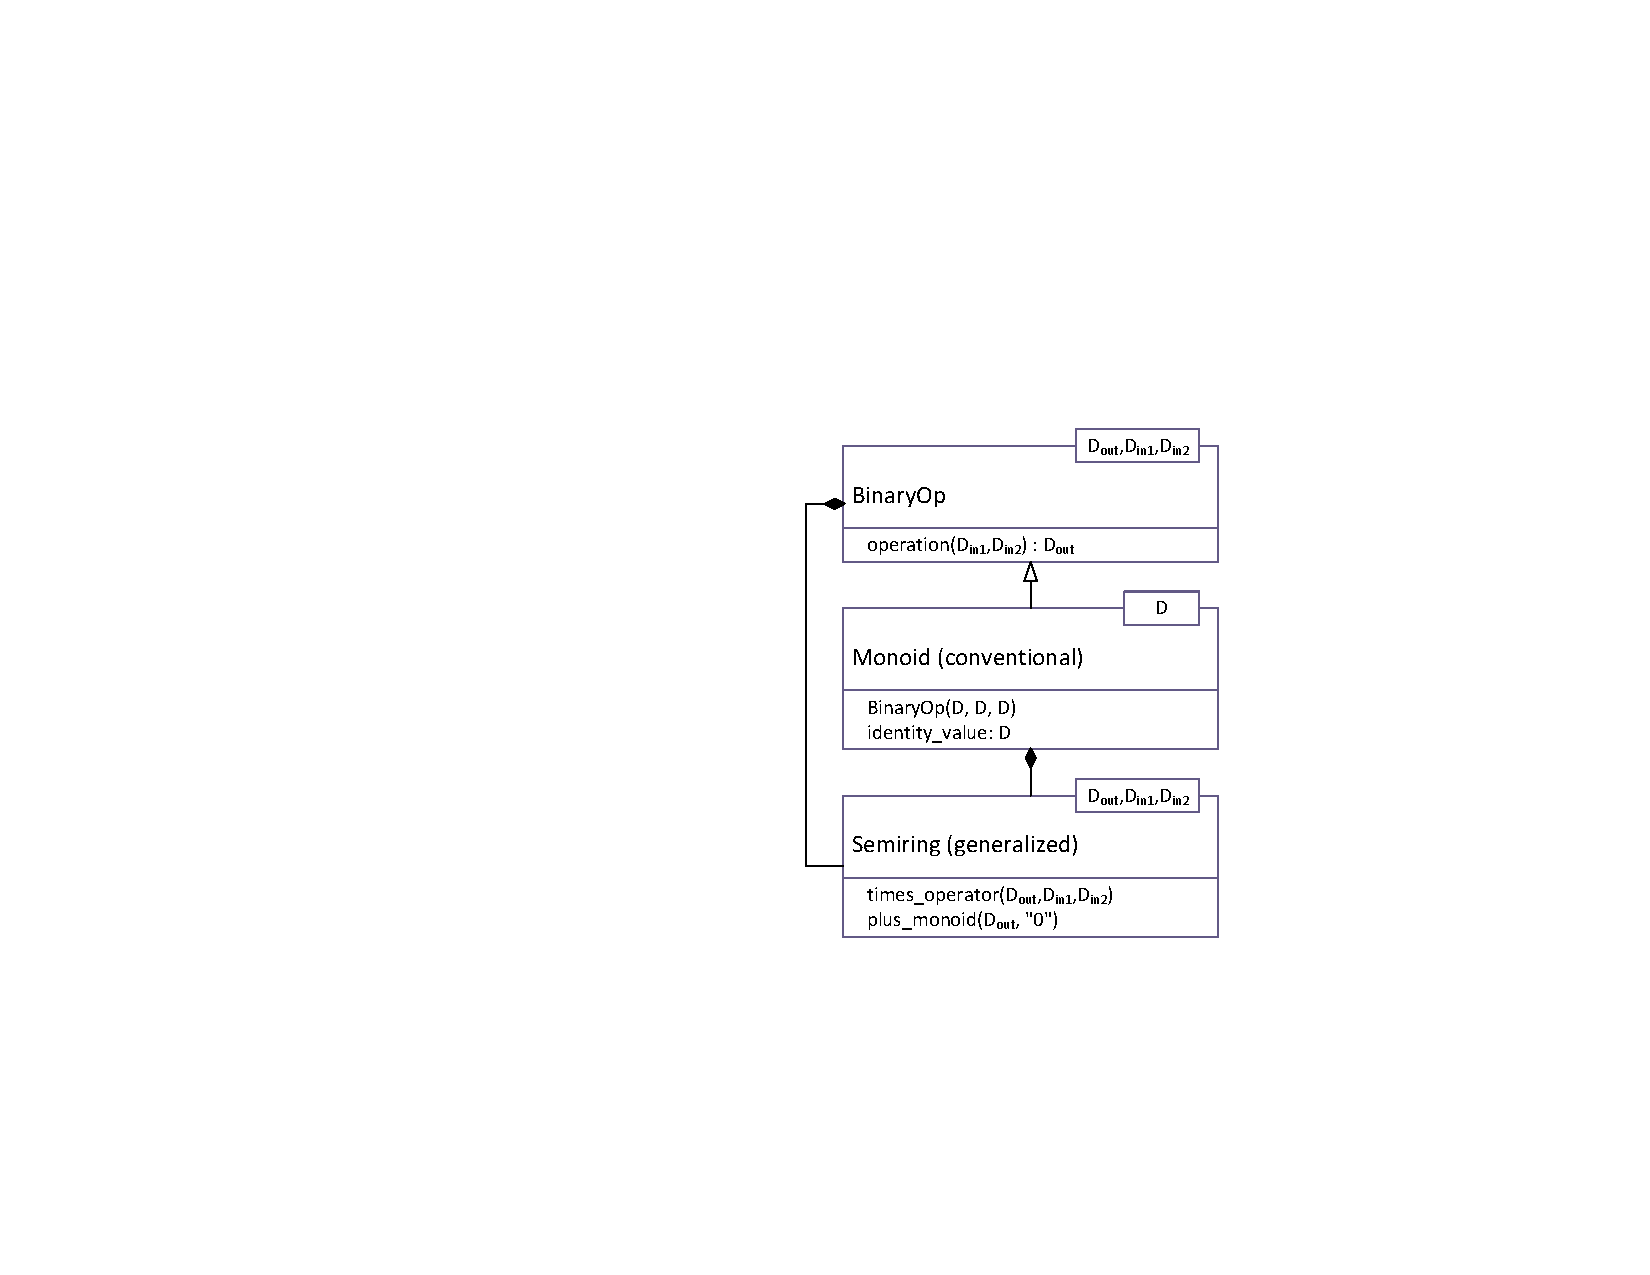
\includegraphics[width=1.0\linewidth,trim=3in 2in 0.5in 2in]{Algebra_Hierarchy_v2_1.pdf}
    \end{center}
    \caption[Hierarchy of algebraic object classes in GraphBLAS.]{Hierarchy of algebraic object classes in GraphBLAS. GraphBLAS 
    semirings consist of a conventional monoid with one domain for the addition 
    function, and a binary operator with three domains for the multiplication function.}
    \label{Fig:AlgebraHierarchy}
    \hrule
\end{figure}

User-defined semirings can be created with calls to {\sf GrB\_Semiring\_new} 
(see Section~\ref{Sec:AlgebraMethods}).
A list of predefined true semirings and convenience
semirings can be found in Tables~\ref{Tab:PredefinedTrueSemirings} and~\ref{Tab:PredefinedUsefulSemirings},
respectively.  Predefined
semirings are named {\sf GrB\_\emph{add}\_\emph{mul}\_SEMIRING\_$T$},
where \emph{add} is the semiring additive operation, \emph{mul} is
the semiring multiplicative operation and $T$ is the domain (type)
of the semiring.

%==================

\begin{table}
\centering
\begin{threeparttable}
\hrule
\caption[Predefined ``true'' semirings for GraphBLAS in C.]{Predefined true semirings 
for GraphBLAS in C where the additive identity is the multiplicative 
annihilator. The $x$ can be one of 8, 16, 32, or 64 in {\sf UINT$x$} or {\sf INT$x$}, 
and can be 32 or 64 in {\sf FP$x$}.}
\label{Tab:PredefinedTrueSemirings}

\hspace*{-1.5em}
\begin{tabular}{l|l|l|l}
                                      & Domains, $T$             & $+$ identity         &                 \\
GraphBLAS identifier              & ($T \times T \rightarrow T$) & $\times$ annihilator & Description     \\ \hline
{\sf GrB\_PLUS\_TIMES\_SEMIRING\_$T$}   & {\sf UINT$x$}            & 0                    & arithmetic semiring \\
                                      & {\sf INT$x$}             & 0                    &                 \\
                                      & {\sf FP$x$}              & 0                    &                 \\
{\sf GrB\_MIN\_PLUS\_SEMIRING\_$T$}     & {\sf UINT$x$}            & {\tt UINT$x$\_MAX}   & min-plus semiring  \\
                                      & {\sf INT$x$}             & {\tt INT$x$\_MAX}    &                 \\
                                      & {\sf FP$x$}              & {\tt INFINITY}       &                 \\
{\sf GrB\_MAX\_PLUS\_SEMIRING\_$T$}     & {\sf INT$x$}             & {\tt INT$x$\_MIN}    & max-plus semiring  \\
                                      & {\sf FP$x$}              & {\tt -INFINITY}      &                 \\
{\sf GrB\_MIN\_TIMES\_SEMIRING\_$T$}    & {\sf UINT$x$}            & {\tt UINT$x$\_MAX}   & min-times semiring \\
{\sf GrB\_MIN\_MAX\_SEMIRING\_$T$}      & {\sf UINT$x$}            & {\tt UINT$x$\_MAX}   & min-max semiring   \\
                                      & {\sf INT$x$}             & {\tt INT$x$\_MAX}    &                 \\
                                      & {\sf FP$x$}              & {\tt INFINITY}       &                 \\
{\sf GrB\_MAX\_MIN\_SEMIRING\_$T$}      & {\sf UINT$x$}            & 0                    & max-min semiring   \\
                                      & {\sf INT$x$}             & {\tt INT$x$\_MIN}    &                 \\
                                      & {\sf FP$x$}              & {\tt -INFINITY}      &                 \\
{\sf GrB\_MAX\_TIMES\_SEMIRING\_$T$}    & {\sf UINT$x$}            & 0                    & max-times semiring \\
{\sf GrB\_PLUS\_MIN\_SEMIRING\_$T$}     & {\sf UINT$x$}            & 0                    & plus-min semiring  \\
                                      &                          &                      &                 \\
{\sf GrB\_LOR\_LAND\_SEMIRING\_BOOL}  & {\sf BOOL}               & {\tt false}          & Logical semiring   \\
{\sf GrB\_LAND\_LOR\_SEMIRING\_BOOL}  & {\sf BOOL}               & {\tt true}           & "and-or" semiring  \\
{\sf GrB\_LXOR\_LAND\_SEMIRING\_BOOL} & {\sf BOOL}               & {\tt false}          & same as {\sf NE\_LAND} \\
{\sf GrB\_LXNOR\_LOR\_SEMIRING\_BOOL} & {\sf BOOL}               & {\tt true}           & same as {\sf EQ\_LOR} \\
\end{tabular}

\hrule
\comment{
\begin{tablenotes}
    \item[1] For {\sf GrB\_ANY\_*\_SEMIRING\_T}, an implementation is free to return any of the results of the application of the "multiply" operator ({\sf FIRST} or {\sf SECOND}), and is not required to always return the same result in different invocations..
\end{tablenotes}
}
\end{threeparttable}
\end{table}

\begin{table}
\centering
\begin{threeparttable}
\hrule
\caption[Other useful predefined semirings for GraphBLAS in C.]{Other useful predefined semirings for GraphBLAS in C that don't have a multiplicative annihilator. 
The $x$ can be one of 8, 16, 32, or 64 in {\sf UINT$x$} or {\sf INT$x$}, 
and can be 32 or 64 in {\sf FP$x$}.}
\label{Tab:PredefinedUsefulSemirings}

\hspace*{-1.5em}
\begin{tabular}{l|l|l|l}
                                    & Domains, $T$             &            &                 \\
GraphBLAS identifier           & ($T \times T \rightarrow T$)  & $+$ identity      & Description             \\ \hline
{\sf GrB\_MAX\_PLUS\_SEMIRING\_$T$}   & {\sf UINT$x$}            & 0                 & max-plus semiring         \\
{\sf GrB\_MIN\_TIMES\_SEMIRING\_$T$}  & {\sf INT$x$}             & {\tt INT$x$\_MAX} & min-times semiring        \\
                                    & {\sf FP$x$}              & {\tt INFINITY}    &                  \\
{\sf GrB\_MAX\_TIMES\_SEMIRING\_$T$}  & {\sf INT$x$}             & {\tt INT$x$\_MIN} & max-times semiring        \\
                                    & {\sf FP$x$}              & {\tt -INFINITY}   &                 \\
{\sf GrB\_PLUS\_MIN\_SEMIRING\_$T$}   & {\sf INT$x$}             & 0                 & plus-min semiring          \\
                                    & {\sf FP$x$}              & 0                 &                 \\ 
{\sf GrB\_MIN\_FIRST\_SEMIRING\_$T$}  & {\sf UINT$x$}            & {\tt UINT$x$\_MAX}& min-select first  semiring     \\
                                    & {\sf INT$x$}             & {\tt INT$x$\_MAX} &                 \\
                                    & {\sf FP$x$}              & {\tt INFINITY}    &                 \\
{\sf GrB\_MIN\_SECOND\_SEMIRING\_$T$} & {\sf UINT$x$}            & {\tt UINT$x$\_MAX}& min-select second semiring     \\
                                    & {\sf INT$x$}             & {\tt INT$x$\_MAX} &                 \\
                                    & {\sf FP$x$}              & {\tt INFINITY}    &                 \\
{\sf GrB\_MAX\_FIRST\_SEMIRING\_$T$}  & {\sf UINT$x$}            & 0                 & max-select first  semiring     \\
                                    & {\sf INT$x$}             & {\tt INT$x$\_MIN} &                 \\
                                    & {\sf FP$x$}              & {\tt -INFINITY}   &                 \\
{\sf GrB\_MAX\_SECOND\_SEMIRING\_$T$} & {\sf UINT$x$}            & 0                 & max-select second semiring     \\
                                    & {\sf INT$x$}             & {\tt INT$x$\_MIN} &                 \\
                                    & {\sf FP$x$}              & {\tt -INFINITY}   &                 \\
\end{tabular}

\hrule
\comment{
\begin{tablenotes}
    \item[1] For {\sf GrB\_ANY\_*\_SEMIRING\_T}, an implementation is free to return any of the results of the application of the "multiply" operator ({\sf FIRST} or {\sf SECOND}), and is not required to always return the same result in different invocations..
\end{tablenotes}
}
\end{threeparttable}
\end{table}

%============================================================================
\section{Collections}

%----------------------------------------------------------------------------
\subsection{Scalars}
\label{Sec:Scalars}

A \emph{GraphBLAS scalar}, $\scalar{s} = \langle D, \{ \sigma \} \rangle$, is defined by
a domain $D$, and a set of zero or one \emph{scalar value}, $\sigma$, where $\sigma \in D$. 
We define $\mathbf{size}(\scalar{s}) = 1$ (constant), and
$\mathbf{L}(\scalar{s}) = \{ \sigma \}$. The set $\mathbf{L}(\scalar{s})$ is
called the \emph{contents} of the GraphBLAS scalar $\scalar{s}$. We also define 
$\mathbf{D}(\scalar{s}) = D$. Finally, $\mathbf{val}(s)$ is a 
reference to the scalar value, $\sigma$, if the GraphBLAS scalar is not empty, and is 
undefined otherwise.

%----------------------------------------------------------------------------
\subsection{Vectors}
\label{Sec:Vectors}

A vector $\vector{v} = \langle D, N, \{ (i,v_i) \} \rangle$ is defined by
a domain $D$, a size $N>0$, and a set of tuples $(i,v_i)$ where $0 \leq
i < N$ and $v_i \in D$. A particular value of $i$ can appear at
most once in $\vector{v}$. We define $\mathbf{size}(\vector{v}) = N$ and
$\mathbf{L}(\vector{v}) = \{ (i,v_i) \}$. The set $\mathbf{L}(\vector{v})$ is
called the \emph{content} of vector $\vector{v}$. We also define the set
$\vector{ind(\vector{v})} = \{ i : (i,v_i) \in \mathbf{L}(\vector{v}) \}$
(called the \emph{structure} of $\vector{v}$), and $\mathbf{D}(\vector{v})
= D$. For a vector $\vector{v}$, $\vector{v}(i)$ is a reference to $v_i$
if $(i,v_i) \in \mathbf{L}(\vector{v})$ and is undefined otherwise.

%----------------------------------------------------------------------------
\subsection{Matrices}
\label{Sec:Matrices}

A matrix $\matrix{A} = \langle D, M, N, \{ (i,j,A_{ij}) \} \rangle$ is
defined by a domain $D$, its number of rows $M>0$, its number of columns
$N>0$, and a set of tuples $(i,j,A_{ij})$ where $0 \leq i < M$, $0 \leq
j < N$, and $A_{ij} \in D$. A particular pair of values $i,j$ can
appear at most once in $\matrix{A}$. We define $\mathbf{ncols}(\matrix{A})
= N$,  $\mathbf{nrows}(\matrix{A}) = M$, and $\mathbf{L}(\matrix{A}) =
\{ (i,j,A_{ij}) \}$.  The set $\mathbf{L}(\matrix{A})$ is called the
\emph{content} of matrix $\matrix{A}$.  We also define the sets
$\vector{indrow(\matrix{A})} = \{ i : \exists (i,j,A_{ij}) \in
\matrix{A} \}$ and $\vector{indcol(\matrix{A})} = \{ j : \exists
(i,j,A_{ij}) \in \matrix{A} \}$.  (These are the sets of nonempty
rows and columns of $\matrix{A}$, respectively.)  The \emph{structure}
of matrix $\matrix{A}$ is the set $\mathbf{ind}(\matrix{A}) = \{ (i,j) :
(i,j,A_{ij}) \in \mathbf{L}(\matrix{A}) \}$, and $\mathbf{D}(\matrix{A}) = D$.
For a matrix $\matrix{A}$, $\matrix{A}(i,j)$ is a reference to $A_{ij}$
if $(i,j,A_{ij}) \in \mathbf{L}(\matrix{A})$ and is undefined otherwise.

If $\matrix{A}$ is a matrix and $0 \leq j < N$, then $\matrix{A}(:,j)
= \langle D, M, \{(i,A_{ij}) : (i,j,A_{ij}) \in \mathbf{L}(\matrix{A})
\} \rangle$ is a vector called the $j$-th \emph{column}
of $\matrix{A}$. Correspondingly, if $\matrix{A}$ is a matrix and
$0 \leq i < M$, then $\matrix{A}(i,:) = \langle D, N, \{(j,A_{ij}) :
(i,j,A_{ij}) \in \mathbf{L}(\matrix{A}) \} \rangle$ is a vector called
the $i$-th \emph{row} of $\matrix{A}$.

Given a matrix $\matrix{A} = \langle D, M, N, \{ (i,j,A_{ij}) \} \rangle$,
its \emph{transpose} is another matrix $\matrix{A}^T = \langle D, N, M, \{
(j,i,A_{ij}) : (i,j,A_{ij}) \in \mathbf{L}(\matrix{A}) \} \rangle$.


%----------------------------------------------------------------------------
\subsection{Masks}
\label{Sec:Masks}

The GraphBLAS C API defines an opaque object called a \emph{mask}.  The mask
is used to control how computed values are stored in the output from a method. 
The mask is an \emph{internal} opaque object; that is, it is never exposed as a 
variable within an application. 

The mask is formed from input objects to the method that uses 
the mask.  For example, a GraphBLAS method may be called with a matrix as the mask
parameter.   The internal mask object is constructed from the input matrix in one
of two ways.  In the default case, an element of the mask is created for each 
tuple that exists in the matrix for which the value of the tuple cast to Boolean 
evaluates to {\tt true}.  Alternatively, the user can specify {\em structure}-only 
behavior where an element of the mask is created for each tuple that exists in 
the matrix {\em regardless} of the value stored in the input matrix.

The internal mask object can be either a one- or a two-dimensional construct.  
One- and two-dimensional masks, described more formally below, are similar to
vectors and matrices, respectively, except that they have structure
(indices) but no values.  When needed, a value is implied for the elements of a 
mask with an implied value of {\tt true} for elements that exist 
and an implied value of {\tt false} for elements that do not exist (\ie,
the locations of the mask that do not have a stored value imply a value of {\tt false}).
Hence, even though a mask does not contain any values, it can be 
considered to imply values from a Boolean domain.

A one-dimensional mask $\vector{m} = \langle N, \{ i \} \rangle$ is
defined by its number of elements $N>0$, and a set $\mathbf{ind}(\vector{m})$
of indices $\{ i \}$ where $0 \leq i < N$.  A particular value of $i$ can
appear at most once in $\vector{m}$. We define $\mathbf{size}(\vector{m})
= N$. The set $\mathbf{ind}(\vector{m})$ is called the \emph{structure} of mask $\vector{m}$.

A two-dimensional mask $\matrix{M} = \langle M, N, \{ (i,j) \}
\rangle$ is defined by its number of rows $M>0$, its number of
columns $N>0$, and a set $\mathbf{ind}(\matrix{M})$ of tuples $(i,j)$
where $0 \leq i < M$, $0 \leq j < N$.   A particular pair of values
$i,j$ can appear at most once in $\matrix{M}$.  We define
$\mathbf{ncols}(\matrix{M}) = N$, and $\mathbf{nrows}(\matrix{M}) = M$.
We also define the sets $\vector{indrow(\matrix{M})} = \{ i : \exists
(i,j) \in \mathbf{ind}(\matrix{M}) \}$ and $\vector{indcol(\matrix{M})}
= \{ j : \exists (i,j) \in \mathbf{ind}(\matrix{M}) \}$.  These are
the sets of nonempty rows and columns of $\matrix{M}$, respectively.
The set $\mathbf{ind}(\matrix{M})$ is called the \emph{structure} of 
mask $\matrix{M}$.

One common operation on masks is the \emph{complement}.
For a one-dimensional mask $\vector{m}$ this is denoted as
$\neg\vector{m}$. For a two-dimensional mask $\matrix{M}$, this is denoted as
$\neg\matrix{M}$.  The complement of a one-dimensional
mask $\vector{m}$ is defined as $\mathbf{ind}(\neg\vector{m}) = \{i : 0
\leq i < N, i \notin \mathbf{ind}(\vector{m}) \}$.  It is the set of all
possible indices that do not appear in $\vector{m}$.  The 
complement of a two-dimensional mask $\matrix{M}$ is defined as the set
$\mathbf{ind}(\neg\matrix{M}) = \{(i,j)$ : $0 \leq i < M$, $0 \leq j < N$,
$(i,j) \notin \mathbf{ind}(\matrix{M}) \}$.  It is the set of all possible
indices that do not appear in $\matrix{M}$.



%-----------------------------------------------------------------------------

%\chapter{Methods \scott{Rename to Operations}}
%\label{Chp:Methods}

%This chapter defines the behavior of all the methods in the GraphBLAS C API.
%All methods can be declared for use in programs by including the {\tt GraphBLAS.h} header file.

%\section{Context methods}

The methods in this section set up and tear down the GraphBLAS
context within which all GraphBLAS methods must be executed.  The initialization
of this context also includes the specification of which execution mode is
to be used.

%-----------------------------------------------------------------------------
\subsection{{\sf init}: Initialize a GraphBLAS context}

Creates and initializes a GraphBLAS C API context.

\paragraph{\syntax}

\begin{verbatim}
        GrB_Info GrB_init(GrB_Mode mode);
\end{verbatim}


\paragraph{Parameters}

\begin{itemize}[leftmargin=1.1in]
	\item[{\sf mode}] Mode for the GraphBLAS context. Must be either {\sf GrB\_BLOCKING}
    or {\sf GrB\_NONBLOCKING}.
\end{itemize}

\paragraph{Return Values}

\begin{itemize}[leftmargin=2.1in]
\item[{\sf GrB\_SUCCESS}]           operation completed successfully.
\item[{\sf GrB\_PANIC}]             unknown internal error.
\item[{\sf GrB\_INVALID\_VALUE}]    invalid mode specified, or method called multiple times.
\end{itemize}

\paragraph{Description}

The {\sf init} method creates and initializes a GraphBLAS C API context.  The argument
to {\sf GrB\_init} defines the mode for the context.  The two
available modes are:

\begin{itemize}
\item {\sf GrB\_BLOCKING}: In this mode, each method in a sequence returns after
its computations have completed and output arguments are available to
subsequent statements in an application.  When executing in {\sf
GrB\_BLOCKING} mode, the methods execute in program order.

\item {\sf GrB\_NONBLOCKING}: In this mode, methods in a sequence may return after arguments
in the method have been tested for dimension and domain compatibility
within the method but potentially before their computations complete.  Output
arguments are available to subsequent GraphBLAS methods in an application.
When executing in {\sf GrB\_NONBLOCKING} mode, the methods in a sequence
may execute in any order that preserves the mathematical result defined
by the sequence.
\end{itemize}

An application can only create one context per execution instance.  An application
may only call {\sf GrB\_Init} once.  Calling {\sf GrB\_Init} more
than once results in undefined behavior.

%-----------------------------------------------------------------------------
\subsection{{\sf finalize}: Finalize a GraphBLAS context}
\label{Sec:GrB_finalize}

Terminates and frees any internal resources created to support the
GraphBLAS C API context.

\paragraph{\syntax}

\begin{verbatim}
        GrB_Info GrB_finalize();
\end{verbatim}

\paragraph{Return Values}

\begin{itemize}[leftmargin=2.1in]
\item[{\sf GrB\_SUCCESS}]        operation completed successfully.
\item[{\sf GrB\_PANIC}]          unknown internal error.
\end{itemize}

\paragraph{Description}

The {\sf finalize} method terminates and frees any internal resources created to support the
GraphBLAS C API context.  {\sf GrB\_finalize} may only be called after
a context has been initialized by calling {\sf GrB\_init}, or else undefined
behavior occurs.  After {\sf GrB\_finalize}
has been called to finalize a GraphBLAS context, calls to any GraphBLAS methods,
including {\sf GrB\_finalize}, will result in undefined behavior.


%-----------------------------------------------------------------------------
\subsection{{\sf getVersion}: Get the version number of the standard.}

Query the library for the version number of the standard that this library
implements.

\paragraph{\syntax}

\begin{verbatim}
        GrB_Info GrB_getVersion(unsigned int *version,
                                unsigned int *subversion);
\end{verbatim}


\paragraph{Parameters}

\begin{itemize}[leftmargin=1.1in]
	\item[{\sf version}] ({\sf OUT})  On successful return will hold the value
    of the major version number.
	\item[{\sf subversion}] ({\sf OUT})  On successful return will hold the value
    of the subversion number.
\end{itemize}


\paragraph{Return Values}

\begin{itemize}[leftmargin=2.1in]
\item[{\sf GrB\_SUCCESS}]        operation completed successfully.
\item[{\sf GrB\_PANIC}]          unknown internal error.
\end{itemize}

\paragraph{Description}

The {\sf getVersion} method is used to query the major and minor version number of the
GraphBLAS C API specification that the library implements at runtime.  To
support compile time queries the following two macros shall also be defined by
the library.
\begin{verbatim}
        #define GRB_VERSION     2
        #define GRB_SUBVERSION  0
\end{verbatim}


%\section{Object methods}

This section describes methods that setup and operate on GraphBLAS opaque objects
but are not part of the the GraphBLAS math specification.

%\subsection{Algebra methods}
\label{Sec:AlgebraMethods}

%-----------------------------------------------------------------------------

\subsubsection{{\sf Type\_new}: Construct a new GraphBLAS (user-defined) type}
\label{Sec:TypeNew}

Creates a new user-defined GraphBLAS type. This type can then be used to create new
operators, monoids, semirings, vectors and matrices.

\paragraph{\syntax}

\begin{verbatim}
        GrB_Info GrB_Type_new(GrB_Type  *utype,
                              size_t     sizeof(ctype));
\end{verbatim}

\paragraph{Parameters}

\begin{itemize}[leftmargin=1.1in]
    \item[{\sf utype}] ({\sf INOUT}) On successful return, contains a handle 
                                     to the newly created user-defined GraphBLAS 
                                     type object.
	\item[{\sf ctype}] ({\sf IN})    A C type that defines the new GraphBLAS 
                                     user-defined type.
\end{itemize}

\paragraph{Return Values}

\begin{itemize}[leftmargin=2.1in]
\item[{\sf GrB\_SUCCESS}]           operation completed successfully.
\item[{\sf GrB\_PANIC}]             unknown internal error.
\item[{\sf GrB\_OUT\_OF\_MEMORY}]          not enough memory available for operation.
\item[{\sf GrB\_NULL\_POINTER}]    {\sf utype} pointer is {\sf NULL}.
\end{itemize}

\paragraph{Description}

Given a C type {\sf ctype}, the {\sf Type\_new} method returns in {\sf utype} a handle to
a new GraphBLAS type that is equivalent to the C type.  Variables of this {\sf ctype} 
must be a struct, union, or fixed-size array. In particular, given two variables, 
{\tt src} and {\tt dst}, of type {\sf ctype}, the following operation must be a 
valid way to copy the contents of {\tt src} to {\tt dst}:

\begin{center}
{\tt memcpy(\&dst, \&src, sizeof({\sf ctype}))}
\end{center}

A new, user-defined type {\sf utype} should be destroyed with a call to 
{\sf GrB\_free(utype)} when no longer needed.

It is not an error to call this method more than once on the same variable;  
however, the handle to the previously created object will be overwritten. 

%-----------------------------------------------------------------------------
\subsubsection{{\sf UnaryOp\_new}: Construct a new GraphBLAS unary operator}

Initializes a new GraphBLAS unary operator with a specified user-defined 
function and its types (domains).

\paragraph{\syntax}

\begin{verbatim}
        GrB_Info GrB_UnaryOp_new(GrB_UnaryOp *unary_op,
                                 void       (*unary_func)(void*, const void*),
                                 GrB_Type     d_out,
                                 GrB_Type     d_in);
\end{verbatim}

\paragraph{Parameters}

\begin{itemize}[leftmargin=1.1in]
    \item[{\sf unary\_op}] ({\sf INOUT}) On successful return, contains a
                           handle to the newly created GraphBLAS unary operator object.
    \item[{\sf unary\_func}] ({\sf IN})  a pointer to a user-defined function that takes 
                           one input parameter of {\sf d\_in}'s type
			   and returns a value of {\sf d\_out}'s type, both passed as {\sf void} pointers.
                           Specifically the signature of the function is expected to 
                           be of the form:
          \begin{verbatim}
          void func(void *out, const void *in);
          \end{verbatim}
    \item[{\sf d\_out}] ({\sf IN})  The {\sf GrB\_Type} of the return value of the unary 
                           operator being created.  Should be one of the predefined 
                           GraphBLAS types in Table~\ref{Tab:PredefinedTypes}, or a 
                           user-defined GraphBLAS type.
    \item[{\sf d\_in}] ({\sf IN})  The {\sf GrB\_Type} of the input 
                           argument of the unary operator being created.  Should be 
                           one of the predefined GraphBLAS types in 
                           Table~\ref{Tab:PredefinedTypes}, or a user-defined GraphBLAS type.
\end{itemize}

\paragraph{Return Values}

\begin{itemize}[leftmargin=2.1in]
\item[{\sf GrB\_SUCCESS}]           operation completed successfully.
\item[{\sf GrB\_PANIC}]             unknown internal error.
\item[{\sf GrB\_OUT\_OF\_MEMORY}]          not enough memory available for operation.
\item[{\sf GrB\_UNINITIALIZED\_OBJECT}]          any {\sf GrB\_Type} parameter (for
                                    user-defined types) has not been
                                    initialized by a call to {\sf GrB\_Type\_new}.
\item[{\sf GrB\_NULL\_POINTER}]    {\sf unary\_op} or {\sf unary\_func}
                                    pointers are {\sf NULL}.

%\item[{\sf GrB\_DOMAIN\_MISMATCH}]  the types in the function pointer signature
%                                    are not compatible with the {\sf GrB\_Type}
%                                    parameters specified when user-defined types
%                                    are specified.
\end{itemize}

\paragraph{Description}

\newenvironment{code}{\tt}{}

The {\sf UnaryOp\_new} method creates a new GraphBLAS unary operator
\begin{quote}
$f_u = \langle \mathbf{D}({\sf d\_out}), \mathbf{D}({\sf d\_in}), {\sf unary\_func} \rangle$
\end{quote}
and returns a handle to it in {\sf unary\_op}.

The implementation of {\sf unary\_func} must be such that it works
even if the {\sf d\_out} and {\sf d\_in} arguments are aliased.
In other words, for all invocations of the function:
\begin{quote}
\begin{verbatim}
unary_func(out,in);
\end{verbatim}
\end{quote}
the value of {\sf out} must be the same as if the following code
was executed:

\begin{quote}
\begin{code}
    $\mathbf{D}({\sf d\_in})$ *tmp = malloc(sizeof($\mathbf{D}({\sf d\_in}$))); \\
    memcpy(tmp,in,sizeof($\mathbf{D}({\sf d\_in}$))); \\
    unary\_func(out,tmp); \\
    free(tmp);
\end{code}
\end{quote}

It is not an error to call this method more than once on the same variable;  
however, the handle to the previously created object will be overwritten. 

%-----------------------------------------------------------------------------

\subsubsection{{\sf BinaryOp\_new}: Construct a new GraphBLAS binary operator}

Initializes a new GraphBLAS binary operator with a specified user-defined 
function and its types (domains).

\paragraph{\syntax}

\begin{verbatim}
        GrB_Info GrB_BinaryOp_new(GrB_BinaryOp *binary_op,
                                  void        (*binary_func)(void*,
                                                             const void*,
                                                             const void*),
                                  GrB_Type      d_out,
                                  GrB_Type      d_in1,
                                  GrB_Type      d_in2);
\end{verbatim}

\paragraph{Parameters}

\begin{itemize}[leftmargin=1.1in]
    \item[{\sf binary\_op}] ({\sf INOUT}) On successful return, contains a 
          handle to the newly created GraphBLAS binary operator object.
    \item[{\sf binary\_func}] ({\sf IN}) A pointer to a user-defined function that 
          takes two input parameters of types {\sf d\_in1} and {\sf d\_in2} and returns a value of
		type {\sf d\_out}, all passed as {\sf void} pointers.
          Specifically the signature of the function is expected to 
          be of the form:
      \begin{verbatim}
      void func(void *out, const void *in1, const void *in2);
      \end{verbatim}
    \item[{\sf d\_out}]  ({\sf IN}) The {\sf GrB\_Type} of the return
          value of the binary operator being created. Should be one of the
          predefined GraphBLAS types in Table~\ref{Tab:PredefinedTypes}, or a 
          user-defined GraphBLAS type.
    \item[{\sf d\_in1}]  ({\sf IN}) The {\sf GrB\_Type} of the left hand 
          argument of the binary operator being created. Should be one of the
          predefined GraphBLAS types in Table~\ref{Tab:PredefinedTypes}, or a
          user-defined GraphBLAS type.
    \item[{\sf d\_in2}]  ({\sf IN}) The {\sf GrB\_Type} of the right hand 
          argument of the binary operator being created. Should be one of the
          predefined GraphBLAS types in Table~\ref{Tab:PredefinedTypes}, or a 
          user-defined GraphBLAS type.
\end{itemize}

\paragraph{Return Values}

\begin{itemize}[leftmargin=2.1in]
\item[{\sf GrB\_SUCCESS}]           operation completed successfully.
\item[{\sf GrB\_PANIC}]             unknown internal error.
\item[{\sf GrB\_OUT\_OF\_MEMORY}]          not enough memory available for operation.
\item[{\sf GrB\_UNINITIALIZED\_OBJECT}]          the {\sf GrB\_Type} (for user-defined types)
                                    has not been initialized by a call to {\sf GrB\_Type\_new}.
\item[{\sf GrB\_NULL\_POINTER}]    {\sf binary\_op} or {\sf binary\_func} pointer is {\sf NULL}.

%\item[{\sf GrB\_DOMAIN\_MISMATCH}]  the types in the function pointer signature are not   
%                                    compatible with the {\sf GrB\_Type} parameters specified.
\end{itemize}

\paragraph{Description}

The {\sf BinaryOp\_new} methods creates a new GraphBLAS binary operator
\begin{quote}
$f_b = \langle \mathbf{D}({\sf d\_out}), \mathbf{D}({\sf d\_in1}), \mathbf{D}({\sf d\_in2}), {\sf binary\_func} \rangle$
\end{quote}
and returns a handle to it in {\sf binary\_op}.

The implementation of {\sf binary\_func} must be such that it works
even if any of the {\sf d\_out}, {\sf d\_in1}, and {\sf d\_in2} arguments are aliased to each other.
In other words, for all invocations of the function:
\begin{quote}
\begin{verbatim}
binary_func(out,in1,in2);
\end{verbatim}
\end{quote}
the value of {\sf out} must be the same as if the following code
was executed:

\begin{quote}
\begin{code}
    $\mathbf{D}({\sf d\_in1})$ *tmp1 = malloc(sizeof($\mathbf{D}({\sf d\_in1}$))); \\
    $\mathbf{D}({\sf d\_in2})$ *tmp2 = malloc(sizeof($\mathbf{D}({\sf d\_in2}$))); \\
    memcpy(tmp1,in1,sizeof($\mathbf{D}({\sf d\_in1}$))); \\
    memcpy(tmp2,in2,sizeof($\mathbf{D}({\sf d\_in2}$))); \\
    binary\_func(out,tmp1,tmp2); \\
    free(tmp2); \\
    free(tmp1);
\end{code}
\end{quote}

It is not an error to call this method more than once on the same variable;  
however, the handle to the previously created object will be overwritten. 

%-----------------------------------------------------------------------------

\subsubsection{{\sf Monoid\_new}: Construct a new GraphBLAS monoid}

Creates a new monoid with specified binary operator and identity value.

\paragraph{\syntax}

\begin{verbatim}
        GrB_Info GrB_Monoid_new(GrB_Monoid    *monoid,
                                GrB_BinaryOp   binary_op,
                                <type>         identity);
\end{verbatim}

\paragraph{Parameters}

\begin{itemize}[leftmargin=1.1in]
    \item[{\sf monoid}] ({\sf INOUT}) On successful return, contains a
                         handle to the newly created GraphBLAS monoid object.
    \item[{\sf binary\_op}] ({\sf IN}) An existing GraphBLAS associative binary 
                         operator whose input and output types are the same.
    \item[{\sf identity}]  ({\sf IN}) The value of the identity element of the 
                         monoid. Must be the same type as the type used by the
                         {\sf binary\_op} operator.
\end{itemize}

\paragraph{Return Values}

\begin{itemize}[leftmargin=2.1in]
\item[{\sf GrB\_SUCCESS}]           operation completed successfully.
\item[{\sf GrB\_PANIC}]             unknown internal error.
\item[{\sf GrB\_OUT\_OF\_MEMORY}]   not enough memory available for operation.
\item[{\sf GrB\_UNINITIALIZED\_OBJECT}]  the {\sf GrB\_BinaryOp} (for user-defined operators) has not been
                                    initialized by a call to {\sf GrB\_BinaryOp\_new}.
\item[{\sf GrB\_NULL\_POINTER}]     {\sf monoid} pointer is {\sf NULL}.
\item[{\sf GrB\_DOMAIN\_MISMATCH}]  all three argument types of the binary operator and
                                    the type of the identity value are not the same.
\end{itemize}

\paragraph{Description}

The {\sf Monoid\_new} method creates a new monoid $M = \langle \mathbf{D}({\sf binary\_op}), {\sf binary\_op}, 
{\sf identity} \rangle$ and returns a handle to it in {\sf monoid}.

If {\sf binary\_op} is not associative, the results of GraphBLAS operations that
require associativity of this monoid will be undefined.

It is not an error to call this method more than once on the same variable;  
however, the handle to the previously created object will be overwritten. 

%-----------------------------------------------------------------------------
\subsubsection{{\sf Semiring\_new}: Construct a new GraphBLAS semiring}

Creates a new semiring with specified domain, operators, and elements.

\paragraph{\syntax}

\begin{verbatim}
        GrB_Info GrB_Semiring_new(GrB_Semiring  *semiring,
                                  GrB_Monoid     add_op,
                                  GrB_BinaryOp   mul_op);
\end{verbatim}

\paragraph{Parameters}

\begin{itemize}[leftmargin=1.1in]
    \item[{\sf semiring}] ({\sf INOUT}) On successful return, contains a 
    handle to the newly created GraphBLAS semiring.
    \item[{\sf add\_op}]  ({\sf IN}) An existing GraphBLAS commutative monoid that 
    specifies the addition operator and its identity.
    \item[{\sf mul\_op}]  ({\sf IN}) An existing GraphBLAS binary operator that 
    specifies the semiring's multiplication operator. In addition, {\sf mul\_op}'s
    output domain, $\bDout({\sf mul\_op})$, must be the same as the {\sf add\_op}'s
    domain $\mathbf{D}(\mbox{\sf add\_op})$.
\end{itemize}


\paragraph{Return Values}

\begin{itemize}[leftmargin=2.1in]
\item[{\sf GrB\_SUCCESS}]           operation completed successfully.
\item[{\sf GrB\_PANIC}]             unknown internal error.
\item[{\sf GrB\_OUT\_OF\_MEMORY}]   not enough memory available for this method to complete.
\item[{\sf GrB\_UNINITIALIZED\_OBJECT}]   the {\sf add\_op} (for user-define monoids) object has not been
                                    initialized with a call to {\sf GrB\_Monoid\_new}
				    or the {\sf mul\_op} (for user-defined operators) object has not been
                                    not been initialized by a call to 
                                    {\sf GrB\_BinaryOp\_new}.
\item[{\sf GrB\_NULL\_POINTER}]    {\sf semiring} pointer is {\sf NULL}.
\item[{\sf GrB\_DOMAIN\_MISMATCH}]  the output domain of {\sf mul\_op} does not
                                    match the domain of the {\sf add\_op} monoid.
\end{itemize}

\paragraph{Description}

The {\sf Semiring\_new} method creates a new semiring:
\begin{quote}
$S = \langle \bDout({\sf mul\_op}), 
\bDin1({\sf mul\_op}), \bDin2({\sf mul\_op}), {\sf add\_op}, 
{\sf mul\_op}, \mathbf{0}({\sf add\_op})\rangle$
\end{quote}
and returns a handle to it in 
{\sf semiring}.  Note that $\bDout({\sf mul\_op})$ must be the same as 
$\mathbf{D}({\sf add\_op})$.

If {\sf add\_op} is not commutative, then GraphBLAS operations using this semiring
will be undefined.

It is not an error to call this method more than once on the same variable;  
however, the handle to the previously created object will be overwritten. 

%-----------------------------------------------------------------------------

\subsubsection{{\sf IndexUnaryOp\_new}: Construct a new GraphBLAS index unary operator}

Initializes a new GraphBLAS index unary operator with a specified user-defined 
function and its types (domains).

\paragraph{\syntax}

\begin{verbatim}
    GrB_Info GrB_IndexUnaryOp_new(GrB_IndexUnaryOp   *index_unary_op,
                                  void (*index_unary_func)(void*,
                                                           const void*,
                                                           GrB_Index,
                                                           GrB_Index,
                                                           const void*),
                                  GrB_Type            d_out,
                                  GrB_Type            d_in1,
                                  GrB_Type            d_in2);
\end{verbatim}

\paragraph{Parameters}

\begin{itemize}[leftmargin=1.2in]
    \item[{\sf index\_unary\_op}] ({\sf INOUT}) On successful return, contains a 
          handle to the newly created GraphBLAS index unary operator object.
    \item[{\sf index\_unary\_func}] ({\sf IN}) A pointer to a user-defined 
          function that takes input parameters of types {\sf d\_in1}, 
          {\sf GrB\_Index}, {\sf GrB\_Index} and {\sf d\_in2}
          and returns a value of type {\sf d\_out}.  Except for the {\sf GrB\_Index}
          parameters, all are passed as {\sf void} pointers.
          Specifically the signature of the function is expected to 
          be of the form:
      \begin{verbatim}
      void func(void       *out,
                const void *in1,
                GrB_Index   row_index,
                GrB_Index   col_index, 
                const void *in2);
      \end{verbatim}
    \item[{\sf d\_out}]  ({\sf IN}) The {\sf GrB\_Type} of the return
          value of the index unary operator being created. Should be one of the
          predefined GraphBLAS types in Table~\ref{Tab:PredefinedTypes}, or a 
          user-defined GraphBLAS type.
    \item[{\sf d\_in1}]  ({\sf IN}) The {\sf GrB\_Type} of the first input 
          argument of the index unary operator being created and corresponds to
          the stored values of the {\sf GrB\_Vector} or {\sf GrB\_Matrix} being
          operated on. Should be one of the predefined GraphBLAS types in
          Table~\ref{Tab:PredefinedTypes}, or a user-defined GraphBLAS type.
    \item[{\sf d\_in2}]  ({\sf IN}) The {\sf GrB\_Type} of the last input
          argument of the index unary operator being created and corresponds to
          a scalar provided by the GraphBLAS operation that uses this operator.
          Should be one of the predefined GraphBLAS types in 
          Table~\ref{Tab:PredefinedTypes}, or a user-defined GraphBLAS type.
\end{itemize}

\paragraph{Return Values}

\begin{itemize}[leftmargin=2.1in]
\item[{\sf GrB\_SUCCESS}]           operation completed successfully.
\item[{\sf GrB\_PANIC}]             unknown internal error.
\item[{\sf GrB\_OUT\_OF\_MEMORY}]          not enough memory available for operation.
\item[{\sf GrB\_UNINITIALIZED\_OBJECT}]          the {\sf GrB\_Type} (for user-defined types)
                                    has not been initialized by a call to {\sf GrB\_Type\_new}.
\item[{\sf GrB\_NULL\_POINTER}]    {\sf index\_unary\_op} or {\sf index\_unary\_func} pointer is {\sf NULL}.

%\jose{Domain mistmatch not possible.}
%\item[{\sf GrB\_DOMAIN\_MISMATCH}]  the types in the function pointer signature are not   
%                                    compatible with the {\sf GrB\_Type} parameters specified.
\end{itemize}

\paragraph{Description}

The {\sf IndexUnaryOp\_new} methods creates a new GraphBLAS index unary operator
\begin{quote}
$f_{i} = \langle \mathbf{D}({\sf d\_out}), \mathbf{D}({\sf d\_in1}), \mathbf{D}({\sf GrB\_Index}), \mathbf{D}({\sf GrB\_Index}), \mathbf{D}({\sf d\_in2}), {\sf index\_unary\_func} \rangle$
\end{quote}
and returns a handle to it in {\sf index\_unary\_op}.

The implementation of {\sf index\_unary\_func} must be such that it works
even if any of the {\sf d\_out}, {\sf d\_in1}, and {\sf d\_in2} arguments are aliased to each other.
In other words, for all invocations of the function:
\begin{quote}
\begin{verbatim}
index_unary_func(out,in1,row_index,col_index,n,in2);
\end{verbatim}
\end{quote}
the value of {\sf out} must be the same as if the following code
was executed (shown here for matrices):

\begin{quote}
\begin{code}
    GrB\_Index row\_index = ...;\\
    GrB\_Index col\_index = ...;\\
    $\mathbf{D}({\sf d\_in1})$ *tmp1 = malloc(sizeof($\mathbf{D}({\sf d\_in1}$))); \\
    $\mathbf{D}({\sf d\_in2})$ *tmp2 = malloc(sizeof($\mathbf{D}({\sf d\_in2}$))); \\
    memcpy(tmp1,in1,sizeof($\mathbf{D}({\sf d\_in1}$))); \\
    memcpy(tmp2,in2,sizeof($\mathbf{D}({\sf d\_in2}$))); \\
    index\_unary\_func(out,tmp1,row\_index,col\_index,tmp2); \\
    free(tmp2); \\
    free(tmp1);
\end{code}
\end{quote}

It is not an error to call this method more than once on the same variable;  
however, the handle to the previously created object will be overwritten. 

%%-----------------------------------------------------------------------------
\subsection{Scalar methods}


%-----------------------------------------------------------------------------
\subsubsection{{\sf Scalar\_new}: Construct a new scalar}

Creates a new empty scalar with specified domain.

\paragraph{\syntax}

\begin{verbatim}
        GrB_Info GrB_Scalar_new(GrB_Scalar *s,
                                GrB_Type    d);
\end{verbatim}

\paragraph{Parameters}

\begin{itemize}[leftmargin=1.1in]
    \item[{\sf s}] ({\sf INOUT}) On successful return, contains a handle
                                 to the newly created GraphBLAS scalar.
    \item[{\sf d}] ({\sf IN})    The type corresponding to the domain of the 
                                 scalar being created.  Can be one of the 
                                 predefined GraphBLAS types in 
                                 Table~\ref{Tab:PredefinedTypes}, or an existing 
                                 user-defined GraphBLAS type.
\end{itemize}

\paragraph{Return Values}

\begin{itemize}[leftmargin=2.1in]
    \item[{\sf GrB\_SUCCESS}]         In blocking mode, the operation completed
    successfully. In non-blocking mode, this indicates that the API checks 
    for the input arguments passed successfully. Either way, output scalar 
    {\sf s} is ready to be used in the next method of the sequence.

    \item[{\sf GrB\_PANIC}]           Unknown internal error.
    
    \item[{\sf GrB\_INVALID\_OBJECT}] This is returned in any execution mode 
    whenever one of the opaque GraphBLAS objects (input or output) is in an invalid 
    state caused by a previous execution error.  Call {\sf GrB\_error()} to access 
    any error messages generated by the implementation.

    \item[{\sf GrB\_OUT\_OF\_MEMORY}] Not enough memory available for operation.
    
    \item[{\sf GrB\_UNINITIALIZED\_OBJECT}]  The {\sf GrB\_Type} object has not 
    been initialized by a call to {\sf GrB\_Type\_new} (needed for user-defined types).
    
    \item[{\sf GrB\_NULL\_POINTER}]  The {\sf s} pointer is {\sf NULL}.
\end{itemize}

\paragraph{Description}

Creates a new GraphBLAS scalar $\scalar{s}$ of domain $\mathbf{D}({\sf d})$ and empty 
$\mathbf{L}(\scalar{s})$. The method returns a handle to the new scalar in {\sf s}.

It is not an error to call this method more than once on the same variable;  
however, the handle to the previously created object will be overwritten. 

%-----------------------------------------------------------------------------
\subsubsection{{\sf Scalar\_dup}: Construct a copy of a GraphBLAS scalar}

Creates a new scalar with the same domain and contents as another scalar.

\paragraph{\syntax}

\begin{verbatim}
        GrB_Info GrB_Scalar_dup(GrB_Scalar       *t,
                                const GrB_Scalar  s);
\end{verbatim}

\paragraph{Parameters}

\begin{itemize}[leftmargin=1.1in]
    \item[{\sf t}]  ({\sf INOUT}) On successful return, contains a handle
                                  to the newly created GraphBLAS scalar.
    \item[{\sf s}]  ({\sf IN})    The GraphBLAS scalar to be duplicated.
\end{itemize}

\paragraph{Return Values}

\begin{itemize}[leftmargin=2.1in]
    \item[{\sf GrB\_SUCCESS}]         In blocking mode, the operation completed
    successfully. In non-blocking mode, this indicates that the API checks 
    for the input arguments passed successfully. Either way, output scalar 
    {\sf t} is ready to be used in the next method of the sequence.

    \item[{\sf GrB\_PANIC}]           Unknown internal error.
    
    \item[{\sf GrB\_INVALID\_OBJECT}] This is returned in any execution mode 
    whenever one of the opaque GraphBLAS objects (input or output) is in an invalid 
    state caused by a previous execution error.  Call {\sf GrB\_error()} to access 
    any error messages generated by the implementation.

    \item[{\sf GrB\_OUT\_OF\_MEMORY}] Not enough memory available for operation.
    
    \item[{\sf GrB\_UNINITIALIZED\_OBJECT}]  The GraphBLAS scalar, {\sf s}, has 
    not been initialized by a call to {\sf Scalar\_new} or {\sf Scalar\_dup}.
    
    \item[{\sf GrB\_NULL\_POINTER}]  The {\sf t} pointer is {\sf NULL}.
\end{itemize}

\paragraph{Description}

Creates a new scalar $\scalar{t}$ of domain $\mathbf{D}({\sf s})$ and contents 
$\mathbf{L}({\sf s})$. The method returns a handle to the new scalar in {\sf t}.

It is not an error to call this method more than once with the same output variable;  
however, the handle to the previously created object will be overwritten. 


%-----------------------------------------------------------------------------
\subsubsection{{\sf Scalar\_clear}: Clear/remove a stored value from a scalar}

Removes the stored value from a scalar.

\paragraph{\syntax}

\begin{verbatim}
        GrB_Info GrB_Scalar_clear(GrB_Scalar s);
\end{verbatim}

\paragraph{Parameters}

\begin{itemize}[leftmargin=1.1in]
    \item[{\sf s}] ({\sf INOUT}) An existing GraphBLAS scalar to clear.
\end{itemize}

\paragraph{Return Values}

\begin{itemize}[leftmargin=2.1in]
    \item[{\sf GrB\_SUCCESS}]         In blocking mode, the operation completed
    successfully. In non-blocking mode, this indicates that the API checks 
    for the input arguments passed successfully. Either way, output scalar 
    {\sf s} is ready to be used in the next method of the sequence.

    \item[{\sf GrB\_PANIC}]           Unknown internal error.
    
    \item[{\sf GrB\_INVALID\_OBJECT}] This is returned in any execution mode 
    whenever one of the opaque GraphBLAS objects (input or output) is in an invalid 
    state caused by a previous execution error.  Call {\sf GrB\_error()} to access 
    any error messages generated by the implementation.

    \item[{\sf GrB\_OUT\_OF\_MEMORY}] Not enough memory available for operation.
    
    \item[{\sf GrB\_UNINITIALIZED\_OBJECT}]  The GraphBLAS scalar, {\sf s}, has 
    not been initialized by a call to {\sf Scalar\_new} or {\sf Scalar\_dup}.
    
\end{itemize}

\paragraph{Description}

Removes the stored value from an existing scalar. After the call, 
$\mathbf{L}({\sf s})$ is empty. The size of the scalar does not change. 


%-----------------------------------------------------------------------------
\subsubsection{{\sf Scalar\_nvals}: Number of stored elements in a scalar}
\label{Sec:Scalar_nvals}

Retrieve the number of stored elements in a scalar (either zero or one).

\paragraph{\syntax}

\begin{verbatim}
        GrB_Info GrB_Scalar_nvals(GrB_Index        *nvals,
                                  const GrB_Scalar  s);
\end{verbatim}

\paragraph{Parameters}

\begin{itemize}[leftmargin=1.1in]
    \item[{\sf nvals}] ({\sf OUT}) On successful return, this is set to the number of 
                                   stored elements in the scalar (zero or one).
    \item[{\sf s}]     ({\sf IN})  An existing GraphBLAS scalar being queried.
\end{itemize}


\paragraph{Return Values}

\begin{itemize}[leftmargin=2.1in]
    \item[{\sf GrB\_SUCCESS}]  In blocking or non-blocking mode, the operation 
    completed successfully and the value of {\sf nvals} has been set. 

    \item[{\sf GrB\_PANIC}]    Unknown internal error.
    
    \item[{\sf GrB\_INVALID\_OBJECT}] This is returned in any execution mode 
    whenever one of the opaque GraphBLAS objects (input or output) is in an invalid 
    state caused by a previous execution error.  Call {\sf GrB\_error()} to access 
    any error messages generated by the implementation.

    \item[{\sf GrB\_OUT\_OF\_MEMORY}] Not enough memory available for operation.
    
    \item[{\sf GrB\_UNINITIALIZED\_OBJECT}]  The GraphBLAS scalar, {\sf s}, has 
    not been initialized by a call to {\sf Scalar\_new} or {\sf Scalar\_dup}.
    
    \item[{\sf GrB\_NULL\_POINTER}]  The {\sf nvals} pointer is {\sf NULL}.
\end{itemize}

\paragraph{Description}


Return $\mathbf{nvals}({\sf s})$ in {\sf nvals}. This is the number of stored 
elements in scalar {\sf s}, which is the size of $\mathbf{L}({\sf s})$, and
can only be either zero or one (see Section~\ref{Sec:Scalars}).

%-----------------------------------------------------------------------------
\subsubsection{{\sf Scalar\_setElement}: Set the single element in a scalar}

Set the single element of a scalar to a given value.

\paragraph{\syntax}

\begin{verbatim}
        GrB_Info GrB_Scalar_setElement(GrB_Scalar   s,
                                       <type>       val);
\end{verbatim}

\paragraph{Parameters}

\begin{itemize}[leftmargin=1.1in]
    \item[{\sf s}]   ({\sf INOUT}) An existing GraphBLAS scalar for which the 
    element is to be assigned.

    \item[{\sf val}]   ({\sf IN}) Scalar value to assign.  The type must
    be compatible with the domain of {\sf s}.
\end{itemize}

\paragraph{Return Values}

\begin{itemize}[leftmargin=2.1in]
    \item[{\sf GrB\_SUCCESS}]         In blocking mode, the operation completed
    successfully. In non-blocking mode, this indicates that the compatibility 
    tests on index/dimensions and domains for the input arguments passed successfully. 
    Either way, the output scalar {\sf s} is ready to be used in the next method of 
    the sequence.

    \item[{\sf GrB\_PANIC}]   Unknown internal error.
    
    \item[{\sf GrB\_INVALID\_OBJECT}] This is returned in any execution mode 
    whenever one of the opaque GraphBLAS objects (input or output) is in an invalid 
    state caused by a previous execution error.  Call {\sf GrB\_error()} to access 
    any error messages generated by the implementation.

    \item[{\sf GrB\_OUT\_OF\_MEMORY}]  Not enough memory available for operation.
    
    \item[{\sf GrB\_UNINITIALIZED\_OBJECT}]  The GraphBLAS scalar, {\sf s}, has 
    not been initialized by a call to {\sf Scalar\_new} or {\sf Scalar\_dup}.
    
    \item[{\sf GrB\_DOMAIN\_MISMATCH}]     The domains of {\sf s} and {\sf val}
    are incompatible.
\end{itemize}

\paragraph{Description}

First, {\sf val} and output GraphBLAS scalar are tested for domain compatibility as follows:
$\mathbf{D}({\sf val})$ must be compatible with $\mathbf{D}({\sf s})$. Two domains 
are compatible with each other if values from one domain can be cast to values 
in the other domain as per the rules of the C language. In particular, domains 
from Table~\ref{Tab:PredefinedTypes} are all compatible with each other. A domain 
from a user-defined type is only compatible with itself. If any compatibility 
rule above is violated, execution of {\sf GrB\_Scalar\_setElement} ends and 
the domain mismatch error listed above is returned.

We are now ready to carry out the assignment {\sf val}; that is:
\[
    {\sf s}(0) = {\sf val}
\]
If {\sf s} already had a stored value, it will be overwritten; otherwise,
the new value is stored in {\sf s}.

In {\sf GrB\_BLOCKING} mode, the method exits with return value 
{\sf GrB\_SUCCESS} and the new contents of {\sf s} is as defined above
and fully computed.  
In {\sf GrB\_NONBLOCKING} mode, the method exits with return value 
{\sf GrB\_SUCCESS} and the new content of scalar {\sf s} is as defined above 
but may not be fully computed; however, it can be used in the next GraphBLAS 
method call in a sequence.


%-----------------------------------------------------------------------------

\subsubsection{{\sf Scalar\_extractElement}: Extract a single element from a scalar.}
\label{Sec:Scalar_extractElement}

Assign a non-opaque scalar with the value of the element stored in a GraphBLAS scalar. 

\paragraph{\syntax}

\begin{verbatim}
        GrB_Info GrB_Scalar_extractElement(<type>           *val,
                                           const GrB_Scalar  s); 
\end{verbatim}

\paragraph{Parameters}

\begin{itemize}[leftmargin=1in]
    \item[{\sf val}]   ({\sf INOUT}) Pointer to a non-opaque scalar of type that is 
    compatible with the domain of scalar {\sf s}. On successful return, {\sf val} 
    holds the result of the operation, and any previous value in {\sf val} is 
    overwritten.

    \item[{\sf s}]     ({\sf IN}) The GraphBLAS scalar from which an element
    is extracted.
\end{itemize}

\paragraph{Return Values}

\begin{itemize}[leftmargin=2.1in]
    \item[{\sf GrB\_SUCCESS}]  In blocking or non-blocking mode, the operation 
    completed successfully. This indicates that the compatibility tests on 
    dimensions and domains for the input arguments passed successfully, and
    the output scalar, {\sf val}, has been computed and is ready to be used in 
    the next method of the sequence.

    \item[{\sf GrB\_PANIC}]   Unknown internal error.
    
    \item[{\sf GrB\_INVALID\_OBJECT}] This is returned in any execution mode 
    whenever one of the opaque GraphBLAS objects (input or output) is in an invalid 
    state caused by a previous execution error.  Call {\sf GrB\_error()} to access 
    any error messages generated by the implementation.

    \item[{\sf GrB\_OUT\_OF\_MEMORY}]  Not enough memory available for operation.
    
    \item[{\sf GrB\_UNINITIALIZED\_OBJECT}]  The GraphBLAS scalar, {\sf s}, has 
    not been initialized by a call to {\sf Scalar\_new} or {\sf Scalar\_dup}.
    
    \item[{\sf GrB\_NULL\_POINTER}]    {\sf val} pointer is {\sf NULL}.
    
    \item[{\sf GrB\_DOMAIN\_MISMATCH}]     The domains of the scalar or scalar
    are incompatible.

    \item[{\sf GrB\_NO\_VALUE}]  There is no stored value in the scalar.
\end{itemize}

\paragraph{Description}

First, {\sf val} and input GraphBLAS scalar are tested for domain compatibility as follows:
$\mathbf{D}({\sf val})$ must be compatible with $\mathbf{D}({\sf s})$. Two domains 
are compatible with each other if values from one domain can be cast to values 
in the other domain as per the rules of the C language. In particular, domains 
from Table~\ref{Tab:PredefinedTypes} are all compatible with each other. A domain 
from a user-defined type is only compatible with itself. If any compatibility 
rule above is violated, execution of {\sf GrB\_Scalar\_extractElement} ends and 
the domain mismatch error listed above is returned.

Then, if no value is currently stored in the GraphBLAS scalar, the method returns
{\sf GrB\_NO\_VALUE} and {\sf val} remains unchanged. 

Finally the extract into the output argument, {\sf val} can be performed;  
that is:
\[
    {\sf val} = {\sf s}(0)
\]

In both {\sf GrB\_BLOCKING} mode {\sf GrB\_NONBLOCKING} mode
if the method exits with return value {\sf GrB\_SUCCESS}, the  new 
contents of {\sf val} are as defined above.  


%\subsection{Vector methods}

%-----------------------------------------------------------------------------
\subsubsection{{\sf Vector\_new}: Construct new vector}

Creates a new vector with specified domain and size.

\paragraph{\syntax}

\begin{verbatim}
        GrB_Info GrB_Vector_new(GrB_Vector *v,
                                GrB_Type    d,
                                GrB_Index   nsize);
\end{verbatim}

\paragraph{Parameters}

\begin{itemize}[leftmargin=1.1in]
    \item[{\sf v}] ({\sf INOUT}) On successful return, contains a handle
                                 to the newly created GraphBLAS vector.
    \item[{\sf d}] ({\sf IN})    The type corresponding to the domain of the 
                                 vector being created.  Can be one of the 
                                 predefined GraphBLAS types in 
                                 Table~\ref{Tab:PredefinedTypes}, or an existing 
                                 user-defined GraphBLAS type.
    \item[{\sf nsize}] ({\sf IN}) The size of the vector being created.
\end{itemize}

\paragraph{Return Values}

\begin{itemize}[leftmargin=2.1in]
    \item[{\sf GrB\_SUCCESS}]         In blocking mode, the operation completed
    successfully. In non-blocking mode, this indicates that the API checks 
    for the input arguments passed successfully. Either way, output vector 
    {\sf v} is ready to be used in the next method of the sequence.

    \item[{\sf GrB\_PANIC}]           Unknown internal error.
    
    \item[{\sf GrB\_INVALID\_OBJECT}] This is returned in any execution mode 
    whenever one of the opaque GraphBLAS objects (input or output) is in an invalid 
    state caused by a previous execution error.  Call {\sf GrB\_error()} to access 
    any error messages generated by the implementation.

    \item[{\sf GrB\_OUT\_OF\_MEMORY}] Not enough memory available for operation.
    
    \item[{\sf GrB\_UNINITIALIZED\_OBJECT}]  The {\sf GrB\_Type} object has not 
    been initialized by a call to {\sf GrB\_Type\_new} (needed for user-defined types).
    
    \item[{\sf GrB\_NULL\_POINTER}]  The {\sf v} pointer is {\sf NULL}.
    
    \item[{\sf GrB\_INVALID\_VALUE}] {\sf nsize} is zero or outside the range of the type {\sf GrB\_Index}.
\end{itemize}

\paragraph{Description}

Creates a new vector $\vector{v}$ of domain $\mathbf{D}({\sf d})$, size {\sf nsize}, 
and empty $\mathbf{L}(\vector{v})$. The method returns a handle to the new vector in {\sf v}.

It is not an error to call this method more than once on the same variable;  
however, the handle to the previously created object will be overwritten. 

%-----------------------------------------------------------------------------
\subsubsection{{\sf Vector\_dup}: Construct a copy of a GraphBLAS vector}

Creates a new vector with the same domain, size, and contents as another vector.

\paragraph{\syntax}

\begin{verbatim}
        GrB_Info GrB_Vector_dup(GrB_Vector       *w,
                                const GrB_Vector  u);
\end{verbatim}

\paragraph{Parameters}

\begin{itemize}[leftmargin=1.1in]
    \item[{\sf w}]  ({\sf INOUT}) On successful return, contains a handle
                                  to the newly created GraphBLAS vector.
    \item[{\sf u}]  ({\sf IN})    The GraphBLAS vector to be duplicated.
\end{itemize}

\paragraph{Return Values}

\begin{itemize}[leftmargin=2.1in]
    \item[{\sf GrB\_SUCCESS}]         In blocking mode, the operation completed
    successfully. In non-blocking mode, this indicates that the API checks 
    for the input arguments passed successfully. Either way, output vector 
    {\sf w} is ready to be used in the next method of the sequence.

    \item[{\sf GrB\_PANIC}]           Unknown internal error.
    
    \item[{\sf GrB\_INVALID\_OBJECT}] This is returned in any execution mode 
    whenever one of the opaque GraphBLAS objects (input or output) is in an invalid 
    state caused by a previous execution error.  Call {\sf GrB\_error()} to access 
    any error messages generated by the implementation.

    \item[{\sf GrB\_OUT\_OF\_MEMORY}] Not enough memory available for operation.
    
    \item[{\sf GrB\_UNINITIALIZED\_OBJECT}]  The GraphBLAS vector, {\sf u}, has 
    not been initialized by a call to {\sf Vector\_new} or {\sf Vector\_dup}.
    
    \item[{\sf GrB\_NULL\_POINTER}]  The {\sf w} pointer is {\sf NULL}.
\end{itemize}

\paragraph{Description}

Creates a new vector $\vector{w}$ of domain $\mathbf{D}({\sf u})$, size 
$\mathbf{size}({\sf u})$, and contents $\mathbf{L}({\sf u})$. The method returns a 
handle to the new vector in {\sf w}.

It is not an error to call this method more than once on the same variable;  
however, the handle to the previously created object will be overwritten. 

%-----------------------------------------------------------------------------
\subsubsection{{\sf Vector\_resize}: Resize a vector}

Changes the size of an existing vector.

\paragraph{\syntax}

\begin{verbatim}
        GrB_Info GrB_Vector_resize(GrB_Vector  w,
                                   GrB_Index   nsize);
\end{verbatim}

\paragraph{Parameters}

\begin{itemize}[leftmargin=1.1in]
    \item[{\sf w}] ({\sf INOUT}) An existing Vector object that is being resized.
    \item[{\sf nsize}] ({\sf IN}) The new size of the vector. It can be smaller or larger than the current size.
\end{itemize}

\paragraph{Return Values}

\begin{itemize}[leftmargin=2.1in]
    \item[{\sf GrB\_SUCCESS}]         In blocking mode, the operation completed
    successfully. In non-blocking mode, this indicates that the API checks 
    for the input arguments passed successfully. Either way, output vector 
    {\sf w} is ready to be used in the next method of the sequence.

    \item[{\sf GrB\_PANIC}]           Unknown internal error.
    
    \item[{\sf GrB\_INVALID\_OBJECT}] This is returned in any execution mode 
    whenever one of the opaque GraphBLAS objects (input or output) is in an invalid 
    state caused by a previous execution error.  Call {\sf GrB\_error()} to access 
    any error messages generated by the implementation.

    \item[{\sf GrB\_OUT\_OF\_MEMORY}] Not enough memory available for operation.
    
    \item[{\sf GrB\_NULL\_POINTER}]  The {\sf w} pointer is {\sf NULL}.
    
    \item[{\sf GrB\_INVALID\_VALUE}] {\sf nsize} is zero or outside the range of the type {\sf GrB\_Index}.
\end{itemize}

\paragraph{Description}

Changes the size of ${\sf w}$ to {\sf nsize}. The domain
$\mathbf{D}({\sf w})$ of vector ${\sf w}$ remains the same. The
contents $\mathbf{L}({\sf w})$ are modified as described below.

Let ${\sf w} = \langle \mathbf{D}({\sf w}), N, \mathbf{L}({\sf w})
\rangle$ when the method is called. When the method returns, ${\sf w}
= \langle \mathbf{D}({\sf w}), {\sf nsize}, \mathbf{L'}({\sf w})
\rangle$ where $\mathbf{L'}({\sf w}) = \{(i,w_i) : (i,w_i) \in
\mathbf{L}({\sf w}) \wedge (i < {\sf nsize})\}$. That is, all elements
of ${\sf w}$ with index greater than or equal to the new vector size
(${\sf nsize}$) are dropped.

%-----------------------------------------------------------------------------
\subsubsection{{\sf Vector\_clear}: Clear a vector}

Removes all the elements (tuples) from a vector.

\paragraph{\syntax}

\begin{verbatim}
        GrB_Info GrB_Vector_clear(GrB_Vector v);
\end{verbatim}

\paragraph{Parameters}

\begin{itemize}[leftmargin=1.1in]
    \item[{\sf v}] ({\sf INOUT}) An existing GraphBLAS vector to clear.
\end{itemize}

\paragraph{Return Values}

\begin{itemize}[leftmargin=2.1in]
    \item[{\sf GrB\_SUCCESS}]         In blocking mode, the operation completed
    successfully. In non-blocking mode, this indicates that the API checks 
    for the input arguments passed successfully. Either way, output vector 
    {\sf v} is ready to be used in the next method of the sequence.

    \item[{\sf GrB\_PANIC}]           Unknown internal error.
    
    \item[{\sf GrB\_INVALID\_OBJECT}] This is returned in any execution mode 
    whenever one of the opaque GraphBLAS objects (input or output) is in an invalid 
    state caused by a previous execution error.  Call {\sf GrB\_error()} to access 
    any error messages generated by the implementation.

    \item[{\sf GrB\_OUT\_OF\_MEMORY}] Not enough memory available for operation.
    
    \item[{\sf GrB\_UNINITIALIZED\_OBJECT}]  The GraphBLAS vector, {\sf v}, has 
    not been initialized by a call to {\sf Vector\_new} or {\sf Vector\_dup}.
    
\end{itemize}

\paragraph{Description}

Removes all elements (tuples) from an existing vector. After the call to
{\sf GrB\_Vector\_clear(v)}, 
$\mathbf{L}(\vector{v}) = \emptyset$. The size of the vector does not change. 


%-----------------------------------------------------------------------------
\subsubsection{{\sf Vector\_size}: Size of a vector}

Retrieve the size of a vector.

\paragraph{\syntax}

\begin{verbatim}
        GrB_Info GrB_Vector_size(GrB_Index        *nsize,
                                 const GrB_Vector  v);
\end{verbatim}

\paragraph{Parameters}

\begin{itemize}[leftmargin=1.1in]
    \item[{\sf nsize}] ({\sf OUT}) On successful return, is set to the size 
                                   of the vector.
    \item[{\sf v}]     ({\sf IN})  An existing GraphBLAS vector being queried.
\end{itemize}

\paragraph{Return Values}

\begin{itemize}[leftmargin=2.1in]
    \item[{\sf GrB\_SUCCESS}]   In blocking or non-blocking mode, the operation 
    completed successfully and the value of {\sf nsize} has been set.

    \item[{\sf GrB\_PANIC}]     Unknown internal error.
    
    \item[{\sf GrB\_INVALID\_OBJECT}] This is returned in any execution mode 
    whenever one of the opaque GraphBLAS objects (input or output) is in an invalid 
    state caused by a previous execution error.  Call {\sf GrB\_error()} to access 
    any error messages generated by the implementation.

    \item[{\sf GrB\_UNINITIALIZED\_OBJECT}]  The GraphBLAS vector, {\sf v}, has 
    not been initialized by a call to {\sf Vector\_new} or {\sf Vector\_dup}.
    
    \item[{\sf GrB\_NULL\_POINTER}]  {\sf nsize} pointer is {\sf NULL}.
\end{itemize}

\paragraph{Description}

Return $\mathbf{size}({\sf v})$ in {\sf nsize}.

%-----------------------------------------------------------------------------
\subsubsection{{\sf Vector\_nvals}: Number of stored elements in a vector}
\label{Sec:Vector_nvals}

Retrieve the number of stored elements (tuples) in a vector.

\paragraph{\syntax}

\begin{verbatim}
        GrB_Info GrB_Vector_nvals(GrB_Index        *nvals,
                                  const GrB_Vector  v);
\end{verbatim}

\paragraph{Parameters}

\begin{itemize}[leftmargin=1.1in]
    \item[{\sf nvals}] ({\sf OUT}) On successful return, this is set to the number of 
                                   stored elements (tuples) in the vector.
    \item[{\sf v}]     ({\sf IN})  An existing GraphBLAS vector being queried.
\end{itemize}


\paragraph{Return Values}

\begin{itemize}[leftmargin=2.1in]
    \item[{\sf GrB\_SUCCESS}]  In blocking or non-blocking mode, the operation 
    completed successfully and the value of {\sf nvals} has been set. 

    \item[{\sf GrB\_PANIC}]    Unknown internal error.
    
    \item[{\sf GrB\_INVALID\_OBJECT}] This is returned in any execution mode 
    whenever one of the opaque GraphBLAS objects (input or output) is in an invalid 
    state caused by a previous execution error.  Call {\sf GrB\_error()} to access 
    any error messages generated by the implementation.

    \item[{\sf GrB\_OUT\_OF\_MEMORY}] Not enough memory available for operation.
    
    \item[{\sf GrB\_UNINITIALIZED\_OBJECT}]  The GraphBLAS vector, {\sf v}, has 
    not been initialized by a call to {\sf Vector\_new} or {\sf Vector\_dup}.
    
    \item[{\sf GrB\_NULL\_POINTER}]  The {\sf nvals} pointer is {\sf NULL}.
\end{itemize}

\paragraph{Description}


Return $\mathbf{nvals}({\sf v})$ in {\sf nvals}. This is the number of stored 
elements in vector {\sf v}, which is the size of $\mathbf{L}(\vector{v})$ (see 
Section~\ref{Sec:Vectors}).

%-----------------------------------------------------------------------------

\subsubsection{{\sf Vector\_build}: Store elements from tuples into a vector}
\label{Sec:Vector_build}

\paragraph{\syntax}

\begin{verbatim}
        GrB_Info GrB_Vector_build(GrB_Vector             w,
                                  const GrB_Index       *indices,
                                  const <type>          *values,
                                  GrB_Index              n,
                                  const GrB_BinaryOp     dup);
\end{verbatim}

\paragraph{Parameters}

\begin{itemize}[leftmargin=1.1in]
    \item[{\sf w}]       ({\sf INOUT}) An existing Vector object to store the result.
    \item[{\sf indices}] ({\sf IN}) Pointer to an array of indices. 
    \item[{\sf values}]  ({\sf IN}) Pointer to an array of scalars of a type that
                                     is compatible with the domain of vector {\sf w}.
    \item[{\sf n}]       ({\sf IN}) The number of entries contained in each array (the same for \arg{indices} and \arg{values}).
    \item[{\sf dup}]     ({\sf IN}) An associative and commutative binary operator 
    to apply when duplicate values for the same location are present in the input
    arrays. All three domains of {\sf dup} must be the same; hence
	    $dup=\langle D_{dup},D_{dup},D_{dup},\oplus \rangle$.
    If {\sf dup} is {\sf GrB\_NULL}, then duplicate locations will result in an error.
\end{itemize}

\paragraph{Return Values}

\begin{itemize}[leftmargin=2.3in]
    \item[{\sf GrB\_SUCCESS}]         In blocking mode, the operation completed
    successfully. In non-blocking mode, this indicates that the API checks 
    for the input arguments passed successfully. Either way, output vector 
    {\sf w} is ready to be used in the next method of the sequence.

    \item[{\sf GrB\_PANIC}]           Unknown internal error.
    
    \item[{\sf GrB\_INVALID\_OBJECT}] This is returned in any execution mode 
    whenever one of the opaque GraphBLAS objects (input or output) is in an invalid 
    state caused by a previous execution error.  Call {\sf GrB\_error()} to access 
    any error messages generated by the implementation.

    \item[{\sf GrB\_OUT\_OF\_MEMORY}] Not enough memory available for operation.
    
    \item[{\sf GrB\_UNINITIALIZED\_OBJECT}]  Either {\sf w} has not been 
    initialized by a call to {\sf by GrB\_Vector\_new} or 
    {\sf by GrB\_Vector\_dup}, or
    {\sf dup} has not been initialized by a call to {\sf by GrB\_BinaryOp\_new}.
    
    \item[{\sf GrB\_NULL\_POINTER}]  {\sf indices} or {\sf values} 
    pointer is {\sf NULL}.

    \item[{\sf GrB\_INDEX\_OUT\_OF\_BOUNDS}] A value in {\sf indices} is outside 
    the allowed range for {\sf w}.
    
	\item[{\sf GrB\_DOMAIN\_MISMATCH}]    Either the domains of the GraphBLAS 
    binary operator {\sf dup} are not all the same, or the domains of 
    {\sf values} and {\sf w} are incompatible with each other or $D_{dup}$.
	
	\item[{\sf GrB\_OUTPUT\_NOT\_EMPTY}]    Output vector {\sf w} already contains valid tuples (elements).
	In other words, {\sf GrB\_Vector\_nvals(C)} returns a positive value.
    
    \item[{\sf GrB\_INVALID\_VALUE}] {\sf indices} contains a duplicate location
    and {\sf dup} is {\sf GrB\_NULL}.
\end{itemize}

\paragraph{Description}

If {\sf dup} is not {\sf GrB\_NULL}, an internal vector 
$\vector{\widetilde{w}} = \langle D_{dup},\mathbf{size}({\sf w}),\emptyset \rangle$ 
is created, which only differs from ${\sf w}$ in its domain; otherwise, 
$\vector{\widetilde{w}} = \langle \mathbf{D}({\sf w}),\mathbf{size}({\sf w}),\emptyset \rangle$.

Each tuple $\{ {\sf indices[k]}, {\sf values[k]}\}$, where $0\leq k < {\sf n}$, is a contribution to the output in the form of 
\[
\vector{\widetilde{w}}({\sf indices[k]}) = 
\begin{cases} 
(D_{dup})\, {\sf values[k]} & \text{ if {\sf dup} $\neq$ {\sf GrB\_NULL}} \\
(\mathbf{D}({\sf w}))\, {\sf values[k]} & \text{ otherwise.} 
\end{cases}
\]

If multiple values for the same location are present in the input arrays and 
{\sf dup} is not {\sf GrB\_NULL}, {\sf dup} is used to reduce the values 
before assignment into $\vector{\widetilde{w}}$ as follows: 
\[
\vector{\widetilde{w}}_{i}
= \bigoplus_{k:\, {\sf indices[k]} = i}  (D_{dup})\, {\sf values[k]}
,\] 
where $\oplus$ is the {\sf dup} binary operator. Finally, the resulting 
$\vector{\widetilde{w}}$ is copied into ${\sf w}$ via typecasting its values to 
$\mathbf{D}({\sf w})$ if necessary.  If $\oplus$ is not associative or not 
commutative, the result is undefined.  

The nonopaque input arrays, {\sf indices} and {\sf values}, must be at least as
large as {\sf n}. 

It is an error to call this function on an output object with existing elements. In other words, 
{\sf GrB\_Vector\_nvals(w)} should evaluate to zero prior to calling this function.

After {\sf GrB\_Vector\_build} returns, it is safe for a programmer to 
modify or delete the arrays {\sf indices} or {\sf values}.


%-----------------------------------------------------------------------------
\subsubsection{{\sf Vector\_setElement}: Set a single element in a vector}

Set one element of a vector to a given value.

\paragraph{\syntax}

\begin{verbatim}
        // scalar value
        GrB_Info GrB_Vector_setElement(GrB_Vector        w,
                                       <type>            val,
                                       GrB_Index         index);

        // GraphBLAS scalar
        GrB_Info GrB_Vector_setElement(GrB_Vector        w,
                                       const GrB_Scalar  s,
                                       GrB_Index         index);
\end{verbatim}

\paragraph{Parameters}

\begin{itemize}[leftmargin=1.1in]
    \item[{\sf w}]   ({\sf INOUT}) An existing GraphBLAS vector for which an 
    element is to be assigned.

    \item[{\sf val} or {\sf s}]   ({\sf IN}) Scalar assign.  Its domain (type) must
    be compatible with the domain of {\sf w}.

    \item[{\sf index}] ({\sf IN}) The location of the element to be assigned.
\end{itemize}

\paragraph{Return Values}

\begin{itemize}[leftmargin=2.1in]
    \item[{\sf GrB\_SUCCESS}]         In blocking mode, the operation completed
    successfully. In non-blocking mode, this indicates that the compatibility 
    tests on index/dimensions and domains for the input arguments passed successfully. 
    Either way, the output vector {\sf w} is ready to be used in the next method of 
    the sequence.

    \item[{\sf GrB\_PANIC}]   Unknown internal error.
    
    \item[{\sf GrB\_INVALID\_OBJECT}] This is returned in any execution mode 
    whenever one of the opaque GraphBLAS objects (input or output) is in an invalid 
    state caused by a previous execution error.  Call {\sf GrB\_error()} to access 
    any error messages generated by the implementation.

    \item[{\sf GrB\_OUT\_OF\_MEMORY}]  Not enough memory available for operation.
    
    \item[{\sf GrB\_UNINITIALIZED\_OBJECT}]  The GraphBLAS vector, {\sf w}, or 
    GraphBLAS scalar, {\sf s}, has not been initialized by a call to a respective constructor.
    
    \item[{\sf GrB\_INVALID\_INDEX}]  {\sf index} specifies a location 
    that is outside the dimensions of {\sf w}.

    \item[{\sf GrB\_DOMAIN\_MISMATCH}]     The domains of the vector and the scalar
    are incompatible.
\end{itemize}

\paragraph{Description}

First, the scalar and output vector are tested for domain compatibility as follows:
$\mathbf{D}({\sf val})$ or $\mathbf{D}({\sf s})$ must be compatible with $\mathbf{D}({\sf w})$. Two domains 
are compatible with each other if values from one domain can be cast to values 
in the other domain as per the rules of the C language. In particular, domains 
from Table~\ref{Tab:PredefinedTypes} are all compatible with each other. A domain 
from a user-defined type is only compatible with itself. If any compatibility 
rule above is violated, execution of {\sf GrB\_Vector\_setElement} ends and 
the domain mismatch error listed above is returned.

Then, the {\sf index} parameter is checked for a valid value where the following
condition must hold:
\[
	0\ \leq\ {\sf index}\ <\ \mathbf{size}({\sf w})
\]
If this condition is violated, execution of {\sf GrB\_Vector\_setElement} 
ends and the invalid index error listed above is returned.

We are now ready to carry out the assignment; that is: 
\begin{equation*}
    {\sf w}({\sf index}) =
    \begin{cases}
     \mathbf{L}({\sf s}),  & \text{GraphBLAS scalar.} \\
     {\sf val}, & \text{otherwise.}
    \end{cases}
\end{equation*}
In the case of a transparent scalar or if $\mathbf{L}({\sf s})$ is not empty, then a value will be stored at the specified
location in {\sf w}, overwriting any value that may have been stored there before.
In the case of a GraphBLAS scalar, if $\mathbf{L}({\sf s})$ is empty, then any
value stored at the specified location in {\sf w} will be removed.

In {\sf GrB\_BLOCKING} mode, the method exits with return value 
{\sf GrB\_SUCCESS} and the new contents of {\sf w} is as defined above
and fully computed.  
In {\sf GrB\_NONBLOCKING} mode, the method exits with return value 
{\sf GrB\_SUCCESS} and the new contents of vector {\sf w} is as defined above 
but may not be fully computed; however, it can be used in the next GraphBLAS 
method call in a sequence.


%-----------------------------------------------------------------------------
\subsubsection{{\sf Vector\_removeElement}: Remove an element from a vector}

Remove (annihilate) one stored element from a vector.

\paragraph{\syntax}

\begin{verbatim}
        GrB_Info GrB_Vector_removeElement(GrB_Vector   w,
                                          GrB_Index    index);
\end{verbatim}

\paragraph{Parameters}

\begin{itemize}[leftmargin=1.1in]
    \item[{\sf w}]   ({\sf INOUT}) An existing GraphBLAS vector from which an 
    element is to be removed.

    \item[{\sf index}] ({\sf IN}) The location of the element to be removed.
\end{itemize}

\paragraph{Return Values}

\begin{itemize}[leftmargin=2.1in]
    \item[{\sf GrB\_SUCCESS}]         In blocking mode, the operation completed
    successfully. In non-blocking mode, this indicates that the compatibility 
    tests on index/dimensions and domains for the input arguments passed successfully. 
    Either way, the output vector {\sf w} is ready to be used in the next method of 
    the sequence.

    \item[{\sf GrB\_PANIC}]   Unknown internal error.
    
    \item[{\sf GrB\_INVALID\_OBJECT}] This is returned in any execution mode 
    whenever one of the opaque GraphBLAS objects (input or output) is in an invalid 
    state caused by a previous execution error.  Call {\sf GrB\_error()} to access 
    any error messages generated by the implementation.

    \item[{\sf GrB\_OUT\_OF\_MEMORY}]  Not enough memory available for operation.
    
    \item[{\sf GrB\_UNINITIALIZED\_OBJECT}]  The GraphBLAS vector, {\sf w}, has 
    not been initialized by a call to {\sf Vector\_new} or {\sf Vector\_dup}.
    
    \item[{\sf GrB\_INVALID\_INDEX}]  {\sf index} specifies a location 
    that is outside the dimensions of {\sf w}.
\end{itemize}

\paragraph{Description}

First, the {\sf index} parameter is checked for a valid value where the following
condition must hold:
\[
	0\ \leq\ {\sf index}\ <\ \mathbf{size}({\sf w})
\]
If this condition is violated, execution of {\sf GrB\_Vector\_removeElement} 
ends and the invalid index error listed above is returned.

We are now ready to carry out the removal of a value that may be stored at the 
location specified by {\sf index}.  If a value does not exist at the specified 
location in {\sf w}, no error is reported and the operation has no effect on the 
state of {\sf w}.  In either case, the following will be true on return from the 
method: {\sf index} $\notin~\mathbf{ind}({\sf w})$.

In {\sf GrB\_BLOCKING} mode, the method exits with return value 
{\sf GrB\_SUCCESS} and the new contents of {\sf w} is as defined above
and fully computed.  
In {\sf GrB\_NONBLOCKING} mode, the method exits with return value 
{\sf GrB\_SUCCESS} and the new content of vector {\sf w} is as defined above 
but may not be fully computed; however, it can be used in the next GraphBLAS 
method call in a sequence.

%-----------------------------------------------------------------------------

\subsubsection{{\sf Vector\_extractElement}: Extract a single element from a vector.}
\label{Sec:Vector_extractElement}
\label{Sec:extract_single_element_vec}

Extract one element of a vector into a scalar. 

\paragraph{\syntax}

\begin{verbatim}
        // scalar value
        GrB_Info GrB_Vector_extractElement(<type>           *val,
                                           const GrB_Vector  u,
                                           GrB_Index         index); 

        // GraphBLAS scalar
        GrB_Info GrB_Vector_extractElement(GrB_Scalar        s,
                                           const GrB_Vector  u,
                                           GrB_Index         index); 
\end{verbatim}

\paragraph{Parameters}

\begin{itemize}[leftmargin=1in]
    \item[{\sf val} or {\sf s}]   ({\sf INOUT}) An existing scalar of whose domain is 
    compatible with the domain of vector {\sf u}. On successful return, this scalar 
    holds the result of the extract. Any previous value stored in {\sf val} or {\sf s} is 
    overwritten.

    \item[{\sf u}]     ({\sf IN}) The GraphBLAS vector from which an element
    is extracted.
    
    \item[{\sf index}] ({\sf IN}) The location in {\sf u} to extract.
\end{itemize}

\paragraph{Return Values}

\begin{itemize}[leftmargin=2.1in]
    \item[{\sf GrB\_SUCCESS}]  In blocking or non-blocking mode, the operation 
    completed successfully. This indicates that the compatibility tests on 
    dimensions and domains for the input arguments passed successfully, and
    the output scalar, {\sf val} or {\sf s}, has been computed and is ready to be used in 
    the next method of the sequence.

    \item[{\sf GrB\_NO\_VALUE}]  When using the transparent scalar, {\sf val}, this is returned when there is no stored value at specified location.
    
    \item[{\sf GrB\_PANIC}]   Unknown internal error.
    
    \item[{\sf GrB\_INVALID\_OBJECT}] This is returned in any execution mode 
    whenever one of the opaque GraphBLAS objects (input or output) is in an invalid 
    state caused by a previous execution error.  Call {\sf GrB\_error()} to access 
    any error messages generated by the implementation.

    \item[{\sf GrB\_OUT\_OF\_MEMORY}]  Not enough memory available for operation.
    
    \item[{\sf GrB\_UNINITIALIZED\_OBJECT}]  The GraphBLAS vector, {\sf u}, or scalar,
    {\sf s}, has not been initialized by a call to a corresponding constructor.
    
    \item[{\sf GrB\_NULL\_POINTER}]    {\sf val} pointer is {\sf NULL}.

    \item[{\sf GrB\_INVALID\_INDEX}]  {\sf index} specifies a location 
    that is outside the dimensions of {\sf w}.

    \item[{\sf GrB\_DOMAIN\_MISMATCH}]     The domains of the vector and scalar
    are incompatible.
\end{itemize}

\paragraph{Description}

First, the scalar and input vector are tested for domain compatibility as follows:
$\mathbf{D}({\sf val})$ or $\mathbf{D}({\sf s})$ must be compatible with $\mathbf{D}({\sf u})$. Two domains 
are compatible with each other if values from one domain can be cast to values 
in the other domain as per the rules of the C language. In particular, domains 
from Table~\ref{Tab:PredefinedTypes} are all compatible with each other. A domain 
from a user-defined type is only compatible with itself. If any compatibility 
rule above is violated, execution of {\sf GrB\_Vector\_extractElement} ends and 
the domain mismatch error listed above is returned.

Then, the {\sf index} parameter is checked for a valid value where the following
condition must hold:
\[
	0\ \leq\ {\sf index}\ <\ \mathbf{size}({\sf u})
\]
If this condition is violated, execution of {\sf GrB\_Vector\_extractElement} 
ends and the invalid index error listed above is returned.

We are now ready to carry out the extract into the output scalar; that is: 
\begin{align*}
  \begin{array}{r}
    \mathbf{L}({\sf s}) \\
    {\sf val} 
  \end{array}
  \Bigg\}  =  {\sf u}({\sf index}) 
\end{align*}
If ${\sf index} \in \mathbf{ind}({\sf u})$, then the corresponding value from 
{\sf u} is copied into {\sf s} or {\sf val} with casting as necessary. If ${\sf index} \notin \mathbf{ind}({\sf u})$, then one of the follow occurs depending on output scalar type: 
\begin{itemize}
\item The GraphBLAS scalar, {\sf s}, is cleared and {\sf GrB\_SUCCESS} is returned.
\item The non-opaque scalar, {\sf val}, is unchanged, and {\sf GrB\_NO\_VALUE} is returned.
\end{itemize}

When using the non-opaque scalar variant ({\sf val}) in both {\sf GrB\_BLOCKING} mode 
{\sf GrB\_NONBLOCKING} mode, the new contents of {\sf val} are as defined above
if the method exits with return value {\sf GrB\_SUCCESS} or {\sf GrB\_NO\_VALUE}. 

When using the GraphBLAS scalar variant ({\sf s}) with a {\sf GrB\_SUCCESS} return value,
the method exits and the new contents of {\sf s} is as defined above
and fully computed in {\sf GrB\_BLOCKING} mode. In {\sf GrB\_NONBLOCKING} mode, the 
new contents of {\sf s} is as defined above but may not be fully computed; however, 
it can be used in the next GraphBLAS method call in a sequence.

%-----------------------------------------------------------------------------

\subsubsection{{\sf Vector\_extractTuples}: Extract tuples from a vector}
\label{Sec:Vector_extractTuples}

Extract the contents of a GraphBLAS vector into non-opaque data structures.

\paragraph{\syntax}

\begin{verbatim}
        GrB_Info GrB_Vector_extractTuples(GrB_Index            *indices,
                                          <type>               *values,
                                          GrB_Index            *n, 
                                          const GrB_Vector      v);

\end{verbatim}

\begin{itemize}[leftmargin=1.1in]
    \item[{\sf indices}] ({\sf OUT}) Pointer to an array of indices that is
                        large enough to hold all of the stored values' indices.
    \item[{\sf values}] ({\sf OUT}) Pointer to an array of scalars of a type 
                        that is large enough to hold all of the stored values
                        whose type is compatible with $\mathbf{D}(\vector{v})$.
    \item[{\sf n}] ({\sf INOUT}) Pointer to a value indicating (on input) the number of
                        elements the {\sf values} and
                        {\sf indices} arrays can hold. Upon return, it will contain the
                        number of values written to the arrays.
    \item[{\sf v}]      ({\sf IN})  An existing GraphBLAS vector.
\end{itemize}

\paragraph{Return Values}

\begin{itemize}[leftmargin=2.1in]
    \item[{\sf GrB\_SUCCESS}]  In blocking or non-blocking mode, the operation 
    completed successfully. This indicates that the compatibility tests on 
    the input argument passed successfully, and the output arrays, {\sf indices}
    and {\sf values}, have been computed.

    \item[{\sf GrB\_PANIC}]   Unknown internal error.
    
    \item[{\sf GrB\_INVALID\_OBJECT}] This is returned in any execution mode 
    whenever one of the opaque GraphBLAS objects (input or output) is in an invalid 
    state caused by a previous execution error.  Call {\sf GrB\_error()} to access 
    any error messages generated by the implementation.

    \item[{\sf GrB\_OUT\_OF\_MEMORY}]  Not enough memory available for operation.

    \item[{\sf GrB\_INSUFFICIENT\_SPACE}]  Not enough space in {\sf indices} and 
    {\sf values} (as indicated by the {\sf n} parameter) to hold all of the 
    tuples that will be extacted.
    
    \item[{\sf GrB\_UNINITIALIZED\_OBJECT}]  The GraphBLAS vector, {\sf v}, has 
    not been initialized by a call to {\sf Vector\_new} or {\sf Vector\_dup}.
    
    \item[{\sf GrB\_NULL\_POINTER}] {\sf indices}, {\sf values}, or {\sf n}
    pointer is {\sf NULL}.
     
    \item[{\sf GrB\_DOMAIN\_MISMATCH}] The domains of the {\sf v} vector or 
    {\sf values} array are incompatible with one another.
\end{itemize}


\paragraph{Description}


This method will extract all the tuples from the GraphBLAS vector {\sf v}.  
The values associated with those tuples are placed in the
{\sf values} array and the indices are placed in the {\sf indices} array. 
Both {\sf indices} and {\sf values} must be pre-allocated by the user to have enough
space to hold at least {\sf GrB\_Vector\_nvals(v)} elements before calling
this function. 

Upon return of this function, {\sf n} will be set to the number of values (and 
indices) copied.  Also, the entries of {\sf indices} are unique, but not 
necessarily sorted.  Each tuple $(i,v_i)$ in {\sf v} is unzipped and copied 
into a distinct $k$th location in output vectors:

$$ \{{\sf indices[k]}, {\sf values[k]}\} \leftarrow (i,v_i),$$

where $0 \leq k < {\sf GrB\_Vector\_nvals(v)}$. No gaps in
output vectors are allowed; that is, if {\sf indices[k]} and {\sf values[k]} 
exist upon return, so does
{\sf indices[j]} and {\sf values[j]} for all $j$ such that $0 \leq j < k$.

Note that if the value in {\sf n} on input is less than the number of values
contained in the vector {\sf v}, then a {\sf GrB\_INSUFFICIENT\_SPACE} error 
is returned because it is undefined which subset of values would
be extracted otherwise.

In both {\sf GrB\_BLOCKING} mode {\sf GrB\_NONBLOCKING} mode
if the method exits with return value {\sf GrB\_SUCCESS}, the  new 
contents of the arrays {\sf indices} and {\sf values} are as defined above.  


%==============================================================================
\subsection{Matrix methods}

%-----------------------------------------------------------------------------
\subsubsection{{\sf Matrix\_new}: Construct new matrix}

Creates a new matrix with specified domain and dimensions.

\paragraph{\syntax}

\begin{verbatim}
        GrB_Info GrB_Matrix_new(GrB_Matrix *A,
                                GrB_Type    d,
                                GrB_Index   nrows,
                                GrB_Index   ncols);
\end{verbatim}

\paragraph{Parameters}

\begin{itemize}[leftmargin=1.1in]
    \item[{\sf A}] ({\sf INOUT}) On successful return, contains a handle to 
                                 the newly created GraphBLAS matrix.
    \item[{\sf d}] ({\sf IN})    The type corresponding to the domain of the matrix 
                                 being created. Can be one of the predefined
                                 GraphBLAS types in Table~\ref{Tab:PredefinedTypes}, 
                                 or an existing user-defined GraphBLAS type.
    \item[{\sf nrows}] ({\sf IN}) The number of rows of the matrix being created.
    \item[{\sf ncols}] ({\sf IN}) The number of columns of the matrix being created.
\end{itemize}


\paragraph{Return Values}

\begin{itemize}[leftmargin=2.1in]
    \item[{\sf GrB\_SUCCESS}]         In blocking mode, the operation completed
    successfully. In non-blocking mode, this indicates that the API checks 
    for the input arguments passed successfully. Either way, output matrix 
    {\sf A} is ready to be used in the next method of the sequence.

    \item[{\sf GrB\_PANIC}]           Unknown internal error.
    
    \item[{\sf GrB\_INVALID\_OBJECT}] This is returned in any execution mode 
    whenever one of the opaque GraphBLAS objects (input or output) is in an invalid 
    state caused by a previous execution error.  Call {\sf GrB\_error()} to access 
    any error messages generated by the implementation.

    \item[{\sf GrB\_OUT\_OF\_MEMORY}] Not enough memory available for operation.
    
    \item[{\sf GrB\_UNINITIALIZED\_OBJECT}]  The {\sf GrB\_Type} object has not 
    been initialized by a call to {\sf GrB\_Type\_new} (needed for user-defined types).
    
    \item[{\sf GrB\_NULL\_POINTER}]  The {\sf A} pointer is {\sf NULL}.
    
    \item[{\sf GrB\_INVALID\_VALUE}] {\sf nrows} or {\sf ncols} is zero or outside the range of the type {\sf GrB\_Index}.
\end{itemize}

\paragraph{Description}

Creates a new matrix $\matrix{A}$ of domain $\mathbf{D}({\sf d})$, size 
{\sf nrows $\times$ ncols}, and empty $\mathbf{L}(\matrix{A})$. The method returns a
handle to the new matrix in {\sf A}.

It is not an error to call this method more than once on the same variable;  
however, the handle to the previously created object will be overwritten. 

%-----------------------------------------------------------------------------

\subsubsection{{\sf Matrix\_dup}: Construct a copy of a GraphBLAS matrix}

Creates a new matrix with the same domain, dimensions, and contents as 
another matrix.

\paragraph{\syntax}

\begin{verbatim}
        GrB_Info GrB_Matrix_dup(GrB_Matrix       *C,
                                const GrB_Matrix  A);
\end{verbatim}

\paragraph{Parameters}

\begin{itemize}[leftmargin=1.1in]
    \item[{\sf C}] ({\sf INOUT}) On successful return, contains a handle to 
                                 the newly created GraphBLAS matrix.
    \item[{\sf A}] ({\sf IN})    The GraphBLAS matrix to be duplicated.
\end{itemize}


\paragraph{Return Values}

\begin{itemize}[leftmargin=2.1in]
    \item[{\sf GrB\_SUCCESS}]         In blocking mode, the operation completed
    successfully. In non-blocking mode, this indicates that the API checks 
    for the input arguments passed successfully. Either way, output matrix 
    {\sf C} is ready to be used in the next method of the sequence.

    \item[{\sf GrB\_PANIC}]           Unknown internal error.
    
    \item[{\sf GrB\_INVALID\_OBJECT}] This is returned in any execution mode 
    whenever one of the opaque GraphBLAS objects (input or output) is in an invalid 
    state caused by a previous execution error.  Call {\sf GrB\_error()} to access 
    any error messages generated by the implementation.

    \item[{\sf GrB\_OUT\_OF\_MEMORY}] Not enough memory available for operation.
    
    \item[{\sf GrB\_UNINITIALIZED\_OBJECT}]  The GraphBLAS matrix, {\sf A}, has 
    not been initialized by a call to any matrix constructor.
    
    \item[{\sf GrB\_NULL\_POINTER}]   The {\sf C} pointer is {\sf NULL}.
\end{itemize}

\paragraph{Description}

Creates a new matrix $\matrix{C}$ of domain $\mathbf{D}({\sf A})$, size 
$\mathbf{nrows}({\sf A}) \times \mathbf{ncols}({\sf A})$, and contents 
$\mathbf{L}({\sf A})$. It returns a handle to it in {\sf C}.

It is not an error to call this method more than once on the same variable;  
however, the handle to the previously created object will be overwritten. 

%-----------------------------------------------------------------------------

\subsubsection{{\sf Matrix\_diag}: Construct a diagonal GraphBLAS matrix}

Creates a new matrix with the same domain and contents as a {\sf GrB\_Vector}, 
and square dimensions appropriate for placing the contents of the vector along the 
specified diagonal of the matrix.

\paragraph{\syntax}

\begin{verbatim}
        GrB_Info GrB_Matrix_diag(GrB_Matrix       *C,
                                 const GrB_Vector  v,
                                 int64_t           k);
\end{verbatim}

\paragraph{Parameters}

\begin{itemize}[leftmargin=1.1in]
    \item[{\sf C}] ({\sf INOUT}) On successful return, contains a handle to 
                                 the newly created GraphBLAS matrix.  The 
                                 matrix is square with each dimension equal to
                                 $\mathbf{size}({\sf v}) + |k|$.
    \item[{\sf v}] ({\sf IN})    The GraphBLAS vector whose contents will be
                                 copied to the diagonal of the matrix.
    \item[{\sf k}] ({\sf IN})    The diagonal to which the vector is assigned. {\sf k} = 0
                                 represents the main diagonal, {\sf k} > 0 is above the main 
                                 diagonal, and {\sf k} < 0 is below.
\end{itemize}


\paragraph{Return Values}

\begin{itemize}[leftmargin=2.1in]
    \item[{\sf GrB\_SUCCESS}]         In blocking mode, the operation completed
    successfully. In non-blocking mode, this indicates that the API checks 
    for the input arguments passed successfully. Either way, output matrix 
    {\sf C} is ready to be used in the next method of the sequence.

    \item[{\sf GrB\_PANIC}]           Unknown internal error.
    
    \item[{\sf GrB\_INVALID\_OBJECT}] This is returned in any execution mode 
    whenever one of the opaque GraphBLAS objects (input or output) is in an invalid 
    state caused by a previous execution error.  Call {\sf GrB\_error()} to access 
    any error messages generated by the implementation.

    \item[{\sf GrB\_OUT\_OF\_MEMORY}] Not enough memory available for the operation.
    
    \item[{\sf GrB\_UNINITIALIZED\_OBJECT}]  The GraphBLAS vector, {\sf v}, has 
    not been initialized by a call to {\sf Vector\_new} or {\sf Vector\_dup}.
    
    \item[{\sf GrB\_NULL\_POINTER}]   The {\sf C} pointer is {\sf NULL}.
\end{itemize}

\paragraph{Description}

Creates a new matrix $\matrix{C}$ of domain $\mathbf{D}({\sf v})$, size 
$(\mathbf{size}({\sf v}) + |k|) \times (\mathbf{size}({\sf v}) + |k|)$, and contents 
\begin{eqnarray*}
\mathbf{L}({\sf C}) & = & \{ (i, i + k, v_i) ~:~ (i, v_i) \in \mathbf{L}({\sf v})\} \mbox{~if~} k \ge 0
\mbox{~or} \\
\mathbf{L}({\sf C}) & = & \{ (i - k, i, v_i) ~:~ (i, v_i) \in \mathbf{L}({\sf v})\} \mbox{~if~} k < 0.
\end{eqnarray*}
It returns a handle to it in {\sf C}.  It is not an error to call this method 
more than once on the same variable; however, the handle to the previously 
created object will be overwritten. 

%-----------------------------------------------------------------------------
\subsubsection{{\sf Matrix\_resize}: Resize a matrix}

Changes the dimensions of an existing matrix.

\paragraph{\syntax}

\begin{verbatim}
        GrB_Info GrB_Matrix_resize(GrB_Matrix  C,
                                   GrB_Index   nrows,
                                   GrB_Index   ncols);
\end{verbatim}

\paragraph{Parameters}

\begin{itemize}[leftmargin=1.1in]
    \item[{\sf C}] ({\sf INOUT}) An existing Matrix object that is being resized.
    \item[{\sf nrows}] ({\sf IN}) The new number of rows of the matrix. It can be smaller or larger than the current number of rows.
    \item[{\sf ncols}] ({\sf IN}) The new number of columns of the matrix. It can be smaller or larger than the current number of columns.
\end{itemize}

\paragraph{Return Values}

\begin{itemize}[leftmargin=2.1in]
    \item[{\sf GrB\_SUCCESS}]         In blocking mode, the operation completed
    successfully. In non-blocking mode, this indicates that the API checks 
    for the input arguments passed successfully. Either way, output matrix 
    {\sf C} is ready to be used in the next method of the sequence.

    \item[{\sf GrB\_PANIC}]           Unknown internal error.
    
    \item[{\sf GrB\_INVALID\_OBJECT}] This is returned in any execution mode 
    whenever one of the opaque GraphBLAS objects (input or output) is in an invalid 
    state caused by a previous execution error.  Call {\sf GrB\_error()} to access 
    any error messages generated by the implementation.

    \item[{\sf GrB\_OUT\_OF\_MEMORY}] Not enough memory available for operation.
    
    \item[{\sf GrB\_NULL\_POINTER}]  The {\sf C} pointer is {\sf NULL}.
    
    \item[{\sf GrB\_INVALID\_VALUE}] {\sf nrows} or {\sf ncols} is zero or outside the range of the type {\sf GrB\_Index}.
\end{itemize}

\paragraph{Description}

Changes the number of rows and columsn of ${\sf C}$ to {\sf nrows} and {\sf ncols}, respectively. The domain
$\mathbf{D}({\sf C})$ of matrix ${\sf C}$ remains the same. The
contents $\mathbf{L}({\sf C})$ are modified as described below.

Let ${\sf C} = \langle \mathbf{D}({\sf C}), M, N, \mathbf{L}({\sf C})
\rangle$ when the method is called. When the method returns {\sf C} is modified to ${\sf C}
= \langle \mathbf{D}({\sf C}), {\sf nrows}, {\sf ncols}, \mathbf{L'}({\sf C})
\rangle$ where $\mathbf{L'}({\sf C}) = \{(i,j,C_{ij}) : (i,j,C_{ij}) \in
\mathbf{L}({\sf C}) \wedge (i < {\sf nrows}) \wedge (j < {\sf ncols})\}$. That is, all elements
of ${\sf C}$ with row index greater than or equal to 
${\sf nrows}$ or column index greater than or equal to ${\sf ncols}$ are dropped.

%-----------------------------------------------------------------------------
\subsubsection{{\sf Matrix\_clear}: Clear a matrix}

Removes all elements (tuples) from a matrix.

\paragraph{\syntax}

\begin{verbatim}
        GrB_Info GrB_Matrix_clear(GrB_Matrix A);
\end{verbatim}

\paragraph{Parameters}

\begin{itemize}[leftmargin=1.1in]
    \item[{\sf A}] ({\sf IN}) An exising GraphBLAS matrix to clear.
\end{itemize}

\paragraph{Return Values}

\begin{itemize}[leftmargin=2.1in]
    \item[{\sf GrB\_SUCCESS}]         In blocking mode, the operation completed
    successfully. In non-blocking mode, this indicates that the API checks 
    for the input arguments passed successfully. Either way, output matrix 
    {\sf A} is ready to be used in the next method of the sequence.

    \item[{\sf GrB\_PANIC}]           Unknown internal error.
    
    \item[{\sf GrB\_INVALID\_OBJECT}] This is returned in any execution mode 
    whenever one of the opaque GraphBLAS objects (input or output) is in an invalid 
    state caused by a previous execution error.  Call {\sf GrB\_error()} to access 
    any error messages generated by the implementation.

    \item[{\sf GrB\_OUT\_OF\_MEMORY}] Not enough memory available for operation.
    
    \item[{\sf GrB\_UNINITIALIZED\_OBJECT}]  The GraphBLAS matrix, {\sf A}, has 
    not been initialized by a call to any matrix constructor.
    
\end{itemize}

\paragraph{Description}

Removes all elements (tuples) from an existing matrix. After the call to
{\sf GrB\_Matrix\_clear(A)},
$\mathbf{L}(\matrix{A}) = \emptyset$. The dimensions of the matrix do not change.


%-----------------------------------------------------------------------------
\subsubsection{{\sf Matrix\_nrows}: Number of rows in a matrix}

Retrieve the number of rows in a matrix.

\paragraph{\syntax}

\begin{verbatim}
        GrB_Info GrB_Matrix_nrows(GrB_Index        *nrows,
                                  const GrB_Matrix  A);
\end{verbatim}

\paragraph{Parameters}

\begin{itemize}[leftmargin=1.1in]
    \item[{\sf nrows}] ({\sf OUT}) On successful return, contains the number of rows in the matrix.
    \item[{\sf A}] ({\sf IN}) An existing GraphBLAS matrix being queried.
\end{itemize}


\paragraph{Return Values}

\begin{itemize}[leftmargin=2.1in]
    \item[{\sf GrB\_SUCCESS}]   In blocking or non-blocking mode, the operation 
    completed successfully and the value of {\sf nrows} has been set.

    \item[{\sf GrB\_PANIC}]     Unknown internal error.
    
    \item[{\sf GrB\_INVALID\_OBJECT}] This is returned in any execution mode 
    whenever one of the opaque GraphBLAS objects (input or output) is in an invalid 
    state caused by a previous execution error.  Call {\sf GrB\_error()} to access 
    any error messages generated by the implementation.

    \item[{\sf GrB\_UNINITIALIZED\_OBJECT}]  The GraphBLAS matrix, {\sf A}, has 
    not been initialized by a call to any matrix constructor.
    
    \item[{\sf GrB\_NULL\_POINTER}]  {\sf nrows} pointer is {\sf NULL}.
\end{itemize}

\paragraph{Description}

Return $\mathbf{nrows}({\sf A})$ in {\sf nrows} (the number of rows).

%-----------------------------------------------------------------------------
\subsubsection{{\sf Matrix\_ncols}: Number of columns in a matrix}

Retrieve the number of columns in a matrix.

\paragraph{\syntax}

\begin{verbatim}
        GrB_Info GrB_Matrix_ncols(GrB_Index        *ncols,
                                  const GrB_Matrix  A);
\end{verbatim}

\paragraph{Parameters}

\begin{itemize}[leftmargin=1.1in]
    \item[{\sf ncols}] ({\sf OUT}) On successful return, contains the number of columns in the matrix.
    \item[{\sf A}] ({\sf IN}) An existing GraphBLAS matrix being queried.
\end{itemize}

\paragraph{Return Values}

\begin{itemize}[leftmargin=2.1in]
    \item[{\sf GrB\_SUCCESS}]   In blocking or non-blocking mode, the operation 
    completed successfully and the value of {\sf ncols} has been set.

    \item[{\sf GrB\_PANIC}]     Unknown internal error.
    
    \item[{\sf GrB\_INVALID\_OBJECT}] This is returned in any execution mode 
    whenever one of the opaque GraphBLAS objects (input or output) is in an invalid 
    state caused by a previous execution error.  Call {\sf GrB\_error()} to access 
    any error messages generated by the implementation.

    \item[{\sf GrB\_UNINITIALIZED\_OBJECT}]  The GraphBLAS matrix, {\sf A}, has 
    not been initialized by a call to any matrix constructor.
    
    \item[{\sf GrB\_NULL\_POINTER}]  {\sf ncols} pointer is {\sf NULL}.
\end{itemize}

\paragraph{Description}

Return $\mathbf{ncols}({\sf A})$ in {\sf ncols} (the number of columns).

%-----------------------------------------------------------------------------
\subsubsection{{\sf Matrix\_nvals}: Number of stored elements in a matrix}
\label{Sec:Matrix_nvals}

Retrieve the number of stored elements (tuples) in a matrix.

\paragraph{\syntax}

\begin{verbatim}
        GrB_Info GrB_Matrix_nvals(GrB_Index        *nvals,
                                  const GrB_Matrix  A);
\end{verbatim}

\paragraph{Parameters}

\begin{itemize}[leftmargin=1.1in]
    \item[{\sf nvals}] ({\sf OUT}) On successful return, contains the number of 
    stored elements (tuples) in the matrix.
    \item[{\sf A}] ({\sf IN}) An existing GraphBLAS matrix being queried.
\end{itemize}

\paragraph{Return Values}

\begin{itemize}[leftmargin=2.1in]
    \item[{\sf GrB\_SUCCESS}]  In blocking or non-blocking mode, the operation 
    completed successfully and the value of {\sf nvals} has been set. 

    \item[{\sf GrB\_PANIC}]    Unknown internal error.
    
    \item[{\sf GrB\_INVALID\_OBJECT}] This is returned in any execution mode 
    whenever one of the opaque GraphBLAS objects (input or output) is in an invalid 
    state caused by a previous execution error.  Call {\sf GrB\_error()} to access 
    any error messages generated by the implementation.

    \item[{\sf GrB\_OUT\_OF\_MEMORY}] Not enough memory available for operation.
    
    \item[{\sf GrB\_UNINITIALIZED\_OBJECT}]  The GraphBLAS matrix, {\sf A}, has 
    not been initialized by a call to any matrix constructor.
    
    \item[{\sf GrB\_NULL\_POINTER}]  The {\sf nvals} pointer is {\sf NULL}.
\end{itemize}

\paragraph{Description}

Return $\mathbf{nvals}({\sf A})$ in {\sf nvals}.  This is the number of tuples 
stored in matrix {\sf A}, which is the size of $\mathbf{L}(\matrix{A})$
(see Section~\ref{Sec:Matrices}).

%-----------------------------------------------------------------------------

\subsubsection{{\sf Matrix\_build}: Store elements from tuples into a matrix}
\label{Sec:Matrix_build}

\paragraph{\syntax}

% AYDIN: Avoid page break due to preceding table
\begin{Verbatim}[samepage=true]    
        GrB_Info GrB_Matrix_build(GrB_Matrix             C,
                                  const GrB_Index       *row_indices,
                                  const GrB_Index       *col_indices, 
                                  const <type>          *values,
                                  GrB_Index              n,
                                  const GrB_BinaryOp     dup);
\end{Verbatim}

\paragraph{Parameters}

\begin{itemize}[leftmargin=1.1in]
    \item[{\sf C}]      ({\sf INOUT}) An existing Matrix object to store the result.
    \item[{\sf row\_indices}] ({\sf IN}) Pointer to an array of row indices. 
    \item[{\sf col\_indices}] ({\sf IN}) Pointer to an array of column indices. 
    \item[{\sf values}] ({\sf IN}) Pointer to an array of scalars of a type that
                                   is compatible with the domain of matrix, {\sf C}.
    \item[{\sf n}]  ({\sf IN}) The number of entries contained in each array (the same for \arg{row\_indices}, \arg{col\_indices}, and \arg{values}).
    \item[{\sf dup}]    ({\sf IN}) An associative and commutative binary operator 
    to apply when duplicate values for the same location are present in the input
    arrays. All three domains of {\sf dup} must be the same; hence
	    $dup=\langle D_{dup},D_{dup},D_{dup},\oplus \rangle$.
    If {\sf dup} is {\sf GrB\_NULL}, then duplicate locations will result in an error.
\end{itemize}    

\paragraph{Return Values}

\begin{itemize}[leftmargin=2.3in]
    \item[{\sf GrB\_SUCCESS}]         In blocking mode, the operation completed
    successfully. In non-blocking mode, this indicates that the API checks 
    for the input arguments passed successfully. Either way, output matrix 
    {\sf C} is ready to be used in the next method of the sequence.

    \item[{\sf GrB\_PANIC}]           Unknown internal error.
    
    \item[{\sf GrB\_INVALID\_OBJECT}] This is returned in any execution mode 
    whenever one of the opaque GraphBLAS objects (input or output) is in an invalid 
    state caused by a previous execution error.  Call {\sf GrB\_error()} to access 
    any error messages generated by the implementation.

    \item[{\sf GrB\_OUT\_OF\_MEMORY}] Not enough memory available for operation.
    
    \item[{\sf GrB\_UNINITIALIZED\_OBJECT}]  Either {\sf C} has not been 
    initialized by a call to any matrix constructor, or
    {\sf dup} has not been initialized by a call to {\sf by GrB\_BinaryOp\_new}.
    
    \item[{\sf GrB\_NULL\_POINTER}]  {\sf row\_indices}, 
    {\sf col\_indices} or {\sf values} pointer is {\sf NULL}.

    \item[{\sf GrB\_INDEX\_OUT\_OF\_BOUNDS}] A value in {\sf row\_indices} or
    {\sf col\_indices} is outside the allowed range for {\sf C}.

	\item[{\sf GrB\_DOMAIN\_MISMATCH}]    Either the domains of the GraphBLAS 
    binary operator {\sf dup} are not all the same, or the domains of 
    {\sf values} and {\sf C} are incompatible with each other or $D_{dup}$.
	
	\item[{\sf GrB\_OUTPUT\_NOT\_EMPTY}]    Output matrix {\sf C} already contains valid tuples (elements).
	In other words, {\sf GrB\_Matrix\_nvals(C)} returns a positive value.
    
    \item[{\sf GrB\_INVALID\_VALUE}] {\sf indices} contains a duplicate location
    and {\sf dup} is {\sf GrB\_NULL}.
\end{itemize}

\paragraph{Description}

If {\sf dup} is not {\sf GrB\_NULL}, an internal matrix 
$\matrix{\widetilde{C}} = \langle D_{dup}, \mathbf{nrows}({\sf C}),
\mathbf{ncols}({\sf C}),\emptyset \rangle$ is created, which only differs from ${\sf C}$ 
in its domain; otherwise,
$\matrix{\widetilde{C}} = \langle \mathbf{D}({\sf C}), \mathbf{nrows}({\sf C}),
\mathbf{ncols}({\sf C}),\emptyset \rangle$. 

Each tuple $\{ {\sf row\_indices[k]}, {\sf col\_indices[k]}, {\sf values[k]}\}$, where $0\leq k < {\sf n}$, is a contribution to the output in the form of 
\[
\matrix{\widetilde{C}}({\sf row\_indices[k]}, {\sf col\_indices[k]}) = 
\begin{cases} 
(D_{dup})\, {\sf values[k]} & \text{ if {\sf dup} $\neq$ {\sf GrB\_NULL}} \\
(\mathbf{D}({\sf C}))\, {\sf values[k]} & \text{ otherwise.} 
\end{cases}
\]

If multiple values for the same location are present in the input arrays and 
{\sf dup} is not {\sf GrB\_NULL}, {\sf dup} is used to reduce the values before 
assignment into $\matrix{\widetilde{C}}$ as follows:
\[
\matrix{\widetilde{C}}_{ij}
= \bigoplus_{k:\, {\sf row\_indices[k]} = i\, \land\, {\sf col\_indices[k]} = j}   (D_{dup})\,{\sf values[k]}
,\] 
where $\oplus$ is the {\sf dup} binary operator. Finally, the resulting 
$\matrix{\widetilde{C}}$ is copied into ${\sf C}$ via typecasting its values to 
$\mathbf{D}({\sf C})$ if necessary.  If $\oplus$ is not associative or not 
commutative, the result is undefined.  

The nonopaque input arrays {\sf row\_indices}, {\sf col\_indices}, and {\sf values} must be at least as large as {\sf n}. 

It is an error to call this function on an output object with existing elements. In other words, 
{\sf GrB\_Matrix\_nvals(C)} should evaluate to zero prior to calling this function.

After {\sf GrB\_Matrix\_build} returns, it is safe for a programmer to 
modify or delete the arrays {\sf row\_indices}, {\sf col\_indices}, or {\sf values}.

%-----------------------------------------------------------------------------
\subsubsection{{\sf Matrix\_setElement}: Set a single element in matrix}

Set one element of a matrix to a given value.

\paragraph{\syntax}

\begin{verbatim}
        // scalar value
        GrB_Info GrB_Matrix_setElement(GrB_Matrix         C,
                                       <type>             val,
                                       GrB_Index          row_index,
                                       GrB_Index          col_index); 

        // GraphBLAS scalar
        GrB_Info GrB_Matrix_setElement(GrB_Matrix         C,
                                       const GrB_Scalar   s,
                                       GrB_Index          row_index,
                                       GrB_Index          col_index); 
\end{verbatim}

\paragraph{Parameters}

\begin{itemize}[leftmargin=1.1in]
    \item[{\sf C}]   ({\sf INOUT}) An existing GraphBLAS matrix for which an 
    element is to be assigned.

    \item[{\sf val} or {\sf s}]   ({\sf IN})  Scalar to assign.  Its domain (type) must
    be compatible with the domain of {\sf C}.
    
    \item[{\sf row\_index}] ({\sf IN}) Row index of element to be assigned
    \item[{\sf col\_index}] ({\sf IN}) Column index of element to be assigned
\end{itemize}

\paragraph{Return Values}

\begin{itemize}[leftmargin=2.1in]
    \item[{\sf GrB\_SUCCESS}]         In blocking mode, the operation completed
    successfully. In non-blocking mode, this indicates that the compatibility 
    tests on index/dimensions and domains for the input arguments passed successfully. 
    Either way, the output matrix {\sf C} is ready to be used in the next method of 
    the sequence.

    \item[{\sf GrB\_PANIC}]   Unknown internal error.
    
    \item[{\sf GrB\_INVALID\_OBJECT}] This is returned in any execution mode 
    whenever one of the opaque GraphBLAS objects (input or output) is in an invalid 
    state caused by a previous execution error.  Call {\sf GrB\_error()} to access 
    any error messages generated by the implementation.

    \item[{\sf GrB\_OUT\_OF\_MEMORY}]  Not enough memory available for operation.
    
    \item[{\sf GrB\_UNINITIALIZED\_OBJECT}]  The GraphBLAS matrix, {\sf A}, or 
    GraphBLAS scalar, {\sf s}, has not been initialized by a call to a respective constructor.

    \item[{\sf GrB\_INVALID\_INDEX}]  {\sf row\_index} or {\sf col\_index} is 
    outside the allowable range (i.e., not less than $\mathbf{nrows}({\sf C})$ or
    $\mathbf{ncols}({\sf C})$, respectively).

    \item[{\sf GrB\_DOMAIN\_MISMATCH}]  The domains of the matrix and the scalar
    are incompatible.
\end{itemize}

\paragraph{Description}

First, the scalar and output matrix are tested for domain compatibility as follows:  
$\mathbf{D}({\sf val})$ or $\mathbf{D}({\sf s})$ must be compatible with $\mathbf{D}({\sf C})$. Two domains 
are compatible with each other if values from one domain can be cast to values 
in the other domain as per the rules of the C language.  In particular, domains 
from Table~\ref{Tab:PredefinedTypes} are all compatible with each other. A domain 
from a user-defined type is only compatible with itself.  If any compatibility 
rule above is violated, execution of {\sf GrB\_Matrix\_setElement} ends and
the domain mismatch error listed above is returned.

Then, both index parameters are checked for valid values where following
conditions must hold:
\[
\begin{aligned}
    0\ \leq\ {\sf row\_index} & \ <\ \mathbf{nrows}({\sf C}), \\
    0\ \leq\ {\sf col\_index} & \ <\ \mathbf{ncols}({\sf C})
\end{aligned}
\]
If either of these conditions is violated, execution of 
{\sf GrB\_Matrix\_setElement} ends and the invalid 
index error listed above is returned. 

We are now ready to carry out the assignment; that is: 
\begin{equation*}
    {\sf C}({\sf row\_index},{\sf col\_index}) =
    \begin{cases}
     \mathbf{L}({\sf s}),  & \text{GraphBLAS scalar.} \\
     {\sf val}, & \text{otherwise.}
    \end{cases}
\end{equation*}
In the case of a transparent scalar or if $\mathbf{L}({\sf s})$ is not empty, then a value will be stored at the specified
location in {\sf C}, overwriting any value that may have been stored there before.
In the case of a GraphBLAS scalar and if $\mathbf{L}({\sf s})$ is empty, then any
value stored at the specified location in {\sf C} will be removed.

In {\sf GrB\_BLOCKING} mode, the method exits with return value 
{\sf GrB\_SUCCESS} and the new contents of {\sf C} is as defined above
and fully computed.  
In {\sf GrB\_NONBLOCKING} mode, the method exits with return value 
{\sf GrB\_SUCCESS} and the new content of vector {\sf C} is as defined above 
but may not be fully computed; however, it can be used in the next GraphBLAS 
method call in a sequence.


%-----------------------------------------------------------------------------
\subsubsection{{\sf Matrix\_removeElement}: Remove an element from a matrix}

Remove (annihilate) one stored element from a matrix.

\paragraph{\syntax}

\begin{verbatim}
        GrB_Info GrB_Matrix_removeElement(GrB_Matrix   C,
                                          GrB_Index    row_index,
                                          GrB_Index    col_index); 
\end{verbatim}

\paragraph{Parameters}

\begin{itemize}[leftmargin=1.1in]
    \item[{\sf C}]   ({\sf INOUT}) An existing GraphBLAS matrix from which an 
    element is to be removed.

    \item[{\sf row\_index}] ({\sf IN}) Row index of element to be removed
    \item[{\sf col\_index}] ({\sf IN}) Column index of element to be removed
\end{itemize}

\paragraph{Return Values}

\begin{itemize}[leftmargin=2.1in]
    \item[{\sf GrB\_SUCCESS}]         In blocking mode, the operation completed
    successfully. In non-blocking mode, this indicates that the compatibility 
    tests on index/dimensions and domains for the input arguments passed successfully. 
    Either way, the output matrix {\sf C} is ready to be used in the next method of 
    the sequence.

    \item[{\sf GrB\_PANIC}]   Unknown internal error.
    
    \item[{\sf GrB\_INVALID\_OBJECT}] This is returned in any execution mode 
    whenever one of the opaque GraphBLAS objects (input or output) is in an invalid 
    state caused by a previous execution error.  Call {\sf GrB\_error()} to access 
    any error messages generated by the implementation.

    \item[{\sf GrB\_OUT\_OF\_MEMORY}]  Not enough memory available for operation.
    
    \item[{\sf GrB\_UNINITIALIZED\_OBJECT}]  The GraphBLAS matrix, {\sf C}, has 
    not been initialized by a call to any matrix constructor.

    \item[{\sf GrB\_INVALID\_INDEX}]  {\sf row\_index} or {\sf col\_index} is 
    outside the allowable range (i.e., not less than $\mathbf{nrows}({\sf C})$ or
    $\mathbf{ncols}({\sf C})$, respectively).
\end{itemize}

\paragraph{Description}

First, both index parameters are checked for valid values where following
conditions must hold:
\[
\begin{aligned}
    0\ \leq\ {\sf row\_index} & \ <\ \mathbf{nrows}({\sf C}), \\
    0\ \leq\ {\sf col\_index} & \ <\ \mathbf{ncols}({\sf C})
\end{aligned}
\]
If either of these conditions is violated, execution of 
{\sf GrB\_Matrix\_removeElement} ends and the invalid 
index error listed above is returned. 

We are now ready to carry out the removal of a value that may be stored at the
location specified by ({\sf row\_index}, {\sf col\_index}).  If a value does not
exist at the specified location in {\sf C}, no error is reported and the 
operation has no effect on the state of {\sf C}.  In either case, the following 
will be true on return from this method: 
({\sf row\_index}, {\sf col\_index}) $\notin~\mathbf{ind}({\sf C})$

In {\sf GrB\_BLOCKING} mode, the method exits with return value 
{\sf GrB\_SUCCESS} and the new contents of {\sf C} is as defined above
and fully computed.  
In {\sf GrB\_NONBLOCKING} mode, the method exits with return value 
{\sf GrB\_SUCCESS} and the new content of vector {\sf C} is as defined above 
but may not be fully computed; however, it can be used in the next GraphBLAS 
method call in a sequence.


%-----------------------------------------------------------------------------

\subsubsection{{\sf Matrix\_extractElement}: Extract a single element from a matrix}
\label{Sec:Matrix_extractElement}
\label{Sec:extract_single_element_mat}

Extract one element of a matrix into a scalar. 

\paragraph{\syntax}

\begin{verbatim}
        // scalar value
        GrB_Info GrB_Matrix_extractElement(<type>           *val,
                                           const GrB_Matrix  A,
                                           GrB_Index         row_index,
                                           GrB_Index         col_index);

        // GraphBLAS scalar
        GrB_Info GrB_Matrix_extractElement(GrB_Scalar        s,
                                           const GrB_Matrix  A,
                                           GrB_Index         row_index,
                                           GrB_Index         col_index); 

\end{verbatim}

\paragraph{Parameters}

\begin{itemize}[leftmargin=1in]
    \item[{\sf val} or {\sf s}]   ({\sf INOUT}) An existing scalar whose domain is 
    compatible with the domain of matrix {\sf A}. On successful return, this scalar 
    holds the result of the extract.  Any previous value stored in {\sf val} or {\sf s} is 
    overwritten.

    \item[{\sf A}]     ({\sf IN}) The GraphBLAS matrix from which an element is
    extracted.
    
    \item[{\sf row\_index}] ({\sf IN}) The row index of location in {\sf A} 
    to extract.

    \item[{\sf col\_index}] ({\sf IN}) The column index of location in {\sf A} 
    to extract.
\end{itemize}

\paragraph{Return Values}

\begin{itemize}[leftmargin=2.1in]
    \item[{\sf GrB\_SUCCESS}]  In blocking or non-blocking mode, the operation 
    completed successfully. This indicates that the compatibility tests on 
    dimensions and domains for the input arguments passed successfully, and
    the output scalar, {\sf val} or {\sf s}, has been computed and is ready to be used in 
    the next method of the sequence.

    \item[{\sf GrB\_NO\_VALUE}]  When using the transparent scalar, {\sf val}, this is returned when there is no stored value at specified location.

    \item[{\sf GrB\_PANIC}]   Unknown internal error.

    \item[{\sf GrB\_INVALID\_OBJECT}] This is returned in any execution mode 
    whenever one of the opaque GraphBLAS objects (input or output) is in an invalid 
    state caused by a previous execution error.  Call {\sf GrB\_error()} to access 
    any error messages generated by the implementation.

    \item[{\sf GrB\_OUT\_OF\_MEMORY}]  Not enough memory available for operation.
    
    \item[{\sf GrB\_UNINITIALIZED\_OBJECT}]  The GraphBLAS matrix, {\sf A}, or scalar,
    {\sf s}, has not been initialized by a call to a corresponding constructor.

    \item[{\sf GrB\_NULL\_POINTER}]    {\sf val} pointer is {\sf NULL}.

    \item[{\sf GrB\_INVALID\_INDEX}]  {\sf row\_index} or {\sf col\_index} is 
    outside the allowable range (i.e. less than zero or greater than or equal to 
    $\mathbf{nrows}({\sf A})$ or $\mathbf{ncols}({\sf A})$, respectively).

    \item[{\sf GrB\_DOMAIN\_MISMATCH}]     The domains of the matrix and scalar
    are incompatible.
\end{itemize}

\paragraph{Description}

First, the scalar and input matrix are tested for domain compatibility as follows:  
$\mathbf{D}({\sf val})$ or $\mathbf{D}({\sf s})$ must be compatible with $\mathbf{D}({\sf A})$. Two domains 
are compatible with each other if values from one domain can be cast to values 
in the other domain as per the rules of the C language.  In particular, domains 
from Table~\ref{Tab:PredefinedTypes} are all compatible with each other. A domain 
from a user-defined type is only compatible with itself.  If any compatibility 
rule above is violated, execution of {\sf GrB\_Matrix\_extractElement} ends and
the domain mismatch error listed above is returned.

Then, both index parameters are checked for valid values where following
conditions must hold:
\[
\begin{aligned}
    0\ \leq\ {\sf row\_index} & \ <\ \mathbf{nrows}({\sf A}), \\
    0\ \leq\ {\sf col\_index} & \ <\ \mathbf{ncols}({\sf A})
\end{aligned}
\]
If either condition is violated, execution of 
{\sf GrB\_Matrix\_extractElement} ends and the invalid 
index error listed above is returned. 

We are now ready to carry out the extract into the output scalar; that is,
\begin{align*}
  \begin{array}{r}
    \mathbf{L}({\sf s}) \\
    {\sf val} 
  \end{array}
  \Bigg\}  =  {\sf A}({\sf row\_index},{\sf col\_index})
\end{align*}
If $({\sf row\_index},{\sf col\_index}) \ \in \ \mathbf{ind}({\sf A})$, then the corresponding value from 
{\sf A} is copied into {\sf s} or {\sf val} with casting as necessary. If $({\sf row\_index},{\sf col\_index}) \ \notin \ \mathbf{ind}({\sf A})$, then one of the follow occurs depending on output scalar type: 
\begin{itemize}
\item The GraphBLAS scalar, {\sf s}, is cleared and {\sf GrB\_SUCCESS} is returned.
\item The non-opaque scalar, {\sf val}, is unchanged, and {\sf GrB\_NO\_VALUE} is returned.
\end{itemize}

When using the non-opaque scalar variant ({\sf val}) in both {\sf GrB\_BLOCKING} mode 
{\sf GrB\_NONBLOCKING} mode, the new contents of {\sf val} are as defined above
if the method exits with return value {\sf GrB\_SUCCESS} or {\sf GrB\_NO\_VALUE}. 

When using the GraphBLAS scalar variant ({\sf s}) with a {\sf GrB\_SUCCESS} return value,
the method exits and the new contents of {\sf s} is as defined above
and fully computed in {\sf GrB\_BLOCKING} mode. In {\sf GrB\_NONBLOCKING} mode, the 
new contents of {\sf s} is as defined above but may not be fully computed; however, 
it can be used in the next GraphBLAS method call in a sequence.


%-----------------------------------------------------------------------------

\subsubsection{{\sf Matrix\_extractTuples}: Extract tuples from a matrix}
\label{Sec:Matrix_extractTuples}

Extract the contents of a GraphBLAS matrix into non-opaque data structures.

\paragraph{\syntax}

\begin{verbatim}
        GrB_Info GrB_Matrix_extractTuples(GrB_Index            *row_indices,
                                          GrB_Index            *col_indices,
                                          <type>               *values, 
                                          GrB_Index            *n, 
                                          const GrB_Matrix      A);
\end{verbatim}

\paragraph{Parameters}

\begin{itemize}[leftmargin=1.1in]
    \item[{\sf row\_indices}] ({\sf OUT}) Pointer to an array of row indices
                        that is large enough to hold all of the row indices.
    \item[{\sf col\_indices}] ({\sf OUT}) Pointer to an array of column indices
                        that is large enough to hold all of the column indices. 
    \item[{\sf values}] ({\sf OUT}) Pointer to an array of scalars of a type
                        that is large enough to hold all of the stored values whose
                        type is compatible with $\mathbf{D}(\matrix{A})$.
    \item[{\sf n}] ({\sf INOUT}) Pointer to a value indicating (in input) the number of
                        elements the {\sf values}, {\sf row\_indices}, and
                        {\sf col\_indices} arrays can hold. Upon return, it will contain the
                        number of values written to the arrays.
    \item[{\sf A}]      ({\sf IN}) An existing GraphBLAS matrix.
\end{itemize}

\paragraph{Return Values}

\begin{itemize}[leftmargin=2.1in]
    \item[{\sf GrB\_SUCCESS}]  In blocking or non-blocking mode, the operation 
    completed successfully. This indicates that the compatibility tests on 
    the input argument passed successfully, and the output arrays, {\sf indices}
    and {\sf values}, have been computed.

    \item[{\sf GrB\_PANIC}]   Unknown internal error.
    
    \item[{\sf GrB\_INVALID\_OBJECT}] This is returned in any execution mode 
    whenever one of the opaque GraphBLAS objects (input or output) is in an invalid 
    state caused by a previous execution error.  Call {\sf GrB\_error()} to access 
    any error messages generated by the implementation.

    \item[{\sf GrB\_OUT\_OF\_MEMORY}]  Not enough memory available for operation.

    \item[{\sf GrB\_INSUFFICIENT\_SPACE}]  Not enough space in {\sf row\_indices}, 
    {\sf col\_indices}, and {\sf values} (as indicated by the {\sf n} parameter) 
    to hold all of the tuples that will be extacted.
    
    \item[{\sf GrB\_UNINITIALIZED\_OBJECT}]  The GraphBLAS matrix, {\sf A}, has 
    not been initialized by a call to any matrix constructor.
    
    \item[{\sf GrB\_NULL\_POINTER}]  {\sf row\_indices}, {\sf col\_indices}, 
    {\sf values} or {\sf n} pointer is {\sf NULL}.
    
    \item[\sf GrB\_DOMAIN\_MISMATCH] The domains of the {\sf A} matrix and 
    {\sf values} array are incompatible with one another.
\end{itemize}

\paragraph{Description}


This method will extract all the tuples from the GraphBLAS matrix {\sf A}.  
The values associated with those tuples are placed in the
{\sf values} array, the column indices are placed in the {\sf col\_indices} array, 
and the row indices are placed in the {\sf row\_indices} array. 
These output arrays are pre-allocated by the user before calling
this function such that each output array has enough
space to hold at least {\sf GrB\_Matrix\_nvals(A)} elements. 

Upon return of this function, a pair of $\{{\sf row\_indices[k], col\_indices[k]}\}$ are unique for every valid $k$, 
but they are not required to be sorted in any particular order.
Each tuple $(i,j,A_{ij})$ in {\sf A} is unzipped and copied into a distinct $k$th location in output vectors:  

$$\{{\sf row\_indices[k]}, {\sf col\_indices[k]}, {\sf values[k]}\} \leftarrow (i,j,A_{ij}),$$

where $0 \leq k < {\sf GrB\_Matrix\_nvals(v)}$. 
No gaps in output vectors are allowed; that is, if {\sf row\_indices[k]},  {\sf col\_indices[k]}  and {\sf values[k]} exist upon return, 
so does {\sf row\_indices[j]}, {\sf col\_indices[j]} and {\sf values[j]} for all $j$ such that $0 \leq j < k$.

Note that if the value in {\sf n} on input is less than the number of values
contained in the matrix {\sf A}, then a {\sf GrB\_INSUFFICIENT\_SPACE} error 
is returned since it is undefined which subset of values would
be extracted.

In both {\sf GrB\_BLOCKING} mode {\sf GrB\_NONBLOCKING} mode
if the method exits with return value {\sf GrB\_SUCCESS}, the  new 
contents of the arrays {\sf row\_indices}, {\sf col\_indices} and {\sf values} are as defined above.  


%-----------------------------------------------------------------------------

\subsubsection{{\sf Matrix\_exportHint}: Provide a hint as to which storage format might be most efficient for exporting a matrix}
\label{Sec:Matrix_exportHint}

\paragraph{\syntax}

\begin{Verbatim}[samepage=true]    
        GrB_Info GrB_Matrix_exportHint(GrB_Format            *hint,
                                       GrB_Matrix             A);
\end{Verbatim}

\paragraph{Parameters}

\begin{itemize}[leftmargin=1.1in]
    \item[{\sf hint}] ({\sf OUT}) Pointer to a value of type \arg{GrB\_Format}.
    \item[{\sf A}]    ({\sf IN}) A GraphBLAS matrix object.
\end{itemize}

\paragraph{Return Values}

\begin{itemize}[leftmargin=2.3in]
    \item[{\sf GrB\_SUCCESS}]   In blocking or non-blocking mode, the operation 
    completed successfully and the value of \arg{hint} has been set.

    \item[{\sf GrB\_PANIC}]           Unknown internal error.
    
    \item[{\sf GrB\_INVALID\_OBJECT}] This is returned in any execution mode 
    whenever one of the opaque GraphBLAS objects (input or output) is in an invalid 
    state caused by a previous execution error.  Call {\sf GrB\_error()} to access 
    any error messages generated by the implementation.

    \item[{\sf GrB\_OUT\_OF\_MEMORY}] Not enough memory available for operation.
    
    \item[{\sf GrB\_UNINITIALIZED\_OBJECT}]  The GraphBLAS matrix, {\sf A}, has 
    not been initialized by a call to any matrix constructor.
    
    \item[{\sf GrB\_NULL\_POINTER}]  {\sf hint} is {\sf NULL}.

    \item[{\sf GrB\_NO\_VALUE}]  If the implementation does not have a preferred
    format, it may return the value {\sf GrB\_NO\_VALUE}.
\end{itemize}

\paragraph{Description}

Given a GraphBLAS matrix \arg{A}, provide a hint as to which format might be most
efficient for exporting the matrix \arg{A}.  GraphBLAS implementations might
return the current storage format of the matrix, or the format to which it could
most efficiently be exported.  However, implementations are free to return any
value for \arg{format} defined in Section~\ref{Sec:GrB_Format}.  Note that an
implementation is free to refuse to provide a format hint, returning
{\sf GrB\_NO\_VALUE}.

%-----------------------------------------------------------------------------

\subsubsection{{\sf Matrix\_exportSize}: Return the array sizes necessary to export a GraphBLAS matrix object}
\label{Sec:Matrix_exportSize}

\paragraph{\syntax}

\begin{Verbatim}[samepage=true]    
        GrB_Info GrB_Matrix_exportSize(GrB_Index             *n_indptr,
                                       GrB_Index             *n_indices,
                                       GrB_Index             *n_values,
                                       GrB_Format             format,
                                       GrB_Matrix             A);
\end{Verbatim}

\paragraph{Parameters}

\begin{itemize}[leftmargin=1.1in]
    \item[{\sf n\_indptr}]  ({\sf OUT}) Pointer to a value of type \arg{GrB\_Index}.
    \item[{\sf n\_indices}] ({\sf OUT}) Pointer to a value of type \arg{GrB\_Index}.
    \item[{\sf n\_values}]  ({\sf OUT}) Pointer to a value of type \arg{GrB\_Index}.
    \item[{\sf format}] ({\sf IN}) a value indicating the format in which the matrix
    will be exported, as defined in Section~\ref{Sec:GrB_Format}.
    \item[{\sf A}]      ({\sf IN}) A GraphBLAS matrix object.
\end{itemize}

\paragraph{Return Values}

\begin{itemize}[leftmargin=2.3in]
    \item[{\sf GrB\_SUCCESS}]   In blocking mode or non-blocking mode, the
    operation completed successfully. This indicates that the API checks 
    for the input arguments passed successfully, and the number of elements necessary
    for the export buffers have been written to {\sf n\_indptr}, {\sf n\_indices},
    and {\sf n\_values}, respectively.

    \item[{\sf GrB\_PANIC}]     Unknown internal error.
    
    \item[{\sf GrB\_INVALID\_OBJECT}] This is returned in any execution mode 
    whenever one of the opaque GraphBLAS objects (input or output) is in an invalid 
    state caused by a previous execution error.  Call {\sf GrB\_error()} to access 
    any error messages generated by the implementation.

    \item[{\sf GrB\_OUT\_OF\_MEMORY}] Not enough memory available for operation.
    
    \item[{\sf GrB\_UNINITIALIZED\_OBJECT}]  The GraphBLAS Matrix, {\sf A}, has 
    not been initialized by a call to any matrix constructor.

    \item[{\sf GrB\_NULL\_POINTER}]  {\sf n\_indptr}, 
    {\sf n\_indices}, or {\sf n\_values} is {\sf NULL}.
\end{itemize}

\paragraph{Description}

Given a matrix $\matrix{A}$, returns the required capacities of arrays \arg{values},
\arg{indptr}, and \arg{indices} necessary to export the matrix in the format specified by \arg{format}.
The output values \arg{n\_values}, \arg{n\_indptr}, and \arg{indices} will
contain the corresponding sizes of the arrays (in number of elements) that must be allocated to hold
the exported matrix.  The argument \arg{format} can be chosen arbitrarily by the
user as one of the values defined in Section~\ref{Sec:GrB_Format}.

%-----------------------------------------------------------------------------

\subsubsection{{\sf Matrix\_export}: Export a GraphBLAS matrix to a pre-defined format}
\label{Sec:Matrix_export}

\paragraph{\syntax}

\begin{Verbatim}[samepage=true]    
        GrB_Info GrB_Matrix_export(GrB_Index             *indptr,
                                   GrB_Index             *indices,
                                   <type>                *values,
                                   GrB_Index             *n_indptr, 
                                   GrB_Index             *n_indices, 
                                   GrB_Index             *n_values, 
                                   GrB_Format             format,
                                   GrB_Matrix             A);
\end{Verbatim}

\paragraph{Parameters}

\begin{itemize}[leftmargin=1.1in]
    \item[{\sf indptr}] ({\sf INOUT}) Pointer to an array that will hold row or 
                        column offsets, or row indices, depending on the value 
                        of \arg{format}. It must be large enough to hold at least 
                        \arg{n\_indptr} elements of type \arg{GrB\_Index}, where 
                        \arg{n\_indices} was returned from 
                        \arg{GrB\_Matrix\_exportSize()} method.

    \item[{\sf indices}] ({\sf INOUT}) Pointer to an array that will hold row or 
                        column indices of the elements in \arg{values}, depending 
                        on the value of \arg{format}.  It must be large enough to 
                        hold at least \arg{n\_indices} elements of type 
                        \arg{GrB\_Index}, where \arg{n\_indices} was returned 
                        from \arg{GrB\_Matrix\_exportSize()} method.

    \item[{\sf values}] ({\sf INOUT}) Pointer to an array that will hold stored values.  
                        The type of element must match the type of the values stored 
                        in \arg{A}. It must be large enough to hold at least 
                        \arg{n\_values} elements of that type, where \arg{n\_values} 
                        was returned from \arg{GrB\_Matrix\_exportSize}.

    \item[{\sf n\_indptr}] ({\sf INOUT}) Pointer to a value indicating (on input)
                        the number of elements the {\sf indptr} array can hold.
                        Upon return, it will contain the number of elements written
                        to the array.

    \item[{\sf n\_indices}] ({\sf INOUT}) Pointer to a value indicating (on input)
                        the number of elements the {\sf indices} array can hold. 
                        Upon return, it will contain the number of elements written 
                        to the array.

    \item[{\sf n\_values}] ({\sf INOUT}) Pointer to a value indicating (on input)
                        the number of elements the {\sf values} array can hold. 
                        Upon return, it will contain the number of elements written
                        to the array.

    \item[{\sf format}] ({\sf IN}) a value indicating the format in which the matrix
                        will be exported, as defined in Section~\ref{Sec:GrB_Format}.

    \item[{\sf A}]      ({\sf IN}) A GraphBLAS matrix object.
\end{itemize}

\paragraph{Return Values}

\begin{itemize}[leftmargin=2.3in]
    \item[{\sf GrB\_SUCCESS}]         In blocking or non-blocking mode, the
    operation completed successfully. This indicates that the compatibility tests on 
    the input argument passed successfully, and the output arrays, \arg{indptr}, 
    \arg{indices} and \arg{values}, have been computed.

    \item[{\sf GrB\_PANIC}]           Unknown internal error.

    \item[{\sf GrB\_INVALID\_OBJECT}] This is returned in any execution mode 
    whenever one of the opaque GraphBLAS objects (input or output) is in an invalid 
    state caused by a previous execution error.  Call {\sf GrB\_error()} to access 
    any error messages generated by the implementation.

    \item[{\sf GrB\_OUT\_OF\_MEMORY}] Not enough memory available for operation.

    \item[{\sf GrB\_INSUFFICIENT\_SPACE}]  Not enough space in {\sf indptr}, 
    {\sf indices}, and/or {\sf values} (as indicated by the corresponding 
    {\sf n\_*} parameter) to hold all of the corresponding elements that will be extacted.
    
    \item[{\sf GrB\_UNINITIALIZED\_OBJECT}]  The GraphBLAS matrix, {\sf A}, has 
    not been initialized by a call to any matrix constructor.

    \item[{\sf GrB\_NULL\_POINTER}]  {\sf indptr}, {\sf indices}, {\sf values} 
    {\sf n\_indptr}, {\sf n\_indices}, {\sf n\_values} pointer is {\sf NULL}.

    \item[{\sf GrB\_DOMAIN\_MISMATCH}]    The domain of {\sf A} does not match
    with the type of {\sf values}.
\end{itemize}

\paragraph{Description}

Given a matrix $\matrix{A}$, this method exports the contents of the matrix into 
one of the pre-defined \arg{GrB\_Format} formats from Section~\ref{Sec:GrB_Format}.
The user-allocated arrays pointed to by \arg{indptr}, \arg{indices}, and \arg{values} must be at least
large enough to hold the corresponding number of elements returned by calling
\arg{GrB\_Matrix\_exportSize}.  The value of \arg{format} can be chosen arbitrarily,
but a call to \arg{GrB\_Matrix\_exportHint} may suggest a format that results in the
most efficient export.  Details of the contents of \arg{indptr}, \arg{indices}, 
and \arg{values} corresponding to each supported format is given in 
Appendix~\ref{App:Matrix_format_details}.

%-----------------------------------------------------------------------------

\subsubsection{{\sf Matrix\_import}: Import a matrix into a GraphBLAS object}
\label{Sec:Matrix_import}

\paragraph{\syntax}

\begin{Verbatim}[samepage=true]    
        GrB_Info GrB_Matrix_import(GrB_Matrix            *A,
                                   GrB_Type               d,
                                   GrB_Index              nrows,
                                   GrB_Index              ncols
                                   const GrB_Index       *indptr,
                                   const GrB_Index       *indices,
                                   const <type>          *values,
                                   GrB_Index              n_indptr,
                                   GrB_Index              n_indices,
                                   GrB_Index              n_values,
                                   GrB_Format             format);
\end{Verbatim}

\paragraph{Parameters}

\begin{itemize}[leftmargin=1.1in]
    \item[{\sf A}] ({\sf INOUT})   On a successful return, contains a handle 
                   to the newly created GraphBLAS matrix.
    \item[{\sf d}] ({\sf IN})    The type corresponding to the domain of the 
                   matrix being created. Can be one of the predefined GraphBLAS
                   types in Table~\ref{Tab:PredefinedTypes},  or an existing
                   user-defined GraphBLAS type.
    \item[{\sf nrows}] ({\sf IN}) Integer value holding the number of rows in the matrix.
    \item[{\sf ncols}] ({\sf IN}) Integer value holding the number of columns in the matrix.
    \item[{\sf indptr}] ({\sf IN}) Pointer to an array of row or column offsets, 
                   or row indices, depending on the value of \arg{format}.
    \item[{\sf indices}] ({\sf IN}) Pointer to an array row or column indices 
                   of the elements in \arg{values}, depending on the value of \arg{format}.
    \item[{\sf values}] ({\sf IN}) Pointer to an array of values.  Type must match the type of \arg{d}.
    \item[{\sf n\_indptr}] ({\sf IN}) Integer value holding the number of 
                   elements in the array pointed to by \arg{indptr}.
    \item[{\sf n\_indices}] ({\sf IN}) Integer value holding the number of 
                   elements in the array pointed to by \arg{indices}.
    \item[{\sf n\_values}] ({\sf IN}) Integer value holding the number of 
                   elements in the array pointed to by \arg{values}.
    \item[{\sf format}] ({\sf IN}) a value indicating the format of the matrix 
                   being imported, as defined in Section~\ref{Sec:GrB_Format}.
\end{itemize}

\paragraph{Return Values}

\begin{itemize}[leftmargin=2.3in]
    \item[{\sf GrB\_SUCCESS}]         In blocking mode, the operation completed
    successfully. In non-blocking mode, this indicates that the API checks 
    for the input arguments passed successfully and the input arrays have been consumed. 
    Either way, output matrix {\sf A} is ready to be used in the next method of the sequence.

    \item[{\sf GrB\_PANIC}]           Unknown internal error.
    
    \item[{\sf GrB\_OUT\_OF\_MEMORY}] Not enough memory available for operation.
    
    \item[{\sf GrB\_UNINITIALIZED\_OBJECT}]  The {\sf GrB\_Type} object has not 
    been initialized by a call to {\sf GrB\_Type\_new} (needed for user-defined types).
    
    \item[{\sf GrB\_NULL\_POINTER}]  {\sf A}, {\sf indptr}, 
    {\sf indices} or {\sf values} pointer is {\sf NULL}.

    \item[{\sf GrB\_INDEX\_OUT\_OF\_BOUNDS}] A value in {\sf indptr} or
    {\sf indices} is outside the allowed range for indices in {\sf A} and or 
    the size of values, {\sf n\_values}, depending on the value of \arg{format}.

    \item[{\sf GrB\_INVALID\_VALUE}] {\sf nrows} or {\sf ncols} is zero or 
    outside the range of the type {\sf GrB\_Index}.
    
    \item[{\sf GrB\_DOMAIN\_MISMATCH}]  The domain given in parameter {\sf d} does
    not match the element type of {\sf values}.
\end{itemize}

\paragraph{Description}

Creates a new matrix $\matrix{A}$ of domain $\mathbf{D}({\sf d})$ and dimension
{\sf nrows $\times$ ncols}. The new GraphBLAS matrix will be filled with the
contents of the matrix pointed to by \arg{indptr}, and \arg{indices}, and \arg{values}.
The method returns a handle to the new matrix in {\sf A}.  The structure of
the data being imported is defined by \arg{format}, which must be equal to
one of the values defined in Section~\ref{Sec:GrB_Format}.  Details of the contents
of \arg{indptr}, \arg{indices} and \arg{values} for each supported format is given in 
Appendix~\ref{App:Matrix_format_details}.

It is not an error to call this method more than once on the same output matrix;  
however, the handle to the previously created object will be overwritten. 

%-----------------------------------------------------------------------------

\subsubsection{{\sf Matrix\_serializeSize}: Compute the serialize buffer size}
\label{Sec:Matrix_serializeSize}

Compute the buffer size (in bytes) necessary to serialize a {\sf GrB\_Matrix} using {\sf GrB\_Matrix\_serialize}.

\paragraph{\syntax}

\begin{Verbatim}[samepage=true]
        GrB_Info GrB_Matrix_serializeSize(GrB_Index  *size,
                                          GrB_Matrix  A);
\end{Verbatim}

\paragraph{Parameters}

\begin{itemize}[leftmargin=1.1in]
    \item[{\sf size}] ({\sf OUT}) Pointer to {\sf GrB\_Index} value where size in bytes of serialized object will be written.
    \item[{\sf A}]      ({\sf IN}) A GraphBLAS matrix object.
\end{itemize}

\paragraph{Return Values}

\begin{itemize}[leftmargin=2.3in]
    \item[{\sf GrB\_SUCCESS}]         The operation completed successfully and
       the value pointed to by {\sf *size} has been computed and is ready to use.

    \item[{\sf GrB\_PANIC}]           Unknown internal error.
    
    \item[{\sf GrB\_OUT\_OF\_MEMORY}] Not enough memory available for operation.
    
    \item[{\sf GrB\_NULL\_POINTER}]  {\sf size} is {\sf NULL}.
\end{itemize}

\paragraph{Description}

Returns the size in bytes of the data buffer necessary to serialize the
GraphBLAS matrix object {\sf A}.  Users may then allocate a buffer of {\sf size}
bytes to pass as a parameter to {\sf GrB\_Matrix\_serialize}.

%-----------------------------------------------------------------------------

\subsubsection{{\sf Matrix\_serialize}: Serialize a GraphBLAS matrix.}
\label{Sec:Matrix_serialize}

Serialize a GraphBLAS Matrix object into an opaque stream of bytes.

\paragraph{\syntax}

\begin{Verbatim}[samepage=true]
        GrB_Info GrB_Matrix_serialize(void       *serialized_data,
                                      GrB_Index  *serialized_size,
                                      GrB_Matrix  A);
\end{Verbatim}

\paragraph{Parameters}

\begin{itemize}[leftmargin=1.1in]
    \item[{\sf serialized\_data}] ({\sf INOUT}) Pointer to the preallocated buffer where the serialized matrix will be written.
    \item[{\sf serialized\_size}] ({\sf INOUT}) On input, the size in bytes of the buffer pointed to by {\sf serialized\_data}. On output, the number of bytes written to {\sf serialized\_data}.
    \item[{\sf A}]      ({\sf IN}) A GraphBLAS matrix object.
\end{itemize}

\paragraph{Return Values}

\begin{itemize}[leftmargin=2.3in]
 
  \item[{\sf GrB\_SUCCESS}]  In blocking or non-blocking mode, the operation 
    completed successfully. This indicates that the compatibility tests on 
    the input argument passed successfully, and the output buffer {\sf serialized\_data}
    and {\sf serialized\_size}, have been computed and are ready to use.

    \item[{\sf GrB\_PANIC}]           Unknown internal error.
    
    \item[{\sf GrB\_INVALID\_OBJECT}] This is returned in any execution mode 
    whenever one of the opaque GraphBLAS objects (input or output) is in an invalid 
    state caused by a previous execution error.  Call {\sf GrB\_error()} to access 
    any error messages generated by the implementation.

    \item[{\sf GrB\_OUT\_OF\_MEMORY}] Not enough memory available for operation.
    
    \item[{\sf GrB\_NULL\_POINTER}]  {\sf serialized\_data} or {\sf serialize\_size} is {\sf NULL}.

    \item[{\sf GrB\_UNINITIALIZED\_OBJECT}]  The GraphBLAS matrix, {\sf A}, has 
    not been initialized by a call to any matrix constructor.

    \item[{\sf GrB\_INSUFFICIENT\_SPACE}]  The size of the buffer {\sf serialized\_data} (provided as an input {\sf serialized\_size}) was not large enough.
\end{itemize}

\paragraph{Description}

Serializes a GraphBLAS matrix object to an opaque buffer.  To guarantee
successful execution, the size of the buffer pointed to by {\sf serialized\_data},
provided as an input by {\sf serialized\_size}, must be of at least the number
of bytes returned from {\sf GrB\_Matrix\_serializeSize}.  The actual size of the
serialized matrix written to {\sf serialized\_data} is provided upon completion
as an output written to {\sf serialized\_size}.

The contents of the serialized buffer are implementation defined.  Thus, a
serialized matrix created with one library implementation is not necessarily
valid for deserialization with another implementation.

%-----------------------------------------------------------------------------

\subsubsection{{\sf Matrix\_deserialize}: Deserialize a GraphBLAS matrix.}
\label{Sec:Matrix_deserialize}

Construct a new GraphBLAS matrix from a serialized object.

\paragraph{\syntax}

\begin{Verbatim}[samepage=true]
        GrB_Info GrB_Matrix_deserialize(GrB_Matrix  *A,
                                        GrB_Type     d,
                                        const void  *serialized_data,
                                        GrB_Index    serialized_size);
\end{Verbatim}

\paragraph{Parameters}

\begin{itemize}[leftmargin=1.1in]
    \item[{\sf A}]      ({\sf INOUT}) On a successful return, contains a handle to the newly created GraphBLAS matrix.
    \item[{\sf d}]      ({\sf IN}) the type of the matrix that was serialized in {\sf serialized\_data}. \\
                        If {\sf d} is {\sf GrB\_NULL}, the implementation must attempt to deserialize the matrix without a provided type object.
    \item[{\sf serialized\_data}] ({\sf IN}) a pointer to a serialized GraphBLAS matrix created with {\sf GrB\_Matrix\_serialize}.
    \item[{\sf serialized\_size}]  ({\sf IN}) the size of the buffer pointed to by {\sf serialized\_data} in bytes.
\end{itemize}
\paragraph{Return Values}

\begin{itemize}[leftmargin=2.3in]
    \item[{\sf GrB\_SUCCESS}]         In blocking mode, the operation completed
    successfully. In non-blocking mode, this indicates that the API checks 
    for the input arguments passed successfully. Either way, output matrix 
    {\sf A} is ready to be used in the next method of the sequence.

    \item[{\sf GrB\_PANIC}]           Unknown internal error.

    \item[{\sf GrB\_INVALID\_OBJECT}]  This is returned if {\sf serialized\_data}
    is invalid or corrupted.
    
    \item[{\sf GrB\_OUT\_OF\_MEMORY}] Not enough memory available for operation.
    
    \item[{\sf GrB\_UNINITIALIZED\_OBJECT}]  The {\sf GrB\_Type} object has not 
    been initialized by a call to {\sf GrB\_Type\_new} (needed for user-defined types).
    
    \item[{\sf GrB\_NULL\_POINTER}]  {\sf serialized\_data} or {\sf A} is {\sf NULL}.

    \item[{\sf GrB\_DOMAIN\_MISMATCH}]  The type given in {\sf d} does not match the type of the matrix serialized
    in {\sf serialized\_data}, or {\sf GrB\_NULL} was passed in and the implementation is unable to construct the
    matrix without the explicitly provided {\sf GrB\_Type}.
\end{itemize}

\paragraph{Description}

Creates a new matrix $\matrix{A}$ using the serialized matrix object pointed to
by {\sf serialized\_data}.  The object pointed to by {\sf serialized\_data}
must have been created using the method {\sf GrB\_Matrix\_serialize}.  The domain
of the matrix is given as an input in {\sf d}, which must match the domain of the
matrix serialized in {\sf serialized\_data} or be {\sf GrB\_NULL}.  Note that for user-defined types,
only the size of the type will be checked.

Since the format of a serialized matrix is implementation-defined, it is not
guaranteed that a matrix serialized in one library implementation can be
deserialized by another.

It is not an error to call this method more than once on the same output matrix;  
however, the handle to the previously created object will be overwritten. 

%\subsection{Descriptor methods}

The methods in this section create and set values in descriptors. 
A descriptor is an opaque GraphBLAS object the values of which are used to
modify the behavior of  GraphBLAS operations.

%-----------------------------------------------------------------------------
\subsubsection{{\sf Descriptor\_new}: Create new descriptor}

Creates a new (empty or default) descriptor.

\paragraph{\syntax}

\begin{verbatim}
        GrB_Info GrB_Descriptor_new(GrB_Descriptor *desc);
\end{verbatim}

\paragraph{Parameters}

\begin{itemize}[leftmargin=1.1in]
    \item[{\sf desc}] ({\sf INOUT}) On successful return, contains a 
    handle to the newly created GraphBLAS descriptor.
\end{itemize}

\paragraph{Return Value}

\begin{itemize}[leftmargin=2.1in]
\item[{\sf GrB\_SUCCESS}]  The method completed successfully.
\item[{\sf GrB\_PANIC}]             unknown internal error.
\item[{\sf GrB\_OUT\_OF\_MEMORY}]          not enough memory available for operation.
\item[{\sf GrB\_NULL\_POINTER}]    {\sf desc} pointer is {\sf NULL}.
\end{itemize}

\paragraph{Description}

Creates a new descriptor object and returns a handle to it in {\sf desc}.
A newly created descriptor can be populated by calls to {\sf Descriptor\_set}.

It is not an error to call this method more than once on the same variable;  
however, the handle to the previously created object will be overwritten. 


%-----------------------------------------------------------------------------
\subsubsection{{\sf Descriptor\_set}: Set content of descriptor}

Sets the content for a field for an existing descriptor.

\paragraph{\syntax}

\begin{verbatim}
        GrB_Info GrB_Descriptor_set(GrB_Descriptor      desc,
                                    GrB_Desc_Field      field,
                                    GrB_Desc_Value      val);
\end{verbatim}

\paragraph{Parameters}

\begin{itemize}[leftmargin=1.1in]
    \item[{\sf desc}]  ({\sf IN}) An existing GraphBLAS descriptor to be modified.
    \item[{\sf field}] ({\sf IN}) The field being set.
    \item[{\sf val}]   ({\sf IN}) New value for the field being set.
\end{itemize}

\paragraph{Return Values}

\begin{itemize}[leftmargin=2.1in]
\item[{\sf GrB\_SUCCESS}]           operation completed successfully.
\item[{\sf GrB\_PANIC}]             unknown internal error.
\item[{\sf GrB\_OUT\_OF\_MEMORY}]          not enough memory available for operation.
\item[{\sf GrB\_UNINITIALIZED\_OBJECT}]          the {\sf desc} parameter has not been
                                    initialized by a call to {\sf new}.
\item[{\sf GrB\_INVALID\_VALUE}]    invalid value set on the field, or invalid field.
\end{itemize}

\paragraph{Description}

For a given descriptor, the {\sf GrB\_Descriptor\_set} method can be called for each
field in the descriptor to set the value associated with that field.  Valid values for the {\sf field} 
parameter include the following:

\begin{itemize}[leftmargin=1.5in]
\item[{\sf GrB\_OUTP}]   refers to the output parameter (result) of the operation.
\item[{\sf GrB\_MASK}]   refers to the mask parameter of the operation.
\item[{\sf GrB\_INP0}]   refers to the first input parameters of the operation (matrices and vectors). 
\item[{\sf GrB\_INP1}]   refers to the second input parameters of the operation (matrices and vectors). 
\end{itemize}

Valid values for the {\sf val} parameter are:

\begin{itemize}[leftmargin=1.8in]
\item[{\sf GrB\_STRUCTURE}]  Use only the structure of the stored values of the 
              corresponding mask ({\sf GrB\_MASK}) parameter.
\item[{\sf GrB\_COMP}]    Use the complement of the corresponding mask ({\sf GrB\_MASK})
			  parameter.  When combined with {\sf GrB\_STRUCTURE}, the complement of 
              the structure of the mask is used without evaluating the values stored.
\item[{\sf GrB\_TRAN}]    Use the transpose of the corresponding matrix parameter
                          (valid for input matrix parameters only).
\item[{\sf GrB\_REPLACE}] When assigning the masked values to the output matrix
                          or vector, clear the matrix first (or clear the
                          non-masked entries).  The default behavior is to leave
                          non-masked locations unchanged.  Valid for the
                          {\sf GrB\_OUTP} parameter only.
\end{itemize}

Descriptor values can only be set, and once set, cannot be cleared. As, in the
case of {\sf GrB\_MASK}, multiple values can be set and all will apply (for example,
both {\sf GrB\_COMP} and {\sf GrB\_STRUCTURE}). A value 
for a given field may be set multiple times but will have no additional effect. 
Fields that have no values set result in their default behavior, as defined in 
Section~\ref{Sec:Descriptors}.


\section{GraphBLAS operations}
\label{Sec:Operations}

The GraphBLAS operations are defined in the GraphBLAS math specification and summarized in 
Table~\ref{Tab:GraphBLASOps}.   In addition to methods that implement these
fundamental GraphBLAS operations, we support a number of variants that have been 
found to be especially useful in algorithm development.
A flowchart of the overall behavior of a GraphBLAS operation is shown 
in Figure~\ref{Fig:mxmFlowchart}.

\begin{table}[p]
\hrule
\begin{center}
\caption[A mathematical notation for the fundamental GraphBLAS operations 
supported in this specification.]{A mathematical notation for the fundamental GraphBLAS operations 
supported in this specification.  Input matrices $\matrix{A}$ and $\matrix{B}$ 
may be optionally transposed (not shown). Use of an optional accumulate with 
existing values in the output object is indicated with $\odot$.  Use of optional write 
masks and replace flags are indicated as $\matrix{C}\langle\matrix{M},r\rangle$ 
when applied to the output matrix, $\matrix{C}$.  The mask controls which values 
resulting from the operation on the right-hand side are written into the output 
object (complement and structure flags are not shown).  The ``replace'' 
option, indicated by specifying the $r$ flag, means that all values in the 
output object are removed prior to assignment. If ``replace'' is not specified, 
only the values/locations computed on the right-hand side and allowed by the 
mask will be written to the output (``merge'' mode).}
\label{Tab:GraphBLASOps}
~\\
\newcommand{\odotsp}{\hspace{-0.2cm}\odot\hspace{-0.18cm}}
\begin{tabular}{l|rcrcl}
{\sf Operation Name} & \multicolumn{5}{c}{Mathematical Notation}  \\
\hline
{\sf mxm}          & $\matrix{C}\langle\matrix{M},r\rangle$ & $=$ & $\matrix{C}$ & $\odotsp$ & $\matrix{A} \oplus.\otimes \matrix{B}$  \\
{\sf mxv}          & $\vector{w}\langle\vector{m},r\rangle$ & $=$ & $\vector{w}$ & $\odotsp$ & $\matrix{A} \oplus.\otimes \vector{u}$  \\
{\sf vxm}          & $\vector{w}^T\langle\vector{m}^T,r\rangle$ & $=$ & \hspace{-0.18cm}$\vector{w}^T$ & $\odotsp$ & $\vector{u}^T \oplus.\otimes \matrix{A}$  \\
{\sf eWiseMult}    & $\matrix{C}\langle\matrix{M},r\rangle$ & $=$ & $\matrix{C}$ & $\odotsp$ & $\matrix{A} \otimes \matrix{B}$  \\
                   & $\vector{w}\langle\matrix{m},r\rangle$ & $=$ & $\vector{w}$ & $\odotsp$ & $\vector{u} \otimes \vector{v}$  \\
{\sf eWiseAdd}     & $\matrix{C}\langle\matrix{M},r\rangle$ & $=$ & $\matrix{C}$ & $\odotsp$ & $\matrix{A} \oplus  \matrix{B}$  \\
                   & $\vector{w}\langle\matrix{m},r\rangle$ & $=$ & $\vector{w}$ & $\odotsp$ & $\vector{u} \oplus \vector{v}$  \\
{\sf extract}      & $\matrix{C}\langle\matrix{M},r\rangle$ & $=$ & $\matrix{C}$ & $\odotsp$ & $\matrix{A}(\grbarray{i},\grbarray{j})$ \\
                   & $\vector{w}\langle\matrix{m},r\rangle$ & $=$ & $\vector{w}$ & $\odotsp$ & $\vector{u}(\grbarray{i})$ \\
%{\sf extract} (column) & $\matrix{w}\langle\vector{m},r\rangle$ & $=$ & $\matrix{w}$ & $\odotsp$ & $\matrix{A}(\grbarray{i}, j)$ \\
{\sf assign}       & $\matrix{C}\langle\matrix{M},r\rangle(\grbarray{i},\grbarray{j})$ & $=$ & $\matrix{C}(\grbarray{i},\grbarray{j})$ & $\odotsp$ & $\matrix{A}$ \\
                   & $\vector{w}\langle\vector{m},r\rangle(\grbarray{i})$ & $=$ & $\vector{w}(\grbarray{i})$ & $\odotsp$ & $\matrix{u}$ \\
{\sf reduce} (row) & $\vector{w}\langle\vector{m},r\rangle$ & $=$ & $\vector{w}$ & $\odotsp$ & $\left[\oplus_j\matrix{A}(:,j)\right]$  \\
{\sf reduce} (scalar) & $s$ & $=$ & $s$ & $\odotsp$ & $\left[\oplus_{i,j}\matrix{A}(i,j) \right]$  \\
                      & $s$ & $=$ & $s$ & $\odotsp$ & $\left[\oplus_i\matrix{u}(i) \right]$  \\
{\sf apply}        & $\matrix{C}\langle\matrix{M},r\rangle$ & $=$ & $\matrix{C}$ & $\odotsp$ & $f_u(\matrix{A})$ \\
                   & $\vector{w}\langle\matrix{m},r\rangle$ & $=$ & $\vector{w}$ & $\odotsp$ & $f_u(\vector{u} )$  \\
\hline
{\sf apply(indexop)}     & $\matrix{C}\langle\matrix{M},r\rangle$ & $=$ & $\matrix{C}$ & $\odotsp$ & $f_{i}(\matrix{A},\mathbf{ind}(\matrix{A}),s)$ \\
                   & $\vector{w}\langle\matrix{m},r\rangle$ & $=$ & $\vector{w}$ & $\odotsp$ & $f_{i}(\vector{u},\mathbf{ind}(\vector{u}),s)$  \\
{\sf select  }     & $\matrix{C}\langle\matrix{M},r\rangle$ & $=$ & $\matrix{C}$ & $\odotsp$ & $\matrix{A}\langle f_{i}(\matrix{A},\mathbf{ind}(\matrix{A}),s)\rangle$ \\
                   & $\vector{w}\langle\matrix{m},r\rangle$ & $=$ & $\vector{w}$ & $\odotsp$ & $\vector{u}\langle f_{i}(\vector{u},\mathbf{ind}(\vector{u}),s)\rangle$  \\
\hline
{\sf transpose}    & $\matrix{C}\langle\matrix{M},r\rangle$ & $=$ & $\matrix{C}$ & $\odotsp$ & $\matrix{A}^T$ \\
{\sf kronecker}          & $\matrix{C}\langle\matrix{M},r\rangle$ & $=$ & $\matrix{C}$ & $\odotsp$ & $\matrix{A}  \kron \matrix{B}$  \\
%& & & \\
%& \multicolumn{3}{c}{Input/Output Operations} \\
%{\sf Matrix\_build}  & $\matrix{C}$ & $=$ & $\mathbb{S}^{m\times n}(\grbarray{i},\grbarray{j},\grbarray{v},\oplus_{dup})$ \\
%{\sf Vector\_build}  & $\vector{w}$ & $=$ & $\mathbb{S}^{n}(\grbarray{i},\grbarray{v},\oplus_{dup})$ \\
%{\sf Matrix\_extractTuples} & $(\grbarray{i},\grbarray{j},\grbarray{v})$ & $=$ & $\matrix{A}$ \\
%{\sf Vector\_extractTuples} & $(\grbarray{i},\grbarray{v})$ & $=$ & $\matrix{u}$ \\
\end{tabular}
\end{center}
\hrule
\end{table}

\begin{figure}[p]
    \hrule
    \begin{center}
        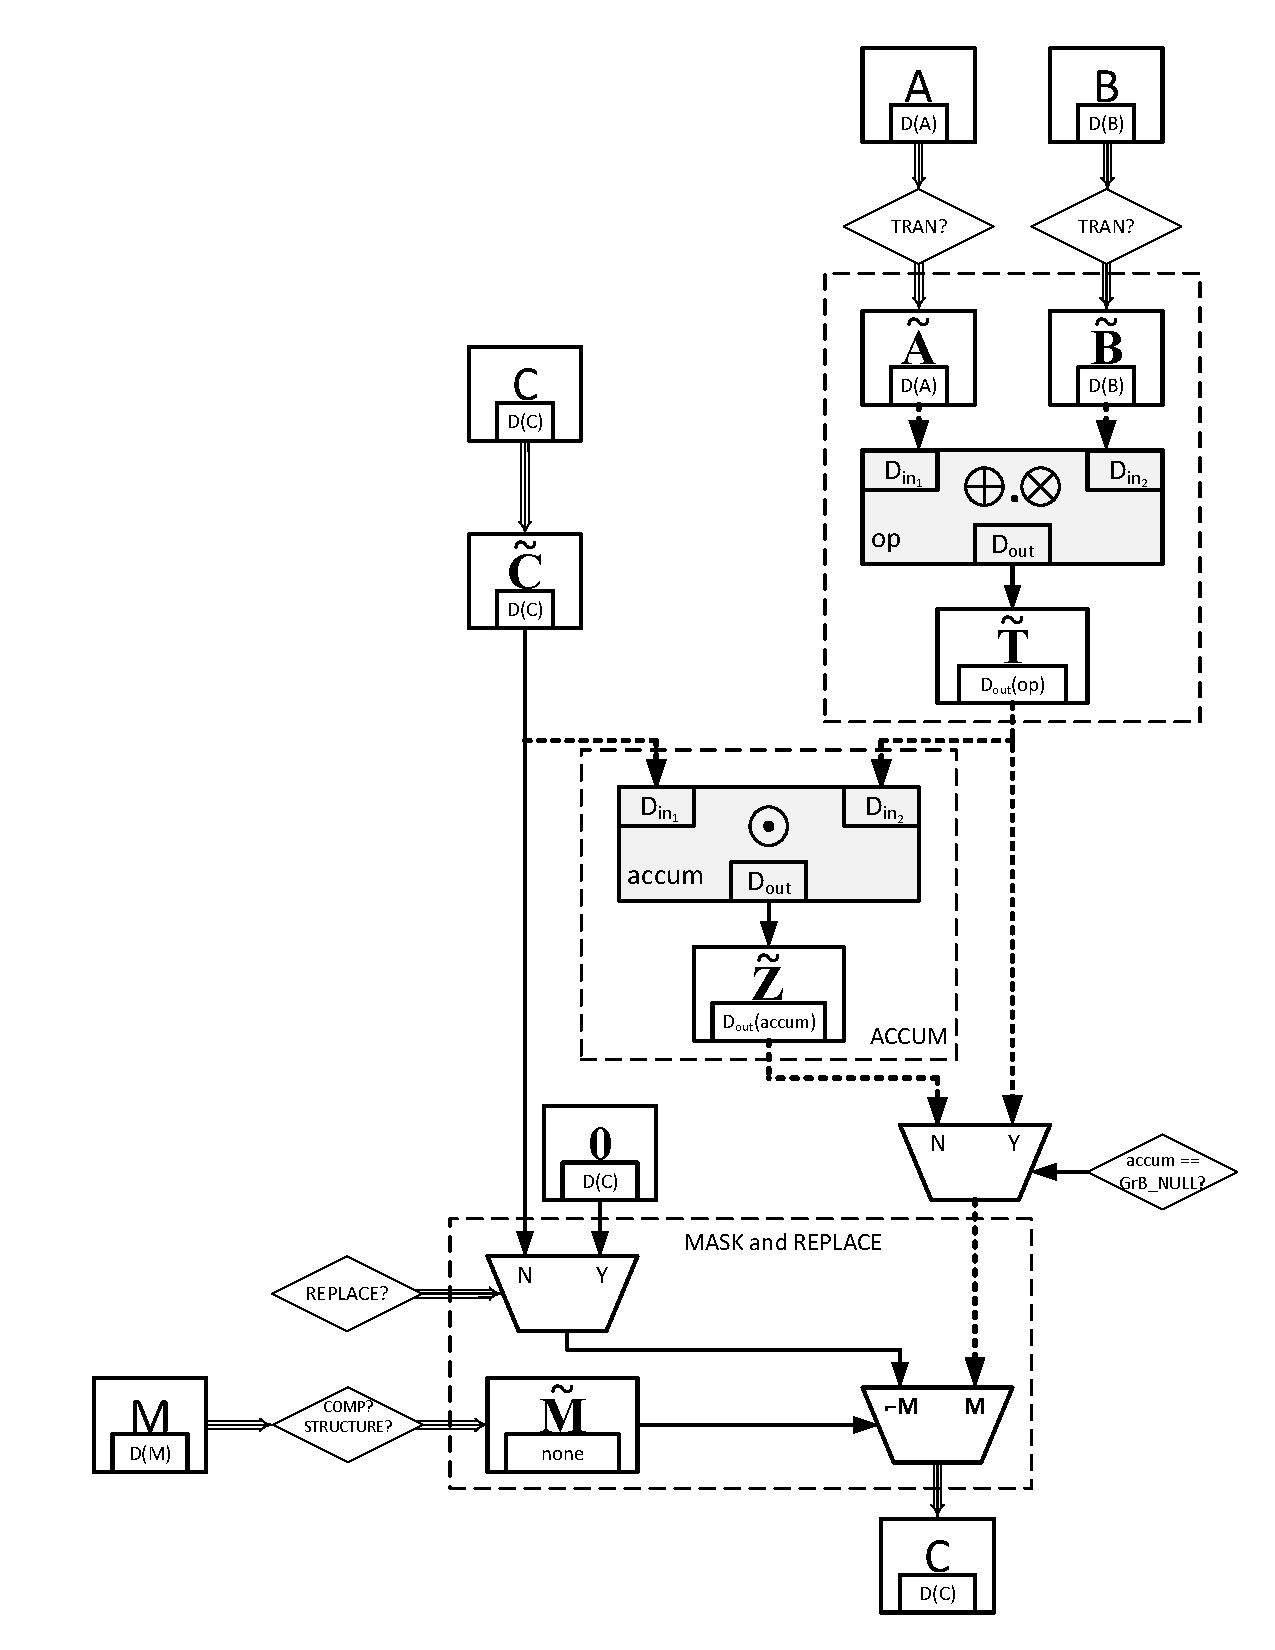
\includegraphics[width=5.5in]{mxm_operation_flowchart_1_3d.pdf}
    \end{center}
    \caption[Flowchart for the GraphBLAS operations.]{Flowchart for the GraphBLAS operations. Although shown specifically for
	the {\sf mxm} operation, many elements are common to all operations: such as the 
	``{\sf ACCUM}'' and ``{\sf MASK and REPLACE}'' blocks.  The triple arrows 
    ($\Rrightarrow$) denote where ``as if copy'' takes place (including both 
    collections and descriptor settings).  The bold, dotted arrows indicate
    where casting may occur between different domains.}
    \label{Fig:mxmFlowchart}
    \hrule
\end{figure}

\paragraph{Domains and Casting}

A GraphBLAS operation is only valid when the domains of the GraphBLAS objects are
mathematically consistent.  The C programming language defines implicit casts 
between built-in data types.  For example, {\sf float}s, {\sf double}s, and {\sf int}s can be 
freely mixed according to the rules defined for implicit casts.  It is the 
responsibility of the user to assure that these casts are appropriate for the 
algorithm in question.  For example, a cast to {\sf int} implies truncation of a floating 
point type.  Depending on the operation, this truncation error could lead to
erroneous results.  Furthermore, casting a wider type onto a narrower type can lead 
to overflow errors.  The GraphBLAS operations do not attempt to protect a user from 
these sorts of errors.

When user-define types are involved, however, GraphBLAS requires strict equivalence
between types and no casting is supported.  If GraphBLAS detects these mismatches,
it will return a domain mismatch error.

\paragraph{Dimensions and Transposes}

GraphBLAS operations also make assumptions about the numbers of dimensions and 
the sizes of vectors and matrices in an operation.   An operation will test these 
sizes and report an error if they are not \emph{shape compatible}.  For example, when multiplying 
two matrices, $\matrix{C} = \matrix{A} \times \matrix{B}$, the number of rows of 
$\matrix{C}$ must equal the number of rows of $\matrix{A}$, the number of columns 
of $\matrix{A}$ must match the number of rows of $\matrix{B}$, and the number of 
columns of $\matrix{C}$ must match the number of columns of $\matrix{B}$.  This 
is the behavior expected given the mathematical definition of the operations.   

For most of the GraphBLAS operations involving matrices, an optional descriptor 
can modify the matrix associated with an input GraphBLAS matrix object.  For 
example, if an input matrix is an argument to a GraphBLAS operation and the 
associated descriptor indicates the transpose option, then the operation occurs 
as if on the transposed matrix.  In this case, the relationships between the 
sizes in each dimension shift in the mathematically expected way. 

\paragraph{Masks: Structure-only, Complement, and Replace}

When a GraphBLAS operation supports the use of an optional mask, that mask is
specified through a GraphBLAS vector (for one-dimensional masks) or
a GraphBLAS matrix (for two-dimensional masks).  When a mask is used and the 
{\tt GrB\_STRUCTURE} descriptor value is not set, it is applied to the result 
from the operation wherever the stored values in the mask evaluate to true.  If
the {\tt GrB\_STRUCTURE} descriptor is set, the mask is applied to the result
from the operation wherever the mask as a stored value (regardless of that value).
Wherever the mask is applied, the result from the operation is either assigned 
to the provided output matrix/vector or, if a binary accumulation operation is 
provided, the result is accumulated into the corresponding elements of the provided 
output matrix/vector.

Given a GraphBLAS vector $\vector{v} = \langle D,N, \{ (i,v_i) \} \rangle$, a
one-dimensional mask is derived for use in the operation as follows:
\[
\vector{m} = 
\begin{cases}
\langle N, \{ \mathbf{ind}(\vector{v}) \} \rangle, & \mbox{if {\tt GrB\_STRUCTURE} is specified,} \\
\langle N, \{ i : \mbox{\tt (bool)}v_i = \true \} \rangle, & \mbox{otherwise}
\end{cases}
\]
where {\tt (bool)}$v_i$ denotes casting the value $v_i$ to a Boolean value (\true\ or \false).
Likewise, given a GraphBLAS matrix $\matrix{A} = \langle D, M, N, \{ (i,j,A_{ij}) \} \rangle$,
a two-dimensional mask is derived for use in the operation as follows:
\[
\matrix{M} = 
\begin{cases}
\langle M,N, \{ \mathbf{ind}(\matrix{A}) \} \rangle, & \mbox{if {\tt GrB\_STRUCTURE} is specified,} \\
\langle M,N, \{ (i,j) : \mbox{\tt (bool)}A_{ij} = \true \} \rangle, & \mbox{otherwise}
\end{cases}
\]
where {\tt (bool)}$A_{ij}$ denotes casting the value $A_{ij}$ to a Boolean value. 
(\true\ or \false)

In both the one- and two-dimensional cases, the mask may also have a subsequent 
complement operation applied ($Section$~\ref{Sec:Masks}) as specified in the 
descriptor, before a final mask is generated for use in the operation.

When the descriptor of an operation with a mask has specified that 
the {\sf GrB\_REPLACE} value is to be applied to the output ({\sf GrB\_OUTP}),
then anywhere the mask is not {\sf true}, the corresponding location in
the output is cleared.


\paragraph{Invalid and uninitialized objects}

Upon entering a GraphBLAS operation, the first step is a check that all
objects are valid and initialized. (Optional parameters can be set to {\sf
GrB\_NULL}, which always counts as a valid object.)  An invalid object is
one that could not be computed due to a previous execution error. An
unitialized object is one that has not yet been created by a corresponding
{\sf new} or {\sf dup} method.  Appropriate error codes are returned if
an object is not initialized ({\sf GrB\_UNINITIALIZED\_OBJECT}) or invalid
({\sf GrB\_INVALID\_OBJECT}).

To support the detection of as many cases of uninitialized objects as possible,
it is strongly recommended to initialize all GraphBLAS objects to
the predefined value {\sf GrB\_INVALID\_HANDLE} at the point of their declaration,
as shown in the following examples:

\begin{verbatim}
        GrB_Type        type = GrB_INVALID_HANDLE;
        GrB_Semiring    semiring = GrB_INVALID_HANDLE;
        GrB_Matrix      matrix = GrB_INVALID_HANDLE;
\end{verbatim}

\paragraph{Compliance}

We follow a \emph{prescriptive} approach to the definition of the semantics
of GraphBLAS operations. That is, for each operation we give a recipe for
producing its outcome.
Any implementation that produces the same outcome,
and follows the GraphBLAS execution model (Section~\ref{Sec:ExecutionModel}) and
error model (Section~\ref{Sec:ErrorModel}) is a conforming implementation.


%-----------------------------------------------------------------------------
\subsection{{\sf mxm}: Matrix-matrix multiply}

Multiplies a matrix with another matrix on a semiring. The result is a matrix.

\paragraph{\syntax}

\begin{verbatim}
        GrB_Info GrB_mxm(GrB_Matrix             C,
                         const GrB_Matrix       Mask,
                         const GrB_BinaryOp     accum,
                         const GrB_Semiring     op,
                         const GrB_Matrix       A,
                         const GrB_Matrix       B,
                         const GrB_Descriptor   desc);
\end{verbatim}

\paragraph{Parameters}

\begin{itemize}[leftmargin=1.1in]
    \item[{\sf C}]    ({\sf INOUT}) An existing GraphBLAS matrix. On input,
    the matrix provides values that may be accumulated with the result of the
    matrix product.  On output, the matrix holds the results of the
    operation.

    \item[{\sf Mask}] ({\sf IN}) An optional ``write'' mask that controls which
    results from this operation are stored into the output matrix {\sf C}. The 
    mask dimensions must match those of the matrix {\sf C}. If the 
    {\sf GrB\_STRUCTURE} descriptor is {\em not} set for the mask, the domain 
    of the {\sf Mask} matrix must be of type {\sf bool} or any of the predefined 
    ``built-in'' types in Table~\ref{Tab:PredefinedTypes}.  If the default
    mask is desired (\ie, a mask that is all {\sf true} with the dimensions of {\sf C}), 
    {\sf GrB\_NULL} should be specified.

    \item[{\sf accum}] ({\sf IN}) An optional binary operator used for accumulating
    entries into existing {\sf C} entries.
    %: ${\sf accum} = \langle \bDout({\sf accum}),\bDin1({\sf accum}),
    %\bDin2({\sf accum}), \odot \rangle$. 
    If assignment rather than accumulation is
    desired, {\sf GrB\_NULL} should be specified.

    \item[{\sf op}]   ({\sf IN}) The semiring used in the matrix-matrix
    multiply.
    %: ${\sf op}=\langle \bDout({\sf op}),\bDin1({\sf op}),\bDin2({\sf op}),\oplus,\otimes,0 \rangle$.

    \item[{\sf A}]    ({\sf IN}) The GraphBLAS matrix holding the values
    for the left-hand matrix in the multiplication.

    \item[{\sf B}]    ({\sf IN}) The GraphBLAS matrix holding the values for
    the right-hand matrix in the multiplication.

    \item[{\sf desc}] ({\sf IN}) An optional operation descriptor. If
    a \emph{default} descriptor is desired, {\sf GrB\_NULL} should be
    specified. Non-default field/value pairs are listed as follows:  \\
    
    \hspace*{-2em}\begin{tabular}{lllp{2.7in}}
        Param & Field  & Value & Description \\
        \hline
        {\sf C}    & {\sf GrB\_OUTP} & {\sf GrB\_REPLACE} & Output matrix {\sf C}
        is cleared (all elements removed) before the result is stored in it.\\

        {\sf Mask} & {\sf GrB\_MASK} & {\sf GrB\_STRUCTURE}   & The write mask is
        constructed from the structure (pattern of stored values) of the input
        {\sf Mask} matrix. The stored values are not examined.\\

        {\sf Mask} & {\sf GrB\_MASK} & {\sf GrB\_COMP}   & Use the
        complement of {\sf Mask}. \\

        {\sf A}    & {\sf GrB\_INP0} & {\sf GrB\_TRAN}   & Use transpose of {\sf A}
        for the operation. \\

        {\sf B}    & {\sf GrB\_INP1} & {\sf GrB\_TRAN}   & Use transpose of {\sf B}
        for the operation. \\
    \end{tabular}
\end{itemize}

\paragraph{Return Values}

\begin{itemize}[leftmargin=2.1in]
    \item[{\sf GrB\_SUCCESS}]         In blocking mode, the operation completed
    successfully. In non-blocking mode, this indicates that the compatibility 
    tests on dimensions and domains for the input arguments passed successfully. 
    Either way, output matrix {\sf C} is ready to be used in the next method of
    the sequence.

    \item[{\sf GrB\_PANIC}]           Unknown internal error.

    \item[{\sf GrB\_INVALID\_OBJECT}] This is returned in any execution mode 
    whenever one of the opaque GraphBLAS objects (input or output) is in an invalid 
    state caused by a previous execution error.  Call {\sf GrB\_error()} to access 
    any error messages generated by the implementation.

    \item[{\sf GrB\_OUT\_OF\_MEMORY}] Not enough memory available for the operation.

    \item[{\sf GrB\_UNINITIALIZED\_OBJECT}] One or more of the GraphBLAS objects 
    has not been initialized by a call to {\sf new} (or {\sf Matrix\_dup} for matrix
    parameters).

    \item[{\sf GrB\_DIMENSION\_MISMATCH}] Mask and/or matrix
    dimensions are incompatible.

    \item[{\sf GrB\_DOMAIN\_MISMATCH}]    The domains of the various matrices are
    incompatible with the corresponding domains of the semiring or
    accumulation operator, or the mask's domain is not compatible with {\sf bool}
    (in the case where {\sf desc[GrB\_MASK].GrB\_STRUCTURE} is not set).
\end{itemize}

\paragraph{Description}

{\sf GrB\_mxm} computes the matrix product ${\sf C} = {\sf
A} \oplus . \otimes {\sf B}$ or, if an optional binary accumulation
operator ($\odot$) is provided, ${\sf C} = {\sf C} \odot
\left({\sf A} \oplus . \otimes {\sf B}\right)$ (where matrices {\sf A}
and {\sf B} can be optionally transposed).  Logically, this operation
occurs in three steps:
\begin{enumerate}[leftmargin=0.85in]
\item[\bf Setup] The internal matrices and mask used in the computation are formed and their 
domains and dimensions are tested for compatibility.
\item[\bf Compute] The indicated computations are carried out.
\item[\bf Output] The result is written into the output matrix, possibly under control of a mask.
\end{enumerate}

Up to four argument matrices are used in the {\sf GrB\_mxm} operation:
\begin{enumerate}
	\item ${\sf C} = \langle \bold{D}({\sf C}),\bold{nrows}({\sf C}),\bold{ncols}({\sf C}),\bold{L}({\sf C}) = \{(i,j,C_{ij}) \} \rangle$
	\item ${\sf Mask} = \langle \bold{D}({\sf Mask}),\bold{nrows}({\sf Mask}),\bold{ncols}({\sf Mask}),\bold{L}({\sf Mask}) = \{(i,j,M_{ij}) \} \rangle$ (optional)
	\item ${\sf A} = \langle \bold{D}({\sf A}),\bold{nrows}({\sf A}), \bold{ncols}({\sf A}),\bold{L}({\sf A}) = \{(i,j,A_{ij}) \} \rangle$
	\item ${\sf B} = \langle \bold{D}({\sf B}),\bold{nrows}({\sf B}), \bold{ncols}({\sf B}),\bold{L}({\sf B}) = \{(i,j,B_{ij}) \} \rangle$
\end{enumerate}

The argument matrices, the semiring, and the accumulation operator (if provided) 
are tested for domain compatibility as follows:
\begin{enumerate}
	\item If {\sf Mask} is not {\sf GrB\_NULL}, and ${\sf desc[GrB\_MASK].GrB\_STRUCTURE}$
    is not set, then $\bold{D}({\sf Mask})$ must be from one of the pre-defined types of 
    Table~\ref{Tab:PredefinedTypes}.

	\item $\bold{D}({\sf A})$ must be compatible with $\bDin1({\sf op})$ of the semiring.

	\item $\bold{D}({\sf B})$ must be compatible with $\bDin2({\sf op})$ of the semiring.

	\item $\bold{D}({\sf C})$ must be compatible with $\bDout({\sf op})$ of the semiring.

	\item If {\sf accum} is not {\sf GrB\_NULL}, then $\bold{D}({\sf C})$ must be
    compatible with $\bDin1({\sf accum})$ and $\bDout({\sf accum})$ of the 
    accumulation operator and $\bDout({\sf op})$ of the semiring must be compatible with 
    $\bDin2({\sf accum})$ of the accumulation operator.
\end{enumerate}
Two domains are compatible with each other if values from one domain can be cast 
to values in the other domain as per the rules of the C language.
In particular, domains from Table~\ref{Tab:PredefinedTypes} are all compatible 
with each other. A domain from a user-defined type is only compatible with itself.
If any compatibility rule above is violated, execution of {\sf GrB\_mxm} ends and 
the domain mismatch error listed above is returned.

From the argument matrices, the internal matrices and mask used in 
the computation are formed ($\leftarrow$ denotes copy):
\begin{enumerate}
	\item Matrix $\matrix{\widetilde{C}} \leftarrow {\sf C}$.

	\item Two-dimensional mask, $\matrix{\widetilde{M}}$, is computed from
    argument {\sf Mask} as follows:
	\begin{enumerate}
		\item If ${\sf Mask} = {\sf GrB\_NULL}$, then $\matrix{\widetilde{M}} = 
        \langle \bold{nrows}({\sf C}), \bold{ncols}({\sf C}), \{(i,j), 
        \forall i,j : 0 \leq i <  \bold{nrows}({\sf C}), 0 \leq j < 
        \bold{ncols}({\sf C}) \} \rangle$.

		\item If {\sf Mask} $\ne$ {\sf GrB\_NULL},
        \begin{enumerate}
            \item If ${\sf desc[GrB\_MASK].GrB\_STRUCTURE}$ is set, then 
            $\matrix{\widetilde{M}} = \langle \bold{nrows}({\sf Mask}), 
            \bold{ncols}({\sf Mask}), \{(i,j) : (i,j) \in \bold{ind}({\sf Mask}) \} \rangle$,
            \item Otherwise, $\matrix{\widetilde{M}} = \langle \bold{nrows}({\sf Mask}), 
            \bold{ncols}({\sf Mask}), \\ \{(i,j) : (i,j) \in \bold{ind}({\sf Mask}) \wedge 
            ({\sf bool}){\sf Mask}(i,j) = \true\} \rangle$.
        \end{enumerate}

		\item	If ${\sf desc[GrB\_MASK].GrB\_COMP}$ is set, then 
        $\matrix{\widetilde{M}} \leftarrow \neg \matrix{\widetilde{M}}$.
	\end{enumerate}

	\item Matrix $\matrix{\widetilde{A}} \leftarrow
    {\sf desc[GrB\_INP0].GrB\_TRAN} \ ? \ {\sf A}^T : {\sf A}$.

	\item Matrix $\matrix{\widetilde{B}} \leftarrow
    {\sf desc[GrB\_INP1].GrB\_TRAN} \ ? \ {\sf B}^T : {\sf B}$.
\end{enumerate}

The internal matrices and masks are checked for dimension compatibility. The following
conditions must hold:
\begin{enumerate}
	\item $\bold{nrows}(\matrix{\widetilde{C}}) = \bold{nrows}(\matrix{\widetilde{M}})$.

	\item $\bold{ncols}(\matrix{\widetilde{C}}) = \bold{ncols}(\matrix{\widetilde{M}})$.

	\item $\bold{nrows}(\matrix{\widetilde{C}}) = \bold{nrows}(\matrix{\widetilde{A}})$.

	\item $\bold{ncols}(\matrix{\widetilde{C}}) = \bold{ncols}(\matrix{\widetilde{B}})$.

	\item $\bold{ncols}(\matrix{\widetilde{A}}) = \bold{nrows}(\matrix{\widetilde{B}})$.
\end{enumerate}
If any compatibility rule above is violated, execution of {\sf GrB\_mxm} ends and
the dimension mismatch error listed above is returned.

From this point forward, in {\sf GrB\_NONBLOCKING} mode, the method can 
optionally exit with {\sf GrB\_SUCCESS} return code and defer any computation 
and/or execution error codes.

We are now ready to carry out the matrix multiplication and any additional 
associated operations.  We describe this in terms of two intermediate matrices:
\begin{itemize}
    \item $\matrix{\widetilde{T}}$: The matrix holding the product of matrices 
    $\matrix{\widetilde{A}}$ and $\matrix{\widetilde{B}}$.
    \item $\matrix{\widetilde{Z}}$: The matrix holding the result after 
    application of the (optional) accumulation operator.
\end{itemize}

The intermediate matrix $\matrix{\widetilde{T}} = \langle
\bDout({\sf op}), \bold{nrows}(\matrix{\widetilde{A}}), \bold{ncols}(\matrix{\widetilde{B}}),
\{(i,j,T_{ij}) : \bold{ind}(\matrix{\widetilde{A}}(i,:)) \cap
\bold{ind}(\matrix{\widetilde{B}}(:,j)) \neq \emptyset \} \rangle$
is created.  The value of each of its elements is computed by 
\[T_{ij} = \bigoplus_{k \in \bold{ind}(\matrix{\widetilde{A}}(i,:)) \cap
\bold{ind}(\matrix{\widetilde{B}}(:,j))} (\matrix{\widetilde{A}}(i,k)
\otimes \matrix{\widetilde{B}}(k,j)),\] where $\oplus$ and $\otimes$
are the additive and multiplicative operators of semiring {\sf op},
respectively.


The intermediate matrix $\matrix{\widetilde{Z}}$ is created as follows, using what is called a \emph{standard matrix accumulate}:
\begin{itemize}
    \item If ${\sf accum} = {\sf GrB\_NULL}$, then $\matrix{\widetilde{Z}} = \matrix{\widetilde{T}}$.

    \item If ${\sf accum}$ is a binary operator, then $\matrix{\widetilde{Z}}$ is defined as
        \[ \matrix{\widetilde{Z}} = \langle \bDout({\sf accum}), \bold{nrows}(\matrix{\widetilde{C}}), \bold{ncols}(\matrix{\widetilde{C}}),
        %\bold{L}(\matrix{\widetilde{Z}}) =
        \{(i,j,Z_{ij})  \forall (i,j) \in \bold{ind}(\matrix{\widetilde{C}}) \cup 
        \bold{ind}(\matrix{\widetilde{T}}) \} \rangle.\]

    The values of the elements of $\matrix{\widetilde{Z}}$ are computed based on the
    relationships between the sets of indices in $\matrix{\widetilde{C}}$ and 
    $\matrix{\widetilde{T}}$.
\[
    Z_{ij} = \matrix{\widetilde{C}}(i,j) \odot \matrix{\widetilde{T}}(i,j), \ \mbox{if}\  
    (i,j) \in  (\bold{ind}(\matrix{\widetilde{T}}) \cap \bold{ind}(\matrix{\widetilde{C}})),
\]
\[
    Z_{ij} = \matrix{\widetilde{C}}(i,j), \ \mbox{if}\  
    (i,j) \in (\bold{ind}(\matrix{\widetilde{C}}) - (\bold{ind}(\matrix{\widetilde{T}})
    \cap \bold{ind}(\matrix{\widetilde{C}}))),
\]
\[
    Z_{ij} = \matrix{\widetilde{T}}(i,j), \ \mbox{if}\  (i,j) \in  
    (\bold{ind}(\matrix{\widetilde{T}}) - (\bold{ind}(\matrix{\widetilde{T}})
    \cap \bold{ind}(\matrix{\widetilde{C}}))),
\]
where $\odot  = \bigodot({\sf accum})$, and the difference operator refers to set difference.
\end{itemize}



Finally, the set of output values that make up matrix $\matrix{\widetilde{Z}}$ 
are written into the final result matrix {\sf C}, using what is called
a \emph{standard matrix mask and replace}. 
This is carried out under control of the mask which acts as a ``write mask''.
\begin{itemize}
\item If {\sf desc[GrB\_OUTP].GrB\_REPLACE} is set, then any values in {\sf C} on
input to this operation are deleted and the content of the new output matrix,
{\sf C}, is defined as,
\[
\bold{L}({\sf C}) = \{(i,j,Z_{ij}) : (i,j) \in (\bold{ind}(\matrix{\widetilde{Z}}) 
\cap \bold{ind}(\matrix{\widetilde{M}})) \}. 
\]

\item If {\sf desc[GrB\_OUTP].GrB\_REPLACE} is not set, the elements of 
$\matrix{\widetilde{Z}}$ indicated by the mask are copied into the result 
matrix, {\sf C}, and elements of {\sf C} that fall outside the set 
indicated by the mask are unchanged:
\[
\bold{L}({\sf C}) = \{(i,j,C_{ij}) : (i,j) \in (\bold{ind}({\sf C}) 
\cap \bold{ind}(\neg \matrix{\widetilde{M}})) \} \cup \{(i,j,Z_{ij}) : (i,j) \in 
(\bold{ind}(\matrix{\widetilde{Z}}) \cap \bold{ind}(\matrix{\widetilde{M}})) \}.
\]
\end{itemize}

In {\sf GrB\_BLOCKING} mode, the method exits with return value 
{\sf GrB\_SUCCESS} and the new content of matrix {\sf C} is as defined above
and fully computed.
In {\sf GrB\_NONBLOCKING} mode, the method exits with return value 
{\sf GrB\_SUCCESS} and the new content of matrix {\sf C} is as defined above
but may not be fully computed. However, it can be used in the next GraphBLAS 
method call in a sequence.


%-----------------------------------------------------------------------------

\subsection{{\sf vxm}: Vector-matrix multiply}

Multiplies a (row) vector with a matrix on an semiring. The result is a vector.

\paragraph{\syntax}

\begin{verbatim}
        GrB_Info GrB_vxm(GrB_Vector             w,
                         const GrB_Vector       mask,
                         const GrB_BinaryOp     accum,
                         const GrB_Semiring     op,
                         const GrB_Vector       u, 
                         const GrB_Matrix       A,
                         const GrB_Descriptor   desc);
\end{verbatim}

\paragraph{Parameters}

\begin{itemize}[leftmargin=1.1in]
    \item[{\sf w}]    ({\sf INOUT}) An existing GraphBLAS vector.  On input,
    the vector provides values that may be accumulated with the result of the
    vector-matrix product.  On output, this vector holds the results of the
    operation.

    \item[{\sf mask}] ({\sf IN}) An optional ``write'' mask that controls which
    results from this operation are stored into the output vector {\sf w}. The 
    mask dimensions must match those of the vector {\sf w}. If the 
    {\sf GrB\_STRUCTURE} descriptor is {\em not} set for the mask, the domain of the
    {\sf mask} vector must be of type {\sf bool} or any of the predefined 
    ``built-in'' types in Table~\ref{Tab:PredefinedTypes}.  If the default
    mask is desired (\ie, a mask that is all {\sf true} with the dimensions of {\sf w}), 
    {\sf GrB\_NULL} should be specified.

    \item[{\sf accum}] ({\sf IN}) An optional binary operator used for accumulating
    entries into existing {\sf w} entries.
    %: ${\sf accum} = \langle \bDout({\sf accum}),\bDin1({\sf accum}),
    %\bDin2({\sf accum}), \odot \rangle$. 
    If assignment rather than accumulation is
    desired, {\sf GrB\_NULL} should be specified.

    \item[{\sf op}]   ({\sf IN}) Semiring used in the vector-matrix
    multiply.
    %: ${\sf op}=\langle \bDout({\sf op}),\bDin1({\sf op}),\bDin2({\sf op}),\oplus,\otimes,0 \rangle$.

    \item[{\sf u}]    ({\sf IN}) The GraphBLAS vector holding the values for
    the left-hand vector in the multiplication.

    \item[{\sf A}]    ({\sf IN}) The GraphBLAS matrix holding the values
    for the right-hand matrix in the multiplication.

    \item[{\sf desc}] ({\sf IN}) An optional operation descriptor. If
    a \emph{default} descriptor is desired, {\sf GrB\_NULL} should be
    specified. Non-default field/value pairs are listed as follows:  \\

    \hspace*{-2em}\begin{tabular}{lllp{2.7in}}
        Param & Field  & Value & Description \\
        \hline
        {\sf w}    & {\sf GrB\_OUTP} & {\sf GrB\_REPLACE} & Output vector {\sf w}
        is cleared (all elements removed) before the result is stored in it.\\

        {\sf mask} & {\sf GrB\_MASK} & {\sf GrB\_STRUCTURE}   & The write mask is
        constructed from the structure (pattern of stored values) of the input
        {\sf mask} vector. The stored values are not examined.\\

        {\sf mask} & {\sf GrB\_MASK} & {\sf GrB\_COMP}   & Use the
        complement of {\sf mask}. \\

        {\sf A}    & {\sf GrB\_INP1} & {\sf GrB\_TRAN}   & Use transpose of {\sf A}
        for the operation. \\
    \end{tabular}
\end{itemize}

\paragraph{Return Values}

\begin{itemize}[leftmargin=2.1in]
    \item[{\sf GrB\_SUCCESS}]         In blocking mode, the operation completed
    successfully. In non-blocking mode, this indicates that the compatibility 
    tests on dimensions and domains for the input arguments passed successfully. 
    Either way, output vector {\sf w} is ready to be used in the next method of 
    the sequence.

    \item[{\sf GrB\_PANIC}]           Unknown internal error.

    \item[{\sf GrB\_INVALID\_OBJECT}] This is returned in any execution mode 
    whenever one of the opaque GraphBLAS objects (input or output) is in an invalid 
    state caused by a previous execution error.  Call {\sf GrB\_error()} to access 
    any error messages generated by the implementation.

    \item[{\sf GrB\_OUT\_OF\_MEMORY}] Not enough memory available for the operation.

    \item[{\sf GrB\_UNINITIALIZED\_OBJECT}] One or more of the GraphBLAS objects 
    has not been initialized by a call to {\sf new} (or {\sf dup} for matrix or
    vector parameters).

    \item[{\sf GrB\_DIMENSION\_MISMATCH}] Mask, vector, and/or matrix 
    dimensions are incompatible.

    \item[{\sf GrB\_DOMAIN\_MISMATCH}]    The domains of the various vectors/matrices are
    incompatible with the corresponding domains of the semiring or
    accumulation operator, or the mask's domain is not compatible with {\sf bool}
    (in the case where {\sf desc[GrB\_MASK].GrB\_STRUCTURE} is not set).
\end{itemize}

\paragraph{Description}

{\sf GrB\_vxm} computes the vector-matrix product ${\sf w}^T = {\sf
u}^T \oplus . \otimes {\sf A}$, or, if an optional binary accumulation
operator ($\odot$) is provided, ${\sf w}^T = {\sf w}^T \odot
\left({\sf u}^T \oplus . \otimes {\sf A}\right)$ (where matrix {\sf A}
 can be optionally transposed).  Logically, this operation
occurs in three steps:
\begin{enumerate}[leftmargin=0.85in]
\item[\bf Setup] The internal vectors, matrices and mask used in the computation are formed and their domains/dimensions are tested for compatibility.
\item[\bf Compute] The indicated computations are carried out.
\item[\bf Output] The result is written into the output vector, possibly under control of a mask.
\end{enumerate}

Up to four argument vectors or matrices are used in the {\sf GrB\_vxm} operation:
\begin{enumerate}
	\item ${\sf w} = \langle \bold{D}({\sf w}),\bold{size}({\sf w}),\bold{L}({\sf w}) = \{(i,w_i) \} \rangle$
	\item ${\sf mask} = \langle \bold{D}({\sf mask}),\bold{size}({\sf mask}),\bold{L}({\sf mask}) = \{(i,m_i) \} \rangle$ (optional)
	\item ${\sf u} = \langle \bold{D}({\sf u}),\bold{size}({\sf u}),\bold{L}({\sf u}) = \{(i,u_i) \} \rangle$
	\item ${\sf A} = \langle \bold{D}({\sf A}),\bold{nrows}({\sf A}), \bold{ncols}({\sf A}),\bold{L}({\sf A}) = \{(i,j,A_{ij}) \} \rangle$
\end{enumerate}

The argument matrices, vectors, the semiring, and the accumulation operator (if provided) 
are tested for domain compatibility as follows:
\begin{enumerate}
	\item If {\sf mask} is not {\sf GrB\_NULL}, and ${\sf desc[GrB\_MASK].GrB\_STRUCTURE}$
    is not set, then $\bold{D}({\sf mask})$ must be from one of the pre-defined types of 
    Table~\ref{Tab:PredefinedTypes}.

	\item $\bold{D}({\sf u})$ must be compatible with $\bDin1({\sf op})$ of the semiring.

	\item $\bold{D}({\sf A})$ must be compatible with $\bDin2({\sf op})$ of the semiring.

	\item $\bold{D}({\sf w})$ must be compatible with $\bDout({\sf op})$ of the semiring.

	\item If {\sf accum} is not {\sf GrB\_NULL}, then $\bold{D}({\sf w})$ must be compatible with $\bDin1({\sf accum})$ and $\bDout({\sf accum})$ of the 
	accumulation operator and $\bDout({\sf op})$ of the semiring must be compatible with $\bDin2({\sf accum})$ of the accumulation operator.
\end{enumerate}
Two domains are compatible with each other if values from one domain can be cast 
to values in the other domain as per the rules of the C language.
In particular, domains from Table~\ref{Tab:PredefinedTypes} are all compatible 
with each other. A domain from a user-defined type is only compatible with itself.
If any compatibility rule above is violated, execution of {\sf GrB\_vxm} ends and 
the domain mismatch error listed above is returned.

From the argument vectors and matrices, the internal matrices and mask used in 
the computation are formed ($\leftarrow$ denotes copy):
\begin{enumerate}
	\item Vector $\vector{\widetilde{w}} \leftarrow {\sf w}$.

	\item One-dimensional mask, $\vector{\widetilde{m}}$, is computed from 
    argument {\sf mask} as follows:
	\begin{enumerate}
		\item If ${\sf mask} = {\sf GrB\_NULL}$, then $\vector{\widetilde{m}} = 
        \langle \bold{size}({\sf w}), \{i, \ \forall \ i : 0 \leq i < 
        \bold{size}({\sf w}) \} \rangle$.

		\item If {\sf mask} $\ne$ {\sf GrB\_NULL},  
        \begin{enumerate}
            \item If ${\sf desc[GrB\_MASK].GrB\_STRUCTURE}$ is set, then
            $\vector{\widetilde{m}} = 
            \langle \bold{size}({\sf mask}), \{i : i \in \bold{ind}({\sf mask}) \} \rangle$,
            \item Otherwise, $\vector{\widetilde{m}} = 
            \langle \bold{size}({\sf mask}), \{i : i \in \bold{ind}({\sf mask}) \wedge
            ({\sf bool}){\sf mask}(i) = \true \} \rangle$.
        \end{enumerate}

		\item	If ${\sf desc[GrB\_MASK].GrB\_COMP}$ is set, then 
        $\vector{\widetilde{m}} \leftarrow \neg \vector{\widetilde{m}}$.
	\end{enumerate}

	\item Vector $\vector{\widetilde{u}} \leftarrow {\sf u}$.

	\item Matrix $\matrix{\widetilde{A}} \leftarrow {\sf desc[GrB\_INP1].GrB\_TRAN} \ ? \ {\sf A}^T : {\sf A}$.
\end{enumerate}

The internal matrices and masks are checked for shape compatibility. The following 
conditions must hold:
\begin{enumerate}
	\item $\bold{size}(\vector{\widetilde{w}}) = \bold{size}(\vector{\widetilde{m}})$.

	\item $\bold{size}(\vector{\widetilde{w}}) = \bold{ncols}(\matrix{\widetilde{A}})$.

	\item $\bold{size}(\vector{\widetilde{u}}) = \bold{nrows}(\matrix{\widetilde{A}})$.
\end{enumerate}
If any compatibility rule above is violated, execution of {\sf GrB\_vxm} ends and 
the dimension mismatch error listed above is returned.

From this point forward, in {\sf GrB\_NONBLOCKING} mode, the method can 
optionally exit with {\sf GrB\_SUCCESS} return code and defer any computation 
and/or execution error codes.

We are now ready to carry out the vector-matrix multiplication and any additional 
associated operations.  We describe this in terms of two intermediate vectors:
\begin{itemize}
    \item $\vector{\widetilde{t}}$: The vector holding the product of vector
    $\vector{\widetilde{u}}^T$ and matrix $\matrix{\widetilde{A}}$.
    \item $\vector{\widetilde{z}}$: The vector holding the result after 
    application of the (optional) accumulation operator.
\end{itemize}

The intermediate vector $\vector{\widetilde{t}} = \langle
\bDout({\sf op}), \bold{ncols}(\matrix{\widetilde{A}}),
\{(j,t_j) : \bold{ind}(\vector{\widetilde{u}}) \cap
\bold{ind}(\matrix{\widetilde{A}}(:,j)) \neq \emptyset \} \rangle$
is created.  The value of each of its elements is computed by 
\[t_j = \bigoplus_{k \in \bold{ind}(\vector{\widetilde{u}}) \cap
\bold{ind}(\matrix{\widetilde{A}}(:,j))} (\vector{\widetilde{u}}(k)
\otimes \matrix{\widetilde{A}}(k,j)),\] where $\oplus$ and $\otimes$
are the additive and multiplicative operators of semiring {\sf op},
respectively.


The intermediate vector $\vector{\widetilde{z}}$ is created as follows, using what is called a \emph{standard vector accumulate}:
\begin{itemize}
    \item If ${\sf accum} = {\sf GrB\_NULL}$, then $\vector{\widetilde{z}} = \vector{\widetilde{t}}$.

    \item If ${\sf accum}$ is a binary operator, then $\vector{\widetilde{z}}$ is defined as
        \[ \vector{\widetilde{z}} = \langle \bDout({\sf accum}), \bold{size}(\vector{\widetilde{w}}),
        %\bold{L}(\vector{\widetilde{z}}) =
        \{(i,z_{i}) \ \forall \ i \in \bold{ind}(\vector{\widetilde{w}}) \cup 
        \bold{ind}(\vector{\widetilde{t}}) \} \rangle.\]

    The values of the elements of $\vector{\widetilde{z}}$ are computed based on the 
    relationships between the sets of indices in $\vector{\widetilde{w}}$ and 
    $\vector{\widetilde{t}}$.
\[
    z_{i} = \vector{\widetilde{w}}(i) \odot \vector{\widetilde{t}}(i), \ \mbox{if}\  
    i \in  (\bold{ind}(\vector{\widetilde{t}}) \cap \bold{ind}(\vector{\widetilde{w}})),
\]
\[
    z_{i} = \vector{\widetilde{w}}(i), \ \mbox{if}\  
    i \in (\bold{ind}(\vector{\widetilde{w}}) - (\bold{ind}(\vector{\widetilde{t}})
    \cap \bold{ind}(\vector{\widetilde{w}}))),
\]
\[
    z_{i} = \vector{\widetilde{t}}(i), \ \mbox{if}\  i \in  
    (\bold{ind}(\vector{\widetilde{t}}) - (\bold{ind}(\vector{\widetilde{t}})
    \cap \bold{ind}(\vector{\widetilde{w}}))),
\]
where $\odot  = \bigodot({\sf accum})$, and the difference operator refers to set difference.
\end{itemize}




Finally, the set of output values that make up vector $\vector{\widetilde{z}}$ 
are written into the final result vector {\sf w}, using
what is called a \emph{standard vector mask and replace}. 
This is carried out under control of the mask which acts as a ``write mask''.
\begin{itemize}
\item If {\sf desc[GrB\_OUTP].GrB\_REPLACE} is set, then any values in {\sf w} 
on input to this operation are deleted and the content of the new output vector,
{\sf w}, is defined as,
\[ 
\bold{L}({\sf w}) = \{(i,z_{i}) : i \in (\bold{ind}(\vector{\widetilde{z}}) 
\cap \bold{ind}(\vector{\widetilde{m}})) \}. 
\]

\item If {\sf desc[GrB\_OUTP].GrB\_REPLACE} is not set, the elements of 
$\vector{\widetilde{z}}$ indicated by the mask are copied into the result 
vector, {\sf w}, and elements of {\sf w} that fall outside the set indicated by 
the mask are unchanged:
\[ 
\bold{L}({\sf w}) = \{(i,w_{i}) : i \in (\bold{ind}({\sf w}) 
\cap \bold{ind}(\neg \vector{\widetilde{m}})) \} \cup \{(i,z_{i}) : i \in 
(\bold{ind}(\vector{\widetilde{z}}) \cap \bold{ind}(\vector{\widetilde{m}})) \}. 
\]
\end{itemize}

In {\sf GrB\_BLOCKING} mode, the method exits with return value 
{\sf GrB\_SUCCESS} and the new content of vector {\sf w} is as defined above
and fully computed.  
In {\sf GrB\_NONBLOCKING} mode, the method exits with return value 
{\sf GrB\_SUCCESS} and the new content of vector {\sf w} is as defined above 
but may not be fully computed. However, it can be used in the next GraphBLAS 
method call in a sequence.


%-----------------------------------------------------------------------------

\subsection{{\sf mxv}: Matrix-vector multiply}

Multiplies a matrix by a vector on a semiring. The result is a vector.

\paragraph{\syntax}

\begin{verbatim}
        GrB_Info GrB_mxv(GrB_Vector             w,
                         const GrB_Vector       mask,
                         const GrB_BinaryOp     accum,
                         const GrB_Semiring     op,
                         const GrB_Matrix       A,
                         const GrB_Vector       u,
                         const GrB_Descriptor   desc);
\end{verbatim}

\paragraph{Parameters}

\begin{itemize}[leftmargin=1.1in]
    \item[{\sf w}]    ({\sf INOUT}) An existing GraphBLAS vector.  On input,
    the vector provides values that may be accumulated with the result of the
    matrix-vector product.  On output, this vector holds the results of the
    operation.

    \item[{\sf mask}] ({\sf IN}) An optional ``write'' mask that controls which
    results from this operation are stored into the output vector {\sf w}. The 
    mask dimensions must match those of the vector {\sf w}. If the 
    {\sf GrB\_STRUCTURE} descriptor is {\em not} set for the mask, the domain of the
    {\sf mask} vector must be of type {\sf bool} or any of the predefined 
    ``built-in'' types in Table~\ref{Tab:PredefinedTypes}.  If the default
    mask is desired (\ie, a mask that is all {\sf true} with the dimensions of {\sf w}), 
    {\sf GrB\_NULL} should be specified.

    \item[{\sf accum}] ({\sf IN}) An optional binary operator used for accumulating
    entries into existing {\sf w} entries.
    %: ${\sf accum} = \langle \bDout({\sf accum}),\bDin1({\sf accum}),
    %\bDin2({\sf accum}), \odot \rangle$. 
    If assignment rather than accumulation is
    desired, {\sf GrB\_NULL} should be specified.

    \item[{\sf op}]   ({\sf IN}) Semiring used in the vector-matrix
    multiply.
    %: ${\sf op}=\langle \bDout({\sf op}),\bDin1({\sf op}),\bDin2({\sf op}),\oplus,\otimes,0 \rangle$.

    \item[{\sf A}]    ({\sf IN}) The GraphBLAS matrix holding the values
    for the left-hand matrix in the multiplication.

    \item[{\sf u}]    ({\sf IN}) The GraphBLAS vector holding the values for
    the right-hand vector in the multiplication.

    \item[{\sf desc}] ({\sf IN}) An optional operation descriptor. If
    a \emph{default} descriptor is desired, {\sf GrB\_NULL} should be
    specified. Non-default field/value pairs are listed as follows:  \\

    \hspace*{-2em}\begin{tabular}{lllp{2.7in}}
        Param & Field  & Value & Description \\
        \hline
        {\sf w}    & {\sf GrB\_OUTP} & {\sf GrB\_REPLACE} & Output vector {\sf w}
        is cleared (all elements removed) before the result is stored in it.\\

        {\sf mask} & {\sf GrB\_MASK} & {\sf GrB\_STRUCTURE}   & The write mask is
        constructed from the structure (pattern of stored values) of the input
        {\sf mask} vector. The stored values are not examined.\\

        {\sf mask} & {\sf GrB\_MASK} & {\sf GrB\_COMP}   & Use the
        complement of {\sf mask}. \\

        {\sf A}    & {\sf GrB\_INP0} & {\sf GrB\_TRAN}   & Use transpose of {\sf A}
        for the operation. \\
    \end{tabular}
\end{itemize}

\paragraph{Return Values}

\begin{itemize}[leftmargin=2.1in]
    \item[{\sf GrB\_SUCCESS}]         In blocking mode, the operation completed
    successfully. In non-blocking mode, this indicates that the compatibility 
    tests on dimensions and domains for the input arguments passed successfully. 
    Either way, output vector {\sf w} is ready to be used in the next method of 
    the sequence.

    \item[{\sf GrB\_PANIC}]           Unknown internal error.

    \item[{\sf GrB\_INVALID\_OBJECT}] This is returned in any execution mode 
    whenever one of the opaque GraphBLAS objects (input or output) is in an invalid 
    state caused by a previous execution error.  Call {\sf GrB\_error()} to access 
    any error messages generated by the implementation.

    \item[{\sf GrB\_OUT\_OF\_MEMORY}] Not enough memory available for the operation.

    \item[{\sf GrB\_UNINITIALIZED\_OBJECT}] One or more of the GraphBLAS objects 
    has not been initialized by a call to {\sf new} (or {\sf dup} for matrix or
    vector parameters).

    \item[{\sf GrB\_DIMENSION\_MISMATCH}] Mask, vector, and/or matrix 
    dimensions are incompatible.

    \item[{\sf GrB\_DOMAIN\_MISMATCH}]    The domains of the various vectors/matrices are
    incompatible with the corresponding domains of the semiring or
    accumulation operator, or the mask's domain is not compatible with {\sf bool}
    (in the case where {\sf desc[GrB\_MASK].GrB\_STRUCTURE} is not set).
\end{itemize}

\paragraph{Description}

{\sf GrB\_mxv} computes the matrix-vector product ${\sf w} = {\sf A}
\oplus . \otimes {\sf u}$, or, if an optional binary accumulation
operator ($\odot$) is provided, ${\sf w} = {\sf w} \odot \left({\sf A}
\oplus . \otimes {\sf u}\right)$ (where matrix {\sf A}
 can be optionally transposed).  Logically, this operation
occurs in three steps:
\begin{enumerate}[leftmargin=0.85in]
\item[\bf Setup] The internal vectors, matrices and mask used in the computation are formed and their domains/dimensions are tested for compatibility.
\item[\bf Compute] The indicated computations are carried out.
\item[\bf Output] The result is written into the output vector, possibly under control of a mask.
\end{enumerate}

Up to four argument vectors or matrices are used in the {\sf GrB\_mxv} operation:
\begin{enumerate}
	\item ${\sf w} = \langle \bold{D}({\sf w}),\bold{size}({\sf w}),\bold{L}({\sf w}) = \{(i,w_i) \} \rangle$
	\item ${\sf mask} = \langle \bold{D}({\sf mask}),\bold{size}({\sf mask}),\bold{L}({\sf mask}) = \{(i,m_i) \} \rangle$ (optional)
	\item ${\sf A} = \langle \bold{D}({\sf A}),\bold{nrows}({\sf A}), \bold{ncols}({\sf A}),\bold{L}({\sf A}) = \{(i,j,A_{ij}) \} \rangle$
	\item ${\sf u} = \langle \bold{D}({\sf u}),\bold{size}({\sf u}),\bold{L}({\sf u}) = \{(i,u_i) \} \rangle$
\end{enumerate}

The argument matrices, vectors, the semiring, and the accumulation operator (if provided) 
are tested for domain compatibility as follows:
\begin{enumerate}
	\item If {\sf mask} is not {\sf GrB\_NULL}, and ${\sf desc[GrB\_MASK].GrB\_STRUCTURE}$
    is not set, then $\bold{D}({\sf mask})$ must be from one of the pre-defined types of 
    Table~\ref{Tab:PredefinedTypes}.

	\item $\bold{D}({\sf A})$ must be compatible with $\bDin1({\sf op})$ of the semiring.

	\item $\bold{D}({\sf u})$ must be compatible with $\bDin2({\sf op})$ of the semiring.

	\item $\bold{D}({\sf w})$ must be compatible with $\bDout({\sf op})$ of the semiring.

	\item If {\sf accum} is not {\sf GrB\_NULL}, then $\bold{D}({\sf w})$ must be compatible with $\bDin1({\sf accum})$ and $\bDout({\sf accum})$ of the 
	accumulation operator and $\bDout({\sf op})$ of the semiring must be compatible with $\bDin2({\sf accum})$ of the accumulation operator.
\end{enumerate}
Two domains are compatible with each other if values from one domain can be cast 
to values in the other domain as per the rules of the C language.
In particular, domains from Table~\ref{Tab:PredefinedTypes} are all compatible 
with each other. A domain from a user-defined type is only compatible with itself.
If any compatibility rule above is violated, execution of {\sf GrB\_mxv} ends and 
the domain mismatch error listed above is returned.

From the argument vectors and matrices, the internal matrices and mask used in 
the computation are formed ($\leftarrow$ denotes copy):
\begin{enumerate}
	\item Vector $\vector{\widetilde{w}} \leftarrow {\sf w}$.

	\item One-dimensional mask, $\vector{\widetilde{m}}$, is computed from 
    argument {\sf mask} as follows:
	\begin{enumerate}
		\item If ${\sf mask} = {\sf GrB\_NULL}$, then $\vector{\widetilde{m}} = 
        \langle \bold{size}({\sf w}), \{i, \ \forall \ i : 0 \leq i < 
        \bold{size}({\sf w}) \} \rangle$.

		\item If {\sf mask} $\ne$ {\sf GrB\_NULL},  
        \begin{enumerate}
            \item If ${\sf desc[GrB\_MASK].GrB\_STRUCTURE}$ is set, then
            $\vector{\widetilde{m}} = 
            \langle \bold{size}({\sf mask}), \{i : i \in \bold{ind}({\sf mask}) \} \rangle$,
            \item Otherwise, $\vector{\widetilde{m}} = 
            \langle \bold{size}({\sf mask}), \{i : i \in \bold{ind}({\sf mask}) \wedge
            ({\sf bool}){\sf mask}(i) = \true \} \rangle$.
        \end{enumerate}

		\item	If ${\sf desc[GrB\_MASK].GrB\_COMP}$ is set, then 
        $\vector{\widetilde{m}} \leftarrow \neg \vector{\widetilde{m}}$.
	\end{enumerate}

	\item Matrix $\matrix{\widetilde{A}} \leftarrow {\sf desc[GrB\_INP0].GrB\_TRAN} \ ? \ {\sf A}^T : {\sf A}$.

	\item Vector $\vector{\widetilde{u}} \leftarrow {\sf u}$.
\end{enumerate}

The internal matrices and masks are checked for shape compatibility. The following 
conditions must hold:
\begin{enumerate}
	\item $\bold{size}(\vector{\widetilde{w}}) = \bold{size}(\vector{\widetilde{m}})$.

	\item $\bold{size}(\vector{\widetilde{w}}) = \bold{nrows}(\matrix{\widetilde{A}})$.

	\item $\bold{size}(\vector{\widetilde{u}}) = \bold{ncols}(\matrix{\widetilde{A}})$.
\end{enumerate}
If any compatibility rule above is violated, execution of {\sf GrB\_mxv} ends and 
the dimension mismatch error listed above is returned.

From this point forward, in {\sf GrB\_NONBLOCKING} mode, the method can 
optionally exit with {\sf GrB\_SUCCESS} return code and defer any computation 
and/or execution error codes.

We are now ready to carry out the matrix-vector multiplication and any additional 
associated operations.  We describe this in terms of two intermediate vectors:
\begin{itemize}
    \item $\vector{\widetilde{t}}$: The vector holding the product of matrix 
    $\matrix{\widetilde{A}}$ and vector $\vector{\widetilde{u}}$.
    \item $\vector{\widetilde{z}}$: The vector holding the result after 
    application of the (optional) accumulation operator.
\end{itemize}

The intermediate vector $\vector{\widetilde{t}} = \langle
\bDout({\sf op}), \bold{nrows}(\matrix{\widetilde{A}}),
\{(i,t_i) : \bold{ind}(\matrix{\widetilde{A}}(i,:)) \cap 
\bold{ind}(\vector{\widetilde{u}}) \neq \emptyset \} \rangle$
is created.  The value of each of its elements is computed by 
\[t_i = \bigoplus_{k \in \bold{ind}(\matrix{\widetilde{A}}(i,:)) \cap
\bold{ind}(\vector{\widetilde{u}})} (\matrix{\widetilde{A}}(i,k)
\otimes \vector{\widetilde{u}}(k)),\] where $\oplus$ and $\otimes$
are the additive and multiplicative operators of semiring {\sf op},
respectively.


The intermediate vector $\vector{\widetilde{z}}$ is created as follows, using what is called a \emph{standard vector accumulate}:
\begin{itemize}
    \item If ${\sf accum} = {\sf GrB\_NULL}$, then $\vector{\widetilde{z}} = \vector{\widetilde{t}}$.

    \item If ${\sf accum}$ is a binary operator, then $\vector{\widetilde{z}}$ is defined as
        \[ \vector{\widetilde{z}} = \langle \bDout({\sf accum}), \bold{size}(\vector{\widetilde{w}}),
        %\bold{L}(\vector{\widetilde{z}}) =
        \{(i,z_{i}) \ \forall \ i \in \bold{ind}(\vector{\widetilde{w}}) \cup 
        \bold{ind}(\vector{\widetilde{t}}) \} \rangle.\]

    The values of the elements of $\vector{\widetilde{z}}$ are computed based on the 
    relationships between the sets of indices in $\vector{\widetilde{w}}$ and 
    $\vector{\widetilde{t}}$.
\[
    z_{i} = \vector{\widetilde{w}}(i) \odot \vector{\widetilde{t}}(i), \ \mbox{if}\  
    i \in  (\bold{ind}(\vector{\widetilde{t}}) \cap \bold{ind}(\vector{\widetilde{w}})),
\]
\[
    z_{i} = \vector{\widetilde{w}}(i), \ \mbox{if}\  
    i \in (\bold{ind}(\vector{\widetilde{w}}) - (\bold{ind}(\vector{\widetilde{t}})
    \cap \bold{ind}(\vector{\widetilde{w}}))),
\]
\[
    z_{i} = \vector{\widetilde{t}}(i), \ \mbox{if}\  i \in  
    (\bold{ind}(\vector{\widetilde{t}}) - (\bold{ind}(\vector{\widetilde{t}})
    \cap \bold{ind}(\vector{\widetilde{w}}))),
\]
where $\odot  = \bigodot({\sf accum})$, and the difference operator refers to set difference.
\end{itemize}




Finally, the set of output values that make up vector $\vector{\widetilde{z}}$ 
are written into the final result vector {\sf w}, using
what is called a \emph{standard vector mask and replace}. 
This is carried out under control of the mask which acts as a ``write mask''.
\begin{itemize}
\item If {\sf desc[GrB\_OUTP].GrB\_REPLACE} is set, then any values in {\sf w} 
on input to this operation are deleted and the content of the new output vector,
{\sf w}, is defined as,
\[ 
\bold{L}({\sf w}) = \{(i,z_{i}) : i \in (\bold{ind}(\vector{\widetilde{z}}) 
\cap \bold{ind}(\vector{\widetilde{m}})) \}. 
\]

\item If {\sf desc[GrB\_OUTP].GrB\_REPLACE} is not set, the elements of 
$\vector{\widetilde{z}}$ indicated by the mask are copied into the result 
vector, {\sf w}, and elements of {\sf w} that fall outside the set indicated by 
the mask are unchanged:
\[ 
\bold{L}({\sf w}) = \{(i,w_{i}) : i \in (\bold{ind}({\sf w}) 
\cap \bold{ind}(\neg \vector{\widetilde{m}})) \} \cup \{(i,z_{i}) : i \in 
(\bold{ind}(\vector{\widetilde{z}}) \cap \bold{ind}(\vector{\widetilde{m}})) \}. 
\]
\end{itemize}

In {\sf GrB\_BLOCKING} mode, the method exits with return value 
{\sf GrB\_SUCCESS} and the new content of vector {\sf w} is as defined above
and fully computed.  
In {\sf GrB\_NONBLOCKING} mode, the method exits with return value 
{\sf GrB\_SUCCESS} and the new content of vector {\sf w} is as defined above 
but may not be fully computed. However, it can be used in the next GraphBLAS 
method call in a sequence.


%-----------------------------------------------------------------------------
\section{Element-wise multiplication or intersection}

{\sf eWiseMult} returns an object whose indices are the ``intersection'' of 
the indices of the inputs. The operator is invoked when scalars from two 
operands are present.

%-----------------------------------------------------------------------------

\subsection{{\sf eWiseMult/Intersect}: Vector variant}

Perform element-wise (general) multiplication on the intersection of elements 
of two vectors, producing a third vector as result.

\paragraph{\syntax}

$$
\matrix{T} ~ = ~ \vector{u} \otimes \vector{v}
$$

where

\begin{itemize}[leftmargin=1.1in]
    \item[$\vector{u}$]    ({\sf IN}) $\in \mathbb{D}_{u}^{n}$

    \item[$\vector{v}$]    ({\sf IN}) $\in \mathbb{D}_{v}^{n}$

    \item[$\otimes$]   ({\sf IN}) binary operator to combine values, $\mathbb{D}_{in1} \times \mathbb{D}_{in2} \rightarrow \mathbb{D}_\otimes$.  It does not need to commutative or associative.

    \item[$\matrix{T}$]    ({\sf OUT}) $\in \mathbb{D}_\otimes^{n}$

\end{itemize}

\paragraph{Description}

This variant of {\sf eWiseMult} or {\sf Intersect} computes the element-wise ``product'' or 
``intersection'' of two vectors given a specified binary operator, 
$\otimes$: $\matrix{T} = \vector{u} \otimes \vector{v}$.  Assuming the domains of the
elements in the vectors and the domains expected by the operator are compatible
and the sizes of the vectors are the same.

From the argument vectors, the internal vectors used in 
the computation are formed ($\leftarrow$ denotes copy):
\begin{enumerate}
	\item Vector $\vector{\widetilde{u}} \leftarrow \vector{u}$.

	\item Vector $\vector{\widetilde{v}} \leftarrow \vector{v}$.
\end{enumerate}

We are now ready to carry out the element-wise ``product''.

The intermediate vector $\vector{\widetilde{t}} = \langle
\bDout({\sf op}), \bold{size}(\vector{\widetilde{u}}),
\{(i,t_i) : \bold{ind}(\vector{\widetilde{u}}) \cap 
\bold{ind}(\vector{\widetilde{v}})
 \neq \emptyset \} \rangle$
is created.  The value of each of its elements is computed by:
\[t_i = (\vector{\widetilde{u}}(i)
\otimes \vector{\widetilde{v}}(i)), \forall i \in 
(\bold{ind}(\vector{\widetilde{u}}) \cap 
\bold{ind}(\vector{\widetilde{v}}))\]

%-----------------------------------------------------------------------------

\subsection{{\sf eWiseMult/Intersect}: Matrix variant}

Perform element-wise (general) multiplication on the intersection of elements 
of two matrices, producing a third matrix as result.

\paragraph{\syntax}


$$
\matrix{T} ~ = ~ \matrix{A}^{[T]} \otimes \matrix{B}^{[T]}
$$

where

\begin{itemize}[leftmargin=1.1in]
    \item[$\matrix{A}^{[T]}$]    ({\sf IN}) $\in \mathbb{D}_{A}^{n\times m}$

    \item[$\matrix{B}^{[T]}$]    ({\sf IN}) $\in \mathbb{D}_{B}^{n\times m}$

    \item[$\otimes$]   ({\sf IN}) binary operator to combine values, $\mathbb{D}_{in1} \times \mathbb{D}_{in2} \rightarrow \mathbb{D}_\otimes$.  It does not need to commutative nor associative.

    \item[$\matrix{T}$]    ({\sf OUT}) $\in \mathbb{D}_\otimes^{n\times m}$
\end{itemize}


\paragraph{Description}

This variant of {\sf eWiseMult} or {\sf Intersect} computes the element-wise ``product'' of
two matrices: $\matrix{T} = \matrix{A} \otimes \matrix{B}$.  Assuming the domains of the
elements in the matrices and the domains expected by the operator are compatible
and the sizes of the matrices (after optional transposes) are the same.

From the argument matrices, the internal matrices used in 
the computation are formed ($\leftarrow$ denotes copy): \scott{Find a notation that does not refer to descriptors (descriptors is an implementation detail not math).}
\begin{enumerate}
	\item Matrix $\matrix{\widetilde{A}} \leftarrow
    {\sf desc[GrB\_INP0].GrB\_TRAN} \ ? \ \matrix{A}^T : \matrix{A}$.

	\item Matrix $\matrix{\widetilde{B}} \leftarrow
    {\sf desc[GrB\_INP1].GrB\_TRAN} \ ? \ \matrix{B}^T : \matrix{B}$.
\end{enumerate}

The intermediate matrix $\matrix{\widetilde{T}} = \langle
\bDout({\sf op}), \bold{nrows}(\matrix{\widetilde{A}}), \bold{ncols}(\matrix{\widetilde{A}}),
\{(i,j,T_{ij}) : \bold{ind}(\matrix{\widetilde{A}}) \cap 
\bold{ind}(\matrix{\widetilde{B}}) \neq \emptyset \} \rangle$
is created.  The value of each of its elements is computed by 
\[T_{ij} = (\matrix{\widetilde{A}}(i,j)
\otimes \matrix{\widetilde{B}}(i,j)), \forall (i,j) \in 
\bold{ind}(\matrix{\widetilde{A}}) \cap 
\bold{ind}(\matrix{\widetilde{B}})\]

%=============================================================================
%-----------------------------------------------------------------------------
\section{Element-wise addition or union}

{\sf eWiseAdd} returns an object whose set of indices are the ``union'' of the 
indices of the input operand. The operator is invoked when scalars from two 
operands are present (either stored in the matrix or in the optional variant: 
passed as the fill-in value).


%-----------------------------------------------------------------------------
\subsection{{\sf eWiseAdd/Union}: Vector variant}

Perform element-wise (general) addition on the elements of two vectors,
producing a third vector as result.

\paragraph{\syntax}

\begin{eqnarray*}
\matrix{T} & = & \vector{u} \oplus \vector{v} \\
\matrix{T} & = & \left\{ \vector{u}\cup u_0 \right\} \oplus \left\{ \vector{v} \cup v_0 \right\}  \mbox{~~~(providing missing values)}
\end{eqnarray*}

where

\begin{itemize}[leftmargin=1.1in]
    \item[$\vector{u}$]    ({\sf IN}) $\in \mathbb{D}_{u}^{n}$

    \item[$\vector{v}$]    ({\sf IN}) $\in \mathbb{D}_{v}^{n}$

    \item[$\oplus$]   ({\sf IN}) binary operator to combine values, $\mathbb{D}_{in1} \times \mathbb{D}_{in2} \rightarrow \mathbb{D}_\oplus$.  It does not need to commutative or associative.

    \item[$\matrix{T}$]    ({\sf OUT}) $\in \mathbb{D}_\oplus^{n}$

\end{itemize}

\paragraph{Description}

This variant of {\sf eWiseAdd} or {\sf Union} computes the element-wise ``sum'' or
``union'' of two vectors given the specified binary operator, $\oplus$: 
$\matrix{T} = \vector{u} \oplus \vector{v}$.  Assuming the domains of the
elements in the vectors and the domains expected by the operator are compatible
and the sizes of the vectors are the same.

From the argument vectors, the internal vectors used in 
the computation are formed ($\leftarrow$ denotes copy):
\begin{enumerate}
	\item Vector $\vector{\widetilde{u}} \leftarrow \vector{u}$.

	\item Vector $\vector{\widetilde{v}} \leftarrow \vector{v}$.
\end{enumerate}

We are now ready to carry out the element-wise ``sum''.

The intermediate vector $\vector{\widetilde{t}} = \langle
\bDout({\sf op}), \bold{size}(\vector{\widetilde{u}}),
\{(i,t_i) : \bold{ind}(\vector{\widetilde{u}}) \cup 
\bold{ind}(\vector{\widetilde{v}})
 \neq \emptyset \} \rangle$
is created.  The value of each of its elements is computed by:
\begin{eqnarray*}
t_i & = & 
\begin{cases}
 \vector{\widetilde{u}}(i) \oplus \vector{\widetilde{v}}(i), & \forall i \in (\bold{ind}(\vector{\widetilde{u}}) \cap \bold{ind}(\vector{\widetilde{v}}))\\
 \vector{\widetilde{u}}(i), & \forall i \in (\bold{ind}(\vector{\widetilde{u}}) - (\bold{ind}(\vector{\widetilde{u}}) \cap \bold{ind}(\vector{\widetilde{v}})))\\
  \vector{\widetilde{v}}(i), & \forall i \in (\bold{ind}(\vector{\widetilde{v}}) - (\bold{ind}(\vector{\widetilde{u}}) \cap \bold{ind}(\vector{\widetilde{v}})))
\end{cases}
\end{eqnarray*}
where the difference operator in the previous expressions refers to set difference.

In the case where $u_0$ and $v_0$ scalars are specified they are used when only
one of the vector operands has a stored value at a particular location (and the other does).  
The value of each of its elements is computed by:
\begin{eqnarray*}
t_i & = & 
\begin{cases}
 \vector{\widetilde{u}}(i) \oplus \vector{\widetilde{v}}(i), & \forall i \in (\bold{ind}(\vector{\widetilde{u}}) \cap \bold{ind}(\vector{\widetilde{v}}))\\
 \vector{\widetilde{u}}(i) {\color{red}~ \oplus ~ v_0}, & \forall i \in (\bold{ind}(\vector{\widetilde{u}}) - (\bold{ind}(\vector{\widetilde{u}}) \cap \bold{ind}(\vector{\widetilde{v}})))\\

 {\color{red} u_0 ~\oplus ~}\vector{\widetilde{v}}(i), & \forall i \in (\bold{ind}(\vector{\widetilde{v}}) - (\bold{ind}(\vector{\widetilde{u}}) \cap \bold{ind}(\vector{\widetilde{v}})))
\end{cases}
\end{eqnarray*}
where the difference operator in the previous expressions refers to set difference.


%-----------------------------------------------------------------------------

\subsection{{\sf eWiseAdd/Union}: Matrix variant}

Perform element-wise (general) addition on the elements of two matrices,
producing a third matrix as result.

\paragraph{\syntax}

\begin{eqnarray*}
\matrix{T} & = & \matrix{A}^{[T]} \oplus \matrix{B}^{[T]} \\
\matrix{T} & = & \left\{ \matrix{A}^{[T]}\cup a_0 \right\} \oplus \left\{ \matrix{B}^{[T]} \cup b_0 \right\}  \mbox{~~~(providing missing values)}
\end{eqnarray*}

where

\begin{itemize}[leftmargin=1.1in]
    \item[$\matrix{A}^{[T]}$]    ({\sf IN}) $\in \mathbb{D}_{A}^{n\times m}$

    \item[$\matrix{B}^{[T]}$]    ({\sf IN}) $\in \mathbb{D}_{B}^{n\times m}$

    \item[$\oplus$]   ({\sf IN}) binary operator to combine values, $\mathbb{D}_{in1} \times \mathbb{D}_{in2} \rightarrow \mathbb{D}_\oplus$.  It does not need to commutative or associative.

    \item[$\matrix{T}$]    ({\sf OUT}) $\in \mathbb{D}_\otimes^{n\times m}$
\end{itemize}

\paragraph{Description}

This variant of {\sf eWiseAdd} or {\sf Union} computes the element-wise ``sum'' or
``union'' of two matrices given the specified binary operator, $\oplus$: 
$\matrix{T} = {\sf A} \oplus {\sf B}$.  Assuming the domains of the
elements in the matrices and the domains expected by the operator are compatible
and the sizes of the matrices are the same.

From the argument matrices, the internal matrices used in 
the computation are formed ($\leftarrow$ denotes copy): \scott{Find a notation that does not refer to descriptors (descriptors is an implementation detail not math).}
\begin{enumerate}	\item Matrix $\matrix{\widetilde{A}} \leftarrow
    {\sf desc[GrB\_INP0].GrB\_TRAN} \ ? \ {\sf A}^T : {\sf A}$.

	\item Matrix $\matrix{\widetilde{B}} \leftarrow
    {\sf desc[GrB\_INP1].GrB\_TRAN} \ ? \ {\sf B}^T : {\sf B}$.
\end{enumerate}

The intermediate matrix $\matrix{\widetilde{T}} = \langle
\bDout({\sf op}), \bold{nrows}(\matrix{\widetilde{A}}), \bold{ncols}(\matrix{\widetilde{A}}),
\{(i,j,T_{ij}) : \bold{ind}(\matrix{\widetilde{A}}) \cup 
\bold{ind}(\matrix{\widetilde{B}}) \neq \emptyset \} \rangle$
is created.  The value of each of its elements is computed by :
\begin{eqnarray*}
T_{ij} & = & 
\begin{cases}
 (\matrix{\widetilde{A}}(i,j) \oplus \matrix{\widetilde{B}}(i,j)),& \forall (i,j) \in \bold{ind}(\matrix{\widetilde{A}}) \cap \bold{ind}(\matrix{\widetilde{B}})\\
 \matrix{\widetilde{A}}(i,j),& \forall (i,j) \in (\bold{ind}(\matrix{\widetilde{A}}) - (\bold{ind}(\matrix{\widetilde{A}}) \cap \bold{ind}(\matrix{\widetilde{B}})))\\
 \matrix{\widetilde{B}}(i.j),& \forall (i,j) \in (\bold{ind}(\matrix{\widetilde{B}}) - (\bold{ind}(\matrix{\widetilde{A}}) \cap \bold{ind}(\matrix{\widetilde{B}})))
\end{cases}
\end{eqnarray*}
where the difference operator in the previous expressions refers to set difference.

In the case where $a_0$ and $b_0$ scalars are specified they are used when only
one of the vector operands has a stored value at a particular location (and the other does).  
The value of each of its elements is computed by:
\begin{eqnarray*}
T_{ij} & = & 
\begin{cases}
 (\matrix{\widetilde{A}}(i,j) \oplus \matrix{\widetilde{B}}(i,j)), & \forall (i,j) \in \bold{ind}(\matrix{\widetilde{A}}) \cap \bold{ind}(\matrix{\widetilde{B}})\\
 \matrix{\widetilde{A}}(i,j) {\color{red} ~\oplus~ b_0}, & \forall (i,j) \in (\bold{ind}(\matrix{\widetilde{A}}) - (\bold{ind}(\matrix{\widetilde{A}}) \cap \bold{ind}(\matrix{\widetilde{B}})))\\
 {\color{red} a_0 ~\oplus ~}\matrix{\widetilde{B}}(i.j), & \forall (i,j) \in (\bold{ind}(\matrix{\widetilde{B}}) - (\bold{ind}(\matrix{\widetilde{A}}) \cap \bold{ind}(\matrix{\widetilde{B}})))
\end{cases}
\end{eqnarray*}
where the difference operator in the previous expressions refers to set difference.

%\subsection{{\sf extract}: Selecting sub-graphs}
\label{Sec:extract}

Extract a subset of a matrix or vector. 

%--------------------------------------------------------------

\subsubsection{{\sf extract}: Standard vector variant}

Extract a sub-vector from a larger vector as specified by a set of indices. 
The result is a vector whose size is equal to the number of indices.

\paragraph{\syntax}

\begin{verbatim}
        GrB_Info GrB_extract(GrB_Vector              w,
                             const GrB_Vector        mask,
                             const GrB_BinaryOp      accum,
                             const GrB_Vector        u,
                             const GrB_Index        *indices,
                             GrB_Index               nindices,
                             const GrB_Descriptor    desc);
\end{verbatim}

\paragraph{Parameters}

\begin{itemize}[leftmargin=1.1in]
    \item[{\sf w}]    ({\sf INOUT}) An existing GraphBLAS vector.  On input,
    the vector provides values that may be accumulated with the result of the
    extract operation.  On output, this vector holds the results of the
    operation.

    \item[{\sf mask}] ({\sf IN}) An optional ``write'' mask that controls which
    results from this operation are stored into the output vector {\sf w}. The 
    mask dimensions must match those of the vector {\sf w}. If the 
    {\sf GrB\_STRUCTURE} descriptor is {\em not} set for the mask, the domain of the
    {\sf mask} vector must be of type {\sf bool} or any of the predefined 
    ``built-in'' types in Table~\ref{Tab:PredefinedTypes}.  If the default
    mask is desired (\ie, a mask that is all {\sf true} with the dimensions of {\sf w}), 
    {\sf GrB\_NULL} should be specified.

    \item[{\sf accum}] ({\sf IN}) An optional binary operator used for accumulating
    entries into existing {\sf w} entries. If assignment rather than accumulation is
    desired, {\sf GrB\_NULL} should be specified.

    \item[{\sf u}]    ({\sf IN}) The GraphBLAS vector from which the subset
    is extracted.

    \item[{\sf indices}]  ({\sf IN}) Pointer to the ordered set (array) of 
    indices corresponding to the locations of elements from {\sf u} that are 
    extracted.  If all elements of {\sf u} are to be extracted in order from $0$ 
    to ${\sf nindices} - 1$, then {\sf GrB\_ALL} should be specified.  Regardless of 
    execution mode and return value, this array may be manipulated by the caller
    after this operation returns without affecting any deferred computations for 
    this operation.
    
    \item[{\sf nindices}] ({\sf IN}) The number of values in {\sf indices} array.
    Must be equal to $\bold{size}({\sf w})$.

    \item[{\sf desc}] ({\sf IN}) An optional operation descriptor. If
    a \emph{default} descriptor is desired, {\sf GrB\_NULL} should be
    specified. Non-default field/value pairs are listed as follows:  \\

    \hspace*{-2em}\begin{tabular}{lllp{2.7in}}
        Param & Field  & Value & Description \\
        \hline
        {\sf w}    & {\sf GrB\_OUTP} & {\sf GrB\_REPLACE} & Output vector {\sf w}
        is cleared (all elements removed) before the result is stored in it.\\

        {\sf mask} & {\sf GrB\_MASK} & {\sf GrB\_STRUCTURE}   & The write mask is
        constructed from the structure (pattern of stored values) of the input
        {\sf mask} vector. The stored values are not examined.\\

        {\sf mask} & {\sf GrB\_MASK} & {\sf GrB\_COMP}   & Use the 
        complement of {\sf mask}. \\
    \end{tabular}
\end{itemize}

\paragraph{Return Values}

\begin{itemize}[leftmargin=2.3in]
    \item[{\sf GrB\_SUCCESS}]         In blocking mode, the operation completed
    successfully. In non-blocking mode, this indicates that the compatibility 
    tests on dimensions and domains for the input arguments passed successfully. 
    Either way, output vector {\sf w} is ready to be used in the next method of 
    the sequence.

    \item[{\sf GrB\_PANIC}]           Unknown internal error.

    \item[{\sf GrB\_INVALID\_OBJECT}] This is returned in any execution mode 
    whenever one of the opaque GraphBLAS objects (input or output) is in an invalid 
    state caused by a previous execution error.  Call {\sf GrB\_error()} to access 
    any error messages generated by the implementation.

    \item[{\sf GrB\_OUT\_OF\_MEMORY}] Not enough memory available for operation.

    \item[{\sf GrB\_UNINITIALIZED\_OBJECT}] One or more of the GraphBLAS objects
    has not been initialized by a call to {\sf new} (or {\sf dup} for vector
    parameters).

    \item[{\sf GrB\_INDEX\_OUT\_OF\_BOUNDS}]  A value in {\sf indices} is greater
    than or equal to $\bold{size}({\sf u})$.  In non-blocking mode, this error can be deferred.

    \item[{\sf GrB\_DIMENSION\_MISMATCH}]  {\sf mask} and {\sf w} dimensions are
    incompatible, or ${\sf nindices} \neq \bold{size}({\sf w})$.

    \item[{\sf GrB\_DOMAIN\_MISMATCH}]    The domains of the various vectors are
    incompatible with each other or the corresponding domains of the
    accumulation operator, or the mask's domain is not compatible with {\sf bool}
    (in the case where {\sf desc[GrB\_MASK].GrB\_STRUCTURE} is not set).

    \item[{\sf GrB\_NULL\_POINTER}] Argument {\sf row\_indices} is a {\sf NULL} pointer.
\end{itemize}

\paragraph{Description}

This variant of {\sf GrB\_extract} computes the result of extracting a subset of
locations from a GraphBLAS vector in a specific order: 
${\sf w} = {\sf u}({\sf indices})$; or, if an optional binary accumulation 
operator ($\odot$) is provided, ${\sf w} = {\sf w} \odot {\sf u}({\sf indices})$.  
More explicitly:
\[
\begin{aligned}
    {\sf w}(i) = &\ \ \ \ \ \ \ \ \ \ {\sf u}({\sf indices}[i]),
    \ \forall \ i : \ 0 \leq i < {\sf nindices}, \mbox{~~or~~}
    \\
    {\sf w}(i) = &\ {\sf w}(i) \odot {\sf u}({\sf indices}[i]),
    \ \forall \ i : \ 0 \leq i < {\sf nindices}
\end{aligned}
\]
Logically, this operation occurs in three steps:
\begin{enumerate}[leftmargin=0.75in]
\item[\bf Setup] The internal vectors and mask used in the computation are formed 
and their domains and dimensions are tested for compatibility.
\item[\bf Compute] The indicated computations are carried out.
\item[\bf Output] The result is written into the output vector, possibly under 
control of a mask.
\end{enumerate}

Up to three argument vectors are used in this {\sf GrB\_extract} operation:
\begin{enumerate}
	\item ${\sf w} = \langle \bold{D}({\sf w}),\bold{size}({\sf w}),
    \bold{L}({\sf w}) = \{(i,w_i) \} \rangle$

	\item ${\sf mask} = \langle \bold{D}({\sf mask}),\bold{size}({\sf mask}),
    \bold{L}({\sf mask}) = \{(i,m_i) \} \rangle$ (optional)

	\item ${\sf u} = \langle \bold{D}({\sf u}),\bold{size}({\sf u}),
    \bold{L}({\sf u}) = \{(i,u_i) \} \rangle$
\end{enumerate}

The argument vectors and the accumulation 
operator (if provided) are tested for domain compatibility as follows:
\begin{enumerate}
	\item If {\sf mask} is not {\sf GrB\_NULL}, and ${\sf desc[GrB\_MASK].GrB\_STRUCTURE}$
    is not set, then $\bold{D}({\sf mask})$ must be from one of the pre-defined types of 
    Table~\ref{Tab:PredefinedTypes}.

	\item $\bold{D}({\sf w})$ must be 
    compatible with $\bold{D}({\sf u})$.

	\item If {\sf accum} is not {\sf GrB\_NULL}, then $\bold{D}({\sf w})$ must be
    compatible with $\bDin1({\sf accum})$ and $\bDout({\sf accum})$ of the accumulation operator and 
    $\bold{D}({\sf u})$ must be compatible with $\bDin2({\sf accum})$ of the accumulation operator.
\end{enumerate}
Two domains are compatible with each other if values from one domain can be cast 
to values in the other domain as per the rules of the C language.
In particular, domains from Table~\ref{Tab:PredefinedTypes} are all compatible 
with each other. A domain from a user-defined type is only compatible with itself.
If any compatibility rule above is violated, execution of {\sf GrB\_extract} ends
and the domain mismatch error listed above is returned.

From the arguments, the internal vectors, mask, and index array used in 
the computation are formed ($\leftarrow$ denotes copy):
\begin{enumerate}
	\item Vector $\vector{\widetilde{w}} \leftarrow {\sf w}$.

	\item One-dimensional mask, $\vector{\widetilde{m}}$, is computed from 
    argument {\sf mask} as follows:
	\begin{enumerate}
		\item If ${\sf mask} = {\sf GrB\_NULL}$, then $\vector{\widetilde{m}} = 
        \langle \bold{size}({\sf w}), \{i, \ \forall \ i : 0 \leq i < 
        \bold{size}({\sf w}) \} \rangle$.

		\item If {\sf mask} $\ne$ {\sf GrB\_NULL},  
        \begin{enumerate}
            \item If ${\sf desc[GrB\_MASK].GrB\_STRUCTURE}$ is set, then
            $\vector{\widetilde{m}} = 
            \langle \bold{size}({\sf mask}), \{i : i \in \bold{ind}({\sf mask}) \} \rangle$,
            \item Otherwise, $\vector{\widetilde{m}} = 
            \langle \bold{size}({\sf mask}), \{i : i \in \bold{ind}({\sf mask}) \wedge
            ({\sf bool}){\sf mask}(i) = \true \} \rangle$.
        \end{enumerate}

		\item	If ${\sf desc[GrB\_MASK].GrB\_COMP}$ is set, then 
        $\vector{\widetilde{m}} \leftarrow \neg \vector{\widetilde{m}}$.
	\end{enumerate}

	\item Vector $\vector{\widetilde{u}} \leftarrow {\sf u}$.
    
    \item The internal index array, $\grbarray{\widetilde{I}}$, is computed from 
    argument {\sf indices} as follows:
	\begin{enumerate}
		\item	If ${\sf indices} = {\sf GrB\_ALL}$, then 
        $\grbarray{\widetilde{I}}[i] = i, \ \forall \ i : 0 \leq i < {\sf nindices}$.

		\item	Otherwise, $\grbarray{\widetilde{I}}[i] = {\sf indices}[i], 
        \ \forall \ i : 0 \leq i < {\sf nindices}$.
    \end{enumerate}
\end{enumerate}

The internal vectors and mask are checked for dimension compatibility. 
The following conditions must hold:
\begin{enumerate}
	\item $\bold{size}(\vector{\widetilde{w}}) = \bold{size}(\vector{\widetilde{m}})$
    \item ${\sf nindices} = \bold{size}(\vector{\widetilde{w}})$.
\end{enumerate}
If any compatibility rule above is violated, execution of {\sf GrB\_extract} ends and 
the dimension mismatch error listed above is returned.

From this point forward, in {\sf GrB\_NONBLOCKING} mode, the method can 
optionally exit with {\sf GrB\_SUCCESS} return code and defer any computation 
and/or execution error codes.

We are now ready to carry out the extract and any additional 
associated operations.  We describe this in terms of two intermediate vectors:
\begin{itemize}
    \item $\vector{\widetilde{t}}$: The vector holding the extraction from
    $\vector{\widetilde{u}}$ in their destination locations relative to
    $\vector{\widetilde{w}}$.

    \item $\vector{\widetilde{z}}$: The vector holding the result after 
    application of the (optional) accumulation operator.
\end{itemize}

The intermediate vector, $\vector{\widetilde{t}}$, is created as follows:
\[
\vector{\widetilde{t}} = \langle
\bold{D}({\sf u}), \bold{size}(\vector{\widetilde{w}}),
\{(i,\vector{\widetilde{u}}(\grbarray{\widetilde{I}}[i])) \ \forall \ i, 0 \leq i < {\sf nindices} : 
\grbarray{\widetilde{I}}[i] \in \bold{ind}(\vector{\widetilde{u}}) \} \rangle. 
\]
At this point, if any value in $\grbarray{\widetilde{I}}$ is not in 
the valid range of indices for vector $\vector{\widetilde{u}}$, the execution of
{\sf GrB\_extract} ends and the index-out-of-bounds error listed above is 
generated.  In {\sf GrB\_NONBLOCKING} mode, the error can be deferred until a 
sequence-terminating {\sf GrB\_wait()} is called.  Regardless, the result 
vector, {\sf w}, is invalid from this point forward in the 
sequence.


The intermediate vector $\vector{\widetilde{z}}$ is created as follows, using what is called a \emph{standard vector accumulate}:
\begin{itemize}
    \item If ${\sf accum} = {\sf GrB\_NULL}$, then $\vector{\widetilde{z}} = \vector{\widetilde{t}}$.

    \item If ${\sf accum}$ is a binary operator, then $\vector{\widetilde{z}}$ is defined as
        \[ \vector{\widetilde{z}} = \langle \bDout({\sf accum}), \bold{size}(\vector{\widetilde{w}}),
        %\bold{L}(\vector{\widetilde{z}}) =
        \{(i,z_{i}) \ \forall \ i \in \bold{ind}(\vector{\widetilde{w}}) \cup 
        \bold{ind}(\vector{\widetilde{t}}) \} \rangle.\]

    The values of the elements of $\vector{\widetilde{z}}$ are computed based on the 
    relationships between the sets of indices in $\vector{\widetilde{w}}$ and 
    $\vector{\widetilde{t}}$.
\[
    z_{i} = \vector{\widetilde{w}}(i) \odot \vector{\widetilde{t}}(i), \ \mbox{if}\  
    i \in  (\bold{ind}(\vector{\widetilde{t}}) \cap \bold{ind}(\vector{\widetilde{w}})),
\]
\[
    z_{i} = \vector{\widetilde{w}}(i), \ \mbox{if}\  
    i \in (\bold{ind}(\vector{\widetilde{w}}) - (\bold{ind}(\vector{\widetilde{t}})
    \cap \bold{ind}(\vector{\widetilde{w}}))),
\]
\[
    z_{i} = \vector{\widetilde{t}}(i), \ \mbox{if}\  i \in  
    (\bold{ind}(\vector{\widetilde{t}}) - (\bold{ind}(\vector{\widetilde{t}})
    \cap \bold{ind}(\vector{\widetilde{w}}))),
\]
where $\odot  = \bigodot({\sf accum})$, and the difference operator refers to set difference.
\end{itemize}




Finally, the set of output values that make up vector $\vector{\widetilde{z}}$ 
are written into the final result vector {\sf w}, using
what is called a \emph{standard vector mask and replace}. 
This is carried out under control of the mask which acts as a ``write mask''.
\begin{itemize}
\item If {\sf desc[GrB\_OUTP].GrB\_REPLACE} is set, then any values in {\sf w} 
on input to this operation are deleted and the content of the new output vector,
{\sf w}, is defined as,
\[ 
\bold{L}({\sf w}) = \{(i,z_{i}) : i \in (\bold{ind}(\vector{\widetilde{z}}) 
\cap \bold{ind}(\vector{\widetilde{m}})) \}. 
\]

\item If {\sf desc[GrB\_OUTP].GrB\_REPLACE} is not set, the elements of 
$\vector{\widetilde{z}}$ indicated by the mask are copied into the result 
vector, {\sf w}, and elements of {\sf w} that fall outside the set indicated by 
the mask are unchanged:
\[ 
\bold{L}({\sf w}) = \{(i,w_{i}) : i \in (\bold{ind}({\sf w}) 
\cap \bold{ind}(\neg \vector{\widetilde{m}})) \} \cup \{(i,z_{i}) : i \in 
(\bold{ind}(\vector{\widetilde{z}}) \cap \bold{ind}(\vector{\widetilde{m}})) \}. 
\]
\end{itemize}

In {\sf GrB\_BLOCKING} mode, the method exits with return value 
{\sf GrB\_SUCCESS} and the new content of vector {\sf w} is as defined above
and fully computed.  
In {\sf GrB\_NONBLOCKING} mode, the method exits with return value 
{\sf GrB\_SUCCESS} and the new content of vector {\sf w} is as defined above 
but may not be fully computed. However, it can be used in the next GraphBLAS 
method call in a sequence.



%--------------------------------------------------------------

\subsubsection{{\sf extract}: Standard matrix variant}

Extract a sub-matrix from a larger matrix as specified by a set of row indices
and a set of column indices.  The result is a matrix whose size is equal to size of the sets of indices.

\paragraph{\syntax}

\begin{verbatim}
        GrB_Info GrB_extract(GrB_Matrix            C,
                             const GrB_Matrix      Mask,
                             const GrB_BinaryOp    accum,
                             const GrB_Matrix      A,
                             const GrB_Index      *row_indices,
                             GrB_Index             nrows,
                             const GrB_Index      *col_indices,
                             GrB_Index             ncols,
                             const GrB_Descriptor  desc);
\end{verbatim}

\paragraph{Parameters}

\begin{itemize}[leftmargin=1.1in]
    \item[{\sf C}]    ({\sf INOUT}) An existing GraphBLAS matrix. On input,
    the matrix provides values that may be accumulated with the result of the
    extract operation.  On output, the matrix holds the results of the
    operation.

    \item[{\sf Mask}] ({\sf IN}) An optional ``write'' mask that controls which
    results from this operation are stored into the output matrix {\sf C}. The 
    mask dimensions must match those of the matrix {\sf C}. If the 
    {\sf GrB\_STRUCTURE} descriptor is {\em not} set for the mask, the domain of the 
    {\sf Mask} matrix must be of type {\sf bool} or any of the predefined 
    ``built-in'' types in Table~\ref{Tab:PredefinedTypes}.  If the default
    mask is desired (\ie, a mask that is all {\sf true} with the dimensions of {\sf C}), 
    {\sf GrB\_NULL} should be specified.

    \item[{\sf accum}] ({\sf IN}) An optional binary operator used for accumulating
    entries into existing {\sf C} entries.
    If assignment rather than accumulation is
    desired, {\sf GrB\_NULL} should be specified.

    \item[{\sf A}]     ({\sf IN})  The GraphBLAS matrix from which the subset
    is extracted.

    \item[{\sf row\_indices}] ({\sf IN}) Pointer to the ordered set (array) of 
    indices corresponding to the rows of {\sf A} from which elements are 
    extracted.  If elements in all rows of {\sf A} are to be extracted in order, 
    {\sf GrB\_ALL} should be specified.  Regardless of execution mode and return
    value, this array may be manipulated by the caller after this operation 
    returns without affecting any deferred computations for this operation.
    
    \item[{\sf nrows}] ({\sf IN}) The number of values in the {\sf row\_indices}
    array.  Must be equal to $\bold{nrows}({\sf C})$.
    
    \item[{\sf col\_indices}] ({\sf IN}) Pointer to the ordered set (array) of 
    indices corresponding to the columns of {\sf A} from which elements are 
    extracted.  If elements in all columns of {\sf A} are to be extracted in order, 
    then {\sf GrB\_ALL} should be specified.  Regardless of execution mode and return
    value, this array may be manipulated by the caller after this operation 
    returns without affecting any deferred computations for this operation.
    
    \item[{\sf ncols}] ({\sf IN}) The number of values in the {\sf col\_indices}
    array.  Must be equal to $\bold{ncols}({\sf C})$.

    \item[{\sf desc}] ({\sf IN}) An optional operation descriptor. If
    a \emph{default} descriptor is desired, {\sf GrB\_NULL} should be
    specified. Non-default field/value pairs are listed as follows:  \\

    \hspace*{-2em}\begin{tabular}{lllp{2.7in}}
        Param & Field  & Value & Description \\
        \hline
        {\sf C}    & {\sf GrB\_OUTP} & {\sf GrB\_REPLACE} & Output matrix {\sf C}
        is cleared (all elements removed) before the result is stored in it.\\

        {\sf Mask} & {\sf GrB\_MASK} & {\sf GrB\_STRUCTURE}   & The write mask is
        constructed from the structure (pattern of stored values) of the input
        {\sf Mask} matrix. The stored values are not examined.\\

        {\sf Mask} & {\sf GrB\_MASK} & {\sf GrB\_COMP}   & Use the
        complement of {\sf Mask}. \\

        {\sf A}    & {\sf GrB\_INP0} & {\sf GrB\_TRAN}   & Use transpose of {\sf A}
        for the operation. \\
    \end{tabular}
\end{itemize}

\paragraph{Return Values}

\begin{itemize}[leftmargin=2.3in]
    \item[{\sf GrB\_SUCCESS}]         In blocking mode, the operation completed
    successfully. In non-blocking mode, this indicates that the compatibility 
    tests on dimensions and domains for the input arguments passed successfully. 
    Either way, output matrix {\sf C} is ready to be used in the next method of
    the sequence.

    \item[{\sf GrB\_PANIC}]           Unknown internal error.

    \item[{\sf GrB\_INVALID\_OBJECT}] This is returned in any execution mode 
    whenever one of the opaque GraphBLAS objects (input or output) is in an invalid 
    state caused by a previous execution error.  Call {\sf GrB\_error()} to access 
    any error messages generated by the implementation.

    \item[{\sf GrB\_OUT\_OF\_MEMORY}] Not enough memory available for the operation.

    \item[{\sf GrB\_UNINITIALIZED\_OBJECT}] One or more of the GraphBLAS objects 
    has not been initialized by a call to {\sf new} (or {\sf Matrix\_dup} for matrix
    parameters).

    \item[{\sf GrB\_INDEX\_OUT\_OF\_BOUNDS}]  A value in {\sf row\_indices} 
    is greater than or equal to $\bold{nrows}({\sf A})$, or a value in 
    {\sf col\_indices} is greater than or equal to $\bold{ncols}({\sf A})$.  In 
    non-blocking mode, this error can be deferred.

    \item[{\sf GrB\_DIMENSION\_MISMATCH}] {\sf Mask} and {\sf C}
    dimensions are incompatible, ${\sf nrows} \neq \bold{nrows}({\sf C})$, or 
    ${\sf ncols} \neq \bold{ncols}({\sf C})$.

    \item[{\sf GrB\_DOMAIN\_MISMATCH}]    The domains of the various matrices are
    incompatible with each other or the corresponding domains of the 
    accumulation operator, or the mask's domain is not compatible with {\sf bool}
    (in the case where {\sf desc[GrB\_MASK].GrB\_STRUCTURE} is not set).

    \item[{\sf GrB\_NULL\_POINTER}] Either argument {\sf row\_indices} is a {\sf NULL} pointer,
	argument {\sf col\_indices} is a {\sf NULL} pointer, or both.
\end{itemize}

\paragraph{Description}

This variant of {\sf GrB\_extract} computes the result of extracting a subset of
locations from specified rows and columns of a GraphBLAS matrix in a specific 
order: ${\sf C} = {\sf A}({\sf row\_indices},{\sf col\_indices})$; or, if an optional
binary accumulation operator ($\odot$) is provided, ${\sf C} = {\sf C} \odot
{\sf A}({\sf row\_indices},{\sf col\_indices})$.  
More explicitly (not accounting for an optional transpose of {\sf A}):
\[
\begin{aligned}
    {\sf C}(i,j) = &\ \ \ \ \ \ \ \ \ \ \ \ \ {\sf A}({\sf row\_indices}[i],{\sf col\_indices}[j]) 
    \ \forall \ i,j \ : \ 0 \leq i < {\sf nrows},\ 0 \leq j < {\sf ncols} \mbox{,~or~}
    \\
    {\sf C}(i,j) = &\ {\sf C}(i,j) \odot {\sf A}({\sf row\_indices}[i],{\sf col\_indices}[j])
    \ \forall \ i,j \ : \ 0 \leq i < {\sf nrows},\ 0 \leq j < {\sf ncols}
\end{aligned}
\]  
Logically, this operation occurs in three steps:
\begin{enumerate}[leftmargin=0.85in]
\item[\bf Setup] The internal matrices and mask used in the computation are formed and their 
domains and dimensions are tested for compatibility.
\item[\bf Compute] The indicated computations are carried out.
\item[\bf Output] The result is written into the output matrix, possibly under control of a mask.
\end{enumerate}

Up to three argument matrices are used in the {\sf GrB\_extract} operation:
\begin{enumerate}
	\item ${\sf C} = \langle \bold{D}({\sf C}),\bold{nrows}({\sf C}),
    \bold{ncols}({\sf C}),\bold{L}({\sf C}) = \{(i,j,C_{ij}) \} \rangle$

	\item ${\sf Mask} = \langle \bold{D}({\sf Mask}),\bold{nrows}({\sf Mask}),
    \bold{ncols}({\sf Mask}),\bold{L}({\sf Mask}) = \{(i,j,M_{ij}) \} \rangle$ (optional)

	\item ${\sf A} = \langle \bold{D}({\sf A}),\bold{nrows}({\sf A}),
    \bold{ncols}({\sf A}),\bold{L}({\sf A}) = \{(i,j,A_{ij}) \} \rangle$
\end{enumerate}

The argument matrices and the accumulation 
operator (if provided) are tested for domain compatibility as follows:
\begin{enumerate}
	\item If {\sf Mask} is not {\sf GrB\_NULL}, and ${\sf desc[GrB\_MASK].GrB\_STRUCTURE}$
    is not set, then $\bold{D}({\sf Mask})$ must be from one of the pre-defined types of 
    Table~\ref{Tab:PredefinedTypes}.

	\item $\bold{D}({\sf C})$ must be
    compatible with $\bold{D}({\sf A})$.

	\item If {\sf accum} is not {\sf GrB\_NULL}, then $\bold{D}({\sf C})$ must be
    compatible with $\bDin1({\sf accum})$ and $\bDout({\sf accum})$ of the accumulation operator and 
    $\bold{D}({\sf A})$ must be compatible with $\bDin2({\sf accum})$ of the accumulation operator.
\end{enumerate}
Two domains are compatible with each other if values from one domain can be cast 
to values in the other domain as per the rules of the C language.
In particular, domains from Table~\ref{Tab:PredefinedTypes} are all compatible 
with each other. A domain from a user-defined type is only compatible with itself.
If any compatibility rule above is violated, execution of {\sf GrB\_extract} ends and 
the domain mismatch error listed above is returned.

From the arguments, the internal matrices, mask, and index arrays used in 
the computation are formed ($\leftarrow$ denotes copy):
\begin{enumerate}
	\item Matrix $\matrix{\widetilde{C}} \leftarrow {\sf C}$.

	\item Two-dimensional mask, $\matrix{\widetilde{M}}$, is computed from
    argument {\sf Mask} as follows:
	\begin{enumerate}
		\item If ${\sf Mask} = {\sf GrB\_NULL}$, then $\matrix{\widetilde{M}} = 
        \langle \bold{nrows}({\sf C}), \bold{ncols}({\sf C}), \{(i,j), 
        \forall i,j : 0 \leq i <  \bold{nrows}({\sf C}), 0 \leq j < 
        \bold{ncols}({\sf C}) \} \rangle$.

		\item If {\sf Mask} $\ne$ {\sf GrB\_NULL},
        \begin{enumerate}
            \item If ${\sf desc[GrB\_MASK].GrB\_STRUCTURE}$ is set, then 
            $\matrix{\widetilde{M}} = \langle \bold{nrows}({\sf Mask}), 
            \bold{ncols}({\sf Mask}), \{(i,j) : (i,j) \in \bold{ind}({\sf Mask}) \} \rangle$,
            \item Otherwise, $\matrix{\widetilde{M}} = \langle \bold{nrows}({\sf Mask}), 
            \bold{ncols}({\sf Mask}), \\ \{(i,j) : (i,j) \in \bold{ind}({\sf Mask}) \wedge 
            ({\sf bool}){\sf Mask}(i,j) = \true\} \rangle$.
        \end{enumerate}

		\item	If ${\sf desc[GrB\_MASK].GrB\_COMP}$ is set, then 
        $\matrix{\widetilde{M}} \leftarrow \neg \matrix{\widetilde{M}}$.
	\end{enumerate}

	\item Matrix $\matrix{\widetilde{A}} \leftarrow
    {\sf desc[GrB\_INP0].GrB\_TRAN} \ ? \ {\sf A}^T : {\sf A}$.

    \item The internal row index array, $\grbarray{\widetilde{I}}$, is computed from 
    argument {\sf row\_indices} as follows:
	\begin{enumerate}
		\item	If ${\sf row\_indices} = {\sf GrB\_ALL}$, then 
        $\grbarray{\widetilde{I}}[i] = i, \forall i : 0 \leq i < {\sf nrows}$.

		\item	Otherwise, $\grbarray{\widetilde{I}}[i] = {\sf row\_indices}[i], 
        \forall i : 0 \leq i < {\sf nrows}$.
    \end{enumerate}
    
    \item The internal column index array, $\grbarray{\widetilde{J}}$, is computed from 
    argument {\sf col\_indices} as follows:
	\begin{enumerate}
		\item	If ${\sf col\_indices} = {\sf GrB\_ALL}$, then 
        $\grbarray{\widetilde{J}}[j] = j, \forall j : 0 \leq j < {\sf ncols}$.

		\item	Otherwise, $\grbarray{\widetilde{J}}[j] = {\sf col\_indices}[j], 
        \forall j : 0 \leq j < {\sf ncols}$.
    \end{enumerate}
\end{enumerate}

The internal matrices and mask are checked for dimension compatibility. The following
conditions must hold:
\begin{enumerate}
    \item $\bold{nrows}(\matrix{\widetilde{C}}) = \bold{nrows}(\matrix{\widetilde{M}})$.

    \item $\bold{ncols}(\matrix{\widetilde{C}}) = \bold{ncols}(\matrix{\widetilde{M}})$.

    \item $\bold{nrows}(\matrix{\widetilde{C}}) = {\sf nrows}$.

    \item $\bold{ncols}(\matrix{\widetilde{C}}) = {\sf ncols}$.
\end{enumerate}
If any compatibility rule above is violated, execution of {\sf GrB\_extract} ends and
the dimension mismatch error listed above is returned.

From this point forward, in {\sf GrB\_NONBLOCKING} mode, the method can 
optionally exit with {\sf GrB\_SUCCESS} return code and defer any computation 
and/or execution error codes.

We are now ready to carry out the extract and any additional 
associated operations.  We describe this in terms of two intermediate matrices:
\begin{itemize}
    \item $\matrix{\widetilde{T}}$: The matrix holding the extraction from 
    $\matrix{\widetilde{A}}$.

    \item $\matrix{\widetilde{Z}}$: The matrix holding the result after 
    application of the (optional) accumulation operator.
\end{itemize}

The intermediate matrix, $\matrix{\widetilde{T}}$, is created as follows:
\[
\begin{aligned}
\matrix{\widetilde{T}} = \langle & \bold{D}({\sf A}),
                           \bold{nrows}(\matrix{\widetilde{C}}), 
                           \bold{ncols}(\matrix{\widetilde{C}}), \\
                         & 
\{(i,j,\matrix{\widetilde{A}}(\grbarray{\widetilde{I}}[i],\grbarray{\widetilde{J}}[j])) 
\ \forall \ (i,j), \ 0 \leq i < {\sf nrows}, \ 0 \leq j < {\sf ncols} :
(\grbarray{\widetilde{I}}[i], \grbarray{\widetilde{J}}[j]) \in 
\bold{ind}(\matrix{\widetilde{A}}) \} \rangle.
\end{aligned}
\]
At this point, if any value in the $\grbarray{\widetilde{I}}$ array is not in
the range $[0,\ \bold{nrows}(\matrix{\widetilde{A}}) )$ or any value in the 
$\grbarray{\widetilde{J}}$ array is not in the range 
$[0,\ \bold{ncols}(\matrix{\widetilde{A}}))$, the execution of {\sf GrB\_extract} 
ends and the index out-of-bounds error listed above is generated.  In 
{\sf GrB\_NONBLOCKING} mode, the error can be deferred until a 
sequence-terminating {\sf GrB\_wait()} is called.  Regardless, the result 
matrix {\sf C} is invalid from this point forward in the sequence.


The intermediate matrix $\matrix{\widetilde{Z}}$ is created as follows, using what is called a \emph{standard matrix accumulate}:
\begin{itemize}
    \item If ${\sf accum} = {\sf GrB\_NULL}$, then $\matrix{\widetilde{Z}} = \matrix{\widetilde{T}}$.

    \item If ${\sf accum}$ is a binary operator, then $\matrix{\widetilde{Z}}$ is defined as
        \[ \matrix{\widetilde{Z}} = \langle \bDout({\sf accum}), \bold{nrows}(\matrix{\widetilde{C}}), \bold{ncols}(\matrix{\widetilde{C}}),
        %\bold{L}(\matrix{\widetilde{Z}}) =
        \{(i,j,Z_{ij})  \forall (i,j) \in \bold{ind}(\matrix{\widetilde{C}}) \cup 
        \bold{ind}(\matrix{\widetilde{T}}) \} \rangle.\]

    The values of the elements of $\matrix{\widetilde{Z}}$ are computed based on the
    relationships between the sets of indices in $\matrix{\widetilde{C}}$ and 
    $\matrix{\widetilde{T}}$.
\[
    Z_{ij} = \matrix{\widetilde{C}}(i,j) \odot \matrix{\widetilde{T}}(i,j), \ \mbox{if}\  
    (i,j) \in  (\bold{ind}(\matrix{\widetilde{T}}) \cap \bold{ind}(\matrix{\widetilde{C}})),
\]
\[
    Z_{ij} = \matrix{\widetilde{C}}(i,j), \ \mbox{if}\  
    (i,j) \in (\bold{ind}(\matrix{\widetilde{C}}) - (\bold{ind}(\matrix{\widetilde{T}})
    \cap \bold{ind}(\matrix{\widetilde{C}}))),
\]
\[
    Z_{ij} = \matrix{\widetilde{T}}(i,j), \ \mbox{if}\  (i,j) \in  
    (\bold{ind}(\matrix{\widetilde{T}}) - (\bold{ind}(\matrix{\widetilde{T}})
    \cap \bold{ind}(\matrix{\widetilde{C}}))),
\]
where $\odot  = \bigodot({\sf accum})$, and the difference operator refers to set difference.
\end{itemize}



Finally, the set of output values that make up matrix $\matrix{\widetilde{Z}}$ 
are written into the final result matrix {\sf C}, using what is called
a \emph{standard matrix mask and replace}. 
This is carried out under control of the mask which acts as a ``write mask''.
\begin{itemize}
\item If {\sf desc[GrB\_OUTP].GrB\_REPLACE} is set, then any values in {\sf C} on
input to this operation are deleted and the content of the new output matrix,
{\sf C}, is defined as,
\[
\bold{L}({\sf C}) = \{(i,j,Z_{ij}) : (i,j) \in (\bold{ind}(\matrix{\widetilde{Z}}) 
\cap \bold{ind}(\matrix{\widetilde{M}})) \}. 
\]

\item If {\sf desc[GrB\_OUTP].GrB\_REPLACE} is not set, the elements of 
$\matrix{\widetilde{Z}}$ indicated by the mask are copied into the result 
matrix, {\sf C}, and elements of {\sf C} that fall outside the set 
indicated by the mask are unchanged:
\[
\bold{L}({\sf C}) = \{(i,j,C_{ij}) : (i,j) \in (\bold{ind}({\sf C}) 
\cap \bold{ind}(\neg \matrix{\widetilde{M}})) \} \cup \{(i,j,Z_{ij}) : (i,j) \in 
(\bold{ind}(\matrix{\widetilde{Z}}) \cap \bold{ind}(\matrix{\widetilde{M}})) \}.
\]
\end{itemize}

In {\sf GrB\_BLOCKING} mode, the method exits with return value 
{\sf GrB\_SUCCESS} and the new content of matrix {\sf C} is as defined above
and fully computed.
In {\sf GrB\_NONBLOCKING} mode, the method exits with return value 
{\sf GrB\_SUCCESS} and the new content of matrix {\sf C} is as defined above
but may not be fully computed. However, it can be used in the next GraphBLAS 
method call in a sequence.



%-----------------------------------------------------------------------------

\subsubsection{{\sf extract}: Column (and row) variant}

Extract from one column of a matrix into a vector.  Note that with the transpose
descriptor for the source matrix, elements of an arbitrary row of the matrix
can be extracted with this function as well.

\paragraph{\syntax}

\begin{verbatim}
        GrB_Info GrB_extract(GrB_Vector              w,
                             const GrB_Vector        mask,
                             const GrB_BinaryOp      accum,
                             const GrB_Matrix        A,
                             const GrB_Index        *row_indices,
                             GrB_Index               nrows,
                             GrB_Index               col_index,
                             const GrB_Descriptor    desc);
\end{verbatim}

\paragraph{Parameters}

\begin{itemize}[leftmargin=1.1in]
    \item[{\sf w}]    ({\sf INOUT}) An existing GraphBLAS vector.  On input,
    the vector provides values that may be accumulated with the result of the
    extract operation.  On output, this vector holds the results of the
    operation.

    \item[{\sf mask}] ({\sf IN}) An optional ``write'' mask that controls which
    results from this operation are stored into the output vector {\sf w}. The 
    mask dimensions must match those of the vector {\sf w}. If the 
    {\sf GrB\_STRUCTURE} descriptor is {\em not} set for the mask, the domain of the
    {\sf mask} vector must be of type {\sf bool} or any of the predefined 
    ``built-in'' types in Table~\ref{Tab:PredefinedTypes}.  If the default
    mask is desired (\ie, a mask that is all {\sf true} with the dimensions of {\sf w}), 
    {\sf GrB\_NULL} should be specified.

    \item[{\sf accum}] ({\sf IN}) An optional binary operator used for accumulating
    entries into existing {\sf w} entries. If assignment rather than accumulation is
    desired, {\sf GrB\_NULL} should be specified.

    \item[{\sf A}]     ({\sf IN})  The GraphBLAS matrix from which the column subset
    is extracted.

    \item[{\sf row\_indices}] ({\sf IN}) Pointer to the ordered set (array) of 
    indices corresponding to the locations within the specified column of {\sf A} 
    from which elements are extracted.  If elements in all rows of {\sf A} are 
    to be extracted in order, {\sf GrB\_ALL} should be specified. Regardless of
    execution mode and return value, this array may be manipulated by the caller 
    after this operation returns without affecting any deferred computations for 
    this operation.
    
    \item[{\sf nrows}] ({\sf IN}) The number of indices in the {\sf row\_indices} array.
    Must be equal to $\bold{size}({\sf w})$.

    \item[{\sf col\_index}]  ({\sf IN}) The index of the column of {\sf A} from
    which to extract values.  It must be in the range $[0,\ \bold{ncols}({\sf A}))$.

    \item[{\sf desc}] ({\sf IN}) An optional operation descriptor. If
    a \emph{default} descriptor is desired, {\sf GrB\_NULL} should be
    specified. Non-default field/value pairs are listed as follows:  \\

    \hspace*{-2em}\begin{tabular}{lllp{2.7in}}
        Param & Field  & Value & Description \\
        \hline
        {\sf w}    & {\sf GrB\_OUTP} & {\sf GrB\_REPLACE} & Output vector {\sf w}
        is cleared (all elements removed) before the result is stored in it.\\

        {\sf mask} & {\sf GrB\_MASK} & {\sf GrB\_STRUCTURE}   & The write mask is
        constructed from the structure (pattern of stored values) of the input
        {\sf mask} vector. The stored values are not examined.\\

        {\sf mask} & {\sf GrB\_MASK} & {\sf GrB\_COMP}   & Use the 
        complement of {\sf mask}. \\

        {\sf A}    & {\sf GrB\_INP0} & {\sf GrB\_TRAN}   & Use transpose of {\sf A}
        for the operation. \\
    \end{tabular}
\end{itemize}

\paragraph{Return Values}

\begin{itemize}[leftmargin=2.3in]
    \item[{\sf GrB\_SUCCESS}]         In blocking mode, the operation completed
    successfully. In non-blocking mode, this indicates that the compatibility 
    tests on dimensions and domains for the input arguments passed successfully. 
    Either way, output vector {\sf w} is ready to be used in the next method of 
    the sequence.

    \item[{\sf GrB\_PANIC}]           Unknown internal error.

    \item[{\sf GrB\_INVALID\_OBJECT}] This is returned in any execution mode 
    whenever one of the opaque GraphBLAS objects (input or output) is in an invalid 
    state caused by a previous execution error.  Call {\sf GrB\_error()} to access 
    any error messages generated by the implementation.

    \item[{\sf GrB\_OUT\_OF\_MEMORY}] Not enough memory available for operation.

    \item[{\sf GrB\_UNINITIALIZED\_OBJECT}] One or more of the GraphBLAS objects
    has not been initialized by a call to {\sf new} (or {\sf dup} for vector
    or matrix parameters).

    \item[{\sf GrB\_INVALID\_INDEX}]    {\sf col\_index} is outside the allowable 
    range (i.e., greater than $\bold{ncols}({\sf A})$).

    \item[{\sf GrB\_INDEX\_OUT\_OF\_BOUNDS}]  A value in {\sf row\_indices} 
    is greater than or equal to $\bold{nrows}({\sf A})$.  In 
    non-blocking mode, this error can be deferred.

    \item[{\sf GrB\_DIMENSION\_MISMATCH}] {\sf mask} and {\sf w} dimensions are
    incompatible, or ${\sf nrows} \neq \bold{size}({\sf w})$.

    \item[{\sf GrB\_DOMAIN\_MISMATCH}]     The domains of the vector or matrix
    are incompatible with each other or the corresponding domains of the 
    accumulation operator, or the mask's domain is not compatible with {\sf bool}
    (in the case where {\sf desc[GrB\_MASK].GrB\_STRUCTURE} is not set).

    \item[{\sf GrB\_NULL\_POINTER}] Argument {\sf row\_indices} is a {\sf NULL} pointer.
\end{itemize}

\paragraph{Description}

This variant of {\sf GrB\_extract} computes the result of extracting a subset of
locations (in a specific order) from a specified column of a GraphBLAS matrix: 
${\sf w} = {\sf A}(:,{\sf col\_index})({\sf row\_indices})$; or, if an 
optional binary accumulation operator ($\odot$) is provided, 
${\sf w} = {\sf w} \odot {\sf A}(:,{\sf col\_index})({\sf row\_indices})$.  
More explicitly:
\[
\begin{aligned}
    {\sf w}(i) = &\ \ \ \ \ \ \ \ \ \ {\sf A}({\sf row\_indices}[i],{\sf col\_index}) 
    \ \forall \ i : \ 0 \leq i < {\sf nrows}, \mbox{~~or~~}
    \\
    {\sf w}(i) = &\ {\sf w}(i) \odot {\sf A}({\sf row\_indices}[i],{\sf col\_index})
    \ \forall \ i : \ 0 \leq i < {\sf nrows}
\end{aligned}
\]
Logically, this operation occurs in three steps:
\begin{enumerate}[leftmargin=0.75in]
\item[\bf Setup] The internal matrices, vectors, and mask used in the computation are formed 
and their domains and dimensions are tested for compatibility.
\item[\bf Compute] The indicated computations are carried out.
\item[\bf Output] The result is written into the output vector, possibly under 
control of a mask.
\end{enumerate}

Up to three argument vectors and matrices are used in this {\sf GrB\_extract} 
operation:
\begin{enumerate}
	\item ${\sf w} = \langle \bold{D}({\sf w}),\bold{size}({\sf w}),
    \bold{L}({\sf w}) = \{(i,w_i) \} \rangle$

	\item ${\sf mask} = \langle \bold{D}({\sf mask}),\bold{size}({\sf mask}),
    \bold{L}({\sf mask}) = \{(i,m_i) \} \rangle$ (optional)

	\item ${\sf A} = \langle \bold{D}({\sf A}),\bold{nrows}({\sf A}),
    \bold{ncols}({\sf A}),\bold{L}({\sf A}) = \{(i,j,A_{ij}) \} \rangle$
\end{enumerate}

The argument vectors, matrix and the accumulation 
operator (if provided) are tested for domain compatibility as follows:
\begin{enumerate}
	\item If {\sf mask} is not {\sf GrB\_NULL}, and ${\sf desc[GrB\_MASK].GrB\_STRUCTURE}$
    is not set, then $\bold{D}({\sf mask})$ must be from one of the pre-defined types of 
    Table~\ref{Tab:PredefinedTypes}.

	\item $\bold{D}({\sf w})$ must be 
    compatible with $\bold{D}({\sf A})$.

	\item If {\sf accum} is not {\sf GrB\_NULL}, then $\bold{D}({\sf w})$ must be
    compatible with $\bDin1({\sf accum})$ and $\bDout({\sf accum})$ of the accumulation operator and 
    $\bold{D}({\sf A})$ must be compatible with $\bDin2({\sf accum})$ of the accumulation operator.
\end{enumerate}
Two domains are compatible with each other if values from one domain can be cast 
to values in the other domain as per the rules of the C language.
In particular, domains from Table~\ref{Tab:PredefinedTypes} are all compatible 
with each other. A domain from a user-defined type is only compatible with itself.
If any compatibility rule above is violated, execution of {\sf GrB\_extract} ends and 
the domain mismatch error listed above is returned.

From the arguments, the internal vector, matrix, mask, and index array used in 
the computation are formed ($\leftarrow$ denotes copy):
\begin{enumerate}
	\item Vector $\vector{\widetilde{w}} \leftarrow {\sf w}$.

	\item One-dimensional mask, $\vector{\widetilde{m}}$, is computed from 
    argument {\sf mask} as follows:
	\begin{enumerate}
		\item If ${\sf mask} = {\sf GrB\_NULL}$, then $\vector{\widetilde{m}} = 
        \langle \bold{size}({\sf w}), \{i, \ \forall \ i : 0 \leq i < 
        \bold{size}({\sf w}) \} \rangle$.

		\item If {\sf mask} $\ne$ {\sf GrB\_NULL},  
        \begin{enumerate}
            \item If ${\sf desc[GrB\_MASK].GrB\_STRUCTURE}$ is set, then
            $\vector{\widetilde{m}} = 
            \langle \bold{size}({\sf mask}), \{i : i \in \bold{ind}({\sf mask}) \} \rangle$,
            \item Otherwise, $\vector{\widetilde{m}} = 
            \langle \bold{size}({\sf mask}), \{i : i \in \bold{ind}({\sf mask}) \wedge
            ({\sf bool}){\sf mask}(i) = \true \} \rangle$.
        \end{enumerate}

		\item	If ${\sf desc[GrB\_MASK].GrB\_COMP}$ is set, then 
        $\vector{\widetilde{m}} \leftarrow \neg \vector{\widetilde{m}}$.
	\end{enumerate}

	\item Matrix $\matrix{\widetilde{A}} \leftarrow 
    {\sf desc[GrB\_INP0].GrB\_TRAN} \ ? \ {\sf A}^T : {\sf A}$.
    
    \item The internal row index array, $\grbarray{\widetilde{I}}$, is computed from 
    argument {\sf row\_indices} as follows:
	\begin{enumerate}
		\item	If ${\sf indices} = {\sf GrB\_ALL}$, then 
        $\grbarray{\widetilde{I}}[i] = i, \ \forall \ i : 0 \leq i < {\sf nrows}$.

		\item	Otherwise, $\grbarray{\widetilde{I}}[i] = {\sf indices}[i], 
        \ \forall \ i : 0 \leq i < {\sf nrows}$.
    \end{enumerate}
\end{enumerate}

The internal vector, mask, and index array are checked for dimension 
compatibility.  The following conditions must hold:
\begin{enumerate}
	\item $\bold{size}(\vector{\widetilde{w}}) = \bold{size}(\vector{\widetilde{m}})$

    \item $\bold{size}(\matrix{\widetilde{w}}) = {\sf nrows}$.
\end{enumerate}
If any compatibility rule above is violated, execution of {\sf GrB\_extract} ends and 
the dimension mismatch error listed above is returned.

The {\sf col\_index} parameter is checked for a valid value.  The following
condition must hold:
\begin{enumerate}
	\item $0\ \leq\ {\sf col\_index} \ <\ \bold{ncols}({\sf A})$
\end{enumerate}
If the rule above is violated, execution of {\sf GrB\_extract} ends 
and the invalid index error listed above is returned.

From this point forward, in {\sf GrB\_NONBLOCKING} mode, the method can 
optionally exit with {\sf GrB\_SUCCESS} return code and defer any computation 
and/or execution error codes.

We are now ready to carry out the extract and any additional 
associated operations.  We describe this in terms of two intermediate vectors:
\begin{itemize}
    \item $\vector{\widetilde{t}}$: The vector holding the extraction from
    a column of $\matrix{\widetilde{A}}$.
    \item $\vector{\widetilde{z}}$: The vector holding the result after 
    application of the (optional) accumulation operator.
\end{itemize}

The intermediate vector, $\vector{\widetilde{t}}$, is created as follows:
\[
\vector{\widetilde{t}} = \langle
\bold{D}({\sf A}), {\sf nrows},
\{(i,\matrix{\widetilde{A}}(\grbarray{\widetilde{I}}[i],{\sf col\_index})) \ \forall\ i, 0 \leq i < {\sf nrows} : 
(\grbarray{\widetilde{I}}[i], {\sf col\_index}) \in 
\bold{ind}(\matrix{\widetilde{A}}) \} \rangle. 
\]
At this point, if any value in $\grbarray{\widetilde{I}}$ is not in
the range $[0,\ \bold{nrows}(\matrix{\widetilde{A}}))$, the execution of
{\sf GrB\_extract} ends and the index-out-of-bounds error listed above is 
generated.  In {\sf GrB\_NONBLOCKING} mode, the error can be deferred until a 
sequence-terminating {\sf GrB\_wait()} is called.  Regardless, the result 
vector, {\sf w}, is invalid from this point forward in the 
sequence.


The intermediate vector $\vector{\widetilde{z}}$ is created as follows, using what is called a \emph{standard vector accumulate}:
\begin{itemize}
    \item If ${\sf accum} = {\sf GrB\_NULL}$, then $\vector{\widetilde{z}} = \vector{\widetilde{t}}$.

    \item If ${\sf accum}$ is a binary operator, then $\vector{\widetilde{z}}$ is defined as
        \[ \vector{\widetilde{z}} = \langle \bDout({\sf accum}), \bold{size}(\vector{\widetilde{w}}),
        %\bold{L}(\vector{\widetilde{z}}) =
        \{(i,z_{i}) \ \forall \ i \in \bold{ind}(\vector{\widetilde{w}}) \cup 
        \bold{ind}(\vector{\widetilde{t}}) \} \rangle.\]

    The values of the elements of $\vector{\widetilde{z}}$ are computed based on the 
    relationships between the sets of indices in $\vector{\widetilde{w}}$ and 
    $\vector{\widetilde{t}}$.
\[
    z_{i} = \vector{\widetilde{w}}(i) \odot \vector{\widetilde{t}}(i), \ \mbox{if}\  
    i \in  (\bold{ind}(\vector{\widetilde{t}}) \cap \bold{ind}(\vector{\widetilde{w}})),
\]
\[
    z_{i} = \vector{\widetilde{w}}(i), \ \mbox{if}\  
    i \in (\bold{ind}(\vector{\widetilde{w}}) - (\bold{ind}(\vector{\widetilde{t}})
    \cap \bold{ind}(\vector{\widetilde{w}}))),
\]
\[
    z_{i} = \vector{\widetilde{t}}(i), \ \mbox{if}\  i \in  
    (\bold{ind}(\vector{\widetilde{t}}) - (\bold{ind}(\vector{\widetilde{t}})
    \cap \bold{ind}(\vector{\widetilde{w}}))),
\]
where $\odot  = \bigodot({\sf accum})$, and the difference operator refers to set difference.
\end{itemize}




Finally, the set of output values that make up vector $\vector{\widetilde{z}}$ 
are written into the final result vector {\sf w}, using
what is called a \emph{standard vector mask and replace}. 
This is carried out under control of the mask which acts as a ``write mask''.
\begin{itemize}
\item If {\sf desc[GrB\_OUTP].GrB\_REPLACE} is set, then any values in {\sf w} 
on input to this operation are deleted and the content of the new output vector,
{\sf w}, is defined as,
\[ 
\bold{L}({\sf w}) = \{(i,z_{i}) : i \in (\bold{ind}(\vector{\widetilde{z}}) 
\cap \bold{ind}(\vector{\widetilde{m}})) \}. 
\]

\item If {\sf desc[GrB\_OUTP].GrB\_REPLACE} is not set, the elements of 
$\vector{\widetilde{z}}$ indicated by the mask are copied into the result 
vector, {\sf w}, and elements of {\sf w} that fall outside the set indicated by 
the mask are unchanged:
\[ 
\bold{L}({\sf w}) = \{(i,w_{i}) : i \in (\bold{ind}({\sf w}) 
\cap \bold{ind}(\neg \vector{\widetilde{m}})) \} \cup \{(i,z_{i}) : i \in 
(\bold{ind}(\vector{\widetilde{z}}) \cap \bold{ind}(\vector{\widetilde{m}})) \}. 
\]
\end{itemize}

In {\sf GrB\_BLOCKING} mode, the method exits with return value 
{\sf GrB\_SUCCESS} and the new content of vector {\sf w} is as defined above
and fully computed.  
In {\sf GrB\_NONBLOCKING} mode, the method exits with return value 
{\sf GrB\_SUCCESS} and the new content of vector {\sf w} is as defined above 
but may not be fully computed. However, it can be used in the next GraphBLAS 
method call in a sequence.


%\subsection{{\sf assign}: Modifying sub-graphs}
\label{Sec:assign}

Assign the contents of a subset of a matrix or vector.

%-----------------------------------------------------------------------------

\subsubsection{{\sf assign}: Standard vector variant}

Assign values from one GraphBLAS vector to a subset of a 
vector as specified by a set of indices. The size of the input vector is the
same size as the index array provided.

\paragraph{\syntax}

\begin{verbatim}
        GrB_Info GrB_assign(GrB_Vector            w,
                            const GrB_Vector      mask,
                            const GrB_BinaryOp    accum,
                            const GrB_Vector      u,
                            const GrB_Index      *indices,
                            GrB_Index             nindices,
                            const GrB_Descriptor  desc);
\end{verbatim}

\paragraph{Parameters}

\begin{itemize}[leftmargin=1.1in]
    \item[{\sf w}]    ({\sf INOUT}) An existing GraphBLAS vector.  On input,
    the vector provides values that may be accumulated with the result of the
    assign operation.  On output, this vector holds the results of the
    operation.

    \item[{\sf mask}] ({\sf IN}) An optional ``write'' mask that controls which
    results from this operation are stored into the output vector {\sf w}. The 
    mask dimensions must match those of the vector {\sf w} If the 
    {\sf GrB\_STRUCTURE} descriptor is {\em not} set for the mask, the domain of the
    {\sf mask} vector must be of type {\sf bool} or any of the predefined 
    ``built-in'' types in Table~\ref{Tab:PredefinedTypes}.  If the default
    mask is desired (\ie, a mask that is all {\sf true} with the dimensions of {\sf w}), 
    {\sf GrB\_NULL} should be specified.

    \item[{\sf accum}] ({\sf IN}) An optional binary operator used for accumulating
    entries into existing {\sf w} entries. If assignment rather than accumulation is
    desired, {\sf GrB\_NULL} should be specified.

    \item[{\sf u}]    ({\sf IN}) The GraphBLAS vector whose contents are 
    assigned to a subset of {\sf w}.

    \item[{\sf indices}]  ({\sf IN}) Pointer to the ordered set (array) of 
    indices corresponding to the locations in {\sf w} that are to be assigned.  
    If all elements of {\sf w} are to be assigned in order from $0$ to 
    ${\sf nindices} - 1$, then {\sf GrB\_ALL} should be specified.  Regardless of 
    execution mode and return value, this array may be manipulated by the caller
    after this operation returns without affecting any deferred computations for 
    this operation.  
    If this array contains duplicate values, it implies in assignment of more 
    than one value to the same location which leads to undefined results.
    
    \item[{\sf nindices}] ({\sf IN}) The number of values in {\sf indices} array.
    Must be equal to $\bold{size}({\sf u})$.

    \item[{\sf desc}] ({\sf IN}) An optional operation descriptor. If
    a \emph{default} descriptor is desired, {\sf GrB\_NULL} should be
    specified. Non-default field/value pairs are listed as follows:  \\

    \hspace*{-2em}\begin{tabular}{lllp{2.7in}}
        Param & Field  & Value & Description \\
        \hline
        {\sf w}    & {\sf GrB\_OUTP} & {\sf GrB\_REPLACE} & Output vector {\sf w}
        is cleared (all elements removed) before the result is stored in it.\\

        {\sf mask} & {\sf GrB\_MASK} & {\sf GrB\_STRUCTURE}   & The write mask is
        constructed from the structure (pattern of stored values) of the input
        {\sf mask} vector. The stored values are not examined.\\

        {\sf mask} & {\sf GrB\_MASK} & {\sf GrB\_COMP}   & Use the 
        complement of {\sf mask}. \\
    \end{tabular}
\end{itemize}

\paragraph{Return Values}

\begin{itemize}[leftmargin=2.3in]
    \item[{\sf GrB\_SUCCESS}]         In blocking mode, the operation completed
    successfully. In non-blocking mode, this indicates that the compatibility 
    tests on dimensions and domains for the input arguments passed successfully. 
    Either way, output vector {\sf w} is ready to be used in the next method of
    the sequence.

    \item[{\sf GrB\_PANIC}]           Unknown internal error.

    \item[{\sf GrB\_INVALID\_OBJECT}] This is returned in any execution mode 
    whenever one of the opaque GraphBLAS objects (input or output) is in an invalid 
    state caused by a previous execution error.  Call {\sf GrB\_error()} to access 
    any error messages generated by the implementation.

    \item[{\sf GrB\_OUT\_OF\_MEMORY}] Not enough memory available for operation.

    \item[{\sf GrB\_UNINITIALIZED\_OBJECT}] One or more of the GraphBLAS objects
    has not been initialized by a call to {\sf new} (or {\sf dup} for vector
    parameters).

    \item[{\sf GrB\_INDEX\_OUT\_OF\_BOUNDS}]  A value in {\sf indices} is greater
    than or equal to $\bold{size}({\sf w})$.  In non-blocking mode, this can be
    reported as an execution error.

    \item[{\sf GrB\_DIMENSION\_MISMATCH}] {\sf mask} and {\sf w} dimensions are
    incompatible, or ${\sf nindices} \neq \bold{size}({\sf u})$. 

    \item[{\sf GrB\_DOMAIN\_MISMATCH}]    The domains of the various vectors are
    incompatible with each other or the corresponding domains of the
    accumulation operator, or the mask's domain is not compatible with {\sf bool}
    (in the case where {\sf desc[GrB\_MASK].GrB\_STRUCTURE} is not set).

    \item[{\sf GrB\_NULL\_POINTER}] Argument {\sf indices} is a {\sf NULL} pointer.
\end{itemize}

\paragraph{Description}

This variant of {\sf GrB\_assign} computes the result of assigning elements from
a source GraphBLAS vector to a destination GraphBLAS vector in a specific order:
${\sf w}({\sf indices}) = {\sf u}$; or, if an optional binary accumulation 
operator ($\odot$) is provided, 
${\sf w}({\sf indices}) = {\sf w}({\sf indices}) \odot {\sf u}$. 
More explicitly:
\[
\begin{aligned}
    {\sf w}({\sf indices}[i]) = &\ \ \ \ \ \ \ \ \ \ \ \ \ \ \ \ \ \ \ \ {\sf u}(i),
    \ \forall \ i \ : \ 0 \leq i < {\sf nindices}, \mbox{~~or~~}
    \\
    {\sf w}({\sf indices}[i]) = &\ {\sf w}({\sf indices}[i]) \odot {\sf u}(i),
    \ \forall \ i \ : \ 0 \leq i < {\sf nindices}.
\end{aligned}
\]
Logically, this operation occurs in three steps:
\begin{enumerate}[leftmargin=0.75in]
\item[\bf Setup] The internal vectors and mask used in the computation are formed 
and their domains and dimensions are tested for compatibility.
\item[\bf Compute] The indicated computations are carried out.
\item[\bf Output] The result is written into the output vector, possibly under 
control of a mask.
\end{enumerate}

Up to three argument vectors are used in the {\sf GrB\_assign} operation:
\begin{enumerate}
	\item ${\sf w} = \langle \bold{D}({\sf w}),\bold{size}({\sf w}),
    \bold{L}({\sf w}) = \{(i,w_i) \} \rangle$

	\item ${\sf mask} = \langle \bold{D}({\sf mask}),\bold{size}({\sf mask}),
    \bold{L}({\sf mask}) = \{(i,m_i) \} \rangle$ (optional)

	\item ${\sf u} = \langle \bold{D}({\sf u}),\bold{size}({\sf u}),
    \bold{L}({\sf u}) = \{(i,u_i) \} \rangle$
\end{enumerate}

The argument vectors and the accumulation 
operator (if provided) are tested for domain compatibility as follows:
\begin{enumerate}
	\item If {\sf mask} is not {\sf GrB\_NULL}, and ${\sf desc[GrB\_MASK].GrB\_STRUCTURE}$
    is not set, then $\bold{D}({\sf mask})$ must be from one of the pre-defined types of 
    Table~\ref{Tab:PredefinedTypes}.

	\item $\bold{D}({\sf w})$ must be
    compatible with $\bold{D}({\sf u})$.

	\item If {\sf accum} is not {\sf GrB\_NULL}, then $\bold{D}({\sf w})$ must be
    compatible with $\bDin1({\sf accum})$ and $\bDout({\sf accum})$ of the accumulation operator and 
    $\bold{D}({\sf u})$ must be compatible with $\bDin2({\sf accum})$ of the accumulation operator.
\end{enumerate}
Two domains are compatible with each other if values from one domain can be cast 
to values in the other domain as per the rules of the C language.
In particular, domains from Table~\ref{Tab:PredefinedTypes} are all compatible 
with each other. A domain from a user-defined type is only compatible with itself.
If any compatibility rule above is violated, execution of {\sf GrB\_assign} ends
and the domain mismatch error listed above is returned.

From the arguments, the internal vectors, mask and index array used in 
the computation are formed ($\leftarrow$ denotes copy):
\begin{enumerate}
	\item Vector $\vector{\widetilde{w}} \leftarrow {\sf w}$.

	\item One-dimensional mask, $\vector{\widetilde{m}}$, is computed from 
    argument {\sf mask} as follows:
	\begin{enumerate}
		\item If ${\sf mask} = {\sf GrB\_NULL}$, then $\vector{\widetilde{m}} = 
        \langle \bold{size}({\sf w}), \{i, \ \forall \ i : 0 \leq i < 
        \bold{size}({\sf w}) \} \rangle$.

		\item If {\sf mask} $\ne$ {\sf GrB\_NULL},  
        \begin{enumerate}
            \item If ${\sf desc[GrB\_MASK].GrB\_STRUCTURE}$ is set, then
            $\vector{\widetilde{m}} = 
            \langle \bold{size}({\sf mask}), \{i : i \in \bold{ind}({\sf mask}) \} \rangle$,
            \item Otherwise, $\vector{\widetilde{m}} = 
            \langle \bold{size}({\sf mask}), \{i : i \in \bold{ind}({\sf mask}) \wedge
            ({\sf bool}){\sf mask}(i) = \true \} \rangle$.
        \end{enumerate}

		\item	If ${\sf desc[GrB\_MASK].GrB\_COMP}$ is set, then 
        $\vector{\widetilde{m}} \leftarrow \neg \vector{\widetilde{m}}$.
	\end{enumerate}

	\item Vector $\vector{\widetilde{u}} \leftarrow {\sf u}$.
    
    \item The internal index array, $\grbarray{\widetilde{I}}$, is computed from 
    argument {\sf indices} as follows:
	\begin{enumerate}
		\item	If ${\sf indices} = {\sf GrB\_ALL}$, then 
        $\grbarray{\widetilde{I}}[i] = i, \ \forall \ i : 0 \leq i < {\sf nindices}$.

		\item	Otherwise, $\grbarray{\widetilde{I}}[i] = {\sf indices}[i], 
        \ \forall \ i : 0 \leq i < {\sf nindices}$.
    \end{enumerate}
\end{enumerate}

The internal vector and mask are checked for dimension compatibility. 
The following conditions must hold:
\begin{enumerate}
    \item $\bold{size}(\vector{\widetilde{w}}) = \bold{size}(\vector{\widetilde{m}})$
    \item ${\sf nindices} = \bold{size}(\vector{\widetilde{u}})$.
\end{enumerate}
If any compatibility rule above is violated, execution of {\sf GrB\_assign} ends and 
the dimension mismatch error listed above is returned.

From this point forward, in {\sf GrB\_NONBLOCKING} mode, the method can 
optionally exit with {\sf GrB\_SUCCESS} return code and defer any computation 
and/or execution error codes.

We are now ready to carry out the assign and any additional 
associated operations.  We describe this in terms of two intermediate vectors:
\begin{itemize}
    \item $\vector{\widetilde{t}}$: The vector holding the elements from
    $\vector{\widetilde{u}}$ in their destination locations relative to 
    $\vector{\widetilde{w}}$.

    \item $\vector{\widetilde{z}}$: The vector holding the result after 
    application of the (optional) accumulation operator.
\end{itemize}

The intermediate vector, $\vector{\widetilde{t}}$, is created as follows:
\[
\vector{\widetilde{t}} = \langle
\bold{D}({\sf u}), \bold{size}(\vector{\widetilde{w}}),
\{(\grbarray{\widetilde{I}}[i],\vector{\widetilde{u}}(i)) \forall i, 0 \leq i < {\sf nindices} : 
i \in \bold{ind}(\vector{\widetilde{u}}) \} \rangle. 
\]
At this point, if any value of $\grbarray{\widetilde{I}}[i]$ is outside the valid
range of indices for vector $\vector{\widetilde{w}}$, computation ends and the 
method returns the index-out-of-bounds error listed above. In 
{\sf GrB\_NONBLOCKING} mode, the error can be deferred until a 
sequence-terminating {\sf GrB\_wait()} is called.  Regardless, the result 
vector, {\sf w}, is invalid from this point forward in the 
sequence.

The intermediate vector $\vector{\widetilde{z}}$ is created as follows:
\begin{itemize}
    \item If ${\sf accum} = {\sf GrB\_NULL}$, then $\vector{\widetilde{z}}$ is defined as 
    \[ 
        \vector{\widetilde{z}} =
		\langle \bold{D}({\sf w}), \bold{size}(\vector{\widetilde{w}}), 
		\{(i,z_{i}), \forall i \in (\bold{ind}(\vector{\widetilde{w}}) - (\{
            \grbarray{\widetilde{I}}[k],
            \forall k\} \cap \bold{ind}(\vector{\widetilde{w}}))) \cup
        \bold{ind}(\vector{\widetilde{t}}) \} \rangle.
    \]
    The above expression defines the structure of vector $\vector{\widetilde{z}}$ as follows:
    We start with the structure of $\vector{\widetilde{w}}$ ($\bold{ind}(\vector{\widetilde{w}})$) and remove from 
    it all the indices of $\vector{\widetilde{w}}$ that are
    in the set of indices being assigned ($\{\grbarray{\widetilde{I}}[k],\forall k\} \cap \bold{ind}(\vector{\widetilde{w}})$). Finally, we
    add the structure of $\vector{\widetilde{t}}$ ($\bold{ind}(\vector{\widetilde{t}})$).

    The values of the elements of $\vector{\widetilde{z}}$ are computed based on the 
    relationships between the sets of indices in $\vector{\widetilde{w}}$ 
    and $\vector{\widetilde{t}}$.
    \[
        z_{i} = \vector{\widetilde{w}}(i), \ \mbox{if}\  i \in  
        (\bold{ind}(\vector{\widetilde{w}}) - (\{\grbarray{\widetilde{I}}[k],\forall k\}
        \cap \bold{ind}(\vector{\widetilde{w}}))),
    \]
    \[
        z_{i} = \vector{\widetilde{t}}(i), \ \mbox{if}\  i \in  
        \bold{ind}(\vector{\widetilde{t}}),
    \]
    where the difference operator refers to set difference.

    \item If ${\sf accum}$ is a binary operator, then $\vector{\widetilde{z}}$ is defined as
        \[ \langle \bDout({\sf accum}), \bold{size}(\vector{\widetilde{w}}),
        \{(i,z_{i}) \ \forall \ i \in \bold{ind}(\vector{\widetilde{w}}) \cup 
        \bold{ind}(\vector{\widetilde{t}}) \} \rangle.\]

    The values of the elements of $\vector{\widetilde{z}}$ are computed based on the 
    relationships between the sets of indices in $\vector{\widetilde{w}}$ and 
    $\vector{\widetilde{t}}$.
\[
    z_{i} = \vector{\widetilde{w}}(i) \odot \vector{\widetilde{t}}(i), \ \mbox{if}\  
    i \in  (\bold{ind}(\vector{\widetilde{t}}) \cap \bold{ind}(\vector{\widetilde{w}})),
\]
\[
    z_{i} = \vector{\widetilde{w}}(i), \ \mbox{if}\  
    i \in (\bold{ind}(\vector{\widetilde{w}}) - (\bold{ind}(\vector{\widetilde{t}})
    \cap \bold{ind}(\vector{\widetilde{w}}))),
\]
\[
    z_{i} = \vector{\widetilde{t}}(i), \ \mbox{if}\  i \in  
    (\bold{ind}(\vector{\widetilde{t}}) - (\bold{ind}(\vector{\widetilde{t}})
    \cap \bold{ind}(\vector{\widetilde{w}}))),
\]
where $\odot  = \bigodot({\sf accum})$, and the difference operator refers to set difference.
\end{itemize}


Finally, the set of output values that make up vector $\vector{\widetilde{z}}$ 
are written into the final result vector {\sf w}, using
what is called a \emph{standard vector mask and replace}. 
This is carried out under control of the mask which acts as a ``write mask''.
\begin{itemize}
\item If {\sf desc[GrB\_OUTP].GrB\_REPLACE} is set, then any values in {\sf w} 
on input to this operation are deleted and the content of the new output vector,
{\sf w}, is defined as,
\[ 
\bold{L}({\sf w}) = \{(i,z_{i}) : i \in (\bold{ind}(\vector{\widetilde{z}}) 
\cap \bold{ind}(\vector{\widetilde{m}})) \}. 
\]

\item If {\sf desc[GrB\_OUTP].GrB\_REPLACE} is not set, the elements of 
$\vector{\widetilde{z}}$ indicated by the mask are copied into the result 
vector, {\sf w}, and elements of {\sf w} that fall outside the set indicated by 
the mask are unchanged:
\[ 
\bold{L}({\sf w}) = \{(i,w_{i}) : i \in (\bold{ind}({\sf w}) 
\cap \bold{ind}(\neg \vector{\widetilde{m}})) \} \cup \{(i,z_{i}) : i \in 
(\bold{ind}(\vector{\widetilde{z}}) \cap \bold{ind}(\vector{\widetilde{m}})) \}. 
\]
\end{itemize}

In {\sf GrB\_BLOCKING} mode, the method exits with return value 
{\sf GrB\_SUCCESS} and the new content of vector {\sf w} is as defined above
and fully computed.  
In {\sf GrB\_NONBLOCKING} mode, the method exits with return value 
{\sf GrB\_SUCCESS} and the new content of vector {\sf w} is as defined above 
but may not be fully computed. However, it can be used in the next GraphBLAS 
method call in a sequence.



%-----------------------------------------------------------------------------

\subsubsection{{\sf assign}: Standard matrix variant}

Assign values from one GraphBLAS matrix to a subset of a 
matrix as specified by a set of indices. The dimensions of the input matrix are
the same size as the row and column index arrays provided.

\paragraph{\syntax}

\begin{verbatim}
        GrB_Info GrB_assign(GrB_Matrix            C,
                            const GrB_Matrix      Mask,
                            const GrB_BinaryOp    accum,
                            const GrB_Matrix      A,
                            const GrB_Index      *row_indices,
                            GrB_Index             nrows,
                            const GrB_Index      *col_indices,
                            GrB_Index             ncols,
                            const GrB_Descriptor  desc);
\end{verbatim}

\paragraph{Parameters}

\begin{itemize}[leftmargin=1.1in]
    \item[{\sf C}]    ({\sf INOUT}) An existing GraphBLAS matrix. On input,
    the matrix provides values that may be accumulated with the result of the
    assign operation.  On output, the matrix holds the results of the
    operation.

    \item[{\sf Mask}] ({\sf IN}) An optional ``write'' mask that controls which
    results from this operation are stored into the output matrix {\sf C}. The 
    mask dimensions must match those of the matrix {\sf C}. If the 
    {\sf GrB\_STRUCTURE} descriptor is {\em not} set for the mask, the domain of the 
    {\sf Mask} matrix must be of type {\sf bool} or any of the predefined 
    ``built-in'' types in Table~\ref{Tab:PredefinedTypes}.  If the default
    mask is desired (\ie, a mask that is all {\sf true} with the dimensions of {\sf C}), 
    {\sf GrB\_NULL} should be specified.

    \item[{\sf accum}] ({\sf IN}) An optional binary operator used for accumulating
    entries into existing {\sf C} entries.
    If assignment rather than accumulation is
    desired, {\sf GrB\_NULL} should be specified.

    \item[{\sf A}]     ({\sf IN}) The GraphBLAS matrix whose contents are 
    assigned to a subset of {\sf C}.
    
    \item[{\sf row\_indices}] ({\sf IN}) Pointer to the ordered set (array) of 
    indices corresponding to the rows of {\sf C} that are assigned.  If all rows
    of {\sf C} are to be assigned in order from $0$ to ${\sf nrows} - 1$, then 
    {\sf GrB\_ALL} can be specified.  Regardless of execution mode and return 
    value, this array may be manipulated by the caller after this operation 
    returns without affecting any deferred computations for this operation.
    If this array contains duplicate values, it implies assignment of more 
    than one value to the same location which leads to undefined results.

    \item[{\sf nrows}] ({\sf IN}) The number of values in the {\sf row\_indices}
    array. Must be equal to $\bold{nrows}({\sf A})$ if {\sf A} is not tranposed,
    or equal to $\bold{ncols}({\sf A})$ if {\sf A} is transposed.

    \item[{\sf col\_indices}] ({\sf IN}) Pointer to the ordered set (array) of 
    indices corresponding to the columns of {\sf C} that are assigned.  If all 
    columns of {\sf C} are to be assigned in order from $0$ to ${\sf ncols} - 1$, 
    then {\sf GrB\_ALL} should be specified.  Regardless of execution mode and return
    value, this array may be manipulated by the caller after this operation 
    returns without affecting any deferred computations for this operation.
    If this array contains duplicate values, it implies assignment of more 
    than one value to the same location which leads to undefined results.
    
    \item[{\sf ncols}] ({\sf IN}) The number of values in {\sf col\_indices}
    array. Must be equal to $\bold{ncols}({\sf A})$ if {\sf A} is not tranposed,
	or equal to $\bold{nrows}({\sf A})$ if {\sf A} is transposed.

    \item[{\sf desc}] ({\sf IN}) An optional operation descriptor. If
    a \emph{default} descriptor is desired, {\sf GrB\_NULL} should be
    specified. Non-default field/value pairs are listed as follows:  \\

    \hspace*{-2em}\begin{tabular}{lllp{2.7in}}
        Param & Field  & Value & Description \\
        \hline
        {\sf C}    & {\sf GrB\_OUTP} & {\sf GrB\_REPLACE} & Output matrix {\sf C}
        is cleared (all elements removed) before the result is stored in it.\\

        {\sf Mask} & {\sf GrB\_MASK} & {\sf GrB\_STRUCTURE}   & The write mask is
        constructed from the structure (pattern of stored values) of the input
        {\sf Mask} matrix. The stored values are not examined.\\

        {\sf Mask} & {\sf GrB\_MASK} & {\sf GrB\_COMP}   & Use the 
        complement of {\sf Mask}. \\

        {\sf A}    & {\sf GrB\_INP0} & {\sf GrB\_TRAN}   & Use transpose of {\sf A}
        for the operation. \\
    \end{tabular}
\end{itemize}

\paragraph{Return Values}

\begin{itemize}[leftmargin=2.3in]
    \item[{\sf GrB\_SUCCESS}]         In blocking mode, the operation completed
    successfully. In non-blocking mode, this indicates that the compatibility 
    tests on dimensions and domains for the input arguments passed successfully. 
    Either way, output matrix {\sf C} is ready to be used in the next method of
    the sequence.

    \item[{\sf GrB\_PANIC}]           Unknown internal error.

    \item[{\sf GrB\_INVALID\_OBJECT}] This is returned in any execution mode 
    whenever one of the opaque GraphBLAS objects (input or output) is in an invalid 
    state caused by a previous execution error.  Call {\sf GrB\_error()} to access 
    any error messages generated by the implementation.

    \item[{\sf GrB\_OUT\_OF\_MEMORY}] Not enough memory available for the operation.

    \item[{\sf GrB\_UNINITIALIZED\_OBJECT}] One or more of the GraphBLAS objects 
    has not been initialized by a call to {\sf new} (or {\sf Matrix\_dup} for matrix
    parameters).

    \item[{\sf GrB\_INDEX\_OUT\_OF\_BOUNDS}]  A value in {\sf row\_indices} 
    is greater than or equal to $\bold{nrows}({\sf C})$, or a value in 
    {\sf col\_indices} is greater than or equal to $\bold{ncols}({\sf C})$.  In 
    non-blocking mode, this can be reported as an execution error.

    \item[{\sf GrB\_DIMENSION\_MISMATCH}] {\sf Mask} and {\sf C}
    dimensions are incompatible, ${\sf nrows} \neq \bold{nrows}({\sf A})$, or 
    ${\sf ncols} \neq \bold{ncols}({\sf A})$.

    \item[{\sf GrB\_DOMAIN\_MISMATCH}]    The domains of the various matrices are
    incompatible with each other or the corresponding domains of the 
    accumulation operator, or the mask's domain is not compatible with {\sf bool}
    (in the case where {\sf desc[GrB\_MASK].GrB\_STRUCTURE} is not set).

    \item[{\sf GrB\_NULL\_POINTER}] Either argument {\sf row\_indices} is a {\sf NULL} pointer,
	argument {\sf col\_indices} is a {\sf NULL} pointer, or both.
\end{itemize}

\paragraph{Description}

This variant of {\sf GrB\_assign} computes the result of assigning the contents
of {\sf A} to a subset of rows and columns in {\sf C} in a specified order:
${\sf C}({\sf row\_indices, col\_indices}) = {\sf A}$; or, if an optional
binary accumulation operator ($\odot$) is provided, 
${\sf C}({\sf row\_indices},{\sf col\_indices}) = 
{\sf C}({\sf row\_indices},{\sf col\_indices}) \odot {\sf A}$.
More explicitly (not accounting for an optional transpose of {\sf A}):
\[
\begin{aligned}
  	{\sf C}({\sf row\_indices}[i],{\sf col\_indices}[j]) = &\ {\sf A}(i,j), 
 	\ \forall \ i,j \ : \ 0 \leq i < {\sf nrows},\ 0 \leq j < {\sf ncols} \mbox{,~or~} \\
  	{\sf C}({\sf row\_indices}[i],{\sf col\_indices}[j]) = &\ 
    {\sf C}({\sf row\_indices}[i],{\sf col\_indices}[j]) \odot {\sf A}(i,j), \\
 	& \ \forall \ (i,j) \ : \ 0 \leq i < {\sf nrows},\ 0 \leq j < {\sf ncols}
\end{aligned}
\]  
Logically, this operation occurs in three steps:
\begin{enumerate}[leftmargin=0.85in]
\item[Setup] The internal matrices and mask used in the computation are formed 
and their domains and dimensions are tested for compatibility.
\item[Compute] The indicated computations are carried out.
\item[Output] The result is written into the output matrix, possibly under 
control of a mask.
\end{enumerate}

Up to three argument matrices are used in the {\sf GrB\_assign} operation:
\begin{enumerate}
	\item ${\sf C} = \langle \bold{D}({\sf C}),\bold{nrows}({\sf C}),
    \bold{ncols}({\sf C}),\bold{L}({\sf C}) = \{(i,j,C_{ij}) \} \rangle$

	\item ${\sf Mask} = \langle \bold{D}({\sf Mask}),\bold{nrows}({\sf Mask}),
    \bold{ncols}({\sf Mask}),\bold{L}({\sf Mask}) = \{(i,j,M_{ij}) \} \rangle$ (optional)

	\item ${\sf A} = \langle \bold{D}({\sf A}),\bold{nrows}({\sf A}),
    \bold{ncols}({\sf A}),\bold{L}({\sf A}) = \{(i,j,A_{ij}) \} \rangle$
\end{enumerate}

The argument matrices and the accumulation 
operator (if provided) are tested for domain compatibility as follows:
\begin{enumerate}
	\item If {\sf Mask} is not {\sf GrB\_NULL}, and ${\sf desc[GrB\_MASK].GrB\_STRUCTURE}$
    is not set, then $\bold{D}({\sf Mask})$ must be from one of the pre-defined types of 
    Table~\ref{Tab:PredefinedTypes}.

	\item $\bold{D}({\sf C})$ must be
    compatible with $\bold{D}({\sf A})$.

	\item If {\sf accum} is not {\sf GrB\_NULL}, then $\bold{D}({\sf C})$ must be
    compatible with $\bDin1({\sf accum})$ and $\bDout({\sf accum})$ of the accumulation operator and 
    $\bold{D}({\sf A})$ must be compatible with $\bDin2({\sf accum})$ of the accumulation operator.
\end{enumerate}
Two domains are compatible with each other if values from one domain can be cast 
to values in the other domain as per the rules of the C language.
In particular, domains from Table~\ref{Tab:PredefinedTypes} are all compatible 
with each other. A domain from a user-defined type is only compatible with itself.
If any compatibility rule above is violated, execution of {\sf GrB\_assign} ends
and the domain mismatch error listed above is returned.

From the arguments, the internal matrices, mask, and index arrays used in 
the computation are formed ($\leftarrow$ denotes copy):
\begin{enumerate}
	\item Matrix $\matrix{\widetilde{C}} \leftarrow {\sf C}$.

	\item Two-dimensional mask $\matrix{\widetilde{M}}$ is computed from
    argument {\sf Mask} as follows:
	\begin{enumerate}
		\item If ${\sf Mask} = {\sf GrB\_NULL}$, then $\matrix{\widetilde{M}} = 
        \langle \bold{nrows}({\sf C}), \bold{ncols}({\sf C}), \{(i,j), 
        \forall i,j : 0 \leq i <  \bold{nrows}({\sf C}), 0 \leq j < 
        \bold{ncols}({\sf C}) \} \rangle$.

		\item If {\sf Mask} $\ne$ {\sf GrB\_NULL},
        \begin{enumerate}
            \item If ${\sf desc[GrB\_MASK].GrB\_STRUCTURE}$ is set, then 
            $\matrix{\widetilde{M}} = \langle \bold{nrows}({\sf Mask}), 
            \bold{ncols}({\sf Mask}), \{(i,j) : (i,j) \in \bold{ind}({\sf Mask}) \} \rangle$,
            \item Otherwise, $\matrix{\widetilde{M}} = \langle \bold{nrows}({\sf Mask}), 
            \bold{ncols}({\sf Mask}), \\ \{(i,j) : (i,j) \in \bold{ind}({\sf Mask}) \wedge 
            ({\sf bool}){\sf Mask}(i,j) = \true\} \rangle$.
        \end{enumerate}

		\item	If ${\sf desc[GrB\_MASK].GrB\_COMP}$ is set, then 
        $\matrix{\widetilde{M}} \leftarrow \neg \matrix{\widetilde{M}}$.
	\end{enumerate}

	\item Matrix $\matrix{\widetilde{A}} \leftarrow
    {\sf desc[GrB\_INP0].GrB\_TRAN} \ ? \ {\sf A}^T : {\sf A}$.

    \item The internal row index array, $\grbarray{\widetilde{I}}$, is computed from 
    argument {\sf row\_indices} as follows:
	\begin{enumerate}
		\item	If ${\sf row\_indices} = {\sf GrB\_ALL}$, then 
        $\grbarray{\widetilde{I}}[i] = i, \forall i : 0 \leq i < {\sf nrows}$.

		\item	Otherwise, $\grbarray{\widetilde{I}}[i] = {\sf row\_indices}[i], 
        \forall i : 0 \leq i < {\sf nrows}$.
    \end{enumerate}
    
    \item The internal column index array, $\grbarray{\widetilde{J}}$, is computed from 
    argument {\sf col\_indices} as follows:
	\begin{enumerate}
		\item	If ${\sf col\_indices} = {\sf GrB\_ALL}$, then 
        $\grbarray{\widetilde{J}}[j] = j, \forall j : 0 \leq j < {\sf ncols}$.

		\item	Otherwise, $\grbarray{\widetilde{J}}[j] = {\sf col\_indices}[j], 
        \ \forall \ j : 0 \leq j < {\sf ncols}$.
    \end{enumerate}
\end{enumerate}

The internal matrices and mask are checked for dimension compatibility. The following
conditions must hold:
\begin{enumerate}
    \item $\bold{nrows}(\matrix{\widetilde{C}}) = \bold{nrows}(\matrix{\widetilde{M}})$.

    \item $\bold{ncols}(\matrix{\widetilde{C}}) = \bold{ncols}(\matrix{\widetilde{M}})$.

    \item $\bold{nrows}(\matrix{\widetilde{A}}) = {\sf nrows}$.

    \item $\bold{ncols}(\matrix{\widetilde{A}}) = {\sf ncols}$.
\end{enumerate}
If any compatibility rule above is violated, execution of {\sf GrB\_assign} ends and
the dimension mismatch error listed above is returned.

From this point forward, in {\sf GrB\_NONBLOCKING} mode, the method can 
optionally exit with {\sf GrB\_SUCCESS} return code and defer any computation 
and/or execution error codes.

We are now ready to carry out the assign and any additional 
associated operations.  We describe this in terms of two intermediate vectors:
\begin{itemize}
    \item $\matrix{\widetilde{T}}$: The matrix holding the contents from
    $\matrix{\widetilde{A}}$ in their destination locations relative to
    $\matrix{\widetilde{C}}$.

    \item $\matrix{\widetilde{Z}}$: The matrix holding the result after 
    application of the (optional) accumulation operator.
\end{itemize}

The intermediate matrix, $\matrix{\widetilde{T}}$, is created as follows:
\[
\begin{aligned}
\matrix{\widetilde{T}} = \langle & \bold{D}({\sf A}),
                           \bold{nrows}(\matrix{\widetilde{C}}), 
                           \bold{ncols}(\matrix{\widetilde{C}}), \\
 & \{ (\grbarray{\widetilde{I}}[i],\grbarray{\widetilde{J}}[j],\matrix{\widetilde{A}}(i,j)) 
\ \forall \ (i,j), \ 0 \leq i < {\sf nrows}, \ 0 \leq j < {\sf ncols} :
(i,j) \in \bold{ind}(\matrix{\widetilde{A}}) \} \rangle. 
\end{aligned}
\]
At this point, if any value in the $\grbarray{\widetilde{I}}$ array is not in
the range $[0,\ \bold{nrows}(\matrix{\widetilde{C}}) )$ or any value in the 
$\grbarray{\widetilde{J}}$ array is not in the range 
$[0,\ \bold{ncols}(\matrix{\widetilde{C}}))$, the execution of {\sf GrB\_assign} 
ends and the index out-of-bounds error listed above is generated.  In 
{\sf GrB\_NONBLOCKING} mode, the error can be deferred until a 
sequence-terminating {\sf GrB\_wait()} is called.  Regardless, the result 
matrix {\sf C} is invalid from this point forward in the sequence.

The intermediate matrix $\matrix{\widetilde{Z}}$ is created as follows:
\begin{itemize}
    \item If ${\sf accum} = {\sf GrB\_NULL}$, then $\matrix{\widetilde{Z}}$ is defined as 
    \begin{eqnarray}
        \matrix{\widetilde{Z}} & = &
		\langle \bold{D}({\sf C}),\bold{nrows}(\matrix{\widetilde{C}}),
        \bold{ncols}(\matrix{\widetilde{C}}), \nonumber \\
    & & \{(i,j,Z_{ij})  \forall (i,j) \in
        (\bold{ind}(\matrix{\widetilde{C}}) - (\{
            (\grbarray{\widetilde{I}}[k],\grbarray{\widetilde{J}}[l]),
            \forall k,l\} \cap \bold{ind}(\matrix{\widetilde{C}}))) \cup
        \bold{ind}(\matrix{\widetilde{T}}) \} \rangle. \nonumber
    \end{eqnarray}
    The above expression defines the structure of matrix $\matrix{\widetilde{Z}}$ as follows:
    We start with the structure of $\matrix{\widetilde{C}}$ ($\bold{ind}(\matrix{\widetilde{C}})$) and remove from 
    it all the indices of $\matrix{\widetilde{C}}$ that are
    in the set of indices being assigned ($\{(\grbarray{\widetilde{I}}[k],\grbarray{\widetilde{J}}[l]),\forall k,l\} \cap \bold{ind}(\matrix{\widetilde{C}})$). Finally, we
    add the structure of $\matrix{\widetilde{T}}$ ($\bold{ind}(\matrix{\widetilde{T}})$).

    The values of the elements of $\matrix{\widetilde{Z}}$ are computed based on the 
    relationships between the sets of indices in $\matrix{\widetilde{C}}$ and 
    $\matrix{\widetilde{T}}$.
    \[
        Z_{ij} = \matrix{\widetilde{C}}(i,j), \ \mbox{if}\  (i,j) \in  
        (\bold{ind}(\matrix{\widetilde{C}}) - (\{ (\grbarray{\widetilde{I}}[k],\grbarray{\widetilde{J}}[l]), \forall k, l\}
        \cap \bold{ind}(\matrix{\widetilde{C}}))),
    \]
    \[
        Z_{ij} = \matrix{\widetilde{T}}(i,j), \ \mbox{if}\ (i,j) \in  
        \bold{ind}(\matrix{\widetilde{T}}),
    \]
    where the difference operator refers to set difference.

    \item If ${\sf accum}$ is a binary operator, then $\matrix{\widetilde{Z}}$ is defined as
        \[ \langle \bDout({\sf accum}), \bold{nrows}(\matrix{\widetilde{C}}), \bold{ncols}(\matrix{\widetilde{C}}),
        \{(i,j,Z_{ij})  \forall (i,j) \in \bold{ind}(\matrix{\widetilde{C}}) \cup 
        \bold{ind}(\matrix{\widetilde{T}}) \} \rangle.\]

    The values of the elements of $\matrix{\widetilde{Z}}$ are computed based on the
    relationships between the sets of indices in $\matrix{\widetilde{C}}$ and 
    $\matrix{\widetilde{T}}$.
\[
    Z_{ij} = \matrix{\widetilde{C}}(i,j) \odot \matrix{\widetilde{T}}(i,j), \ \mbox{if}\  
    (i,j) \in  (\bold{ind}(\matrix{\widetilde{T}}) \cap \bold{ind}(\matrix{\widetilde{C}})),
\]
\[
    Z_{ij} = \matrix{\widetilde{C}}(i,j), \ \mbox{if}\  
    (i,j) \in (\bold{ind}(\matrix{\widetilde{C}}) - (\bold{ind}(\matrix{\widetilde{T}})
    \cap \bold{ind}(\matrix{\widetilde{C}}))),
\]
\[
    Z_{ij} = \matrix{\widetilde{T}}(i,j), \ \mbox{if}\  (i,j) \in  
    (\bold{ind}(\matrix{\widetilde{T}}) - (\bold{ind}(\matrix{\widetilde{T}})
    \cap \bold{ind}(\matrix{\widetilde{C}}))),
\]
where $\odot  = \bigodot({\sf accum})$, and the difference operator refers to set difference.
\end{itemize}


Finally, the set of output values that make up matrix $\matrix{\widetilde{Z}}$ 
are written into the final result matrix {\sf C}, using what is called
a \emph{standard matrix mask and replace}. 
This is carried out under control of the mask which acts as a ``write mask''.
\begin{itemize}
\item If {\sf desc[GrB\_OUTP].GrB\_REPLACE} is set, then any values in {\sf C} on
input to this operation are deleted and the content of the new output matrix,
{\sf C}, is defined as,
\[
\bold{L}({\sf C}) = \{(i,j,Z_{ij}) : (i,j) \in (\bold{ind}(\matrix{\widetilde{Z}}) 
\cap \bold{ind}(\matrix{\widetilde{M}})) \}. 
\]

\item If {\sf desc[GrB\_OUTP].GrB\_REPLACE} is not set, the elements of 
$\matrix{\widetilde{Z}}$ indicated by the mask are copied into the result 
matrix, {\sf C}, and elements of {\sf C} that fall outside the set 
indicated by the mask are unchanged:
\[
\bold{L}({\sf C}) = \{(i,j,C_{ij}) : (i,j) \in (\bold{ind}({\sf C}) 
\cap \bold{ind}(\neg \matrix{\widetilde{M}})) \} \cup \{(i,j,Z_{ij}) : (i,j) \in 
(\bold{ind}(\matrix{\widetilde{Z}}) \cap \bold{ind}(\matrix{\widetilde{M}})) \}.
\]
\end{itemize}

In {\sf GrB\_BLOCKING} mode, the method exits with return value 
{\sf GrB\_SUCCESS} and the new content of matrix {\sf C} is as defined above
and fully computed.
In {\sf GrB\_NONBLOCKING} mode, the method exits with return value 
{\sf GrB\_SUCCESS} and the new content of matrix {\sf C} is as defined above
but may not be fully computed. However, it can be used in the next GraphBLAS 
method call in a sequence.



%-----------------------------------------------------------------------------

\subsubsection{{\sf assign}: Column variant}

Assign the contents a vector to a subset of elements in one column of a matrix. 
Note that since the output cannot be transposed, a different variant of
{\sf assign} is provided to assign to a row of a matrix.

\paragraph{\syntax}

\begin{verbatim}
        GrB_Info GrB_assign(GrB_Matrix            C,
                            const GrB_Vector      mask,
                            const GrB_BinaryOp    accum,
                            const GrB_Vector      u,
                            const GrB_Index      *row_indices,
                            GrB_Index             nrows,
                            GrB_Index             col_index,
                            const GrB_Descriptor  desc);
\end{verbatim}

\paragraph{Parameters}

\begin{itemize}[leftmargin=1.1in]
    \item[{\sf C}]    ({\sf INOUT}) An existing GraphBLAS matrix.  On input,
    the matrix provides values that may be accumulated with the result of the
    assign operation.  On output, this matrix holds the results of the
    operation.

    \item[{\sf mask}] ({\sf IN}) An optional ``write'' mask that controls which
    results from this operation are stored into the specified column of the output matrix {\sf C}. The 
    mask dimensions must match those of a single column of the matrix {\sf C}. If the 
    {\sf GrB\_STRUCTURE} descriptor is {\em not} set for the mask, the domain of the
    {\sf Mask} matrix must be of type {\sf bool} or any of the predefined 
    ``built-in'' types in Table~\ref{Tab:PredefinedTypes}.  If the default
    mask is desired (\ie, a mask that is all {\sf true} with the dimensions of a column of {\sf C}), 
    {\sf GrB\_NULL} should be specified.

    \item[{\sf accum}] ({\sf IN}) An optional binary operator used for accumulating
    entries into existing {\sf C} entries. If assignment rather than accumulation is
    desired, {\sf GrB\_NULL} should be specified.

    \item[{\sf u}]    ({\sf IN}) The GraphBLAS vector whose contents are 
    assigned to (a subset of) a column of {\sf C}.

    \item[{\sf row\_indices}]  ({\sf IN}) Pointer to the ordered set (array) of 
    indices corresponding to the locations in the specified column of {\sf C} 
    that are to be assigned.  If all elements of the column in {\sf C} are to be 
    assigned in order from index $0$ to ${\sf nrows} - 1$, then {\sf GrB\_ALL} should be 
    specified.  Regardless of execution mode and return value, this array may be
    manipulated by the caller after this operation returns without affecting any 
    deferred computations for this operation.
    If this array contains duplicate values, it implies in assignment of more 
    than one value to the same location which leads to undefined results.
    
    \item[{\sf nrows}] ({\sf IN}) The number of values in {\sf row\_indices} array.
    Must be equal to $\bold{size}({\sf u})$.
    
    \item[{\sf col\_index}]  ({\sf IN}) The index of the column in {\sf C} to 
    assign. Must be in the range $[0, \bold{ncols}({\sf C}))$.

    \item[{\sf desc}] ({\sf IN}) An optional operation descriptor. If
    a \emph{default} descriptor is desired, {\sf GrB\_NULL} should be
    specified. Non-default field/value pairs are listed as follows:  \\

    \hspace*{-2em}\begin{tabular}{lllp{2.7in}}
        Param & Field  & Value & Description \\
        \hline
        {\sf C}    & {\sf GrB\_OUTP} & {\sf GrB\_REPLACE} &  Output column in 
        {\sf C} is cleared (all elements removed) before result is stored in it.\\

        {\sf mask} & {\sf GrB\_MASK} & {\sf GrB\_STRUCTURE}   & The write mask is
        constructed from the structure (pattern of stored values) of the input
        {\sf mask} vector. The stored values are not examined.\\

        {\sf mask} & {\sf GrB\_MASK} & {\sf GrB\_COMP}   & Use the 
        complement of {\sf mask}. \\
    \end{tabular}
\end{itemize}

\paragraph{Return Values}

\begin{itemize}[leftmargin=2.3in]
    \item[{\sf GrB\_SUCCESS}]         In blocking mode, the operation completed
    successfully. In non-blocking mode, this indicates that the compatibility 
    tests on dimensions and domains for the input arguments passed successfully. 
    Either way, output matrix {\sf C} is ready to be used in the next method of 
    the sequence.

    \item[{\sf GrB\_PANIC}]           Unknown internal error.

    \item[{\sf GrB\_INVALID\_OBJECT}] This is returned in any execution mode 
    whenever one of the opaque GraphBLAS objects (input or output) is in an invalid 
    state caused by a previous execution error.  Call {\sf GrB\_error()} to access 
    any error messages generated by the implementation.

    \item[{\sf GrB\_OUT\_OF\_MEMORY}] Not enough memory available for operation.

    \item[{\sf GrB\_UNINITIALIZED\_OBJECT}] One or more of the GraphBLAS objects
    has not been initialized by a call to {\sf new} (or {\sf dup} for vector or
    matrix parameters).

    \item[{\sf GrB\_INVALID\_INDEX}]    {\sf col\_index} is outside the allowable 
    range (i.e., greater than $\bold{ncols}({\sf C})$).

    \item[{\sf GrB\_INDEX\_OUT\_OF\_BOUNDS}]  A value in {\sf row\_indices}
    is greater than or equal to $\bold{nrows}({\sf C})$.  In 
    non-blocking mode, this can be reported as an execution error.

    \item[{\sf GrB\_DIMENSION\_MISMATCH}] {\sf mask} size and number of rows
    in {\sf C} are not the same, or ${\sf nrows} \neq \bold{size}({\sf u})$.

    \item[{\sf GrB\_DOMAIN\_MISMATCH}]    The domains of the matrix and vector are
    incompatible with each other or the corresponding domains of the
    accumulation operator, or the mask's domain is not compatible with {\sf bool}
    (in the case where {\sf desc[GrB\_MASK].GrB\_STRUCTURE} is not set).

    \item[{\sf GrB\_NULL\_POINTER}] Argument {\sf row\_indices} is a {\sf NULL} pointer.
\end{itemize}

\paragraph{Description}

This variant of {\sf GrB\_assign} computes the result of assigning a subset of
locations in a column of a GraphBLAS matrix (in a specific order) from the 
contents of a GraphBLAS vector: \\
${\sf C}(:,{\sf col\_index}) = {\sf u}$; or, if an 
optional binary accumulation operator ($\odot$) is provided, 
${\sf C}(:,{\sf col\_index}) = 
{\sf C}(:,{\sf col\_index}) \odot {\sf u}$. Taking order of {\sf row\_indices}
into account, it is more explicitly written as:
\[
\begin{aligned}
    {\sf C}({\sf row\_indices}[i],{\sf col\_index}) = &\ {\sf u}(i),
    \ \forall \ i \ : \ 0 \leq i < {\sf nrows}, \mbox{~or~}
    \\
    {\sf C}({\sf row\_indices}[i],{\sf col\_index}) = &\ 
    {\sf C}({\sf row\_indices}[i],{\sf col\_index}) \odot {\sf u}(i),
    \ \forall \ i \ : \ 0 \leq i < {\sf nrows}.
\end{aligned}
\]
Logically, this operation occurs in three steps:
\begin{enumerate}[leftmargin=0.75in]
\item[\bf Setup] The internal matrices, vectors and mask used in the computation are formed 
and their domains and dimensions are tested for compatibility.
\item[\bf Compute] The indicated computations are carried out.
\item[\bf Output] The result is written into the output matrix, possibly under 
control of a mask.
\end{enumerate}

Up to three argument vectors and matrices are used in this {\sf GrB\_assign} 
operation:
\begin{enumerate}
	\item ${\sf C} = \langle \bold{D}({\sf C}),\bold{nrows}({\sf C}),
    \bold{ncols}({\sf C}),\bold{L}({\sf C}) = \{(i,j,C_{ij}) \} \rangle$

	\item ${\sf mask} = \langle \bold{D}({\sf mask}),\bold{size}({\sf mask}),
    \bold{L}({\sf mask}) = \{(i,m_i) \} \rangle$ (optional)

	\item ${\sf u} = \langle \bold{D}({\sf u}),\bold{size}({\sf u}),
    \bold{L}({\sf u}) = \{(i,u_i) \} \rangle$
\end{enumerate}

The argument vectors, matrix, and the accumulation 
operator (if provided) are tested for domain compatibility as follows:
\begin{enumerate}
	\item If {\sf mask} is not {\sf GrB\_NULL}, and ${\sf desc[GrB\_MASK].GrB\_STRUCTURE}$
    is not set, then $\bold{D}({\sf mask})$ must be from one of the pre-defined types of 
    Table~\ref{Tab:PredefinedTypes}.

	\item $\bold{D}({\sf C})$ must be 
    compatible with $\bold{D}({\sf u})$.

	\item If {\sf accum} is not {\sf GrB\_NULL}, then $\bold{D}({\sf C})$ must be
    compatible with $\bDin1({\sf accum})$ and $\bDout({\sf accum})$ of the accumulation operator and 
    $\bold{D}({\sf u})$ must be compatible with $\bDin2({\sf accum})$ of the accumulation operator.
\end{enumerate}
Two domains are compatible with each other if values from one domain can be cast 
to values in the other domain as per the rules of the C language.
In particular, domains from Table~\ref{Tab:PredefinedTypes} are all compatible 
with each other. A domain from a user-defined type is only compatible with itself.
If any compatibility rule above is violated, execution of {\sf GrB\_assign} ends
and the domain mismatch error listed above is returned.

The {\sf col\_index} parameter is checked for a valid value.  The following
condition must hold:
\begin{enumerate}
	\item $0\ \leq\ {\sf col\_index} \ <\ \bold{ncols}({\sf C})$
\end{enumerate}
If the rule above is violated, execution of {\sf GrB\_assign} ends 
and the invalid index error listed above is returned.

From the arguments, the internal vectors, mask, and index array used in 
the computation are formed ($\leftarrow$ denotes copy):
\begin{enumerate}
	\item The vector, $\vector{\widetilde{c}}$, is extracted from a column of {\sf C}
    as follows:
    \[
        \vector{\widetilde{c}} = \langle  \bold{D}({\sf C}), \bold{nrows}({\sf C}), 
        \{ (i, C_{ij}) \ \forall \ i : 0 \leq i < \bold{nrows}({\sf C}),
        j = {\sf col\_index}, (i, j) \in \bold{ind}({\sf C})\} \rangle
    \]

	\item One-dimensional mask, $\vector{\widetilde{m}}$, is computed from 
    argument {\sf mask} as follows:
	\begin{enumerate}
		\item If ${\sf mask} = {\sf GrB\_NULL}$, then $\vector{\widetilde{m}} = 
        \langle \bold{nrows}({\sf C}), \{i, \ \forall \ i : 0 \leq i < 
        \bold{nrows}({\sf C}) \} \rangle$.

		\item If {\sf mask} $\ne$ {\sf GrB\_NULL},  
        \begin{enumerate}
            \item If ${\sf desc[GrB\_MASK].GrB\_STRUCTURE}$ is set, then
            $\vector{\widetilde{m}} = 
            \langle \bold{size}({\sf mask}), \{i : i \in \bold{ind}({\sf mask}) \} \rangle$,
            \item Otherwise, $\vector{\widetilde{m}} = 
            \langle \bold{size}({\sf mask}), \{i : i \in \bold{ind}({\sf mask}) \wedge
            ({\sf bool}){\sf mask}(i) = \true \} \rangle$.
        \end{enumerate}

		\item	If ${\sf desc[GrB\_MASK].GrB\_COMP}$ is set, then 
        $\vector{\widetilde{m}} \leftarrow \neg \vector{\widetilde{m}}$.
	\end{enumerate}

	\item Vector $\vector{\widetilde{u}} \leftarrow {\sf u}$.
    
    \item The internal row index array, $\grbarray{\widetilde{I}}$, is computed from 
    argument {\sf row\_indices} as follows:
	\begin{enumerate}
		\item	If ${\sf row\_indices} = {\sf GrB\_ALL}$, then 
        $\grbarray{\widetilde{I}}[i] = i, \ \forall \ i : 0 \leq i < {\sf nrows}$.

		\item	Otherwise, $\grbarray{\widetilde{I}}[i] = {\sf row\_indices}[i], 
        \ \forall \ i : 0 \leq i < {\sf nrows}$.
    \end{enumerate}
\end{enumerate}

The internal vectors, matrices, and masks are checked for dimension compatibility. 
The following conditions must hold:
\begin{enumerate}
    \item $\bold{size}(\vector{\widetilde{c}}) = \bold{size}(\vector{\widetilde{m}})$
    \item ${\sf nrows} = \bold{size}(\vector{\widetilde{u}})$.
\end{enumerate}
If any compatibility rule above is violated, execution of {\sf GrB\_assign} ends and 
the dimension mismatch error listed above is returned.

From this point forward, in {\sf GrB\_NONBLOCKING} mode, the method can 
optionally exit with {\sf GrB\_SUCCESS} return code and defer any computation 
and/or execution error codes.

We are now ready to carry out the assign and any additional 
associated operations.  We describe this in terms of two intermediate vectors:
\begin{itemize}
    \item $\vector{\widetilde{t}}$: The vector holding the elements from
    $\vector{\widetilde{u}}$ in their destination locations relative to 
    $\vector{\widetilde{c}}$.

    \item $\vector{\widetilde{z}}$: The vector holding the result after 
    application of the (optional) accumulation operator.
\end{itemize}

The intermediate vector, $\vector{\widetilde{t}}$, is created as follows:
\[
\vector{\widetilde{t}} = \langle
\bold{D}({\sf u}), \bold{size}(\vector{\widetilde{c}}),
\{(\grbarray{\widetilde{I}}[i],\vector{\widetilde{u}}(i))\ \forall \ i, \ 
0 \leq i < {\sf nrows} : i \in \bold{ind}(\vector{\widetilde{u}}) \} \rangle. 
\]
At this point, if any value of $\grbarray{\widetilde{I}}[i]$ is outside the valid 
range of indices for vector $\vector{\widetilde{c}}$, computation ends and the 
method returns the index out-of-bounds error listed above. In 
{\sf GrB\_NONBLOCKING} mode, the error can be deferred until a 
sequence-terminating {\sf GrB\_wait()} is called.  Regardless, the result 
matrix, {\sf C}, is invalid from this point forward in the 
sequence.

The intermediate vector $\vector{\widetilde{z}}$ is created as follows:
\begin{itemize}
    \item If ${\sf accum} = {\sf GrB\_NULL}$, then $\vector{\widetilde{z}}$ is defined as 
    \[ 
        \vector{\widetilde{z}} =
		\langle \bold{D}({\sf C}), \bold{size}(\vector{\widetilde{c}}), 
		\{(i,z_{i}), \forall i \in (\bold{ind}(\vector{\widetilde{c}})-(\{\grbarray{\widetilde{I}}[k],\forall k\} \cap \bold{ind}(\vector{\widetilde{c}}))) \cup 
        \bold{ind}(\vector{\widetilde{t}}) \} \rangle.
    \]
    The above expression defines the structure of vector $\vector{\widetilde{z}}$ as follows:
    We start with the structure of $\vector{\widetilde{c}}$ ($\bold{ind}(\vector{\widetilde{c}})$) and remove from 
    it all the indices of $\vector{\widetilde{c}}$ that are
    in the set of indices being assigned ($\{\grbarray{\widetilde{I}}[k],\forall k\} \cap \bold{ind}(\vector{\widetilde{c}})$). Finally, we
    add the structure of $\vector{\widetilde{t}}$ ($\bold{ind}(\vector{\widetilde{t}})$).

    The values of the elements of $\vector{\widetilde{z}}$ are computed based on the 
    relationships between the sets of indices in $\vector{\widetilde{c}}$ 
    and $\vector{\widetilde{t}}$.
    \[
        z_{i} = \vector{\widetilde{c}}(i), \ \mbox{if}\  i \in  
        (\bold{ind}(\vector{\widetilde{c}}) - (\{\grbarray{\widetilde{I}}[k],\forall k\}
        \cap \bold{ind}(\vector{\widetilde{c}}))),
    \]
    \[
        z_{i} = \vector{\widetilde{t}}(i), \ \mbox{if}\  i \in  
        \bold{ind}(\vector{\widetilde{t}}),
    \]
    where the difference operator refers to set difference.

    \item If ${\sf accum}$ is a binary operator, then $\vector{\widetilde{z}}$ is defined as
        \[ \langle \bDout({\sf accum}), \bold{size}(\vector{\widetilde{c}}),
        \{(i,z_{i}) \ \forall \ i \in \bold{ind}(\vector{\widetilde{c}}) \cup 
        \bold{ind}(\vector{\widetilde{t}}) \} \rangle.\]

    The values of the elements of $\vector{\widetilde{z}}$ are computed based on the 
    relationships between the sets of indices in $\vector{\widetilde{w}}$ and 
    $\vector{\widetilde{t}}$.
\[
    z_{i} = \vector{\widetilde{c}}(i) \odot \vector{\widetilde{t}}(i), \ \mbox{if}\  
    i \in  (\bold{ind}(\vector{\widetilde{t}}) \cap \bold{ind}(\vector{\widetilde{c}})),
\]
\[
    z_{i} = \vector{\widetilde{c}}(i), \ \mbox{if}\ 
    i \in  (\bold{ind}(\vector{\widetilde{c}}) - (\bold{ind}(\vector{\widetilde{t}})
    \cap \bold{ind}(\vector{\widetilde{c}}))),
\]
\[
    z_{i} = \vector{\widetilde{t}}(i), \ \mbox{if}\  i \in  
    (\bold{ind}(\vector{\widetilde{t}}) - (\bold{ind}(\vector{\widetilde{t}})
    \cap \bold{ind}(\vector{\widetilde{c}}))),
\]
where $\odot  = \bigodot({\sf accum})$, and the difference operator refers to set difference.
\end{itemize}

Finally, the set of output values that make up the $\vector{\widetilde{z}}$ 
vector are written into the column of the final result matrix, ${\sf C}(:,{\sf col\_index})$.  
This is carried out under control of the mask which acts as a ``write mask''.
\begin{itemize}
\item If {\sf desc[GrB\_OUTP].GrB\_REPLACE} is set, then any values in ${\sf C}(:,{\sf col\_index})$ 
on input to this operation are deleted and the new contents of the column is given by:
\[
\bold{L}({\sf C}) = \{ (i,j,C_{ij}) : j \neq {\sf col\_index} \} \cup \{(i,{\sf col\_index},z_{i}) : i \in 
(\bold{ind}(\vector{\widetilde{z}}) 
\cap \bold{ind}(\vector{\widetilde{m}})) \}. 
\]

\item If {\sf desc[GrB\_OUTP].GrB\_REPLACE} is not set, the elements of 
$\vector{\widetilde{z}}$ indicated by the mask are copied into the column 
of the final result matrix, ${\sf C}(:,{\sf col\_index})$, and elements of 
this column that fall outside the set indicated by 
the mask are unchanged:
\begin{eqnarray} 
    \bold{L}({\sf C}) & = & \{ (i,j,C_{ij}) : j \neq {\sf col\_index} \} \cup \nonumber \\
    & & \{(i,{\sf col\_index},\vector{\widetilde{c}}(i)) : i \in (\bold{ind}(\vector{\widetilde{c}}) 
    \cap \bold{ind}(\neg \vector{\widetilde{m}})) \} \cup \nonumber \\
    & & \{(i,{\sf col\_index},z_{i}) : i \in 
    (\bold{ind}(\vector{\widetilde{z}}) \cap \bold{ind}(\vector{\widetilde{m}})) \}. \nonumber
\end{eqnarray}
\end{itemize}

In {\sf GrB\_BLOCKING} mode, the method exits with return value 
{\sf GrB\_SUCCESS} and the new content of vector {\sf w} is as defined above
and fully computed.  
In {\sf GrB\_NONBLOCKING} mode, the method exits with return value 
{\sf GrB\_SUCCESS} and the new content of vector {\sf w} is as defined above 
but may not be fully computed; however, it can be used in the next GraphBLAS 
method call in a sequence.


%-----------------------------------------------------------------------------

\subsubsection{{\sf assign}: Row variant}

Assign the contents a vector to a subset of elements in one row of a matrix. 
Note that since the output cannot be transposed, a different variant of
{\sf assign} is provided to assign to a column of a matrix.

\paragraph{\syntax}

\begin{verbatim}
        GrB_Info GrB_assign(GrB_Matrix            C,
                            const GrB_Vector      mask,
                            const GrB_BinaryOp    accum,
                            const GrB_Vector      u,
                            GrB_Index             row_index,
                            const GrB_Index      *col_indices,
                            GrB_Index             ncols,
                            const GrB_Descriptor  desc);
\end{verbatim}

\paragraph{Parameters}

\begin{itemize}[leftmargin=1.1in]
    \item[{\sf C}]    ({\sf INOUT}) An existing GraphBLAS Matrix.  On input,
    the matrix provides values that may be accumulated with the result of the
    assign operation.  On output, this matrix holds the results of the
    operation.

    \item[{\sf mask}] ({\sf IN}) An optional ``write'' mask that controls which
    results from this operation are stored into the specified row of the output matrix {\sf C}. The 
    mask dimensions must match those of a single row of the matrix {\sf C}. If the 
    {\sf GrB\_STRUCTURE} descriptor is {\em not} set for the mask, the domain of the 
    {\sf Mask} matrix must be of type {\sf bool} or any of the predefined 
    ``built-in'' types in Table~\ref{Tab:PredefinedTypes}.  If the default
    mask is desired (\ie, a mask that is all {\sf true} with the dimensions of a row of {\sf C}), 
    {\sf GrB\_NULL} should be specified.

    \item[{\sf accum}] ({\sf IN}) An optional binary operator used for accumulating
    entries into existing {\sf C} entries. If assignment rather than accumulation is
    desired, {\sf GrB\_NULL} should be specified.

    \item[{\sf u}]       ({\sf IN}) The GraphBLAS vector whose contents are 
    assigned to (a subset of) a row of {\sf C}.

    \item[{\sf row\_index}]  ({\sf IN}) The index of the row in {\sf C} to 
    assign. Must be in the range $[0, \bold{nrows}({\sf C}))$.

    \item[{\sf col\_indices}]  ({\sf IN}) Pointer to the ordered set (array) of 
    indices corresponding to the locations in the specified row of {\sf C} 
    that are to be assigned.  If all elements of the row in {\sf C} are to be 
    assigned in order from index $0$ to ${\sf ncols} - 1$, then {\sf GrB\_ALL} should be 
    specified.  Regardless of execution mode and return value, this array may be
    manipulated by the caller after this operation returns without affecting any 
    deferred computations for this operation.
    If this array contains duplicate values, it implies in assignment of more 
    than one value to the same location which leads to undefined results.
    
    \item[{\sf ncols}] ({\sf IN}) The number of values in {\sf col\_indices} array.
    Must be equal to $\bold{size}({\sf u})$.

    \item[{\sf desc}] ({\sf IN}) An optional operation descriptor. If
    a \emph{default} descriptor is desired, {\sf GrB\_NULL} should be
    specified. Non-default field/value pairs are listed as follows:  \\

    \hspace*{-2em}\begin{tabular}{lllp{2.7in}}
        Param & Field  & Value & Description \\
        \hline
        {\sf C}    & {\sf GrB\_OUTP} & {\sf GrB\_REPLACE} &  Output row in 
        {\sf C} is cleared (all elements removed) before result is stored in it.\\

        {\sf mask} & {\sf GrB\_MASK} & {\sf GrB\_STRUCTURE}   & The write mask is
        constructed from the structure (pattern of stored values) of the input
        {\sf mask} vector. The stored values are not examined.\\

        {\sf mask} & {\sf GrB\_MASK} & {\sf GrB\_COMP}   & Use the 
        complement of {\sf mask}. \\
    \end{tabular}
\end{itemize}

\paragraph{Return Values}

\begin{itemize}[leftmargin=2.3in]
    \item[{\sf GrB\_SUCCESS}]         In blocking mode, the operation completed
    successfully. In non-blocking mode, this indicates that the compatibility 
    tests on dimensions and domains for the input arguments passed successfully. 
    Either way, output matrix {\sf C} is ready to be used in the next method of 
    the sequence.

    \item[{\sf GrB\_PANIC}]           Unknown internal error.

    \item[{\sf GrB\_INVALID\_OBJECT}] This is returned in any execution mode 
    whenever one of the opaque GraphBLAS objects (input or output) is in an invalid 
    state caused by a previous execution error.  Call {\sf GrB\_error()} to access 
    any error messages generated by the implementation.

    \item[{\sf GrB\_OUT\_OF\_MEMORY}] Not enough memory available for operation.

    \item[{\sf GrB\_UNINITIALIZED\_OBJECT}] One or more of the GraphBLAS objects
    has not been initialized by a call to {\sf new} (or {\sf dup} for vector or
    matrix parameters).

    \item[{\sf GrB\_INVALID\_INDEX}]    {\sf row\_index} is outside the allowable 
    range (i.e., greater than $\bold{nrows}({\sf C})$).

    \item[{\sf GrB\_INDEX\_OUT\_OF\_BOUNDS}]  A value in {\sf col\_indices} 
    is greater than or equal to $\bold{ncols}({\sf C})$.  In 
    non-blocking mode, this can be reported as an execution error.

    \item[{\sf GrB\_DIMENSION\_MISMATCH}] {\sf mask} size and number of columns
    in {\sf C} are not the same, or ${\sf ncols} \neq \bold{size}({\sf u})$.

    \item[{\sf GrB\_DOMAIN\_MISMATCH}]    The domains of the matrix and vector are
    incompatible with each other or the corresponding domains of the
    accumulation operator, or the mask's domain is not compatible with {\sf bool}
    (in the case where {\sf desc[GrB\_MASK].GrB\_STRUCTURE} is not set).

    \item[{\sf GrB\_NULL\_POINTER}] Argument {\sf col\_indices} is a {\sf NULL} pointer.
\end{itemize}

\paragraph{Description}

This variant of {\sf GrB\_assign} computes the result of assigning a subset of
locations in a row of a GraphBLAS matrix (in a specific order) from the 
contents of a GraphBLAS vector: \\
${\sf C}({\sf row\_index},:) = {\sf u}$; or, if an 
optional binary accumulation operator ($\odot$) is provided, 
${\sf C}({\sf row\_index},:) = 
{\sf C}({\sf row\_index},:) \odot {\sf u}$. Taking order of {\sf col\_indices}
into account it is more explicitly written as:
\[
\begin{aligned}
    {\sf C}({\sf row\_index},{\sf col\_indices}[j]) = &\ {\sf u}(j),
    \ \forall \ j \ : \ 0 \leq j < {\sf ncols}, \mbox{~or~}
    \\
    {\sf C}({\sf row\_index},{\sf col\_indices}[j]) = &\ 
    {\sf C}({\sf row\_index},{\sf col\_indices}[j]) \odot {\sf u}(j),
    \ \forall \ j \ : \ 0 \leq j < {\sf ncols}
\end{aligned}
\]
Logically, this operation occurs in three steps:
\begin{enumerate}[leftmargin=0.75in]
\item[\bf Setup] The internal matrices, vectors and mask used in the computation are formed 
and their domains and dimensions are tested for compatibility.
\item[\bf Compute] The indicated computations are carried out.
\item[\bf Output] The result is written into the output matrix, possibly under 
control of a mask.
\end{enumerate}

Up to three argument vectors and matrices are used in this {\sf GrB\_assign} 
operation:
\begin{enumerate}
	\item ${\sf C} = \langle \bold{D}({\sf C}),\bold{nrows}({\sf C}),
    \bold{ncols}({\sf C}),\bold{L}({\sf C}) = \{(i,j,C_{ij}) \} \rangle$

	\item ${\sf mask} = \langle \bold{D}({\sf mask}),\bold{size}({\sf mask}),
    \bold{L}({\sf mask}) = \{(i,m_i) \} \rangle$ (optional)

	\item ${\sf u} = \langle \bold{D}({\sf u}),\bold{size}({\sf u}),
    \bold{L}({\sf u}) = \{(i,u_i) \} \rangle$
\end{enumerate}

The argument vectors, matrix, and the accumulation 
operator (if provided) are tested for domain compatibility as follows:
\begin{enumerate}
	\item If {\sf mask} is not {\sf GrB\_NULL}, and ${\sf desc[GrB\_MASK].GrB\_STRUCTURE}$
    is not set, then $\bold{D}({\sf mask})$ must be from one of the pre-defined types of 
    Table~\ref{Tab:PredefinedTypes}.

	\item $\bold{D}({\sf C})$ must be 
    compatible with $\bold{D}({\sf u})$.

	\item If {\sf accum} is not {\sf GrB\_NULL}, then $\bold{D}({\sf C})$ must be
    compatible with $\bDin1({\sf accum})$ and $\bDout({\sf accum})$ of the accumulation operator and 
    $\bold{D}({\sf u})$ must be compatible with $\bDin2({\sf accum})$ of the accumulation operator.
\end{enumerate}
Two domains are compatible with each other if values from one domain can be cast 
to values in the other domain as per the rules of the C language.
In particular, domains from Table~\ref{Tab:PredefinedTypes} are all compatible 
with each other. A domain from a user-defined type is only compatible with itself.
If any compatibility rule above is violated, execution of {\sf GrB\_assign} ends
and the domain mismatch error listed above is returned.

The {\sf row\_index} parameter is checked for a valid value.  The following
condition must hold:
\begin{enumerate}
	\item $0\ \leq\ {\sf row\_index} \ <\ \bold{nrows}({\sf C})$
\end{enumerate}
If the rule above is violated, execution of {\sf GrB\_assign} ends 
and the invalid index error listed above is returned.

From the arguments, the internal vectors, mask, and index array used in 
the computation are formed ($\leftarrow$ denotes copy):
\begin{enumerate}
	\item The vector, $\vector{\widetilde{c}}$, is extracted from a row of {\sf C}
    as follows:
    \[
        \vector{\widetilde{c}} = \langle  \bold{D}({\sf C}), \bold{ncols}({\sf C}), 
        \{ (j, C_{ij}) \ \forall \ j : 0 \leq j < \bold{ncols}({\sf C}),
        i = {\sf row\_index}, (i, j) \in \bold{ind}({\sf C})\} \rangle
    \]

	\item One-dimensional mask, $\vector{\widetilde{m}}$, is computed from 
    argument {\sf mask} as follows:
	\begin{enumerate}
		\item If ${\sf mask} = {\sf GrB\_NULL}$, then $\vector{\widetilde{m}} = 
        \langle \bold{ncols}({\sf C}), \{i, \ \forall \ i : 0 \leq i < 
        \bold{ncols}({\sf C}) \} \rangle$.

		\item If {\sf mask} $\ne$ {\sf GrB\_NULL},  
        \begin{enumerate}
            \item If ${\sf desc[GrB\_MASK].GrB\_STRUCTURE}$ is set, then
            $\vector{\widetilde{m}} = 
            \langle \bold{size}({\sf mask}), \{i : i \in \bold{ind}({\sf mask}) \} \rangle$,
            \item Otherwise, $\vector{\widetilde{m}} = 
            \langle \bold{size}({\sf mask}), \{i : i \in \bold{ind}({\sf mask}) \wedge
            ({\sf bool}){\sf mask}(i) = \true \} \rangle$.
        \end{enumerate}

		\item	If ${\sf desc[GrB\_MASK].GrB\_COMP}$ is set, then 
        $\vector{\widetilde{m}} \leftarrow \neg \vector{\widetilde{m}}$.
	\end{enumerate}

	\item Vector $\vector{\widetilde{u}} \leftarrow {\sf u}$.
    
    \item The internal column index array, $\grbarray{\widetilde{J}}$, is computed from 
    argument {\sf col\_indices} as follows:
	\begin{enumerate}
		\item	If ${\sf col\_indices} = {\sf GrB\_ALL}$, then 
        $\grbarray{\widetilde{J}}[j] = j, \ \forall \ j : 0 \leq j < {\sf ncols}$.

		\item	Otherwise, $\grbarray{\widetilde{J}}[j] = {\sf col\_indices}[j], 
        \ \forall \ j : 0 \leq j < {\sf ncols}$.
    \end{enumerate}
\end{enumerate}

The internal vectors, matrices, and masks are checked for dimension compatibility. 
The following conditions must hold:
\begin{enumerate}
    \item $\bold{size}(\vector{\widetilde{c}}) = \bold{size}(\vector{\widetilde{m}})$
    \item ${\sf ncols} = \bold{size}(\vector{\widetilde{u}})$.
\end{enumerate}
If any compatibility rule above is violated, execution of {\sf GrB\_assign} ends and 
the dimension mismatch error listed above is returned.

From this point forward, in {\sf GrB\_NONBLOCKING} mode, the method can 
optionally exit with {\sf GrB\_SUCCESS} return code and defer any computation 
and/or execution error codes.

We are now ready to carry out the assign and any additional 
associated operations.  We describe this in terms of two intermediate vectors:
\begin{itemize}
    \item $\vector{\widetilde{t}}$: The vector holding the elements from
    $\vector{\widetilde{u}}$ in their destination locations relative to 
    $\vector{\widetilde{c}}$.

    \item $\vector{\widetilde{z}}$: The vector holding the result after 
    application of the (optional) accumulation operator.
\end{itemize}

The intermediate vector, $\vector{\widetilde{t}}$, is created as follows:
\[
\vector{\widetilde{t}} = \langle
\bold{D}({\sf u}), \bold{size}(\vector{\widetilde{c}}),
\{(\grbarray{\widetilde{J}}[j],\vector{\widetilde{u}}(j)) \ \forall \ j, \ 
0 \leq j < {\sf ncols} : j \in \bold{ind}(\vector{\widetilde{u}}) \} \rangle. 
\]
At this point, if any value of $\grbarray{\widetilde{J}}[j]$ is outside the valid 
range of indices for vector $\vector{\widetilde{c}}$, computation ends and the 
method returns the index out-of-bounds error listed above. In 
{\sf GrB\_NONBLOCKING} mode, the error can be deferred until a 
sequence-terminating {\sf GrB\_wait()} is called.  Regardless, the result 
matrix, {\sf C}, is invalid from this point forward in the 
sequence.

The intermediate vector $\vector{\widetilde{z}}$ is created as follows:
\begin{itemize}
    \item If ${\sf accum} = {\sf GrB\_NULL}$, then $\vector{\widetilde{z}}$ is defined as 
    \[ 
        \vector{\widetilde{z}} =
		\langle \bold{D}({\sf C}), \bold{size}(\vector{\widetilde{c}}), 
		\{(i,z_{i}), \forall i \in (\bold{ind}(\vector{\widetilde{c}})-(\{\grbarray{\widetilde{I}}[k],\forall k\} \cap \bold{ind}(\vector{\widetilde{c}}))) \cup 
        \bold{ind}(\vector{\widetilde{t}}) \} \rangle.
    \]
    The above expression defines the structure of vector $\vector{\widetilde{z}}$ as follows:
    We start with the structure of $\vector{\widetilde{c}}$ ($\bold{ind}(\vector{\widetilde{c}})$) and remove from 
    it all the indices of $\vector{\widetilde{c}}$ that are
    in the set of indices being assigned ($\{\grbarray{\widetilde{I}}[k],\forall k\} \cap \bold{ind}(\vector{\widetilde{c}})$). Finally, we
    add the structure of $\vector{\widetilde{t}}$ ($\bold{ind}(\vector{\widetilde{t}})$).

    The values of the elements of $\vector{\widetilde{z}}$ are computed based on the 
    relationships between the sets of indices in $\vector{\widetilde{c}}$ 
    and $\vector{\widetilde{t}}$.
    \[
        z_{i} = \vector{\widetilde{c}}(i), \ \mbox{if}\  i \in  
        (\bold{ind}(\vector{\widetilde{c}}) - (\{\grbarray{\widetilde{I}}[k],\forall k\}
        \cap \bold{ind}(\vector{\widetilde{c}}))),
    \]
    \[
        z_{i} = \vector{\widetilde{t}}(i), \ \mbox{if}\  i \in  
        \bold{ind}(\vector{\widetilde{t}}),
    \]
    where the difference operator refers to set difference.

    \item If ${\sf accum}$ is a binary operator, then $\vector{\widetilde{z}}$ is defined as
        \[ \langle \bDout({\sf accum}), \bold{size}(\vector{\widetilde{c}}),
        \{(j,z_{j}) \ \forall \ j \in \bold{ind}(\vector{\widetilde{c}}) \cup 
        \bold{ind}(\vector{\widetilde{t}}) \} \rangle.\]

    The values of the elements of $\vector{\widetilde{z}}$ are computed based on the 
    relationships between the sets of indices in $\vector{\widetilde{w}}$ and 
    $\vector{\widetilde{t}}$.
\[
    z_{j} = \vector{\widetilde{c}}(j) \odot \vector{\widetilde{t}}(j), \ \mbox{if}\  
    j \in  (\bold{ind}(\vector{\widetilde{t}}) \cap \bold{ind}(\vector{\widetilde{c}})),
\]
\[
    z_{j} = \vector{\widetilde{c}}(j), \ \mbox{if}\  
    j \in  (\bold{ind}(\vector{\widetilde{c}}) - (\bold{ind}(\vector{\widetilde{t}})
    \cap \bold{ind}(\vector{\widetilde{c}}))),
\]
\[
    z_{j} = \vector{\widetilde{t}}(j), \ \mbox{if}\  j \in  
    (\bold{ind}(\vector{\widetilde{t}}) - (\bold{ind}(\vector{\widetilde{t}})
    \cap \bold{ind}(\vector{\widetilde{c}}))),
\]
where $\odot  = \bigodot({\sf accum})$, and the difference operator refers to set difference.
\end{itemize}

Finally, the set of output values that make up the $\vector{\widetilde{z}}$ 
vector are written into the column of the final result matrix, ${\sf C}({\sf row\_index},:)$.  
This is carried out under control of the mask which acts as a ``write mask''.
\begin{itemize}
\item If {\sf desc[GrB\_OUTP].GrB\_REPLACE} is set, then any values in ${\sf C}({\sf row\_index},:)$ 
on input to this operation are deleted and the new contents of the column is given by:
\[
\bold{L}({\sf C}) = \{ (i,j,C_{ij}) : i \neq {\sf row\_index} \} \cup \{({\sf row\_index},j,z_{j}) : j \in 
(\bold{ind}(\vector{\widetilde{z}}) 
\cap \bold{ind}(\vector{\widetilde{m}})) \}. 
\]

\item If {\sf desc[GrB\_OUTP].GrB\_REPLACE} is not set, the elements of 
$\vector{\widetilde{z}}$ indicated by the mask are copied into the column 
of the final result matrix, ${\sf C}({\sf row\_index},:)$, and elements of 
this column that fall outside the set indicated by the mask are unchanged:
\begin{eqnarray} 
    \bold{L}({\sf C}) & = & \{ (i,j,C_{ij}) : i \neq {\sf row\_index} \} \cup \nonumber \\
    & & \{({\sf row\_index},j,\vector{\widetilde{c}}(j)) : j \in (\bold{ind}(\vector{\widetilde{c}}) 
    \cap \bold{ind}(\neg \vector{\widetilde{m}})) \} \cup \nonumber \\
    & & \{({\sf row\_index},j,z_{j}) : j \in 
    (\bold{ind}(\vector{\widetilde{z}}) \cap \bold{ind}(\vector{\widetilde{m}})) \}. \nonumber
\end{eqnarray}
\end{itemize}

In {\sf GrB\_BLOCKING} mode, the method exits with return value 
{\sf GrB\_SUCCESS} and the new content of vector {\sf w} is as defined above
and fully computed.  
In {\sf GrB\_NONBLOCKING} mode, the method exits with return value 
{\sf GrB\_SUCCESS} and the new content of vector {\sf w} is as defined above 
but may not be fully computed; however, it can be used in the next GraphBLAS 
method call in a sequence.


%-----------------------------------------------------------------------------

\subsubsection{{\sf assign}: Constant vector variant}

Assign the same value to a specified subset of vector elements.  With the use of
{\sf GrB\_ALL}, the entire destination vector can be filled with the constant.

\paragraph{\syntax}

\begin{verbatim}
        GrB_Info GrB_assign(GrB_Vector            w,
                            const GrB_Vector      mask,
                            const GrB_BinaryOp    accum,
                            <type>                val,
                            const GrB_Index      *indices,
                            GrB_Index             nindices,
                            const GrB_Descriptor  desc);
\end{verbatim}

\begin{verbatim}
        GrB_Info GrB_assign(GrB_Vector            w,
                            const GrB_Vector      mask,
                            const GrB_BinaryOp    accum,
                            const GrB_Scalar      s,
                            const GrB_Index      *indices,
                            GrB_Index             nindices,
                            const GrB_Descriptor  desc);
\end{verbatim}

\paragraph{Parameters}

\begin{itemize}[leftmargin=1.1in]
    \item[{\sf w}]    ({\sf INOUT}) An existing GraphBLAS vector.  On input,
    the vector provides values that may be accumulated with the result of the
    assign operation.  On output, this vector holds the results of the
    operation.

    \item[{\sf mask}] ({\sf IN}) An optional ``write'' mask that controls which
    results from this operation are stored into the output vector {\sf w}. The 
    mask dimensions must match those of the vector {\sf w}. If the 
    {\sf GrB\_STRUCTURE} descriptor is {\em not} set for the mask, the domain of the
    {\sf mask} vector must be of type {\sf bool} or any of the predefined 
    ``built-in'' types in Table~\ref{Tab:PredefinedTypes}.  If the default
    mask is desired (\ie, a mask that is all {\sf true} with the dimensions of {\sf w}), 
    {\sf GrB\_NULL} should be specified.

    \item[{\sf accum}] ({\sf IN}) An optional binary operator used for accumulating
    entries into existing {\sf w} entries. If assignment rather than accumulation is
    desired, {\sf GrB\_NULL} should be specified.

    \item[{\sf val}]    ({\sf IN}) Scalar value to assign to (a subset of) {\sf w}.

    \item[{\sf s}]    ({\sf IN}) Scalar value to assign to (a subset of) {\sf w}.

    \item[{\sf indices}]  ({\sf IN}) Pointer to the ordered set (array) of 
    indices corresponding to the locations in {\sf w} that are to be assigned.  
    If all elements of {\sf w} are to be assigned in order from $0$ to 
    ${\sf nindices} - 1$, then {\sf GrB\_ALL} should be specified.  Regardless of 
    execution mode and return value, this array may be manipulated by the caller
    after this operation returns without affecting any deferred computations for 
    this operation.  
    In this variant, the specific order of the values in the
    array has no effect on the result.  Unlike other variants, if there are 
    duplicated values in this array the result is still defined.
    
    \item[{\sf nindices}] ({\sf IN}) The number of values in {\sf indices} array.
    Must be in the range: $[0, \bold{size}({\sf w})]$.  If {\sf nindices}
    is zero, the operation becomes a NO-OP.

    \item[{\sf desc}] ({\sf IN}) An optional operation descriptor. If
    a \emph{default} descriptor is desired, {\sf GrB\_NULL} should be
    specified. Non-default field/value pairs are listed as follows:  \\

    \hspace*{-2em}\begin{tabular}{lllp{2.7in}}
        Param & Field  & Value & Description \\
        \hline
        {\sf w}    & {\sf GrB\_OUTP} & {\sf GrB\_REPLACE} & Output vector {\sf w}
        is cleared (all elements removed) before the result is stored in it.\\

        {\sf mask} & {\sf GrB\_MASK} & {\sf GrB\_STRUCTURE}   & The write mask is
        constructed from the structure (pattern of stored values) of the input
        {\sf mask} vector. The stored values are not examined.\\

        {\sf mask} & {\sf GrB\_MASK} & {\sf GrB\_COMP}   & Use the 
        complement of {\sf mask}. \\
    \end{tabular}
\end{itemize}

\paragraph{Return Values}

\begin{itemize}[leftmargin=2.3in]
    \item[{\sf GrB\_SUCCESS}]         In blocking mode, the operation completed
    successfully. In non-blocking mode, this indicates that the compatibility 
    tests on dimensions and domains for the input arguments passed successfully. 
    Either way, output vector {\sf w} is ready to be used in the next method of 
    the sequence.

    \item[{\sf GrB\_PANIC}]           Unknown internal error.

    \item[{\sf GrB\_INVALID\_OBJECT}] This is returned in any execution mode 
    whenever one of the opaque GraphBLAS objects (input or output) is in an invalid 
    state caused by a previous execution error.  Call {\sf GrB\_error()} to access 
    any error messages generated by the implementation.

    \item[{\sf GrB\_OUT\_OF\_MEMORY}] Not enough memory available for operation.

    \item[{\sf GrB\_UNINITIALIZED\_OBJECT}] One or more of the GraphBLAS objects
    has not been initialized by a call to {\sf new} (or {\sf dup} for vector
    parameters).

    \item[{\sf GrB\_INDEX\_OUT\_OF\_BOUNDS}]  A value in {\sf indices} is greater
    than or equal to $\bold{size}({\sf w})$.  In non-blocking mode, this can be
    reported as an execution error.

    \item[{\sf GrB\_DIMENSION\_MISMATCH}] {\sf mask} and {\sf w} dimensions are
    incompatible, or {\sf nindices} is not less than $\bold{size}({\sf w})$. 

    \item[{\sf GrB\_DOMAIN\_MISMATCH}]    The domains of the vector and scalar are
    incompatible with each other or the corresponding domains of the
    accumulation operator, or the mask's domain is not compatible with {\sf bool}
    (in the case where {\sf desc[GrB\_MASK].GrB\_STRUCTURE} is not set).

    \item[{\sf GrB\_NULL\_POINTER}] Argument {\sf indices} is a {\sf NULL} pointer.
\end{itemize}

\paragraph{Description}

This variant of {\sf GrB\_assign} computes the result of assigning a constant
scalar value -- either {\sf val} or {\sf s} -- to locations in a destination GraphBLAS vector.
Either 
${\sf w}({\sf indices}) = {\sf val}$ or ${\sf w}({\sf indices}) = {\sf s}$ is performed.
If an optional binary accumulation 
operator ($\odot$) is provided, then either
${\sf w}({\sf indices}) = {\sf w}({\sf indices}) \odot {\sf val}$ or
${\sf w}({\sf indices}) = {\sf w}({\sf indices}) \odot {\sf s}$ is performed.  
More explicitly, if a non-opaque value {\sf val} is provided:
\[
\begin{aligned}
    {\sf w}({\sf indices}[i]) = &\ {\sf val}, \ 
    \forall \  i : 0 \leq i < {\sf nindices}, \mbox{~~or~~}
    \\
    {\sf w}({\sf indices}[i]) = &\ {\sf w}({\sf indices}[i]) \odot {\sf val}, \ 
    \forall \  i : 0 \leq i < {\sf nindices}.
\end{aligned}
\]
Correspondingly, if a {\sf GrB\_Scalar} {\sf s} is provided:
\[
\begin{aligned}
    {\sf w}({\sf indices}[i]) = &\ {\sf s}, \ 
    \forall \  i : 0 \leq i < {\sf nindices}, \mbox{~~or~~}
    \\
    {\sf w}({\sf indices}[i]) = &\ {\sf w}({\sf indices}[i]) \odot {\sf s}, \ 
    \forall \  i : 0 \leq i < {\sf nindices}.
\end{aligned}
\]

Logically, this operation occurs in three steps:
\begin{enumerate}[leftmargin=0.75in]
\item[\bf Setup] The internal vectors and mask used in the computation are formed 
and their domains and dimensions are tested for compatibility.
\item[\bf Compute] The indicated computations are carried out.
\item[\bf Output] The result is written into the output vector, possibly under 
control of a mask.
\end{enumerate}

Up to two argument vectors are used in the {\sf GrB\_assign} operation:
\begin{enumerate}
	\item ${\sf w} = \langle \bold{D}({\sf w}),\bold{size}({\sf w}),
    \bold{L}({\sf w}) = \{(i,w_i) \} \rangle$

	\item ${\sf mask} = \langle \bold{D}({\sf mask}),\bold{size}({\sf mask}),
    \bold{L}({\sf mask}) = \{(i,m_i) \} \rangle$ (optional)
\end{enumerate}

The argument scalar, vectors, and the accumulation 
operator (if provided) are tested for domain compatibility as follows:
\begin{enumerate}
	\item If {\sf mask} is not {\sf GrB\_NULL}, and ${\sf desc[GrB\_MASK].GrB\_STRUCTURE}$
    is not set, then $\bold{D}({\sf mask})$ must be from one of the pre-defined types of 
    Table~\ref{Tab:PredefinedTypes}.

	\item $\bold{D}({\sf w})$ must be 
    compatible with either $\bold{D}({\sf val})$ or $\bold{D}({\sf s})$, depending
	on the signature of the method.

	\item If {\sf accum} is not {\sf GrB\_NULL}, then $\bold{D}({\sf w})$ must be
    compatible with $\bDin1({\sf accum})$ and $\bDout({\sf accum})$ of the accumulation operator.
	
    \item If {\sf accum} is not {\sf GrB\_NULL}, then  
    either $\bold{D}({\sf val})$ or $\bold{D}({\sf s})$, depending on the signature of the method, must be compatible with $\bDin2({\sf accum})$ of the accumulation operator.
\end{enumerate}
Two domains are compatible with each other if values from one domain can be cast 
to values in the other domain as per the rules of the C language.
In particular, domains from Table~\ref{Tab:PredefinedTypes} are all compatible 
with each other. A domain from a user-defined type is only compatible with itself.
If any compatibility rule above is violated, execution of {\sf GrB\_assign} ends
and the domain mismatch error listed above is returned.

From the arguments, the internal vectors, mask and index array used in 
the computation are formed ($\leftarrow$ denotes copy):
\begin{enumerate}
	\item Vector $\vector{\widetilde{w}} \leftarrow {\sf w}$.

	\item One-dimensional mask, $\vector{\widetilde{m}}$, is computed from 
    argument {\sf mask} as follows:
	\begin{enumerate}
		\item If ${\sf mask} = {\sf GrB\_NULL}$, then $\vector{\widetilde{m}} = 
        \langle \bold{size}({\sf w}), \{i, \ \forall \ i : 0 \leq i < 
        \bold{size}({\sf w}) \} \rangle$.

		\item If {\sf mask} $\ne$ {\sf GrB\_NULL},  
        \begin{enumerate}
            \item If ${\sf desc[GrB\_MASK].GrB\_STRUCTURE}$ is set, then
            $\vector{\widetilde{m}} = 
            \langle \bold{size}({\sf mask}), \{i : i \in \bold{ind}({\sf mask}) \} \rangle$,
            \item Otherwise, $\vector{\widetilde{m}} = 
            \langle \bold{size}({\sf mask}), \{i : i \in \bold{ind}({\sf mask}) \wedge
            ({\sf bool}){\sf mask}(i) = \true \} \rangle$.
        \end{enumerate}

		\item	If ${\sf desc[GrB\_MASK].GrB\_COMP}$ is set, then 
        $\vector{\widetilde{m}} \leftarrow \neg \vector{\widetilde{m}}$.
	\end{enumerate}

    \item Scalar $\scalar{\tilde{s}} \leftarrow {\sf s}$ ({\sf GrB\_Scalar} version only).

    \item The internal index array, $\grbarray{\widetilde{I}}$, is computed from 
    argument {\sf indices} as follows:
	\begin{enumerate}
		\item	If ${\sf indices} = {\sf GrB\_ALL}$, then 
        $\grbarray{\widetilde{I}}[i] = i, \ \forall \ i : 0 \leq i < {\sf nindices}$.

		\item	Otherwise, $\grbarray{\widetilde{I}}[i] = {\sf indices}[i], 
        \ \forall \ i : 0 \leq i < {\sf nindices}$.
    \end{enumerate}
\end{enumerate}

The internal vector and mask are checked for dimension compatibility. 
The following conditions must hold:
\begin{enumerate}
    \item $\bold{size}(\vector{\widetilde{w}}) = \bold{size}(\vector{\widetilde{m}})$
    \item $0 \leq {\sf nindices} \leq \bold{size}(\vector{\widetilde{w}})$.
\end{enumerate}
If any compatibility rule above is violated, execution of {\sf GrB\_assign} ends and 
the dimension mismatch error listed above is returned.

From this point forward, in {\sf GrB\_NONBLOCKING} mode, the method can 
optionally exit with {\sf GrB\_SUCCESS} return code and defer any computation 
and/or execution error codes.

We are now ready to carry out the assign and any additional 
associated operations.  We describe this in terms of two intermediate vectors:
\begin{itemize}
    \item $\vector{\widetilde{t}}$: The vector holding the copies of the scalar, either 
	{\sf val} or $\scalar{\tilde{s}}$, in their destination locations relative to 
    $\vector{\widetilde{w}}$.

    \item $\vector{\widetilde{z}}$: The vector holding the result after 
    application of the (optional) accumulation operator.
\end{itemize}

The intermediate vector, $\vector{\widetilde{t}}$, is created as follows. If a non-opaque scalar {\sf val} is provided:
\[
\vector{\widetilde{t}} = \langle
\bold{D}({\sf val}), \bold{size}(\vector{\widetilde{w}}),
\{(\grbarray{\widetilde{I}}[i],{\sf val})\ \forall \ i,\ 0 \leq i < {\sf nindices} \} \rangle. 
\]
Correspondingly, if a non-empty {\sf GrB\_Scalar} $\scalar{\tilde{s}}$ is provided (\ie, $\mathbf{size}(\scalar{\tilde{s}}) = 1$):
\[
\vector{\widetilde{t}} = \langle
\bold{D}(\scalar{\tilde{s}}), \bold{size}(\vector{\widetilde{w}}),
\{(\grbarray{\widetilde{I}}[i],\mathbf{val}(\scalar{\tilde{s}}))\ \forall \ i,\ 0 \leq i < {\sf nindices} \} \rangle. 
\]
Finally, if an empty {\sf GrB\_Scalar} $\scalar{\tilde{s}}$ is provided (\ie, $\mathbf{size}(\scalar{\tilde{s}}) = 0$):
\[
\vector{\widetilde{t}} = \langle
\bold{D}(\scalar{\tilde{s}}), \bold{size}(\vector{\widetilde{w}}),
\emptyset \rangle. 
\]

If $\grbarray{\widetilde{I}}$ is empty, this operation results in an empty 
vector, $\vector{\widetilde{t}}$.  Otherwise, if any value in the 
$\grbarray{\widetilde{I}}$ array is not in the range 
$[0,\ \bold{size}(\vector{\widetilde{w}}) )$, the execution of {\sf GrB\_assign} 
ends and the index out-of-bounds error listed above is generated. In 
{\sf GrB\_NONBLOCKING} mode, the error can be deferred until a 
sequence-terminating {\sf GrB\_wait()} is called.  Regardless, the result 
vector, {\sf w}, is invalid from this point forward in the 
sequence.

The intermediate vector $\vector{\widetilde{z}}$ is created as follows:
\begin{itemize}
    \item If ${\sf accum} = {\sf GrB\_NULL}$, then $\vector{\widetilde{z}}$ is defined as 
    \[ 
        \vector{\widetilde{z}} =
		\langle \bold{D}({\sf w}), \bold{size}(\vector{\widetilde{w}}), 
		\{(i,z_{i}), \forall i \in (\bold{ind}(\vector{\widetilde{w}})-(\{\grbarray{\widetilde{I}}[k],\forall k\} \cap \bold{ind}(\vector{\widetilde{w}}))) \cup 
        \bold{ind}(\vector{\widetilde{t}}) \} \rangle.
    \]
    The above expression defines the structure of vector $\vector{\widetilde{z}}$ as follows:
    We start with the structure of $\vector{\widetilde{w}}$ ($\bold{ind}(\vector{\widetilde{w}})$) and remove from 
    it all the indices of $\vector{\widetilde{w}}$ that are
    in the set of indices being assigned ($\{\grbarray{\widetilde{I}}[k],\forall k\} \cap \bold{ind}(\vector{\widetilde{w}})$). Finally, we
    add the structure of $\vector{\widetilde{t}}$ ($\bold{ind}(\vector{\widetilde{t}})$).

    The values of the elements of $\vector{\widetilde{z}}$ are computed based on the 
    relationships between the sets of indices in $\vector{\widetilde{w}}$ 
    and $\vector{\widetilde{t}}$.
    \[
        z_{i} = \vector{\widetilde{w}}(i), \ \mbox{if}\  i \in  
        (\bold{ind}(\vector{\widetilde{w}}) - (\{\grbarray{\widetilde{I}}[k],\forall k\}
        \cap \bold{ind}(\vector{\widetilde{w}}))),
    \]
    \[
        z_{i} = \vector{\widetilde{t}}(i), \ \mbox{if}\  i \in  
        \bold{ind}(\vector{\widetilde{t}}),
    \]
    where the difference operator refers to set difference.
    We note that in this case of assigning a constant, 
    $\{\grbarray{\widetilde{I}}[k],\forall k\}$ 
    and $\bold{ind}(\vector{\widetilde{t}})$ are identical.

    \item If ${\sf accum}$ is a binary operator, then $\vector{\widetilde{z}}$ is defined as
        \[ \langle \bDout({\sf accum}), \bold{size}(\vector{\widetilde{w}}),
        \{(i,z_{i}) \ \forall \ i \in \bold{ind}(\vector{\widetilde{w}}) \cup 
        \bold{ind}(\vector{\widetilde{t}}) \} \rangle.\]

    The values of the elements of $\vector{\widetilde{z}}$ are computed based on the 
    relationships between the sets of indices in $\vector{\widetilde{w}}$ and 
    $\vector{\widetilde{t}}$.
\[
    z_{i} = \vector{\widetilde{w}}(i) \odot \vector{\widetilde{t}}(i), \ \mbox{if}\  
    i \in  (\bold{ind}(\vector{\widetilde{t}}) \cap \bold{ind}(\vector{\widetilde{w}})),
\]
\[
    z_{i} = \vector{\widetilde{w}}(i), \ \mbox{if}\  
    i \in (\bold{ind}(\vector{\widetilde{w}}) - (\bold{ind}(\vector{\widetilde{t}})
    \cap \bold{ind}(\vector{\widetilde{w}}))),
\]
\[
    z_{i} = \vector{\widetilde{t}}(i), \ \mbox{if}\  i \in  
    (\bold{ind}(\vector{\widetilde{t}}) - (\bold{ind}(\vector{\widetilde{t}})
    \cap \bold{ind}(\vector{\widetilde{w}}))),
\]
where $\odot  = \bigodot({\sf accum})$, and the difference operator refers to set difference.
\end{itemize}


Finally, the set of output values that make up vector $\vector{\widetilde{z}}$ 
are written into the final result vector {\sf w}, using
what is called a \emph{standard vector mask and replace}. 
This is carried out under control of the mask which acts as a ``write mask''.
\begin{itemize}
\item If {\sf desc[GrB\_OUTP].GrB\_REPLACE} is set, then any values in {\sf w} 
on input to this operation are deleted and the content of the new output vector,
{\sf w}, is defined as,
\[ 
\bold{L}({\sf w}) = \{(i,z_{i}) : i \in (\bold{ind}(\vector{\widetilde{z}}) 
\cap \bold{ind}(\vector{\widetilde{m}})) \}. 
\]

\item If {\sf desc[GrB\_OUTP].GrB\_REPLACE} is not set, the elements of 
$\vector{\widetilde{z}}$ indicated by the mask are copied into the result 
vector, {\sf w}, and elements of {\sf w} that fall outside the set indicated by 
the mask are unchanged:
\[ 
\bold{L}({\sf w}) = \{(i,w_{i}) : i \in (\bold{ind}({\sf w}) 
\cap \bold{ind}(\neg \vector{\widetilde{m}})) \} \cup \{(i,z_{i}) : i \in 
(\bold{ind}(\vector{\widetilde{z}}) \cap \bold{ind}(\vector{\widetilde{m}})) \}. 
\]
\end{itemize}

In {\sf GrB\_BLOCKING} mode, the method exits with return value 
{\sf GrB\_SUCCESS} and the new content of vector {\sf w} is as defined above
and fully computed.  
In {\sf GrB\_NONBLOCKING} mode, the method exits with return value 
{\sf GrB\_SUCCESS} and the new content of vector {\sf w} is as defined above 
but may not be fully computed. However, it can be used in the next GraphBLAS 
method call in a sequence.




%-----------------------------------------------------------------------------

\subsubsection{{\sf assign}: Constant matrix variant}

Assign the same value to a specified subset of matrix elements.  With the use of 
{\sf GrB\_ALL}, the entire destination matrix can be filled with the constant.

\paragraph{\syntax}

\begin{verbatim}
        GrB_Info GrB_assign(GrB_Matrix            C,
                            const GrB_Matrix      Mask,
                            const GrB_BinaryOp    accum,
                            <type>                val,
                            const GrB_Index      *row_indices,
                            GrB_Index             nrows,
                            const GrB_Index      *col_indices,
                            GrB_Index             ncols,
                            const GrB_Descriptor  desc);
\end{verbatim}

\begin{verbatim}
        GrB_Info GrB_assign(GrB_Matrix            C,
                            const GrB_Matrix      Mask,
                            const GrB_BinaryOp    accum,
                            const GrB_Scalar      s,
                            const GrB_Index      *row_indices,
                            GrB_Index             nrows,
                            const GrB_Index      *col_indices,
                            GrB_Index             ncols,
                            const GrB_Descriptor  desc);
\end{verbatim}

\paragraph{Parameters}

\begin{itemize}[leftmargin=1.1in]
    \item[{\sf C}]    ({\sf INOUT}) An existing GraphBLAS matrix. On input,
    the matrix provides values that may be accumulated with the result of the
    assign operation.  On output, the matrix holds the results of the
    operation.

    \item[{\sf Mask}] ({\sf IN}) An optional ``write'' mask that controls which
    results from this operation are stored into the output matrix {\sf C}. The 
    mask dimensions must match those of the matrix {\sf C}. If the 
    {\sf GrB\_STRUCTURE} descriptor is {\em not} set for the mask, the domain of the 
    {\sf Mask} matrix must be of type {\sf bool} or any of the predefined 
    ``built-in'' types in Table~\ref{Tab:PredefinedTypes}.  If the default
    mask is desired (\ie, a mask that is all {\sf true} with the dimensions of {\sf C}), 
    {\sf GrB\_NULL} should be specified.

    \item[{\sf accum}] ({\sf IN}) An optional binary operator used for accumulating
    entries into existing {\sf C} entries.
    If assignment rather than accumulation is
    desired, {\sf GrB\_NULL} should be specified.

    \item[{\sf val}]    ({\sf IN}) Scalar value to assign to (a subset of) {\sf C}.
    
    \item[{\sf s}]    ({\sf IN}) Scalar value to assign to (a subset of) {\sf C}.

    \item[{\sf row\_indices}] ({\sf IN}) Pointer to the ordered set (array) of 
    indices corresponding to the rows of {\sf C} that are assigned.  If all rows
    of {\sf C} are to be assigned in order from $0$ to ${\sf nrows} - 1$, then 
    {\sf GrB\_ALL} can be specified.  Regardless of execution mode and return 
    value, this array may be manipulated by the caller after this operation 
    returns without affecting any deferred computations for this operation.  
    Unlike other variants, if there are duplicated values in this array the 
    result is still defined.

    \item[{\sf nrows}] ({\sf IN}) The number of values in {\sf row\_indices}
    array. Must be in the range: $[0, \bold{nrows}({\sf C})]$.  If
    {\sf nrows} is zero, the operation becomes a NO-OP.

    \item[{\sf col\_indices}] ({\sf IN}) Pointer to the ordered set (array) of 
    indices corresponding to the columns of {\sf C} that are assigned.  If all 
    columns of {\sf C} are to be assigned in order from $0$ to ${\sf ncols} - 1$, 
    then {\sf GrB\_ALL} should be specified.  Regardless of execution mode and return
    value, this array may be manipulated by the caller after this operation 
    returns without affecting any deferred computations for this operation.
    Unlike other variants, if there are duplicated values in this array the 
    result is still defined.

    \item[{\sf ncols}] ({\sf IN}) The number of values in {\sf col\_indices}
    array. Must be in the range: $[0, \bold{ncols}({\sf C})]$.  If
    {\sf ncols} is zero, the operation becomes a NO-OP.

    \item[{\sf desc}] ({\sf IN}) An optional operation descriptor. If
    a \emph{default} descriptor is desired, {\sf GrB\_NULL} should be
    specified. Non-default field/value pairs are listed as follows:  \\

    \hspace*{-2em}\begin{tabular}{lllp{2.7in}}
        Param & Field  & Value & Description \\
        \hline
        {\sf C}    & {\sf GrB\_OUTP} & {\sf GrB\_REPLACE} & Output matrix {\sf C}
        is cleared (all elements removed) before the result is stored in it.\\

        {\sf Mask} & {\sf GrB\_MASK} & {\sf GrB\_STRUCTURE}   & The write mask is
        constructed from the structure (pattern of stored values) of the input
        {\sf Mask} matrix. The stored values are not examined.\\

        {\sf Mask} & {\sf GrB\_MASK} & {\sf GrB\_COMP}   & Use the 
        complement of {\sf Mask}. \\
    \end{tabular}
\end{itemize}

\paragraph{Return Values}

\begin{itemize}[leftmargin=2.3in]
    \item[{\sf GrB\_SUCCESS}]         In blocking mode, the operation completed
    successfully. In non-blocking mode, this indicates that the compatibility 
    tests on dimensions and domains for the input arguments passed successfully. 
    Either way, output matrix {\sf C} is ready to be used in the next method of 
    the sequence.

    \item[{\sf GrB\_PANIC}]           Unknown internal error.

    \item[{\sf GrB\_INVALID\_OBJECT}] This is returned in any execution mode 
    whenever one of the opaque GraphBLAS objects (input or output) is in an invalid 
    state caused by a previous execution error.  Call {\sf GrB\_error()} to access 
    any error messages generated by the implementation.

    \item[{\sf GrB\_OUT\_OF\_MEMORY}] Not enough memory available for the operation.

    \item[{\sf GrB\_UNINITIALIZED\_OBJECT}] One or more of the GraphBLAS objects 
    has not been initialized by a call to {\sf new} (or {\sf dup} for vector
    parameters).

    \item[{\sf GrB\_INDEX\_OUT\_OF\_BOUNDS}]  A value in {\sf row\_indices} 
    is greater than or equal to $\bold{nrows}({\sf C})$, or a value in 
    {\sf col\_indices} is greater than or equal to $\bold{ncols}({\sf C})$.  In 
    non-blocking mode, this can be reported as an execution error.

    \item[{\sf GrB\_DIMENSION\_MISMATCH}] {\sf Mask} and {\sf C}
    dimensions are incompatible, {\sf nrows} is not less than $\bold{nrows}({\sf C})$, or
    {\sf ncols} is not less than $\bold{ncols}({\sf C})$. 

    \item[{\sf GrB\_DOMAIN\_MISMATCH}]    The domains of the matrix and scalar are
    incompatible with each other or the corresponding domains of the 
    accumulation operator, or the mask's domain is not compatible with {\sf bool}
    (in the case where {\sf desc[GrB\_MASK].GrB\_STRUCTURE} is not set).

    \item[{\sf GrB\_NULL\_POINTER}] Either argument {\sf row\_indices} is a {\sf NULL} pointer,
	argument {\sf col\_indices} is a {\sf NULL} pointer, or both.
\end{itemize}

\paragraph{Description}

This variant of {\sf GrB\_assign} computes the result of assigning a constant
scalar value -- either {\sf val} or {\sf s} -- to locations in a destination GraphBLAS matrix: 
Either
${\sf C}({\sf row\_indices, col\_indices}) = {\sf val}$ or ${\sf C}({\sf row\_indices, col\_indices}) = {\sf s}$ is performed.
If an optional binary accumulation operator ($\odot$) is provided, then either
${\sf C}({\sf row\_indices, col\_indices}) = {\sf C}({\sf row\_indices, col\_indices}) \odot {\sf val}$ or
${\sf C}({\sf row\_indices, col\_indices}) = {\sf C}({\sf row\_indices, col\_indices}) \odot {\sf s}$ is performed.
More explicitly, if a non-opaque value {\sf val} is provided:
\[
\begin{aligned}
	{\sf C}({\sf row\_indices}[i],{\sf col\_indices}[j]) =\ & {\sf val} \mbox{,~or~} \\
    {\sf C}({\sf row\_indices}[i],{\sf col\_indices}[j]) =\ & 
    {\sf C}({\sf row\_indices}[i],{\sf col\_indices}[j]) \odot {\sf val} \\
    & \ \forall \ (i,j) \ : \ 0 \leq i < {\sf nrows},\ 0 \leq j < {\sf ncols}
\end{aligned}
\]  
Correspondingly, if a {\sf GrB\_Scalar} {\sf s} is provided:
\[
\begin{aligned}
	{\sf C}({\sf row\_indices}[i],{\sf col\_indices}[j]) =\ & {\sf s} \mbox{,~or~} \\
    {\sf C}({\sf row\_indices}[i],{\sf col\_indices}[j]) =\ & 
    {\sf C}({\sf row\_indices}[i],{\sf col\_indices}[j]) \odot {\sf s} \\
    & \ \forall \ (i,j) \ : \ 0 \leq i < {\sf nrows},\ 0 \leq j < {\sf ncols}
\end{aligned}
\]

Logically, this operation occurs in three steps:
\begin{enumerate}[leftmargin=0.85in]
\item[Setup] The internal vectors and mask used in the computation are formed 
and their domains and dimensions are tested for compatibility.
\item[Compute] The indicated computations are carried out.
\item[Output] The result is written into the output matrix, possibly under 
control of a mask.
\end{enumerate}

Up to two argument matrices are used in the {\sf GrB\_assign} operation:
\begin{enumerate}
	\item ${\sf C} = \langle \bold{D}({\sf C}),\bold{nrows}({\sf C}),
    \bold{ncols}({\sf C}),\bold{L}({\sf C}) = \{(i,j,C_{ij}) \} \rangle$

	\item ${\sf Mask} = \langle \bold{D}({\sf Mask}),\bold{nrows}({\sf Mask}),
    \bold{ncols}({\sf Mask}),\bold{L}({\sf Mask}) = \{(i,j,M_{ij}) \} \rangle$ (optional)
\end{enumerate}

The argument scalar, matrices, and the accumulation 
operator (if provided) are tested for domain compatibility as follows:
\begin{enumerate}
	\item If {\sf Mask} is not {\sf GrB\_NULL}, and ${\sf desc[GrB\_MASK].GrB\_STRUCTURE}$
    is not set, then $\bold{D}({\sf Mask})$ must be from one of the pre-defined types of 
    Table~\ref{Tab:PredefinedTypes}.

	\item $\bold{D}({\sf C})$ must be 
    compatible with either $\bold{D}({\sf val})$ or $\bold{D}({\sf val})$, depending
	on the signature of the method.

	\item If {\sf accum} is not {\sf GrB\_NULL}, then $\bold{D}({\sf C})$ must be
    compatible with $\bDin1({\sf accum})$ and $\bDout({\sf accum})$ of the accumulation operator.
	
\item If {\sf accum} is not {\sf GrB\_NULL}, then  
    either $\bold{D}({\sf val})$ or $\bold{D}({\sf s})$, depending on the signature of the method, must be compatible with $\bDin2({\sf accum})$ of the accumulation operator.
\end{enumerate}
Two domains are compatible with each other if values from one domain can be cast 
to values in the other domain as per the rules of the C language.
In particular, domains from Table~\ref{Tab:PredefinedTypes} are all compatible 
with each other. A domain from a user-defined type is only compatible with itself.
If any compatibility rule above is violated, execution of {\sf GrB\_assign} ends
and the domain mismatch error listed above is returned.

From the arguments, the internal matrices, index arrays, and mask used in 
the computation are formed ($\leftarrow$ denotes copy):
\begin{enumerate}
	\item Matrix $\matrix{\widetilde{C}} \leftarrow {\sf C}$.

	\item Two-dimensional mask $\matrix{\widetilde{M}}$ is computed from
    argument {\sf Mask} as follows:
	\begin{enumerate}
		\item If ${\sf Mask} = {\sf GrB\_NULL}$, then $\matrix{\widetilde{M}} = 
        \langle \bold{nrows}({\sf C}), \bold{ncols}({\sf C}), \{(i,j), 
        \forall i,j : 0 \leq i <  \bold{nrows}({\sf C}), 0 \leq j < 
        \bold{ncols}({\sf C}) \} \rangle$.

		\item If {\sf Mask} $\ne$ {\sf GrB\_NULL},
        \begin{enumerate}
            \item If ${\sf desc[GrB\_MASK].GrB\_STRUCTURE}$ is set, then 
            $\matrix{\widetilde{M}} = \langle \bold{nrows}({\sf Mask}), 
            \bold{ncols}({\sf Mask}), \{(i,j) : (i,j) \in \bold{ind}({\sf Mask}) \} \rangle$,
            \item Otherwise, $\matrix{\widetilde{M}} = \langle \bold{nrows}({\sf Mask}), 
            \bold{ncols}({\sf Mask}), \\ \{(i,j) : (i,j) \in \bold{ind}({\sf Mask}) \wedge 
            ({\sf bool}){\sf Mask}(i,j) = \true\} \rangle$.
        \end{enumerate}

		\item	If ${\sf desc[GrB\_MASK].GrB\_COMP}$ is set, then 
        $\matrix{\widetilde{M}} \leftarrow \neg \matrix{\widetilde{M}}$.
	\end{enumerate}

    \item Scalar $\scalar{\tilde{s}} \leftarrow {\sf s}$ ({\sf GrB\_Scalar} version only).

    \item The internal row index array, $\grbarray{\widetilde{I}}$, is computed from 
    argument {\sf row\_indices} as follows:
	\begin{enumerate}
		\item	If ${\sf row\_indices} = {\sf GrB\_ALL}$, then 
        $\grbarray{\widetilde{I}}[i] = i, \forall i : 0 \leq i < {\sf nrows}$.

		\item	Otherwise, $\grbarray{\widetilde{I}}[i] = {\sf row\_indices}[i], 
        \forall i : 0 \leq i < {\sf nrows}$.
    \end{enumerate}
    
    \item The internal column index array, $\grbarray{\widetilde{J}}$, is computed from 
    argument {\sf col\_indices} as follows:
	\begin{enumerate}
		\item	If ${\sf col\_indices} = {\sf GrB\_ALL}$, then 
        $\grbarray{\widetilde{J}}[j] = j, \forall j : 0 \leq j < {\sf ncols}$.

		\item	Otherwise, $\grbarray{\widetilde{J}}[j] = {\sf col\_indices}[j], 
        \forall j : 0 \leq j < {\sf ncols}$.
    \end{enumerate}
\end{enumerate}

The internal matrix and mask are checked for dimension compatibility. The following
conditions must hold:
\begin{enumerate}
    \item $\bold{nrows}(\matrix{\widetilde{C}}) = \bold{nrows}(\matrix{\widetilde{M}})$.

    \item $\bold{ncols}(\matrix{\widetilde{C}}) = \bold{ncols}(\matrix{\widetilde{M}})$.

    \item $0 \leq {\sf nrows} \leq \bold{nrows}(\matrix{\widetilde{C}})$.

    \item $0 \leq {\sf ncols} \leq \bold{ncols}(\matrix{\widetilde{C}})$.
\end{enumerate}
If any compatibility rule above is violated, execution of {\sf GrB\_assign} ends and 
the dimension mismatch error listed above is returned.

From this point forward, in {\sf GrB\_NONBLOCKING} mode, the method can 
optionally exit with {\sf GrB\_SUCCESS} return code and defer any computation 
and/or execution error codes.

We are now ready to carry out the assign and any additional 
associated operations.  We describe this in terms of two intermediate matrices:
\begin{itemize}
    \item $\matrix{\widetilde{T}}$: The matrix holding the copies of the scalar, either 
	{\sf val} or $\scalar{\tilde{s}}$, in their destination locations relative to 
    $\matrix{\widetilde{C}}$.

    \item $\matrix{\widetilde{Z}}$: The matrix holding the result after 
    application of the (optional) accumulation operator.
\end{itemize}

The intermediate matrix, $\matrix{\widetilde{T}}$, is created as follows. If a non-opaque scalar {\sf val} is provided:
\[
\begin{aligned}
\matrix{\widetilde{T}} = \langle & \bold{D}({\sf val}),
                           \bold{nrows}(\matrix{\widetilde{C}}), 
                           \bold{ncols}(\matrix{\widetilde{C}}), \\
 & \{ (\grbarray{\widetilde{I}}[i],\grbarray{\widetilde{J}}[j], {\sf val})
\ \forall \ (i,j), \ 0 \leq i < {\sf nrows}, \ 0 \leq j < {\sf ncols} \} \rangle. 
\end{aligned}
\]
Correspondingly, if a non-empty {\sf GrB\_Scalar} $\scalar{\tilde{s}}$ is provided (\ie, $\mathbf{size}(\scalar{\tilde{s}}) = 1$):
\[
\begin{aligned}
\matrix{\widetilde{T}} = \langle & \bold{D}(\scalar{\tilde{s}}),
                           \bold{nrows}(\matrix{\widetilde{C}}), 
                           \bold{ncols}(\matrix{\widetilde{C}}), \\
    & \{ (\grbarray{\widetilde{I}}[i],\grbarray{\widetilde{J}}[j], \mathbf{val}(\scalar{\tilde{s}}))
\ \forall \ (i,j), \ 0 \leq i < {\sf nrows}, \ 0 \leq j < {\sf ncols} \} \rangle. 
\end{aligned}
\]
Finally, if an empty {\sf GrB\_Scalar} $\scalar{\tilde{s}}$ is provided (\ie, $\mathbf{size}(\scalar{\tilde{s}}) = 0$):
\[
\begin{aligned}
\matrix{\widetilde{T}} = \langle & \bold{D}(\scalar{\tilde{s}}),
                           \bold{nrows}(\matrix{\widetilde{C}}), 
                           \bold{ncols}(\matrix{\widetilde{C}}), \emptyset \rangle. 
\end{aligned}
\]

If either $\grbarray{\widetilde{I}}$ or $\grbarray{\widetilde{J}}$ is empty, this 
operation results in an empty matrix, $\matrix{\widetilde{T}}$.  Otherwise, if 
any value in the $\grbarray{\widetilde{I}}$ array is not in
the range $[0,\ \bold{nrows}(\matrix{\widetilde{C}}) )$ or any value in the 
$\grbarray{\widetilde{J}}$ array is not in the range 
$[0,\ \bold{ncols}(\matrix{\widetilde{C}}))$, the execution of {\sf GrB\_assign} 
ends and the index out-of-bounds error listed above is generated.  In 
{\sf GrB\_NONBLOCKING} mode, the error can be deferred until a 
sequence-terminating {\sf GrB\_wait()} is called.  Regardless, the result 
matrix {\sf C} is invalid from this point forward in the sequence.

The intermediate matrix $\matrix{\widetilde{Z}}$ is created as follows:
\begin{itemize}
    \item If ${\sf accum} = {\sf GrB\_NULL}$, then $\matrix{\widetilde{Z}}$ is defined as 
    \begin{eqnarray}
        \matrix{\widetilde{Z}} & = &
		\langle \bold{D}({\sf C}),\bold{nrows}(\matrix{\widetilde{C}}),
        \bold{ncols}(\matrix{\widetilde{C}}), \nonumber \\
    & & \{(i,j,Z_{ij})  \forall (i,j) \in
        (\bold{ind}(\matrix{\widetilde{C}}) - (\{
            (\grbarray{\widetilde{I}}[k],\grbarray{\widetilde{J}}[l]),
            \forall k,l\} \cap \bold{ind}(\matrix{\widetilde{C}}))) \cup
        \bold{ind}(\matrix{\widetilde{T}}) \} \rangle. \nonumber
    \end{eqnarray}
    The above expression defines the structure of matrix $\matrix{\widetilde{Z}}$ as follows:
    We start with the structure of $\matrix{\widetilde{C}}$ ($\bold{ind}(\matrix{\widetilde{C}})$) and remove from 
    it all the indices of $\matrix{\widetilde{C}}$ that are
    in the set of indices being assigned ($\{(\grbarray{\widetilde{I}}[k],\grbarray{\widetilde{J}}[l]),\forall k,l\} \cap \bold{ind}(\matrix{\widetilde{C}})$). Finally, we
    add the structure of $\matrix{\widetilde{T}}$ ($\bold{ind}(\matrix{\widetilde{T}})$).

    The values of the elements of $\matrix{\widetilde{Z}}$ are computed based on the 
    relationships between the sets of indices in $\matrix{\widetilde{C}}$ and 
    $\matrix{\widetilde{T}}$.
\[
    Z_{ij} = \matrix{\widetilde{C}}(i,j), \mbox{~if~}  (i,j) \in  
    (\bold{ind}(\matrix{\widetilde{C}}) - (\{ (\grbarray{\widetilde{I}}[k],\grbarray{\widetilde{J}}[l]), \forall k, l\}
    \cap \bold{ind}(\matrix{\widetilde{C}}))),
\]
\[
    Z_{ij} = \matrix{\widetilde{T}}(i,j), \ \mbox{if}\ (i,j) \in  
    \bold{ind}(\matrix{\widetilde{T}}),
\]
where the difference operator refers to set difference.
We note that, in this particular case of assigning a constant to a matrix, the sets
$\{ (\grbarray{\widetilde{I}}[k],\grbarray{\widetilde{J}}[l]), \forall k, l\}$ and
$\bold{ind}(\matrix{\widetilde{T}})$ are identical.

    \item If ${\sf accum}$ is a binary operator, then $\matrix{\widetilde{Z}}$ is defined as
        \[ \langle \bDout({\sf accum}), \bold{nrows}(\matrix{\widetilde{C}}), \bold{ncols}(\matrix{\widetilde{C}}),
        \{(i,j,Z_{ij})  \forall (i,j) \in \bold{ind}(\matrix{\widetilde{C}}) \cup 
        \bold{ind}(\matrix{\widetilde{T}}) \} \rangle.\]

    The values of the elements of $\matrix{\widetilde{Z}}$ are computed based on the
    relationships between the sets of indices in $\matrix{\widetilde{C}}$ and 
    $\matrix{\widetilde{T}}$.
\[
    Z_{ij} = \matrix{\widetilde{C}}(i,j) \odot \matrix{\widetilde{T}}(i,j), \ \mbox{if}\  
    (i,j) \in  (\bold{ind}(\matrix{\widetilde{T}}) \cap \bold{ind}(\matrix{\widetilde{C}})),
\]
\[
    Z_{ij} = \matrix{\widetilde{C}}(i,j), \ \mbox{if}\  
    (i,j) \in (\bold{ind}(\matrix{\widetilde{C}}) - (\bold{ind}(\matrix{\widetilde{T}})
    \cap \bold{ind}(\matrix{\widetilde{C}}))),
\]
\[
    Z_{ij} = \matrix{\widetilde{T}}(i,j), \ \mbox{if}\  (i,j) \in  
    (\bold{ind}(\matrix{\widetilde{T}}) - (\bold{ind}(\matrix{\widetilde{T}})
    \cap \bold{ind}(\matrix{\widetilde{C}}))),
\]
where $\odot  = \bigodot({\sf accum})$, and the difference operator refers to set difference.
\end{itemize}


Finally, the set of output values that make up matrix $\matrix{\widetilde{Z}}$ 
are written into the final result matrix {\sf C}, using what is called
a \emph{standard matrix mask and replace}. 
This is carried out under control of the mask which acts as a ``write mask''.
\begin{itemize}
\item If {\sf desc[GrB\_OUTP].GrB\_REPLACE} is set, then any values in {\sf C} on
input to this operation are deleted and the content of the new output matrix,
{\sf C}, is defined as,
\[
\bold{L}({\sf C}) = \{(i,j,Z_{ij}) : (i,j) \in (\bold{ind}(\matrix{\widetilde{Z}}) 
\cap \bold{ind}(\matrix{\widetilde{M}})) \}. 
\]

\item If {\sf desc[GrB\_OUTP].GrB\_REPLACE} is not set, the elements of 
$\matrix{\widetilde{Z}}$ indicated by the mask are copied into the result 
matrix, {\sf C}, and elements of {\sf C} that fall outside the set 
indicated by the mask are unchanged:
\[
\bold{L}({\sf C}) = \{(i,j,C_{ij}) : (i,j) \in (\bold{ind}({\sf C}) 
\cap \bold{ind}(\neg \matrix{\widetilde{M}})) \} \cup \{(i,j,Z_{ij}) : (i,j) \in 
(\bold{ind}(\matrix{\widetilde{Z}}) \cap \bold{ind}(\matrix{\widetilde{M}})) \}.
\]
\end{itemize}

In {\sf GrB\_BLOCKING} mode, the method exits with return value 
{\sf GrB\_SUCCESS} and the new content of matrix {\sf C} is as defined above
and fully computed.
In {\sf GrB\_NONBLOCKING} mode, the method exits with return value 
{\sf GrB\_SUCCESS} and the new content of matrix {\sf C} is as defined above
but may not be fully computed. However, it can be used in the next GraphBLAS 
method call in a sequence.


%%-----------------------------------------------------------------------------

\subsection{{\sf apply}: Apply a function to the elements of an object}
\label{Sec:Apply}

Computes the transformation of the values of the elements of a vector or a matrix 
using a unary function, or a binary function where one argument is bound to a scalar.

%-----------------------------------------------------------------------------

\subsubsection{{\sf apply}: Vector variant}
Computes the transformation of the values of the elements of a vector using a unary function.

\paragraph{\syntax}

\begin{verbatim}
        GrB_Info GrB_apply(GrB_Vector             w,
                           const GrB_Vector       mask,
                           const GrB_BinaryOp     accum,
                           const GrB_UnaryOp      op,
                           const GrB_Vector       u,
                           const GrB_Descriptor   desc);
\end{verbatim}

\paragraph{Parameters}

\begin{itemize}[leftmargin=1.1in]
    \item[{\sf w}]    ({\sf INOUT}) An existing GraphBLAS vector.  On input,
    the vector provides values that may be accumulated with the result of the
    apply operation.  On output, this vector holds the results of the
    operation.

    \item[{\sf mask}] ({\sf IN}) An optional ``write'' mask that controls which
    results from this operation are stored into the output vector {\sf w}. The 
    mask dimensions must match those of the vector {\sf w}. If the 
    {\sf GrB\_STRUCTURE} descriptor is {\em not} set for the mask, the domain of the
    {\sf mask} vector must be of type {\sf bool} or any of the predefined 
    ``built-in'' types in Table~\ref{Tab:PredefinedTypes}.  If the default
    mask is desired (\ie, a mask that is all {\sf true} with the dimensions of {\sf w}), 
    {\sf GrB\_NULL} should be specified.

    \item[{\sf accum}] ({\sf IN}) An optional binary operator used for accumulating
    entries into existing {\sf w} entries. If assignment rather than accumulation is
    desired, {\sf GrB\_NULL} should be specified.

    \item[{\sf op}]	({\sf IN}) A unary operator applied to 
    each element of input vector {\sf u}.
        
    \item[{\sf u}] ({\sf IN}) The GraphBLAS vector to which the unary function
    is applied.

    \item[{\sf desc}] ({\sf IN}) An optional operation descriptor. If
    a \emph{default} descriptor is desired, {\sf GrB\_NULL} should be
    specified. Non-default field/value pairs are listed as follows:  \\

    \hspace*{-2em}\begin{tabular}{lllp{2.7in}}
        Param & Field  & Value & Description \\
        \hline
        {\sf w}    & {\sf GrB\_OUTP} & {\sf GrB\_REPLACE} & Output vector {\sf w}
        is cleared (all elements removed) before the result is stored in it.\\

        {\sf mask} & {\sf GrB\_MASK} & {\sf GrB\_STRUCTURE}   & The write mask is
        constructed from the structure (pattern of stored values) of the input
        {\sf mask} vector. The stored values are not examined.\\

        {\sf mask} & {\sf GrB\_MASK} & {\sf GrB\_COMP}   & Use the 
        complement of {\sf mask}. \\
    \end{tabular}
\end{itemize}

\paragraph{Return Values}

\begin{itemize}[leftmargin=2.1in]
    \item[{\sf GrB\_SUCCESS}]         In blocking mode, the operation completed
    successfully. In non-blocking mode, this indicates that the compatibility 
    tests on dimensions and domains for the input arguments passed successfully. 
    Either way, output vector {\sf w} is ready to be used in the next method of 
    the sequence.

    \item[{\sf GrB\_PANIC}]           Unknown internal error.

    \item[{\sf GrB\_INVALID\_OBJECT}] This is returned in any execution mode 
    whenever one of the opaque GraphBLAS objects (input or output) is in an invalid 
    state caused by a previous execution error.  Call {\sf GrB\_error()} to access 
    any error messages generated by the implementation.

    \item[{\sf GrB\_OUT\_OF\_MEMORY}] Not enough memory available for operation.

    \item[{\sf GrB\_UNINITIALIZED\_OBJECT}] One or more of the GraphBLAS objects
    has not been initialized by a call to {\sf new} (or {\sf dup} for vector
    parameters).

    \item[{\sf GrB\_DIMENSION\_MISMATCH}]  {\sf mask}, {\sf w} and/or {\sf u}
    dimensions are incompatible.

    \item[{\sf GrB\_DOMAIN\_MISMATCH}]    The domains of the various vectors are
    incompatible with the corresponding domains of the accumulation operator
    or unary function, or the mask's domain is not compatible with {\sf bool}
    (in the case where {\sf desc[GrB\_MASK].GrB\_STRUCTURE} is not set).
\end{itemize}

\paragraph{Description}

This variant of {\sf GrB\_apply} computes the result of applying a unary function
to the elements of a GraphBLAS vector:
${\sf w} = f({\sf u})$; or, if an optional binary accumulation 
operator ($\odot$) is provided, ${\sf w} = {\sf w} \odot f({\sf u})$.  

Logically, this operation occurs in three steps:
\begin{enumerate}[leftmargin=0.75in]
\item[\bf Setup] The internal vectors and mask used in the computation are formed 
and their domains and dimensions are tested for compatibility.
\item[\bf Compute] The indicated computations are carried out.
\item[\bf Output] The result is written into the output vector, possibly under 
control of a mask.
\end{enumerate}

Up to three argument vectors are used in this {\sf GrB\_apply} operation:
\begin{enumerate}
	\item ${\sf w} = \langle \bold{D}({\sf w}),\bold{size}({\sf w}),
    \bold{L}({\sf w}) = \{(i,w_i) \} \rangle$

	\item ${\sf mask} = \langle \bold{D}({\sf mask}),\bold{size}({\sf mask}),
    \bold{L}({\sf mask}) = \{(i,m_i) \} \rangle$ (optional)

	\item ${\sf u} = \langle \bold{D}({\sf u}),\bold{size}({\sf u}),
    \bold{L}({\sf u}) = \{(i,u_i) \} \rangle$
\end{enumerate}

The argument vectors, unary operator and the accumulation 
operator (if provided) are tested for domain compatibility as follows:
\begin{enumerate}
	\item If {\sf mask} is not {\sf GrB\_NULL}, and ${\sf desc[GrB\_MASK].GrB\_STRUCTURE}$
    is not set, then $\bold{D}({\sf mask})$ must be from one of the pre-defined types of 
    Table~\ref{Tab:PredefinedTypes}.

	\item $\bold{D}({\sf w})$ must be 
    compatible with $\bDout({\sf op})$ of the unary operator.

	\item If {\sf accum} is not {\sf GrB\_NULL}, then $\bold{D}({\sf w})$ must be
    compatible with $\bDin1({\sf accum})$ and $\bDout({\sf accum})$ of the accumulation operator and 
    $\bDout({\sf op})$ of the unary operator must be compatible with $\bDin2({\sf accum})$ of the accumulation operator.

	\item $\bold{D}({\sf u})$ must be compatible with $\bDinn({\sf op})$.
\end{enumerate}
Two domains are compatible with each other if values from one domain can be cast 
to values in the other domain as per the rules of the C language.
In particular, domains from Table~\ref{Tab:PredefinedTypes} are all compatible 
with each other. A domain from a user-defined type is only compatible with itself.
If any compatibility rule above is violated, execution of {\sf GrB\_apply} ends
and the domain mismatch error listed above is returned.

From the argument vectors, the internal vectors and mask used in 
the computation are formed ($\leftarrow$ denotes copy):
\begin{enumerate}
	\item Vector $\vector{\widetilde{w}} \leftarrow {\sf w}$.

	\item One-dimensional mask, $\vector{\widetilde{m}}$, is computed from 
    argument {\sf mask} as follows:
	\begin{enumerate}
		\item If ${\sf mask} = {\sf GrB\_NULL}$, then $\vector{\widetilde{m}} = 
        \langle \bold{size}({\sf w}), \{i, \ \forall \ i : 0 \leq i < 
        \bold{size}({\sf w}) \} \rangle$.

		\item If {\sf mask} $\ne$ {\sf GrB\_NULL},  
        \begin{enumerate}
            \item If ${\sf desc[GrB\_MASK].GrB\_STRUCTURE}$ is set, then
            $\vector{\widetilde{m}} = 
            \langle \bold{size}({\sf mask}), \{i : i \in \bold{ind}({\sf mask}) \} \rangle$,
            \item Otherwise, $\vector{\widetilde{m}} = 
            \langle \bold{size}({\sf mask}), \{i : i \in \bold{ind}({\sf mask}) \wedge
            ({\sf bool}){\sf mask}(i) = \true \} \rangle$.
        \end{enumerate}

		\item	If ${\sf desc[GrB\_MASK].GrB\_COMP}$ is set, then 
        $\vector{\widetilde{m}} \leftarrow \neg \vector{\widetilde{m}}$.
	\end{enumerate}

	\item Vector $\vector{\widetilde{u}} \leftarrow {\sf u}$.
\end{enumerate}

The internal vectors and masks are checked for dimension compatibility. 
The following conditions must hold:
\begin{enumerate}
	\item $\bold{size}(\vector{\widetilde{w}}) = \bold{size}(\vector{\widetilde{m}})$
    \item $\bold{size}(\vector{\widetilde{u}}) = \bold{size}(\vector{\widetilde{w}})$.
\end{enumerate}
If any compatibility rule above is violated, execution of {\sf GrB\_apply} ends and 
the dimension mismatch error listed above is returned.

From this point forward, in {\sf GrB\_NONBLOCKING} mode, the method can 
optionally exit with {\sf GrB\_SUCCESS} return code and defer any computation 
and/or execution error codes.

We are now ready to carry out the apply and any additional 
associated operations.  We describe this in terms of two intermediate vectors:
\begin{itemize}
    \item $\vector{\widetilde{t}}$: The vector holding the result from applying the unary operator to the input vector
    $\vector{\widetilde{u}}$.
    \item $\vector{\widetilde{z}}$: The vector holding the result after 
    application of the (optional) accumulation operator.
\end{itemize}

The intermediate vector, $\vector{\widetilde{t}}$, is created as follows:
\[
\vector{\widetilde{t}} = \langle
\bDout({\sf op}), \bold{size}(\vector{\widetilde{u}}),
\{(i,f(\vector{\widetilde{u}}(i))) \forall i \in \bold{ind}(\vector{\widetilde{u}}) \} \rangle, 
\]
where $f = \mathbf{f}({\sf op})$.


The intermediate vector $\vector{\widetilde{z}}$ is created as follows, using what is called a \emph{standard vector accumulate}:
\begin{itemize}
    \item If ${\sf accum} = {\sf GrB\_NULL}$, then $\vector{\widetilde{z}} = \vector{\widetilde{t}}$.

    \item If ${\sf accum}$ is a binary operator, then $\vector{\widetilde{z}}$ is defined as
        \[ \vector{\widetilde{z}} = \langle \bDout({\sf accum}), \bold{size}(\vector{\widetilde{w}}),
        %\bold{L}(\vector{\widetilde{z}}) =
        \{(i,z_{i}) \ \forall \ i \in \bold{ind}(\vector{\widetilde{w}}) \cup 
        \bold{ind}(\vector{\widetilde{t}}) \} \rangle.\]

    The values of the elements of $\vector{\widetilde{z}}$ are computed based on the 
    relationships between the sets of indices in $\vector{\widetilde{w}}$ and 
    $\vector{\widetilde{t}}$.
\[
    z_{i} = \vector{\widetilde{w}}(i) \odot \vector{\widetilde{t}}(i), \ \mbox{if}\  
    i \in  (\bold{ind}(\vector{\widetilde{t}}) \cap \bold{ind}(\vector{\widetilde{w}})),
\]
\[
    z_{i} = \vector{\widetilde{w}}(i), \ \mbox{if}\  
    i \in (\bold{ind}(\vector{\widetilde{w}}) - (\bold{ind}(\vector{\widetilde{t}})
    \cap \bold{ind}(\vector{\widetilde{w}}))),
\]
\[
    z_{i} = \vector{\widetilde{t}}(i), \ \mbox{if}\  i \in  
    (\bold{ind}(\vector{\widetilde{t}}) - (\bold{ind}(\vector{\widetilde{t}})
    \cap \bold{ind}(\vector{\widetilde{w}}))),
\]
where $\odot  = \bigodot({\sf accum})$, and the difference operator refers to set difference.
\end{itemize}




Finally, the set of output values that make up vector $\vector{\widetilde{z}}$ 
are written into the final result vector {\sf w}, using
what is called a \emph{standard vector mask and replace}. 
This is carried out under control of the mask which acts as a ``write mask''.
\begin{itemize}
\item If {\sf desc[GrB\_OUTP].GrB\_REPLACE} is set, then any values in {\sf w} 
on input to this operation are deleted and the content of the new output vector,
{\sf w}, is defined as,
\[ 
\bold{L}({\sf w}) = \{(i,z_{i}) : i \in (\bold{ind}(\vector{\widetilde{z}}) 
\cap \bold{ind}(\vector{\widetilde{m}})) \}. 
\]

\item If {\sf desc[GrB\_OUTP].GrB\_REPLACE} is not set, the elements of 
$\vector{\widetilde{z}}$ indicated by the mask are copied into the result 
vector, {\sf w}, and elements of {\sf w} that fall outside the set indicated by 
the mask are unchanged:
\[ 
\bold{L}({\sf w}) = \{(i,w_{i}) : i \in (\bold{ind}({\sf w}) 
\cap \bold{ind}(\neg \vector{\widetilde{m}})) \} \cup \{(i,z_{i}) : i \in 
(\bold{ind}(\vector{\widetilde{z}}) \cap \bold{ind}(\vector{\widetilde{m}})) \}. 
\]
\end{itemize}

In {\sf GrB\_BLOCKING} mode, the method exits with return value 
{\sf GrB\_SUCCESS} and the new content of vector {\sf w} is as defined above
and fully computed.  
In {\sf GrB\_NONBLOCKING} mode, the method exits with return value 
{\sf GrB\_SUCCESS} and the new content of vector {\sf w} is as defined above 
but may not be fully computed. However, it can be used in the next GraphBLAS 
method call in a sequence.



%--------------------------------------------------------------

\subsubsection{{\sf apply}: Matrix variant}
Computes the transformation of the values of the elements of a matrix using a unary function.

\paragraph{\syntax}

\begin{verbatim}
        GrB_Info GrB_apply(GrB_Matrix            C,
                           const GrB_Matrix      Mask,
                           const GrB_BinaryOp    accum,
                           const GrB_UnaryOp     op,
                           const GrB_Matrix      A,
                           const GrB_Descriptor  desc);
\end{verbatim}

\paragraph{Parameters}

\begin{itemize}[leftmargin=1.1in]
    \item[{\sf C}]    ({\sf INOUT}) An existing GraphBLAS matrix. On input,
    the matrix provides values that may be accumulated with the result of the
    apply operation.  On output, the matrix holds the results of the
    operation.

    \item[{\sf Mask}] ({\sf IN}) An optional ``write'' mask that controls which
    results from this operation are stored into the output matrix {\sf C}. The 
    mask dimensions must match those of the matrix {\sf C}. If the 
    {\sf GrB\_STRUCTURE} descriptor is {\em not} set for the mask, the domain of the 
    {\sf Mask} matrix must be of type {\sf bool} or any of the predefined 
    ``built-in'' types in Table~\ref{Tab:PredefinedTypes}.  If the default
    mask is desired (\ie, a mask that is all {\sf true} with the dimensions of {\sf C}), 
    {\sf GrB\_NULL} should be specified.

    \item[{\sf accum}] ({\sf IN}) An optional binary operator used for accumulating
    entries into existing {\sf C} entries.
    If assignment rather than accumulation is
    desired, {\sf GrB\_NULL} should be specified.

    \item[{\sf op}] ({\sf IN}) A unary operator applied to each
	    element of input matrix {\sf A}.

    \item[{\sf A}]     ({\sf IN})  The GraphBLAS matrix to which the unary function 
    is applied.

    \item[{\sf desc}] ({\sf IN}) An optional operation descriptor. If
    a \emph{default} descriptor is desired, {\sf GrB\_NULL} should be
    specified. Non-default field/value pairs are listed as follows:  \\

    \hspace*{-2em}\begin{tabular}{lllp{2.7in}}
        Param & Field  & Value & Description \\
        \hline
        {\sf C}    & {\sf GrB\_OUTP} & {\sf GrB\_REPLACE} & Output matrix {\sf C}
        is cleared (all elements removed) before the result is stored in it.\\

        {\sf Mask} & {\sf GrB\_MASK} & {\sf GrB\_STRUCTURE}   & The write mask is
        constructed from the structure (pattern of stored values) of the input
        {\sf Mask} matrix. The stored values are not examined.\\

        {\sf Mask} & {\sf GrB\_MASK} & {\sf GrB\_COMP}   & Use the 
        complement of {\sf Mask}. \\

        {\sf A}    & {\sf GrB\_INP0} & {\sf GrB\_TRAN}   & Use transpose of {\sf A}
        for the operation. \\
    \end{tabular}
\end{itemize}

\paragraph{Return Values}

\begin{itemize}[leftmargin=2.3in]
    \item[{\sf GrB\_SUCCESS}]         In blocking mode, the operation completed
    successfully. In non-blocking mode, this indicates that the compatibility 
    tests on dimensions and domains for the input arguments passed successfully. 
    Either way, output matrix {\sf C} is ready to be used in the next method of
    the sequence.

    \item[{\sf GrB\_PANIC}]           Unknown internal error.

    \item[{\sf GrB\_INVALID\_OBJECT}] This is returned in any execution mode 
    whenever one of the opaque GraphBLAS objects (input or output) is in an invalid 
    state caused by a previous execution error.  Call {\sf GrB\_error()} to access 
    any error messages generated by the implementation.

    \item[{\sf GrB\_OUT\_OF\_MEMORY}] Not enough memory available for the operation.

    \item[{\sf GrB\_UNINITIALIZED\_OBJECT}] One or more of the GraphBLAS objects 
    has not been initialized by a call to {\sf new} (or {\sf Matrix\_dup} for matrix
    parameters).

    \item[{\sf GrB\_DIMENSION\_MISMATCH}] {\sf Mask} and {\sf C}
    dimensions are incompatible, ${\sf nrows} \neq \bold{nrows}({\sf C})$, or 
    ${\sf ncols} \neq \bold{ncols}({\sf C})$.

    \item[{\sf GrB\_DOMAIN\_MISMATCH}]    The domains of the various matrices are
    incompatible with the corresponding domains of the accumulation operator or 
    unary function, or the mask's domain is not compatible with {\sf bool}
    (in the case where {\sf desc[GrB\_MASK].GrB\_STRUCTURE} is not set).
\end{itemize}

\paragraph{Description}

This variant of {\sf GrB\_apply} computes the result of applying a unary function
to the elements of a 
GraphBLAS matrix: ${\sf C} = f({\sf A})$; or, if an 
optional binary accumulation operator ($\odot$) is provided, 
${\sf C} = {\sf C} \odot f({\sf A})$.  

Logically, this operation occurs in three steps:
\begin{enumerate}[leftmargin=0.85in]
\item[\bf Setup] The internal matrices and mask used in the computation are formed 
and their domains and dimensions are tested for compatibility.
\item[\bf Compute] The indicated computations are carried out.
\item[\bf Output] The result is written into the output matrix, possibly under 
control of a mask.
\end{enumerate}

Up to three argument matrices are used in the {\sf GrB\_apply} operation:
\begin{enumerate}
	\item ${\sf C} = \langle \bold{D}({\sf C}),\bold{nrows}({\sf C}),
    \bold{ncols}({\sf C}),\bold{L}({\sf C}) = \{(i,j,C_{ij}) \} \rangle$

	\item ${\sf Mask} = \langle \bold{D}({\sf Mask}),\bold{nrows}({\sf Mask}),
    \bold{ncols}({\sf Mask}),\bold{L}({\sf Mask}) = \{(i,j,M_{ij}) \} \rangle$ (optional)

	\item ${\sf A} = \langle \bold{D}({\sf A}),\bold{nrows}({\sf A}),
    \bold{ncols}({\sf A}),\bold{L}({\sf A}) = \{(i,j,A_{ij}) \} \rangle$
\end{enumerate}

The argument matrices, unary operator and the accumulation 
operator (if provided) are tested for domain compatibility as follows:
\begin{enumerate}
	\item If {\sf Mask} is not {\sf GrB\_NULL}, and ${\sf desc[GrB\_MASK].GrB\_STRUCTURE}$
    is not set, then $\bold{D}({\sf Mask})$ must be from one of the pre-defined types of 
    Table~\ref{Tab:PredefinedTypes}.

	\item $\bold{D}({\sf C})$ must be
    compatible with $\bDout({\sf op})$ of the unary operator.

	\item If {\sf accum} is not {\sf GrB\_NULL}, then $\bold{D}({\sf C})$ must be
    compatible with $\bDin1({\sf accum})$ and $\bDout({\sf accum})$ of the accumulation operator and 
    $\bDout({\sf op})$ of the unary operator must be compatible with $\bDin2({\sf accum})$ of the accumulation operator.

	\item $\bold{D}({\sf A})$ must be compatible with $\bDinn({\sf op})$ of the unary operator.
\end{enumerate}
Two domains are compatible with each other if values from one domain can be cast 
to values in the other domain as per the rules of the C language.
In particular, domains from Table~\ref{Tab:PredefinedTypes} are all compatible 
with each other. A domain from a user-defined type is only compatible with itself.
If any compatibility rule above is violated, execution of {\sf GrB\_apply} ends and 
the domain mismatch error listed above is returned.

From the argument matrices, the internal matrices, mask, and index arrays used in 
the computation are formed ($\leftarrow$ denotes copy):
\begin{enumerate}
	\item Matrix $\matrix{\widetilde{C}} \leftarrow {\sf C}$.

	\item Two-dimensional mask, $\matrix{\widetilde{M}}$, is computed from 
    argument {\sf Mask} as follows:
	\begin{enumerate}
		\item If ${\sf Mask} = {\sf GrB\_NULL}$, then $\matrix{\widetilde{M}} = 
        \langle \bold{nrows}({\sf C}), \bold{ncols}({\sf C}), \{(i,j), 
        \forall i,j : 0 \leq i <  \bold{nrows}({\sf C}), 0 \leq j < 
        \bold{ncols}({\sf C}) \} \rangle$.

		\item If {\sf Mask} $\ne$ {\sf GrB\_NULL},
        \begin{enumerate}
            \item If ${\sf desc[GrB\_MASK].GrB\_STRUCTURE}$ is set, then 
            $\matrix{\widetilde{M}} = \langle \bold{nrows}({\sf Mask}), 
            \bold{ncols}({\sf Mask}), \{(i,j) : (i,j) \in \bold{ind}({\sf Mask}) \} \rangle$,
            \item Otherwise, $\matrix{\widetilde{M}} = \langle \bold{nrows}({\sf Mask}), 
            \bold{ncols}({\sf Mask}), \\ \{(i,j) : (i,j) \in \bold{ind}({\sf Mask}) \wedge 
            ({\sf bool}){\sf Mask}(i,j) = \true\} \rangle$.
        \end{enumerate}

		\item	If ${\sf desc[GrB\_MASK].GrB\_COMP}$ is set, then 
        $\matrix{\widetilde{M}} \leftarrow \neg \matrix{\widetilde{M}}$.
	\end{enumerate}

	\item Matrix $\matrix{\widetilde{A}} \leftarrow
    {\sf desc[GrB\_INP0].GrB\_TRAN} \ ? \ {\sf A}^T : {\sf A}$.
    
\end{enumerate}

The internal matrices and mask are checked for dimension compatibility. 
The following conditions must hold:
\begin{enumerate}
    \item $\bold{nrows}(\matrix{\widetilde{C}}) = \bold{nrows}(\matrix{\widetilde{M}})$.

    \item $\bold{ncols}(\matrix{\widetilde{C}}) = \bold{ncols}(\matrix{\widetilde{M}})$.

    \item $\bold{nrows}(\matrix{\widetilde{C}}) = \bold{nrows}(\matrix{\widetilde{A}})$.

    \item $\bold{ncols}(\matrix{\widetilde{C}}) = \bold{ncols}(\matrix{\widetilde{A}})$.
\end{enumerate}
If any compatibility rule above is violated, execution of {\sf GrB\_apply} ends and 
the dimension mismatch error listed above is returned.

From this point forward, in {\sf GrB\_NONBLOCKING} mode, the method can optionally exit
with {\sf GrB\_SUCCESS} return code and defer any computation and/or execution error codes.

We are now ready to carry out the apply and any additional 
associated operations.  We describe this in terms of two intermediate matrices:
\begin{itemize}
    \item $\matrix{\widetilde{T}}$: The matrix holding the result from applying the unary operator to the input matrix
    $\matrix{\widetilde{A}}$.

    \item $\matrix{\widetilde{Z}}$: The matrix holding the result after 
    application of the (optional) accumulation operator.
\end{itemize}

The intermediate matrix, $\matrix{\widetilde{T}}$, is created as follows:
\[
\begin{aligned}
\matrix{\widetilde{T}} = & \langle \bDout({\sf op}),
                           \bold{nrows}(\matrix{\widetilde{C}}), 
                           \bold{ncols}(\matrix{\widetilde{C}}),
	\{(i,j,f(\matrix{\widetilde{A}}(i,j))) 
\ \forall \ (i,j) \in 
\bold{ind}(\matrix{\widetilde{A}}) \} \rangle,
\end{aligned}
\]
where $f = \mathbf{f}({\sf op})$.


The intermediate matrix $\matrix{\widetilde{Z}}$ is created as follows, using what is called a \emph{standard matrix accumulate}:
\begin{itemize}
    \item If ${\sf accum} = {\sf GrB\_NULL}$, then $\matrix{\widetilde{Z}} = \matrix{\widetilde{T}}$.

    \item If ${\sf accum}$ is a binary operator, then $\matrix{\widetilde{Z}}$ is defined as
        \[ \matrix{\widetilde{Z}} = \langle \bDout({\sf accum}), \bold{nrows}(\matrix{\widetilde{C}}), \bold{ncols}(\matrix{\widetilde{C}}),
        %\bold{L}(\matrix{\widetilde{Z}}) =
        \{(i,j,Z_{ij})  \forall (i,j) \in \bold{ind}(\matrix{\widetilde{C}}) \cup 
        \bold{ind}(\matrix{\widetilde{T}}) \} \rangle.\]

    The values of the elements of $\matrix{\widetilde{Z}}$ are computed based on the
    relationships between the sets of indices in $\matrix{\widetilde{C}}$ and 
    $\matrix{\widetilde{T}}$.
\[
    Z_{ij} = \matrix{\widetilde{C}}(i,j) \odot \matrix{\widetilde{T}}(i,j), \ \mbox{if}\  
    (i,j) \in  (\bold{ind}(\matrix{\widetilde{T}}) \cap \bold{ind}(\matrix{\widetilde{C}})),
\]
\[
    Z_{ij} = \matrix{\widetilde{C}}(i,j), \ \mbox{if}\  
    (i,j) \in (\bold{ind}(\matrix{\widetilde{C}}) - (\bold{ind}(\matrix{\widetilde{T}})
    \cap \bold{ind}(\matrix{\widetilde{C}}))),
\]
\[
    Z_{ij} = \matrix{\widetilde{T}}(i,j), \ \mbox{if}\  (i,j) \in  
    (\bold{ind}(\matrix{\widetilde{T}}) - (\bold{ind}(\matrix{\widetilde{T}})
    \cap \bold{ind}(\matrix{\widetilde{C}}))),
\]
where $\odot  = \bigodot({\sf accum})$, and the difference operator refers to set difference.
\end{itemize}



Finally, the set of output values that make up matrix $\matrix{\widetilde{Z}}$ 
are written into the final result matrix {\sf C}, using what is called
a \emph{standard matrix mask and replace}. 
This is carried out under control of the mask which acts as a ``write mask''.
\begin{itemize}
\item If {\sf desc[GrB\_OUTP].GrB\_REPLACE} is set, then any values in {\sf C} on
input to this operation are deleted and the content of the new output matrix,
{\sf C}, is defined as,
\[
\bold{L}({\sf C}) = \{(i,j,Z_{ij}) : (i,j) \in (\bold{ind}(\matrix{\widetilde{Z}}) 
\cap \bold{ind}(\matrix{\widetilde{M}})) \}. 
\]

\item If {\sf desc[GrB\_OUTP].GrB\_REPLACE} is not set, the elements of 
$\matrix{\widetilde{Z}}$ indicated by the mask are copied into the result 
matrix, {\sf C}, and elements of {\sf C} that fall outside the set 
indicated by the mask are unchanged:
\[
\bold{L}({\sf C}) = \{(i,j,C_{ij}) : (i,j) \in (\bold{ind}({\sf C}) 
\cap \bold{ind}(\neg \matrix{\widetilde{M}})) \} \cup \{(i,j,Z_{ij}) : (i,j) \in 
(\bold{ind}(\matrix{\widetilde{Z}}) \cap \bold{ind}(\matrix{\widetilde{M}})) \}.
\]
\end{itemize}

In {\sf GrB\_BLOCKING} mode, the method exits with return value 
{\sf GrB\_SUCCESS} and the new content of matrix {\sf C} is as defined above
and fully computed.
In {\sf GrB\_NONBLOCKING} mode, the method exits with return value 
{\sf GrB\_SUCCESS} and the new content of matrix {\sf C} is as defined above
but may not be fully computed. However, it can be used in the next GraphBLAS 
method call in a sequence.


%-----------------------------------------------------------------------------

\subsubsection{{\sf apply}: Vector-BinaryOp variants}

Computes the transformation of the values of the stored elements of a vector
using a binary operator and a scalar value. In the {\em bind-first} variant, the 
specified scalar value is passed as the first argument to the binary operator and
stored elements of the vector are passed as the second argument.  In the {\em
bind-second} variant, the elements of the vector are passed as the first 
argument and the specified scalar value is passed as the second argument.
The scalar can be passed either as a non-opaque variable or as
a {\sf GrB\_Scalar} object.

\paragraph{\syntax}

\begin{verbatim}
        // bind-first + scalar value
        GrB_Info GrB_apply(GrB_Vector             w,
                           const GrB_Vector       mask,
                           const GrB_BinaryOp     accum,
                           const GrB_BinaryOp     op,
                           <type>                 val,
                           const GrB_Vector       u,
                           const GrB_Descriptor   desc);
\end{verbatim}

\begin{verbatim}
        // bind-first + GraphBLAS scalar
        GrB_Info GrB_apply(GrB_Vector             w,
                           const GrB_Vector       mask,
                           const GrB_BinaryOp     accum,
                           const GrB_BinaryOp     op,
                           const GrB_Scalar       s,
                           const GrB_Vector       u,
                           const GrB_Descriptor   desc);
\end{verbatim}

\begin{verbatim}
        // bind-second + scalar value
        GrB_Info GrB_apply(GrB_Vector             w,
                           const GrB_Vector       mask,
                           const GrB_BinaryOp     accum,
                           const GrB_BinaryOp     op,
                           const GrB_Vector       u,
                           <type>                 val,
                           const GrB_Descriptor   desc);
\end{verbatim}
                           
\begin{verbatim}
        // bind-second + GraphBLAS scalar
        GrB_Info GrB_apply(GrB_Vector             w,
                           const GrB_Vector       mask,
                           const GrB_BinaryOp     accum,
                           const GrB_BinaryOp     op,
                           const GrB_Vector       u,
                           const GrB_Scalar       s,
                           const GrB_Descriptor   desc);
\end{verbatim}

\paragraph{Parameters}

\begin{itemize}[leftmargin=1.1in]
    \item[{\sf w}]    ({\sf INOUT}) An existing GraphBLAS vector.  On input,
    the vector provides values that may be accumulated with the result of the
    apply operation.  On output, this vector holds the results of the
    operation.

    \item[{\sf mask}] ({\sf IN}) An optional ``write'' mask that controls which
    results from this operation are stored into the output vector {\sf w}. The 
    mask dimensions must match those of the vector {\sf w}. If the 
    {\sf GrB\_STRUCTURE} descriptor is {\em not} set for the mask, the domain of the
    {\sf mask} vector must be of type {\sf bool} or any of the predefined 
    ``built-in'' types in Table~\ref{Tab:PredefinedTypes}.  If the default
    mask is desired (\ie, a mask that is all {\sf true} with the dimensions of {\sf w}), 
    {\sf GrB\_NULL} should be specified.

    \item[{\sf accum}] ({\sf IN}) An optional binary operator used for accumulating
    entries into existing {\sf w} entries. If assignment rather than accumulation is
    desired, {\sf GrB\_NULL} should be specified.

    \item[{\sf op}]	({\sf IN}) A binary operator applied to each element of input 
    vector, {\sf u}, and the scalar value, {\sf val}.
        
    \item[{\sf u}] ({\sf IN}) The GraphBLAS vector whose elements are passed 
    to the binary operator as the right-hand (second) argument in the 
    {\em bind-first} variant, or the left-hand (first) argument in the 
    {\em bind-second} variant.

    \item[{\sf val}] ({\sf IN}) Scalar value that is passed to the binary operator 
    as the left-hand (first) argument in the {\em bind-first} variant, or 
    the right-hand (second) argument in the {\em bind-second} variant.

    \item[{\sf s}] ({\sf IN}) A GraphBLAS scalar that is passed to the binary operator 
    as the left-hand (first) argument in the {\em bind-first} variant, or 
    the right-hand (second) argument in the {\em bind-second} variant.  It must not be empty.
    
    \item[{\sf desc}] ({\sf IN}) An optional operation descriptor. If
    a \emph{default} descriptor is desired, {\sf GrB\_NULL} should be
    specified. Non-default field/value pairs are listed as follows:  \\

    \hspace*{-2em}\begin{tabular}{lllp{2.7in}}
        Param & Field  & Value & Description \\
        \hline
        {\sf w}    & {\sf GrB\_OUTP} & {\sf GrB\_REPLACE} & Output vector {\sf w}
        is cleared (all elements removed) before the result is stored in it.\\

        {\sf mask} & {\sf GrB\_MASK} & {\sf GrB\_STRUCTURE}   & The write mask is
        constructed from the structure (pattern of stored values) of the input
        {\sf mask} vector. The stored values are not examined.\\

        {\sf mask} & {\sf GrB\_MASK} & {\sf GrB\_COMP}   & Use the 
        complement of {\sf mask}. \\
    \end{tabular}
\end{itemize}

\paragraph{Return Values}

\begin{itemize}[leftmargin=2.1in]
    \item[{\sf GrB\_SUCCESS}]         In blocking mode, the operation completed
    successfully. In non-blocking mode, this indicates that the compatibility 
    tests on dimensions and domains for the input arguments passed successfully. 
    Either way, output vector {\sf w} is ready to be used in the next method of 
    the sequence.

    \item[{\sf GrB\_PANIC}]           Unknown internal error.

    \item[{\sf GrB\_INVALID\_OBJECT}] This is returned in any execution mode 
    whenever one of the opaque GraphBLAS objects (input or output) is in an invalid 
    state caused by a previous execution error.  Call {\sf GrB\_error()} to access 
    any error messages generated by the implementation.

    \item[{\sf GrB\_OUT\_OF\_MEMORY}] Not enough memory available for operation.

    \item[{\sf GrB\_UNINITIALIZED\_OBJECT}] One or more of the GraphBLAS objects
    has not been initialized by a call to {\sf new} (or {\sf dup} for vector
    parameters).

    \item[{\sf GrB\_DIMENSION\_MISMATCH}]  {\sf mask}, {\sf w} and/or {\sf u}
    dimensions are incompatible.

    \item[{\sf GrB\_DOMAIN\_MISMATCH}]    The domains of the various vectors and 
    scalar are incompatible with the corresponding domains of the binary operator or
    accumulation operator, or the mask's domain is not compatible with {\sf bool}
    (in the case where {\sf desc[GrB\_MASK].GrB\_STRUCTURE} is not set).

    \item[{\sf GrB\_EMPTY\_OBJECT}] The {\sf GrB\_Scalar} {\sf s} used in the call
	is empty ($\mathbf{nvals}({\sf s}) = 0$) and therefore a value
	cannot be passed to the binary operator.
\end{itemize}

\paragraph{Description}

This variant of {\sf GrB\_apply} computes the result of applying a binary operator
to the elements of a GraphBLAS vector each composed with a scalar constant, either {\sf val} or {\sf s}:
\begin{itemize}[leftmargin=2.1in]
\item[bind-first:~~~~]  ${\sf w} = f({\sf val}, {\sf u})$ or ${\sf w} = f({\sf s}, {\sf u})$
\item[bind-second:~~~~] ${\sf w} = f({\sf u}, {\sf val})$ or ${\sf w} = f({\sf u}, {\sf s})$,
\end{itemize}
or if an optional binary accumulation operator ($\odot$) is provided:
\begin{itemize}[leftmargin=2.1in]
\item[bind-first:~~~~]  ${\sf w} = {\sf w} \odot f({\sf val}, {\sf u})$ or ${\sf w} = {\sf w} \odot f({\sf s}, {\sf u})$ 
\item[bind-second:~~~~] ${\sf w} = {\sf w} \odot f({\sf u}, {\sf val})$ or ${\sf w} = {\sf w} \odot f({\sf u}, {\sf s})$.  
\end{itemize}

Logically, this operation occurs in three steps:
\begin{enumerate}[leftmargin=0.75in]
\item[\bf Setup] The internal vectors and mask used in the computation are formed 
and their domains and dimensions are tested for compatibility.
\item[\bf Compute] The indicated computations are carried out.
\item[\bf Output] The result is written into the output vector, possibly under 
control of a mask.
\end{enumerate}

Up to three argument vectors are used in this {\sf GrB\_apply} operation:
\begin{enumerate}
	\item ${\sf w} = \langle \bold{D}({\sf w}),\bold{size}({\sf w}),
    \bold{L}({\sf w}) = \{(i,w_i) \} \rangle$

	\item ${\sf mask} = \langle \bold{D}({\sf mask}),\bold{size}({\sf mask}),
    \bold{L}({\sf mask}) = \{(i,m_i) \} \rangle$ (optional)

	\item ${\sf u} = \langle \bold{D}({\sf u}),\bold{size}({\sf u}),
    \bold{L}({\sf u}) = \{(i,u_i) \} \rangle$
\end{enumerate}

The argument scalar, vectors, binary operator and the accumulation 
operator (if provided) are tested for domain compatibility as follows:
\begin{enumerate}
	\item If {\sf mask} is not {\sf GrB\_NULL}, and ${\sf desc[GrB\_MASK].GrB\_STRUCTURE}$
    is not set, then $\bold{D}({\sf mask})$ must be from one of the pre-defined types of 
    Table~\ref{Tab:PredefinedTypes}.

	\item $\bold{D}({\sf w})$ must be compatible with $\bDout({\sf op})$ of the binary operator.

	\item If {\sf accum} is not {\sf GrB\_NULL}, then $\bold{D}({\sf w})$ must be
    compatible with $\bDin1({\sf accum})$ and $\bDout({\sf accum})$ of the accumulation operator and 
    $\bDout({\sf op})$ of the binary operator must be compatible with $\bDin2({\sf accum})$ of the accumulation operator.

	\item $\bold{D}({\sf u})$ must be compatible with $\bDin1({\sf op})$ of the binary operator.

	\item If bind-first:
	    \begin{enumerate}

		\item $\bold{D}({\sf u})$ must be compatible with $\bDin2({\sf op})$ of the binary operator.
	    
		\item If the non-opaque scalar {\sf val} is provided, then $\bold{D}({\sf val})$ must be compatible with $\bDin1({\sf op})$ of the binary operator.

		\item If the {\sf GrB\_Scalar} {\sf s} is provided, then $\bold{D}({\sf s})$ must be compatible with $\bDin1({\sf op})$ of the binary operator.

	    \end{enumerate}

	\item If bind-second:
	    \begin{enumerate}

		\item $\bold{D}({\sf u})$ must be compatible with $\bDin1({\sf op})$ of the binary operator.
	    
		\item If the non-opaque scalar {\sf val} is provided, then $\bold{D}({\sf val})$ must be compatible with $\bDin2({\sf op})$ of the binary operator.

		\item If the {\sf GrB\_Scalar} {\sf s} is provided, then $\bold{D}({\sf s})$ must be compatible with $\bDin2({\sf op})$ of the binary operator.

	    \end{enumerate}
\end{enumerate}
Two domains are compatible with each other if values from one domain can be cast 
to values in the other domain as per the rules of the C language.
In particular, domains from Table~\ref{Tab:PredefinedTypes} are all compatible 
with each other. A domain from a user-defined type is only compatible with itself.
If any compatibility rule above is violated, execution of {\sf GrB\_apply} ends
and the domain mismatch error listed above is returned.

From the argument vectors, the internal vectors and mask used in 
the computation are formed ($\leftarrow$ denotes copy):
\begin{enumerate}
	\item Vector $\vector{\widetilde{w}} \leftarrow {\sf w}$.

	\item One-dimensional mask, $\vector{\widetilde{m}}$, is computed from 
    argument {\sf mask} as follows:
	\begin{enumerate}
		\item If ${\sf mask} = {\sf GrB\_NULL}$, then $\vector{\widetilde{m}} = 
        \langle \bold{size}({\sf w}), \{i, \ \forall \ i : 0 \leq i < 
        \bold{size}({\sf w}) \} \rangle$.

		\item If {\sf mask} $\ne$ {\sf GrB\_NULL},  
        \begin{enumerate}
            \item If ${\sf desc[GrB\_MASK].GrB\_STRUCTURE}$ is set, then
            $\vector{\widetilde{m}} = 
            \langle \bold{size}({\sf mask}), \{i : i \in \bold{ind}({\sf mask}) \} \rangle$,
            \item Otherwise, $\vector{\widetilde{m}} = 
            \langle \bold{size}({\sf mask}), \{i : i \in \bold{ind}({\sf mask}) \wedge
            ({\sf bool}){\sf mask}(i) = \true \} \rangle$.
        \end{enumerate}

		\item	If ${\sf desc[GrB\_MASK].GrB\_COMP}$ is set, then 
        $\vector{\widetilde{m}} \leftarrow \neg \vector{\widetilde{m}}$.
	\end{enumerate}

	\item Vector $\vector{\widetilde{u}} \leftarrow {\sf u}$.

    \item Scalar $\scalar{\tilde{s}} \leftarrow {\sf s}$ (GraphBLAS scalar case).
\end{enumerate}

The internal vectors and masks are checked for dimension compatibility. 
The following conditions must hold:
\begin{enumerate}
	\item $\bold{size}(\vector{\widetilde{w}}) = \bold{size}(\vector{\widetilde{m}})$
    \item $\bold{size}(\vector{\widetilde{u}}) = \bold{size}(\vector{\widetilde{w}})$.
\end{enumerate}
If any compatibility rule above is violated, execution of {\sf GrB\_apply} ends and 
the dimension mismatch error listed above is returned.

From this point forward, in {\sf GrB\_NONBLOCKING} mode, the method can 
optionally exit with {\sf GrB\_SUCCESS} return code and defer any computation 
and/or execution error codes.

If an empty {\sf GrB\_Scalar} $\scalar{\tilde{s}}$ is provided ($\mathbf{nvals}(\scalar{\tilde{s}}) = 0$),
the method returns with code {\sf GrB\_EMPTY\_OBJECT}. If a non-empty {\sf GrB\_Scalar}, 
$\scalar{\tilde{s}}$, is provided (\ie, $\mathbf{nvals}(\scalar{\tilde{s}}) = 1$), we then create an internal variable 
{\sf val} with the same domain as $\scalar{\tilde{s}}$ and set ${\sf val} = \mathbf{val}(\scalar{\tilde{s}})$.

We are now ready to carry out the apply and any additional 
associated operations.  We describe this in terms of two intermediate vectors:
\begin{itemize}
    \item $\vector{\widetilde{t}}$: The vector holding the result from applying the binary operator to the input vector
    $\vector{\widetilde{u}}$.
    \item $\vector{\widetilde{z}}$: The vector holding the result after 
    application of the (optional) accumulation operator.
\end{itemize}

The intermediate vector, $\vector{\widetilde{t}}$, is created as one of the following:
\begin{itemize}[leftmargin=1.5in]
\item[bind-first:~~~~]
$\vector{\widetilde{t}} = \langle
\bDout({\sf op}), \bold{size}(\vector{\widetilde{u}}),
\{(i,f({\sf val},\vector{\widetilde{u}}(i))) \forall i \in \bold{ind}(\vector{\widetilde{u}}) \} \rangle,$

\item[bind-second:~~~~]
$\vector{\widetilde{t}} = \langle
\bDout({\sf op}), \bold{size}(\vector{\widetilde{u}}),
\{(i,f(\vector{\widetilde{u}}(i),{\sf val})) \forall i \in \bold{ind}(\vector{\widetilde{u}}) \} \rangle,$
\end{itemize}
where $f = \mathbf{f}({\sf op})$.


The intermediate vector $\vector{\widetilde{z}}$ is created as follows, using what is called a \emph{standard vector accumulate}:
\begin{itemize}
    \item If ${\sf accum} = {\sf GrB\_NULL}$, then $\vector{\widetilde{z}} = \vector{\widetilde{t}}$.

    \item If ${\sf accum}$ is a binary operator, then $\vector{\widetilde{z}}$ is defined as
        \[ \vector{\widetilde{z}} = \langle \bDout({\sf accum}), \bold{size}(\vector{\widetilde{w}}),
        %\bold{L}(\vector{\widetilde{z}}) =
        \{(i,z_{i}) \ \forall \ i \in \bold{ind}(\vector{\widetilde{w}}) \cup 
        \bold{ind}(\vector{\widetilde{t}}) \} \rangle.\]

    The values of the elements of $\vector{\widetilde{z}}$ are computed based on the 
    relationships between the sets of indices in $\vector{\widetilde{w}}$ and 
    $\vector{\widetilde{t}}$.
\[
    z_{i} = \vector{\widetilde{w}}(i) \odot \vector{\widetilde{t}}(i), \ \mbox{if}\  
    i \in  (\bold{ind}(\vector{\widetilde{t}}) \cap \bold{ind}(\vector{\widetilde{w}})),
\]
\[
    z_{i} = \vector{\widetilde{w}}(i), \ \mbox{if}\  
    i \in (\bold{ind}(\vector{\widetilde{w}}) - (\bold{ind}(\vector{\widetilde{t}})
    \cap \bold{ind}(\vector{\widetilde{w}}))),
\]
\[
    z_{i} = \vector{\widetilde{t}}(i), \ \mbox{if}\  i \in  
    (\bold{ind}(\vector{\widetilde{t}}) - (\bold{ind}(\vector{\widetilde{t}})
    \cap \bold{ind}(\vector{\widetilde{w}}))),
\]
where $\odot  = \bigodot({\sf accum})$, and the difference operator refers to set difference.
\end{itemize}




Finally, the set of output values that make up vector $\vector{\widetilde{z}}$ 
are written into the final result vector {\sf w}, using
what is called a \emph{standard vector mask and replace}. 
This is carried out under control of the mask which acts as a ``write mask''.
\begin{itemize}
\item If {\sf desc[GrB\_OUTP].GrB\_REPLACE} is set, then any values in {\sf w} 
on input to this operation are deleted and the content of the new output vector,
{\sf w}, is defined as,
\[ 
\bold{L}({\sf w}) = \{(i,z_{i}) : i \in (\bold{ind}(\vector{\widetilde{z}}) 
\cap \bold{ind}(\vector{\widetilde{m}})) \}. 
\]

\item If {\sf desc[GrB\_OUTP].GrB\_REPLACE} is not set, the elements of 
$\vector{\widetilde{z}}$ indicated by the mask are copied into the result 
vector, {\sf w}, and elements of {\sf w} that fall outside the set indicated by 
the mask are unchanged:
\[ 
\bold{L}({\sf w}) = \{(i,w_{i}) : i \in (\bold{ind}({\sf w}) 
\cap \bold{ind}(\neg \vector{\widetilde{m}})) \} \cup \{(i,z_{i}) : i \in 
(\bold{ind}(\vector{\widetilde{z}}) \cap \bold{ind}(\vector{\widetilde{m}})) \}. 
\]
\end{itemize}

In {\sf GrB\_BLOCKING} mode, the method exits with return value 
{\sf GrB\_SUCCESS} and the new content of vector {\sf w} is as defined above
and fully computed.  
In {\sf GrB\_NONBLOCKING} mode, the method exits with return value 
{\sf GrB\_SUCCESS} and the new content of vector {\sf w} is as defined above 
but may not be fully computed. However, it can be used in the next GraphBLAS 
method call in a sequence.



%--------------------------------------------------------------

\subsubsection{{\sf apply}: Matrix-BinaryOp variants}

Computes the transformation of the values of the stored elements of a matrix
using a binary operator and a scalar value. In the {\em bind-first} variant, the 
specified scalar value is passed as the first argument to the binary operator and
stored elements of the matrix are passed as the second argument.  In the {\em
bind-second} variant, the elements of the matrix are passed as the first 
argument and the specified scalar value is passed as the second argument.
The scalar can be passed either as a non-opaque variable or as
a {\sf GrB\_Scalar} object.

\paragraph{\syntax}

\begin{verbatim}
        // bind-first + scalar value
        GrB_Info GrB_apply(GrB_Matrix            C,
                           const GrB_Matrix      Mask,
                           const GrB_BinaryOp    accum,
                           const GrB_BinaryOp    op,
                           <type>                val,
                           const GrB_Matrix      A,
                           const GrB_Descriptor  desc);
\end{verbatim}

\begin{verbatim}
        // bind-first + GraphBLAS scalar
        GrB_Info GrB_apply(GrB_Matrix            C,
                           const GrB_Matrix      Mask,
                           const GrB_BinaryOp    accum,
                           const GrB_BinaryOp    op,
                           const GrB_Scalar      s,
                           const GrB_Matrix      A,
                           const GrB_Descriptor  desc);
\end{verbatim}

\begin{verbatim}
        // bind-second + scalar value
        GrB_Info GrB_apply(GrB_Matrix            C,
                           const GrB_Matrix      Mask,
                           const GrB_BinaryOp    accum,
                           const GrB_BinaryOp    op,
                           const GrB_Matrix      A,
                           <type>                val,
                           const GrB_Descriptor  desc);
\end{verbatim}

\begin{verbatim}
        // bind-second + GraphBLAS scalar
        GrB_Info GrB_apply(GrB_Matrix            C,
                           const GrB_Matrix      Mask,
                           const GrB_BinaryOp    accum,
                           const GrB_BinaryOp    op,
                           const GrB_Matrix      A,
                           const GrB_Scalar      s,
                           const GrB_Descriptor  desc);
\end{verbatim}

\paragraph{Parameters}

\begin{itemize}[leftmargin=1.1in]
    \item[{\sf C}]    ({\sf INOUT}) An existing GraphBLAS matrix. On input,
    the matrix provides values that may be accumulated with the result of the
    apply operation.  On output, the matrix holds the results of the
    operation.

    \item[{\sf Mask}] ({\sf IN}) An optional ``write'' mask that controls which
    results from this operation are stored into the output matrix {\sf C}. The 
    mask dimensions must match those of the matrix {\sf C}. If the 
    {\sf GrB\_STRUCTURE} descriptor is {\em not} set for the mask, the domain of the 
    {\sf Mask} matrix must be of type {\sf bool} or any of the predefined 
    ``built-in'' types in Table~\ref{Tab:PredefinedTypes}.  If the default
    mask is desired (\ie, a mask that is all {\sf true} with the dimensions of {\sf C}), 
    {\sf GrB\_NULL} should be specified.

    \item[{\sf accum}] ({\sf IN}) An optional binary operator used for accumulating
    entries into existing {\sf C} entries. If assignment rather than accumulation is
    desired, {\sf GrB\_NULL} should be specified.

    \item[{\sf op}] ({\sf IN}) A binary operator applied to each element of input 
    matrix, {\sf A}, with the element of the input matrix used as the left-hand 
    argument, and the scalar value, {\sf val}, used as the right-hand argument.

    \item[{\sf A}] ({\sf IN})  The GraphBLAS matrix whose elements are passed 
    to the binary operator as the right-hand (second) argument in the 
    {\em bind-first} variant, or the left-hand (first) argument in the 
    {\em bind-second} variant.

    \item[{\sf val}] ({\sf IN}) Scalar value that is passed to the binary operator 
    as the left-hand (first) argument in the {\em bind-first} variant, or 
    the right-hand (second) argument in the {\em bind-second} variant.
    
    \item[{\sf s}] ({\sf IN}) GraphBLAS scalar value that is passed to the binary operator 
    as the left-hand (first) argument in the {\em bind-first} variant, or 
    the right-hand (second) argument in the {\em bind-second} variant.  It must not be empty.
    
    \item[{\sf desc}] ({\sf IN}) An optional operation descriptor. If
    a \emph{default} descriptor is desired, {\sf GrB\_NULL} should be
    specified. Non-default field/value pairs are listed as follows:  \\

    \hspace*{-2em}\begin{tabular}{lllp{2.7in}}
        Param & Field  & Value & Description \\
        \hline
        {\sf C}    & {\sf GrB\_OUTP} & {\sf GrB\_REPLACE} & Output matrix {\sf C}
        is cleared (all elements removed) before the result is stored in it.\\

        {\sf Mask} & {\sf GrB\_MASK} & {\sf GrB\_STRUCTURE}   & The write mask is
        constructed from the structure (pattern of stored values) of the input
        {\sf Mask} matrix. The stored values are not examined.\\

        {\sf Mask} & {\sf GrB\_MASK} & {\sf GrB\_COMP}   & Use the 
        complement of {\sf Mask}. \\

        {\sf A}    & {\sf GrB\_INP0} & {\sf GrB\_TRAN}   & Use transpose of {\sf A}
        for the operation ({\em bind-second} variant only). \\

        {\sf A}    & {\sf GrB\_INP1} & {\sf GrB\_TRAN}   & Use transpose of {\sf A}
        for the operation ({\em bind-first} variant only). \\
    \end{tabular}
\end{itemize}

\paragraph{Return Values}

\begin{itemize}[leftmargin=2.3in]
    \item[{\sf GrB\_SUCCESS}]         In blocking mode, the operation completed
    successfully. In non-blocking mode, this indicates that the compatibility 
    tests on dimensions and domains for the input arguments passed successfully. 
    Either way, output matrix {\sf C} is ready to be used in the next method of
    the sequence.

    \item[{\sf GrB\_PANIC}]           Unknown internal error.

    \item[{\sf GrB\_INVALID\_OBJECT}] This is returned in any execution mode 
    whenever one of the opaque GraphBLAS objects (input or output) is in an invalid 
    state caused by a previous execution error.  Call {\sf GrB\_error()} to access 
    any error messages generated by the implementation.

    \item[{\sf GrB\_OUT\_OF\_MEMORY}] Not enough memory available for the operation.

    \item[{\sf GrB\_UNINITIALIZED\_OBJECT}] One or more of the GraphBLAS objects 
    has not been initialized by a call to {\sf new} (or {\sf Matrix\_dup} for matrix
    parameters).

    \item[{\sf GrB\_INDEX\_OUT\_OF\_BOUNDS}]  A value in {\sf row\_indices} 
    is greater than or equal to $\bold{nrows}({\sf A})$, or a value in 
    {\sf col\_indices} is greater than or equal to $\bold{ncols}({\sf A})$.  In 
    non-blocking mode, this can be reported as an execution error.
    
    \item[{\sf GrB\_DIMENSION\_MISMATCH}] {\sf Mask} and {\sf C}
    dimensions are incompatible, ${\sf nrows} \neq \bold{nrows}({\sf C})$, or 
    ${\sf ncols} \neq \bold{ncols}({\sf C})$.

    \item[{\sf GrB\_DOMAIN\_MISMATCH}]    The domains of the various matrices and
    scalar are incompatible with the corresponding domains of the binary operator or
    accumulation operator, or the mask's domain is not compatible with {\sf bool}
    (in the case where {\sf desc[GrB\_MASK].GrB\_STRUCTURE} is not set).

    \item[{\sf GrB\_EMPTY\_OBJECT}] The {\sf GrB\_Scalar} {\sf s} used in the call
	is empty ($\mathbf{nvals}({\sf s}) = 0$) and therefore a value
	cannot be passed to the binary operator.
\end{itemize}

\paragraph{Description}

This variant of {\sf GrB\_apply} computes the result of applying a binary operator
to the elements of a GraphBLAS matrix each composed with a scalar constant, {\sf val} or {\sf s}:   
\begin{itemize}[leftmargin=2.1in]
\item[bind-first:~~~~]  ${\sf C} = f({\sf val}, {\sf A})$ or ${\sf C} = f({\sf s}, {\sf A})$
\item[bind-second:~~~~] ${\sf C} = f({\sf A}, {\sf val})$ or ${\sf C} = f({\sf A}, {\sf s})$,
\end{itemize}
or if an optional binary accumulation operator ($\odot$) is provided:  
\begin{itemize}[leftmargin=2.1in]
\item[bind-first:~~~~]  ${\sf C} = {\sf C} \odot f({\sf val}, {\sf A})$ or ${\sf C} = {\sf C} \odot f({\sf s}, {\sf A})$
\item[bind-second:~~~~] ${\sf C} = {\sf C} \odot f({\sf A}, {\sf val})$ or ${\sf C} = {\sf C} \odot f({\sf A}, {\sf s})$.  
\end{itemize}

Logically, this operation occurs in three steps:
\begin{enumerate}[leftmargin=0.85in]
\item[\bf Setup] The internal matrices and mask used in the computation are formed 
and their domains and dimensions are tested for compatibility.
\item[\bf Compute] The indicated computations are carried out.
\item[\bf Output] The result is written into the output matrix, possibly under 
control of a mask.
\end{enumerate}

Up to three argument matrices are used in the {\sf GrB\_apply} operation:
\begin{enumerate}
	\item ${\sf C} = \langle \bold{D}({\sf C}),\bold{nrows}({\sf C}),
    \bold{ncols}({\sf C}),\bold{L}({\sf C}) = \{(i,j,C_{ij}) \} \rangle$

	\item ${\sf Mask} = \langle \bold{D}({\sf Mask}),\bold{nrows}({\sf Mask}),
    \bold{ncols}({\sf Mask}),\bold{L}({\sf Mask}) = \{(i,j,M_{ij}) \} \rangle$ (optional)

	\item ${\sf A} = \langle \bold{D}({\sf A}),\bold{nrows}({\sf A}),
    \bold{ncols}({\sf A}),\bold{L}({\sf A}) = \{(i,j,A_{ij}) \} \rangle$
\end{enumerate}

The argument scalar, matrices, binary operator and the accumulation 
operator (if provided) are tested for domain compatibility as follows:
\begin{enumerate}
	\item If {\sf Mask} is not {\sf GrB\_NULL}, and ${\sf desc[GrB\_MASK].GrB\_STRUCTURE}$
    is not set, then $\bold{D}({\sf Mask})$ must be from one of the pre-defined types of 
    Table~\ref{Tab:PredefinedTypes}.

	\item $\bold{D}({\sf C})$ must be
    compatible with $\bDout({\sf op})$ of the binary operator.

	\item If {\sf accum} is not {\sf GrB\_NULL}, then $\bold{D}({\sf C})$ must be
    compatible with $\bDin1({\sf accum})$ and $\bDout({\sf accum})$ of the accumulation operator and 
    $\bDout({\sf op})$ of the binary operator must be compatible with $\bDin2({\sf accum})$ of the accumulation operator.

	\item $\bold{D}({\sf A})$ must be compatible with $\bDin1({\sf op})$ of the binary operator.

	\item If bind-first:
	    \begin{enumerate}

		\item $\bold{D}({\sf A})$ must be compatible with $\bDin2({\sf op})$ of the binary operator.
	    
		\item If the non-opaque scalar {\sf val} is provided, then $\bold{D}({\sf val})$ must be compatible with $\bDin1({\sf op})$ of the binary operator.

		\item If the {\sf GrB\_Scalar} {\sf s} is provided, then $\bold{D}({\sf s})$ must be compatible with $\bDin1({\sf op})$ of the binary operator.

	    \end{enumerate}

	\item If bind-second:
	    \begin{enumerate}

		\item $\bold{D}({\sf A})$ must be compatible with $\bDin1({\sf op})$ of the binary operator.
	    
		\item If the non-opaque scalar {\sf val} is provided, then $\bold{D}({\sf val})$ must be compatible with $\bDin2({\sf op})$ of the binary operator.

		\item If the {\sf GrB\_Scalar} {\sf s} is provided, then $\bold{D}({\sf s})$ must be compatible with $\bDin2({\sf op})$ of the binary operator.

	    \end{enumerate}
\end{enumerate}
Two domains are compatible with each other if values from one domain can be cast 
to values in the other domain as per the rules of the C language.
In particular, domains from Table~\ref{Tab:PredefinedTypes} are all compatible 
with each other. A domain from a user-defined type is only compatible with itself.
If any compatibility rule above is violated, execution of {\sf GrB\_apply} ends and 
the domain mismatch error listed above is returned.

From the argument matrices, the internal matrices, mask, and index arrays used in 
the computation are formed ($\leftarrow$ denotes copy):
\begin{enumerate}
	\item Matrix $\matrix{\widetilde{C}} \leftarrow {\sf C}$.

	\item Two-dimensional mask, $\matrix{\widetilde{M}}$, is computed from 
    argument {\sf Mask} as follows:
	\begin{enumerate}
		\item If ${\sf Mask} = {\sf GrB\_NULL}$, then $\matrix{\widetilde{M}} = 
        \langle \bold{nrows}({\sf C}), \bold{ncols}({\sf C}), \{(i,j), 
        \forall i,j : 0 \leq i <  \bold{nrows}({\sf C}), 0 \leq j < 
        \bold{ncols}({\sf C}) \} \rangle$.

		\item If {\sf Mask} $\ne$ {\sf GrB\_NULL},
        \begin{enumerate}
            \item If ${\sf desc[GrB\_MASK].GrB\_STRUCTURE}$ is set, then 
            $\matrix{\widetilde{M}} = \langle \bold{nrows}({\sf Mask}), 
            \bold{ncols}({\sf Mask}), \{(i,j) : (i,j) \in \bold{ind}({\sf Mask}) \} \rangle$,
            \item Otherwise, $\matrix{\widetilde{M}} = \langle \bold{nrows}({\sf Mask}), 
            \bold{ncols}({\sf Mask}), \\ \{(i,j) : (i,j) \in \bold{ind}({\sf Mask}) \wedge 
            ({\sf bool}){\sf Mask}(i,j) = \true\} \rangle$.
        \end{enumerate}

		\item	If ${\sf desc[GrB\_MASK].GrB\_COMP}$ is set, then 
        $\matrix{\widetilde{M}} \leftarrow \neg \matrix{\widetilde{M}}$.
	\end{enumerate}

	\item Matrix $\matrix{\widetilde{A}}$ is computed from argument {\sf A} as 
    follows: 
    \begin{itemize}[leftmargin=1.2in]
    \item[bind-first:~~~~]  $\matrix{\widetilde{A}}\leftarrow
        {\sf desc[GrB\_INP1].GrB\_TRAN} \ ? \ {\sf A}^T : {\sf A}$
    \item[bind-second:~~~~] $\matrix{\widetilde{A}}\leftarrow
        {\sf desc[GrB\_INP0].GrB\_TRAN} \ ? \ {\sf A}^T : {\sf A}$
    \end{itemize}
    
    \item Scalar $\scalar{\tilde{s}} \leftarrow {\sf s}$ (GraphBLAS scalar case).
\end{enumerate}

The internal matrices and mask are checked for dimension compatibility. 
The following conditions must hold:
\begin{enumerate}
    \item $\bold{nrows}(\matrix{\widetilde{C}}) = \bold{nrows}(\matrix{\widetilde{M}})$.

    \item $\bold{ncols}(\matrix{\widetilde{C}}) = \bold{ncols}(\matrix{\widetilde{M}})$.

    \item $\bold{nrows}(\matrix{\widetilde{C}}) = \bold{nrows}(\matrix{\widetilde{A}})$.

    \item $\bold{ncols}(\matrix{\widetilde{C}}) = \bold{ncols}(\matrix{\widetilde{A}})$.
\end{enumerate}
If any compatibility rule above is violated, execution of {\sf GrB\_apply} ends and 
the dimension mismatch error listed above is returned.

From this point forward, in {\sf GrB\_NONBLOCKING} mode, the method can optionally exit
with {\sf GrB\_SUCCESS} return code and defer any computation and/or execution error codes.

If an empty {\sf GrB\_Scalar} $\scalar{\tilde{s}}$ is provided ($\mathbf{nvals}(\scalar{\tilde{s}}) = 0$),
the method returns with code {\sf GrB\_EMPTY\_OBJECT}. If a non-empty {\sf GrB\_Scalar}, 
$\scalar{\tilde{s}}$, is provided (\ie, $\mathbf{nvals}(\scalar{\tilde{s}}) = 1$), we then create an internal variable 
{\sf val} with the same domain as $\scalar{\tilde{s}}$ and set ${\sf val} = \mathbf{val}(\scalar{\tilde{s}})$.

We are now ready to carry out the apply and any additional 
associated operations.  We describe this in terms of two intermediate matrices:
\begin{itemize}
    \item $\matrix{\widetilde{T}}$: The matrix holding the result from applying the binary operator to the input matrix
    $\matrix{\widetilde{A}}$.

    \item $\matrix{\widetilde{Z}}$: The matrix holding the result after 
    application of the (optional) accumulation operator.
\end{itemize}

The intermediate matrix, $\matrix{\widetilde{T}}$, is created as one of the following:
\begin{itemize}[leftmargin=1.2in]
\item[bind-first:~~]
$
\begin{aligned}
\matrix{\widetilde{T}} = & \langle \bDout({\sf op}),
                           \bold{nrows}(\matrix{\widetilde{C}}), 
                           \bold{ncols}(\matrix{\widetilde{C}}),
	\{(i,j,f({\sf val},\matrix{\widetilde{A}}(i,j))) 
\ \forall \ (i,j) \in 
\bold{ind}(\matrix{\widetilde{A}}) \} \rangle,
\end{aligned}
$
\item[bind-second:~~]
$
\begin{aligned}
\matrix{\widetilde{T}} = & \langle \bDout({\sf op}),
                           \bold{nrows}(\matrix{\widetilde{C}}), 
                           \bold{ncols}(\matrix{\widetilde{C}}),
	\{(i,j,f(\matrix{\widetilde{A}}(i,j),{\sf val})) 
\ \forall \ (i,j) \in 
\bold{ind}(\matrix{\widetilde{A}}) \} \rangle,
\end{aligned}
$
\end{itemize}
where $f = \mathbf{f}({\sf op})$.


The intermediate matrix $\matrix{\widetilde{Z}}$ is created as follows, using what is called a \emph{standard matrix accumulate}:
\begin{itemize}
    \item If ${\sf accum} = {\sf GrB\_NULL}$, then $\matrix{\widetilde{Z}} = \matrix{\widetilde{T}}$.

    \item If ${\sf accum}$ is a binary operator, then $\matrix{\widetilde{Z}}$ is defined as
        \[ \matrix{\widetilde{Z}} = \langle \bDout({\sf accum}), \bold{nrows}(\matrix{\widetilde{C}}), \bold{ncols}(\matrix{\widetilde{C}}),
        %\bold{L}(\matrix{\widetilde{Z}}) =
        \{(i,j,Z_{ij})  \forall (i,j) \in \bold{ind}(\matrix{\widetilde{C}}) \cup 
        \bold{ind}(\matrix{\widetilde{T}}) \} \rangle.\]

    The values of the elements of $\matrix{\widetilde{Z}}$ are computed based on the
    relationships between the sets of indices in $\matrix{\widetilde{C}}$ and 
    $\matrix{\widetilde{T}}$.
\[
    Z_{ij} = \matrix{\widetilde{C}}(i,j) \odot \matrix{\widetilde{T}}(i,j), \ \mbox{if}\  
    (i,j) \in  (\bold{ind}(\matrix{\widetilde{T}}) \cap \bold{ind}(\matrix{\widetilde{C}})),
\]
\[
    Z_{ij} = \matrix{\widetilde{C}}(i,j), \ \mbox{if}\  
    (i,j) \in (\bold{ind}(\matrix{\widetilde{C}}) - (\bold{ind}(\matrix{\widetilde{T}})
    \cap \bold{ind}(\matrix{\widetilde{C}}))),
\]
\[
    Z_{ij} = \matrix{\widetilde{T}}(i,j), \ \mbox{if}\  (i,j) \in  
    (\bold{ind}(\matrix{\widetilde{T}}) - (\bold{ind}(\matrix{\widetilde{T}})
    \cap \bold{ind}(\matrix{\widetilde{C}}))),
\]
where $\odot  = \bigodot({\sf accum})$, and the difference operator refers to set difference.
\end{itemize}



Finally, the set of output values that make up matrix $\matrix{\widetilde{Z}}$ 
are written into the final result matrix {\sf C}, using what is called
a \emph{standard matrix mask and replace}. 
This is carried out under control of the mask which acts as a ``write mask''.
\begin{itemize}
\item If {\sf desc[GrB\_OUTP].GrB\_REPLACE} is set, then any values in {\sf C} on
input to this operation are deleted and the content of the new output matrix,
{\sf C}, is defined as,
\[
\bold{L}({\sf C}) = \{(i,j,Z_{ij}) : (i,j) \in (\bold{ind}(\matrix{\widetilde{Z}}) 
\cap \bold{ind}(\matrix{\widetilde{M}})) \}. 
\]

\item If {\sf desc[GrB\_OUTP].GrB\_REPLACE} is not set, the elements of 
$\matrix{\widetilde{Z}}$ indicated by the mask are copied into the result 
matrix, {\sf C}, and elements of {\sf C} that fall outside the set 
indicated by the mask are unchanged:
\[
\bold{L}({\sf C}) = \{(i,j,C_{ij}) : (i,j) \in (\bold{ind}({\sf C}) 
\cap \bold{ind}(\neg \matrix{\widetilde{M}})) \} \cup \{(i,j,Z_{ij}) : (i,j) \in 
(\bold{ind}(\matrix{\widetilde{Z}}) \cap \bold{ind}(\matrix{\widetilde{M}})) \}.
\]
\end{itemize}

In {\sf GrB\_BLOCKING} mode, the method exits with return value 
{\sf GrB\_SUCCESS} and the new content of matrix {\sf C} is as defined above
and fully computed.
In {\sf GrB\_NONBLOCKING} mode, the method exits with return value 
{\sf GrB\_SUCCESS} and the new content of matrix {\sf C} is as defined above
but may not be fully computed. However, it can be used in the next GraphBLAS 
method call in a sequence.


%-----------------------------------------------------------------------------

\subsubsection{{\sf apply}: Vector index unary operator variant}

Computes the transformation of the values of the stored elements of a vector
using an index unary operator that is a function of the stored value, its location 
indices, and an user provided scalar value.
The scalar can be passed either as a non-opaque variable or as
a {\sf GrB\_Scalar} object.

\paragraph{\syntax}

\begin{verbatim}
        GrB_Info GrB_apply(GrB_Vector              w,
                           const GrB_Vector        mask,
                           const GrB_BinaryOp      accum,
                           const GrB_IndexUnaryOp  op,
                           const GrB_Vector        u,
                           <type>                  val,
                           const GrB_Descriptor    desc);
\end{verbatim}

\begin{verbatim}
        GrB_Info GrB_apply(GrB_Vector              w,
                           const GrB_Vector        mask,
                           const GrB_BinaryOp      accum,
                           const GrB_IndexUnaryOp  op,
                           const GrB_Vector        u,
                           const GrB_Scalar	       s,
                           const GrB_Descriptor    desc);
\end{verbatim}

\paragraph{Parameters}

\begin{itemize}[leftmargin=1.1in]
    \item[{\sf w}]    ({\sf INOUT}) An existing GraphBLAS vector.  On input,
    the vector provides values that may be accumulated with the result of the
    apply operation.  On output, this vector holds the results of the
    operation.

    \item[{\sf mask}] ({\sf IN}) An optional ``write'' mask that controls which
    results from this operation are stored into the output vector {\sf w}. The 
    mask dimensions must match those of the vector {\sf w}. If the 
    {\sf GrB\_STRUCTURE} descriptor is {\em not} set for the mask, the domain of the
    {\sf mask} vector must be of type {\sf bool} or any of the predefined 
    ``built-in'' types in Table~\ref{Tab:PredefinedTypes}.  If the default
    mask is desired (\ie, a mask that is all {\sf true} with the dimensions of {\sf w}), 
    {\sf GrB\_NULL} should be specified.

    \item[{\sf accum}] ({\sf IN}) An optional binary operator used for accumulating
    entries into existing {\sf w} entries. If assignment rather than accumulation is
    desired, {\sf GrB\_NULL} should be specified.

    \item[{\sf op}] ({\sf IN}) An index unary operator, 
    $F_i = \langle \Dout, \Din1, \mathbf{D}({\sf GrB\_Index}), \Din2, f_{i} \rangle$, 
    applied to each element stored in the input vector, {\sf u}. It is a function 
    of the stored element's value, its location index,
    and a user supplied scalar value (either {\sf s} or {\sf val}).

    \item[{\sf u}] ({\sf IN}) The GraphBLAS vector whose elements are passed 
    to the index unary operator.

    \item[{\sf val}] ({\sf IN}) An additional scalar value that is passed to the 
    index unary operator.
    
    \item[{\sf s}] ({\sf IN}) An additional GraphBLAS scalar that is passed to the 
    index unary operator.  It must not be empty.
    
    \item[{\sf desc}] ({\sf IN}) An optional operation descriptor. If
    a \emph{default} descriptor is desired, {\sf GrB\_NULL} should be
    specified. Non-default field/value pairs are listed as follows:  \\

    \hspace*{-2em}\begin{tabular}{lllp{2.7in}}
        Param & Field  & Value & Description \\
        \hline
        {\sf w}    & {\sf GrB\_OUTP} & {\sf GrB\_REPLACE} & Output vector {\sf w}
        is cleared (all elements removed) before the result is stored in it.\\

        {\sf mask} & {\sf GrB\_MASK} & {\sf GrB\_STRUCTURE}   & The write mask is
        constructed from the structure (pattern of stored values) of the input
        {\sf mask} vector. The stored values are not examined.\\

        {\sf mask} & {\sf GrB\_MASK} & {\sf GrB\_COMP}   & Use the 
        complement of {\sf mask}. \\
    \end{tabular}
\end{itemize}

\paragraph{Return Values}

\begin{itemize}[leftmargin=2.2in]
    \item[{\sf GrB\_SUCCESS}]         In blocking mode, the operation completed
    successfully. In non-blocking mode, this indicates that the compatibility 
    tests on dimensions and domains for the input arguments passed successfully. 
    Either way, output vector {\sf w} is ready to be used in the next method of 
    the sequence.

    \item[{\sf GrB\_PANIC}]           Unknown internal error.

    \item[{\sf GrB\_INVALID\_OBJECT}] This is returned in any execution mode 
    whenever one of the opaque GraphBLAS objects (input or output) is in an invalid 
    state caused by a previous execution error.  Call {\sf GrB\_error()} to access 
    any error messages generated by the implementation.

    \item[{\sf GrB\_OUT\_OF\_MEMORY}] Not enough memory available for operation.

    \item[{\sf GrB\_UNINITIALIZED\_OBJECT}] One or more of the GraphBLAS objects
	has not been initialized by a call to {\sf new} (or another constructor).

    \item[{\sf GrB\_DIMENSION\_MISMATCH}]  {\sf mask}, {\sf w} and/or {\sf u}
    dimensions are incompatible.

    \item[{\sf GrB\_DOMAIN\_MISMATCH}]    The domains of the various vectors are
    incompatible with the corresponding domains of the accumulation operator
    or index unary operator, or the mask's domain is not compatible with {\sf bool}
    (in the case where {\sf desc[GrB\_MASK].GrB\_STRUCTURE} is not set).

    \item[{\sf GrB\_EMPTY\_OBJECT}] The {\sf GrB\_Scalar} {\sf s} used in the call
	is empty ($\mathbf{nvals}({\sf s}) = 0$) and therefore a value
	cannot be passed to the index unary operator.
\end{itemize}

\paragraph{Description}

This variant of {\sf GrB\_apply} computes the result of applying an index unary operator
to the elements of a GraphBLAS vector each composed with the element's index and 
a scalar constant, {\sf val} or {\sf s}:
\begin{itemize}[leftmargin=2.1in]
    \item[~] ${\sf w} = f_{i}({\sf u}, \bold{ind}({\sf u}), 0, {\sf val})$ or ${\sf w} = f_{i}({\sf u}, \bold{ind}({\sf u}), 0, {\sf s})$,
\end{itemize}
or if an optional binary accumulation operator ($\odot$) is provided:
\begin{itemize}[leftmargin=2.1in]
    \item[~] ${\sf w} = {\sf w} \odot f_{i}({\sf u}, \bold{ind}({\sf u}), 0, {\sf val})$ or ${\sf w} = {\sf w} \odot f_{i}({\sf u}, \bold{ind}({\sf u}), 0, {\sf s})$.
\end{itemize}

Logically, this operation occurs in three steps:
\begin{enumerate}[leftmargin=0.75in]
\item[\bf Setup] The internal vectors and mask used in the computation are formed 
and their domains and dimensions are tested for compatibility.
\item[\bf Compute] The indicated computations are carried out.
\item[\bf Output] The result is written into the output vector, possibly under 
control of a mask.
\end{enumerate}

Up to three argument vectors are used in this {\sf GrB\_apply} operation:
\begin{enumerate}
    \item ${\sf w} = \langle \bold{D}({\sf w}),\bold{size}({\sf w}),
    \bold{L}({\sf w}) = \{(i,w_i) \} \rangle$

    \item ${\sf mask} = \langle \bold{D}({\sf mask}),\bold{size}({\sf mask}),
    \bold{L}({\sf mask}) = \{(i,m_i) \} \rangle$ (optional)

    \item ${\sf u} = \langle \bold{D}({\sf u}),\bold{size}({\sf u}),
    \bold{L}({\sf u}) = \{(i,u_i) \} \rangle$
\end{enumerate}

The argument scalar, vectors, index unary operator and the accumulation 
operator (if provided) are tested for domain compatibility as follows:
\begin{enumerate}
    \item If {\sf mask} is not {\sf GrB\_NULL}, and ${\sf desc[GrB\_MASK].GrB\_STRUCTURE}$
    is not set, then $\bold{D}({\sf mask})$ must be from one of the pre-defined types of 
    Table~\ref{Tab:PredefinedTypes}.

    \item $\bold{D}({\sf w})$ must be compatible with $\bDout({\sf op})$ of the index unary operator.

    \item If {\sf accum} is not {\sf GrB\_NULL}, then $\bold{D}({\sf w})$ must be
    compatible with $\bDin1({\sf accum})$ and $\bDout({\sf accum})$ of the accumulation operator and 
    $\bDout({\sf op})$ of the index unary operator must be compatible with $\bDin2({\sf accum})$ of the accumulation operator.

    \item $\bold{D}({\sf u})$ must be compatible with $\bDin1({\sf op})$ of the index unary operator.
    
    \item If the non-opaque scalar {\sf val} is provided, then $\bold{D}({\sf val})$ must be compatible with $\bDin2({\sf op})$ of the index unary operator.

    \item If the {\sf GrB\_Scalar} {\sf s} is provided, then $\bold{D}({\sf s})$ must be compatible with $\bDin2({\sf op})$ of the index unary operator.
\end{enumerate}

Two domains are compatible with each other if values from one domain can be cast 
to values in the other domain as per the rules of the C language.
In particular, domains from Table~\ref{Tab:PredefinedTypes} are all compatible 
with each other. A domain from a user-defined type is only compatible with itself.
If any compatibility rule above is violated, execution of {\sf GrB\_apply} ends
and the domain mismatch error listed above is returned.

From the argument vectors, the internal vectors and mask used in 
the computation are formed ($\leftarrow$ denotes copy):
\begin{enumerate}
    \item Vector $\vector{\widetilde{w}} \leftarrow {\sf w}$.

    \item One-dimensional mask, $\vector{\widetilde{m}}$, is computed from 
    argument {\sf mask} as follows:
    \begin{enumerate}
        \item If ${\sf mask} = {\sf GrB\_NULL}$, then $\vector{\widetilde{m}} = 
        \langle \bold{size}({\sf w}), \{i, \ \forall \ i : 0 \leq i < 
        \bold{size}({\sf w}) \} \rangle$.

        \item If {\sf mask} $\ne$ {\sf GrB\_NULL},  
        \begin{enumerate}
            \item If ${\sf desc[GrB\_MASK].GrB\_STRUCTURE}$ is set, then
            $\vector{\widetilde{m}} = 
            \langle \bold{size}({\sf mask}), \{i : i \in \bold{ind}({\sf mask}) \} \rangle$,
            \item Otherwise, $\vector{\widetilde{m}} = 
            \langle \bold{size}({\sf mask}), \{i : i \in \bold{ind}({\sf mask}) \wedge
            ({\sf bool}){\sf mask}(i) = \true \} \rangle$.
        \end{enumerate}

        \item    If ${\sf desc[GrB\_MASK].GrB\_COMP}$ is set, then 
        $\vector{\widetilde{m}} \leftarrow \neg \vector{\widetilde{m}}$.
    \end{enumerate}

    \item Vector $\vector{\widetilde{u}} \leftarrow {\sf u}$.
    
    \item Scalar $\scalar{\tilde{s}} \leftarrow {\sf s}$ (GraphBLAS scalar case).
\end{enumerate}

The internal vectors and masks are checked for dimension compatibility. 
The following conditions must hold:
\begin{enumerate}
    \item $\bold{size}(\vector{\widetilde{w}}) = \bold{size}(\vector{\widetilde{m}})$
    \item $\bold{size}(\vector{\widetilde{u}}) = \bold{size}(\vector{\widetilde{w}})$.
\end{enumerate}
If any compatibility rule above is violated, execution of {\sf GrB\_apply} ends and 
the dimension mismatch error listed above is returned.

From this point forward, in {\sf GrB\_NONBLOCKING} mode, the method can 
optionally exit with {\sf GrB\_SUCCESS} return code and defer any computation 
and/or execution error codes.

If an empty {\sf GrB\_Scalar} $\scalar{\tilde{s}}$ is provided ($\mathbf{nvals}(\scalar{\tilde{s}}) = 0$),
the method returns with code {\sf GrB\_EMPTY\_OBJECT}. If a non-empty {\sf GrB\_Scalar}, 
$\scalar{\tilde{s}}$, is provided ($\mathbf{nvals}(\scalar{\tilde{s}}) = 1$), we then create an internal variable 
{\sf val} with the same domain as $\scalar{\tilde{s}}$ and set ${\sf val} = \mathbf{val}(\scalar{\tilde{s}})$.

We are now ready to carry out the apply and any additional 
associated operations.  We describe this in terms of two intermediate vectors:
\begin{itemize}
    \item $\vector{\widetilde{t}}$: The vector holding the result from applying the index unary operator to the input vector
    $\vector{\widetilde{u}}$.
    \item $\vector{\widetilde{z}}$: The vector holding the result after 
    application of the (optional) accumulation operator.
\end{itemize}

The intermediate vector, $\vector{\widetilde{t}}$, is created as follows:
\[
\vector{\widetilde{t}} = \langle
\bDout({\sf op}), \bold{size}(\vector{\widetilde{u}}),
\{(i,f_{i}(\vector{\widetilde{u}}(i),[i],0,{\sf val})) \forall i \in \bold{ind}(\vector{\widetilde{u}}) \} \rangle,
\]
where $f_{i} = \mathbf{f}({\sf op})$.


The intermediate vector $\vector{\widetilde{z}}$ is created as follows, using what is called a \emph{standard vector accumulate}:
\begin{itemize}
    \item If ${\sf accum} = {\sf GrB\_NULL}$, then $\vector{\widetilde{z}} = \vector{\widetilde{t}}$.

    \item If ${\sf accum}$ is a binary operator, then $\vector{\widetilde{z}}$ is defined as
        \[ \vector{\widetilde{z}} = \langle \bDout({\sf accum}), \bold{size}(\vector{\widetilde{w}}),
        %\bold{L}(\vector{\widetilde{z}}) =
        \{(i,z_{i}) \ \forall \ i \in \bold{ind}(\vector{\widetilde{w}}) \cup 
        \bold{ind}(\vector{\widetilde{t}}) \} \rangle.\]

    The values of the elements of $\vector{\widetilde{z}}$ are computed based on the 
    relationships between the sets of indices in $\vector{\widetilde{w}}$ and 
    $\vector{\widetilde{t}}$.
\[
    z_{i} = \vector{\widetilde{w}}(i) \odot \vector{\widetilde{t}}(i), \ \mbox{if}\  
    i \in  (\bold{ind}(\vector{\widetilde{t}}) \cap \bold{ind}(\vector{\widetilde{w}})),
\]
\[
    z_{i} = \vector{\widetilde{w}}(i), \ \mbox{if}\  
    i \in (\bold{ind}(\vector{\widetilde{w}}) - (\bold{ind}(\vector{\widetilde{t}})
    \cap \bold{ind}(\vector{\widetilde{w}}))),
\]
\[
    z_{i} = \vector{\widetilde{t}}(i), \ \mbox{if}\  i \in  
    (\bold{ind}(\vector{\widetilde{t}}) - (\bold{ind}(\vector{\widetilde{t}})
    \cap \bold{ind}(\vector{\widetilde{w}}))),
\]
where $\odot  = \bigodot({\sf accum})$, and the difference operator refers to set difference.
\end{itemize}




Finally, the set of output values that make up vector $\vector{\widetilde{z}}$ 
are written into the final result vector {\sf w}, using
what is called a \emph{standard vector mask and replace}. 
This is carried out under control of the mask which acts as a ``write mask''.
\begin{itemize}
\item If {\sf desc[GrB\_OUTP].GrB\_REPLACE} is set, then any values in {\sf w} 
on input to this operation are deleted and the content of the new output vector,
{\sf w}, is defined as,
\[ 
\bold{L}({\sf w}) = \{(i,z_{i}) : i \in (\bold{ind}(\vector{\widetilde{z}}) 
\cap \bold{ind}(\vector{\widetilde{m}})) \}. 
\]

\item If {\sf desc[GrB\_OUTP].GrB\_REPLACE} is not set, the elements of 
$\vector{\widetilde{z}}$ indicated by the mask are copied into the result 
vector, {\sf w}, and elements of {\sf w} that fall outside the set indicated by 
the mask are unchanged:
\[ 
\bold{L}({\sf w}) = \{(i,w_{i}) : i \in (\bold{ind}({\sf w}) 
\cap \bold{ind}(\neg \vector{\widetilde{m}})) \} \cup \{(i,z_{i}) : i \in 
(\bold{ind}(\vector{\widetilde{z}}) \cap \bold{ind}(\vector{\widetilde{m}})) \}. 
\]
\end{itemize}

In {\sf GrB\_BLOCKING} mode, the method exits with return value 
{\sf GrB\_SUCCESS} and the new content of vector {\sf w} is as defined above
and fully computed.  
In {\sf GrB\_NONBLOCKING} mode, the method exits with return value 
{\sf GrB\_SUCCESS} and the new content of vector {\sf w} is as defined above 
but may not be fully computed. However, it can be used in the next GraphBLAS 
method call in a sequence.


%-----------------------------------------------------------------------------

\subsubsection{{\sf apply}: Matrix index unary operator variant}

Computes the transformation of the values of the stored elements of a matrix
using an index unary operator that is a function of the stored value, its location 
indices, and an user provided scalar value.
The scalar can be passed either as a non-opaque variable or as
a {\sf GrB\_Scalar} object.

\paragraph{\syntax}

\begin{verbatim}
        GrB_Info GrB_apply(GrB_Matrix              C,
                           const GrB_Matrix        Mask,
                           const GrB_BinaryOp      accum,
                           const GrB_IndexUnaryOp  op,
                           const GrB_Matrix        A,
                           <type>                  val,
                           const GrB_Descriptor    desc);
\end{verbatim}

\begin{verbatim}
        GrB_Info GrB_apply(GrB_Matrix              C,
                           const GrB_Matrix        Mask,
                           const GrB_BinaryOp      accum,
                           const GrB_IndexUnaryOp  op,
                           const GrB_Matrix        A,
                           const GrB_Scalar	       s,
                           const GrB_Descriptor    desc);
\end{verbatim}

\paragraph{Parameters}

\begin{itemize}[leftmargin=1.1in]
    \item[{\sf C}]    ({\sf INOUT}) An existing GraphBLAS matrix. On input,
    the matrix provides values that may be accumulated with the result of the
    apply operation.  On output, the matrix holds the results of the
    operation.

    \item[{\sf Mask}] ({\sf IN}) An optional ``write'' mask that controls which
    results from this operation are stored into the output matrix {\sf C}. The 
    mask dimensions must match those of the matrix {\sf C}. If the 
    {\sf GrB\_STRUCTURE} descriptor is {\em not} set for the mask, the domain of the 
    {\sf Mask} matrix must be of type {\sf bool} or any of the predefined 
    ``built-in'' types in Table~\ref{Tab:PredefinedTypes}.  If the default
    mask is desired (\ie, a mask that is all {\sf true} with the dimensions of {\sf C}), 
    {\sf GrB\_NULL} should be specified.

    \item[{\sf accum}] ({\sf IN}) An optional binary operator used for accumulating
    entries into existing {\sf C} entries. If assignment rather than accumulation is
    desired, {\sf GrB\_NULL} should be specified.

    \item[{\sf op}] ({\sf IN}) An index unary operator, 
    $F_i = \langle \Dout, \Din1, \mathbf{D}({\sf GrB\_Index}), \Din2, f_{i} \rangle$, 
    applied to each element stored in the input matrix, {\sf A}. It is a function 
    of the stored element's value, its row and column indices,
    and a user supplied scalar value (either {\sf s} or {\sf val}).

    \item[{\sf A}] ({\sf IN}) The GraphBLAS matrix whose elements are passed 
    to the index unary operator.

    \item[{\sf val}] ({\sf IN}) An additional scalar value that is passed to the 
    index unary operator.

    \item[{\sf s}] ({\sf IN}) An additional GraphBLAS scalar that is passed to the 
    index unary operator.
    
    \item[{\sf desc}] ({\sf IN}) An optional operation descriptor. If
    a \emph{default} descriptor is desired, {\sf GrB\_NULL} should be
    specified. Non-default field/value pairs are listed as follows:  \\

    \hspace*{-2em}\begin{tabular}{lllp{2.7in}}
        Param & Field  & Value & Description \\
        \hline
        {\sf C}    & {\sf GrB\_OUTP} & {\sf GrB\_REPLACE} & Output matrix {\sf C}
        is cleared (all elements removed) before the result is stored in it.\\

        {\sf Mask} & {\sf GrB\_MASK} & {\sf GrB\_STRUCTURE}   & The write mask is
        constructed from the structure (pattern of stored values) of the input
        {\sf Mask} matrix. The stored values are not examined.\\

        {\sf Mask} & {\sf GrB\_MASK} & {\sf GrB\_COMP}   & Use the 
        complement of {\sf Mask}. \\

        {\sf A}    & {\sf GrB\_INP0} & {\sf GrB\_TRAN}   & Use transpose of {\sf A}
        for the operation. \\
    \end{tabular}
\end{itemize}


\paragraph{Return Values}

\begin{itemize}[leftmargin=2.1in]
    \item[{\sf GrB\_SUCCESS}]         In blocking mode, the operation completed
    successfully. In non-blocking mode, this indicates that the compatibility 
    tests on dimensions and domains for the input arguments passed successfully. 
    Either way, output matrix {\sf C} is ready to be used in the next method of 
    the sequence.

    \item[{\sf GrB\_PANIC}]           Unknown internal error.

    \item[{\sf GrB\_INVALID\_OBJECT}] This is returned in any execution mode 
    whenever one of the opaque GraphBLAS objects (input or output) is in an invalid 
    state caused by a previous execution error.  Call {\sf GrB\_error()} to access 
    any error messages generated by the implementation.

    \item[{\sf GrB\_OUT\_OF\_MEMORY}] Not enough memory available for operation.

    \item[{\sf GrB\_UNINITIALIZED\_OBJECT}] One or more of the GraphBLAS objects
    has not been initialized by a call to {\sf new} (or another constructor).

    \item[{\sf GrB\_DIMENSION\_MISMATCH}]  {\sf mask}, {\sf w} and/or {\sf u}
    dimensions are incompatible.

    \item[{\sf GrB\_DOMAIN\_MISMATCH}]    The domains of the various matrices are
    incompatible with the corresponding domains of the accumulation operator
    or index unary operator, or the mask's domain is not compatible with {\sf bool}
    (in the case where {\sf desc[GrB\_MASK].GrB\_STRUCTURE} is not set).

    \item[{\sf GrB\_EMPTY\_OBJECT}] The {\sf GrB\_Scalar} {\sf s} used in the call
	is empty ($\mathbf{nvals}({\sf s}) = 0$) and therefore a value
	cannot be passed to the index unary operator.
\end{itemize}

\paragraph{Description}

This variant of {\sf GrB\_apply} computes the result of applying a index unary operator
to the elements of a GraphBLAS matrix each composed with the elements row and column
indices, and a scalar constant, {\sf val} or {\sf s}:   
\begin{itemize}
    \item[~] ${\sf C} = f_{i}({\sf A}, \bold{row}(\bold{ind}({\sf A})), \bold{col}(\bold{ind}({\sf A})), {\sf val})$ or  ${\sf C} = f_{i}({\sf A}, \bold{row}(\bold{ind}({\sf A})), \bold{col}(\bold{ind}({\sf A})), {\sf s})$,
\end{itemize}
or if an optional binary accumulation operator ($\odot$) is provided:  
\begin{itemize}
    \item[~] ${\sf C} = {\sf C} \odot f_{i}({\sf A}, \bold{row}(\bold{ind}({\sf A})), \bold{col}(\bold{ind}({\sf A})), {\sf val})$ or ${\sf C} = {\sf C} \odot f_{i}({\sf A}, \bold{row}(\bold{ind}({\sf A})), \bold{col}(\bold{ind}({\sf A})), {\sf s})$.  
\end{itemize}
Where the $\bold{row}$ and $\bold{col}$ functions extract the row and column indices from a list of two-dimensional indices, respectively.

Logically, this operation occurs in three steps:
\begin{enumerate}[leftmargin=0.85in]
\item[\bf Setup] The internal matrices and mask used in the computation are formed 
and their domains and dimensions are tested for compatibility.
\item[\bf Compute] The indicated computations are carried out.
\item[\bf Output] The result is written into the output matrix, possibly under 
control of a mask.
\end{enumerate}

Up to three argument matrices are used in the {\sf GrB\_apply} operation:
\begin{enumerate}
    \item ${\sf C} = \langle \bold{D}({\sf C}),\bold{nrows}({\sf C}),
    \bold{ncols}({\sf C}),\bold{L}({\sf C}) = \{(i,j,C_{ij}) \} \rangle$

    \item ${\sf Mask} = \langle \bold{D}({\sf Mask}),\bold{nrows}({\sf Mask}),
    \bold{ncols}({\sf Mask}),\bold{L}({\sf Mask}) = \{(i,j,M_{ij}) \} \rangle$ (optional)

    \item ${\sf A} = \langle \bold{D}({\sf A}),\bold{nrows}({\sf A}),
    \bold{ncols}({\sf A}),\bold{L}({\sf A}) = \{(i,j,A_{ij}) \} \rangle$
\end{enumerate}

The argument scalar, matrices, index unary operator and the accumulation 
operator (if provided) are tested for domain compatibility as follows:
\begin{enumerate}
    \item If {\sf Mask} is not {\sf GrB\_NULL}, and ${\sf desc[GrB\_MASK].GrB\_STRUCTURE}$
    is not set, then $\bold{D}({\sf Mask})$ must be from one of the pre-defined types of 
    Table~\ref{Tab:PredefinedTypes}.

    \item $\bold{D}({\sf C})$ must be
    compatible with $\bDout({\sf op})$ of the index unary operator. 

    \item If {\sf accum} is not {\sf GrB\_NULL}, then $\bold{D}({\sf C})$ must be
    compatible with $\bDin1({\sf accum})$ and $\bDout({\sf accum})$ of the accumulation operator and 
    $\bDout({\sf op})$ of the index unary operator must be compatible with $\bDin2({\sf accum})$ of the accumulation operator.

    \item $\bold{D}({\sf A})$ must be compatible with $\bDin1({\sf op})$ of the index unary operator.
    
    \item If the non-opaque scalar {\sf val} is provided, then $\bold{D}({\sf val})$ must be compatible with $\bDin2({\sf op})$ of the index unary operator.

    \item If the {\sf GrB\_Scalar} {\sf s} is provided, then $\bold{D}({\sf s})$ must be compatible with $\bDin2({\sf op})$ of the index unary operator.
\end{enumerate}

Two domains are compatible with each other if values from one domain can be cast 
to values in the other domain as per the rules of the C language.
In particular, domains from Table~\ref{Tab:PredefinedTypes} are all compatible 
with each other. A domain from a user-defined type is only compatible with itself.
If any compatibility rule above is violated, execution of {\sf GrB\_apply} ends and 
the domain mismatch error listed above is returned.

From the argument matrices, the internal matrices, mask, and index arrays used in 
the computation are formed ($\leftarrow$ denotes copy):
\begin{enumerate}
    \item Matrix $\matrix{\widetilde{C}} \leftarrow {\sf C}$.

    \item Two-dimensional mask, $\matrix{\widetilde{M}}$, is computed from 
    argument {\sf Mask} as follows:
    \begin{enumerate}
        \item If ${\sf Mask} = {\sf GrB\_NULL}$, then $\matrix{\widetilde{M}} = 
        \langle \bold{nrows}({\sf C}), \bold{ncols}({\sf C}), \{(i,j), 
        \forall i,j : 0 \leq i <  \bold{nrows}({\sf C}), 0 \leq j < 
        \bold{ncols}({\sf C}) \} \rangle$.

        \item If {\sf Mask} $\ne$ {\sf GrB\_NULL},
        \begin{enumerate}
            \item If ${\sf desc[GrB\_MASK].GrB\_STRUCTURE}$ is set, then 
            $\matrix{\widetilde{M}} = \langle \bold{nrows}({\sf Mask}), 
            \bold{ncols}({\sf Mask}), \{(i,j) : (i,j) \in \bold{ind}({\sf Mask}) \} \rangle$,
            \item Otherwise, $\matrix{\widetilde{M}} = \langle \bold{nrows}({\sf Mask}), 
            \bold{ncols}({\sf Mask}), \\ \{(i,j) : (i,j) \in \bold{ind}({\sf Mask}) \wedge 
            ({\sf bool}){\sf Mask}(i,j) = \true\} \rangle$.
        \end{enumerate}

        \item    If ${\sf desc[GrB\_MASK].GrB\_COMP}$ is set, then 
        $\matrix{\widetilde{M}} \leftarrow \neg \matrix{\widetilde{M}}$.
    \end{enumerate}

    \item Matrix $\matrix{\widetilde{A}}$ is computed from argument {\sf A} as 
    follows: 
    \begin{itemize}[leftmargin=1.2in]
%    \item[bind-first:~~~~]  $\matrix{\widetilde{A}}\leftarrow
%        {\sf desc[GrB\_INP1].GrB\_TRAN} \ ? \ {\sf A}^T : {\sf A}$
%    \item[bind-second:~~~~]
	\item[~] $\matrix{\widetilde{A}}\leftarrow {\sf desc[GrB\_INP0].GrB\_TRAN} \ ? \ {\sf A}^T : {\sf A}$
    \end{itemize}

    \item Scalar $\scalar{\tilde{s}} \leftarrow {\sf s}$ (GraphBLAS scalar case).
\end{enumerate}

The internal matrices and mask are checked for dimension compatibility. 
The following conditions must hold:
\begin{enumerate}
    \item $\bold{nrows}(\matrix{\widetilde{C}}) = \bold{nrows}(\matrix{\widetilde{M}})$.

    \item $\bold{ncols}(\matrix{\widetilde{C}}) = \bold{ncols}(\matrix{\widetilde{M}})$.

    \item $\bold{nrows}(\matrix{\widetilde{C}}) = \bold{nrows}(\matrix{\widetilde{A}})$.

    \item $\bold{ncols}(\matrix{\widetilde{C}}) = \bold{ncols}(\matrix{\widetilde{A}})$.
\end{enumerate}
If any compatibility rule above is violated, execution of {\sf GrB\_apply} ends and 
the dimension mismatch error listed above is returned.

From this point forward, in {\sf GrB\_NONBLOCKING} mode, the method can optionally exit
with {\sf GrB\_SUCCESS} return code and defer any computation and/or execution error codes.

If an empty {\sf GrB\_Scalar} $\scalar{\tilde{s}}$ is provided ($\mathbf{nvals}(\scalar{\tilde{s}}) = 0$),
the method returns with code {\sf GrB\_EMPTY\_OBJECT}. If a non-empty {\sf GrB\_Scalar}, 
$\scalar{\tilde{s}}$, is provided (\ie, $\mathbf{nvals}(\scalar{\tilde{s}}) = 1$), we then create an internal variable 
{\sf val} with the same domain as $\scalar{\tilde{s}}$ and set ${\sf val} = \mathbf{val}(\scalar{\tilde{s}})$.

We are now ready to carry out the apply and any additional 
associated operations.  We describe this in terms of two intermediate matrices:
\begin{itemize}
    \item $\matrix{\widetilde{T}}$: The matrix holding the result from applying the index unary operator to the input matrix
    $\matrix{\widetilde{A}}$.

    \item $\matrix{\widetilde{Z}}$: The matrix holding the result after 
    application of the (optional) accumulation operator.
\end{itemize}

The intermediate matrix, $\matrix{\widetilde{T}}$, is created as follows:
\[
\begin{aligned}
\matrix{\widetilde{T}} = & \langle \bDout({\sf op}),
                           \bold{nrows}(\matrix{\widetilde{C}}), 
                           \bold{ncols}(\matrix{\widetilde{C}}),
    \{(i,j,f_{i}(\matrix{\widetilde{A}}(i,j),i,j,{\sf val})) 
\ \forall \ (i,j) \in 
\bold{ind}(\matrix{\widetilde{A}}) \} \rangle,
\end{aligned}
\]
where $f_i = \mathbf{f}({\sf op})$.


The intermediate matrix $\matrix{\widetilde{Z}}$ is created as follows, using what is called a \emph{standard matrix accumulate}:
\begin{itemize}
    \item If ${\sf accum} = {\sf GrB\_NULL}$, then $\matrix{\widetilde{Z}} = \matrix{\widetilde{T}}$.

    \item If ${\sf accum}$ is a binary operator, then $\matrix{\widetilde{Z}}$ is defined as
        \[ \matrix{\widetilde{Z}} = \langle \bDout({\sf accum}), \bold{nrows}(\matrix{\widetilde{C}}), \bold{ncols}(\matrix{\widetilde{C}}),
        %\bold{L}(\matrix{\widetilde{Z}}) =
        \{(i,j,Z_{ij})  \forall (i,j) \in \bold{ind}(\matrix{\widetilde{C}}) \cup 
        \bold{ind}(\matrix{\widetilde{T}}) \} \rangle.\]

    The values of the elements of $\matrix{\widetilde{Z}}$ are computed based on the
    relationships between the sets of indices in $\matrix{\widetilde{C}}$ and 
    $\matrix{\widetilde{T}}$.
\[
    Z_{ij} = \matrix{\widetilde{C}}(i,j) \odot \matrix{\widetilde{T}}(i,j), \ \mbox{if}\  
    (i,j) \in  (\bold{ind}(\matrix{\widetilde{T}}) \cap \bold{ind}(\matrix{\widetilde{C}})),
\]
\[
    Z_{ij} = \matrix{\widetilde{C}}(i,j), \ \mbox{if}\  
    (i,j) \in (\bold{ind}(\matrix{\widetilde{C}}) - (\bold{ind}(\matrix{\widetilde{T}})
    \cap \bold{ind}(\matrix{\widetilde{C}}))),
\]
\[
    Z_{ij} = \matrix{\widetilde{T}}(i,j), \ \mbox{if}\  (i,j) \in  
    (\bold{ind}(\matrix{\widetilde{T}}) - (\bold{ind}(\matrix{\widetilde{T}})
    \cap \bold{ind}(\matrix{\widetilde{C}}))),
\]
where $\odot  = \bigodot({\sf accum})$, and the difference operator refers to set difference.
\end{itemize}



Finally, the set of output values that make up matrix $\matrix{\widetilde{Z}}$ 
are written into the final result matrix {\sf C}, using what is called
a \emph{standard matrix mask and replace}. 
This is carried out under control of the mask which acts as a ``write mask''.
\begin{itemize}
\item If {\sf desc[GrB\_OUTP].GrB\_REPLACE} is set, then any values in {\sf C} on
input to this operation are deleted and the content of the new output matrix,
{\sf C}, is defined as,
\[
\bold{L}({\sf C}) = \{(i,j,Z_{ij}) : (i,j) \in (\bold{ind}(\matrix{\widetilde{Z}}) 
\cap \bold{ind}(\matrix{\widetilde{M}})) \}. 
\]

\item If {\sf desc[GrB\_OUTP].GrB\_REPLACE} is not set, the elements of 
$\matrix{\widetilde{Z}}$ indicated by the mask are copied into the result 
matrix, {\sf C}, and elements of {\sf C} that fall outside the set 
indicated by the mask are unchanged:
\[
\bold{L}({\sf C}) = \{(i,j,C_{ij}) : (i,j) \in (\bold{ind}({\sf C}) 
\cap \bold{ind}(\neg \matrix{\widetilde{M}})) \} \cup \{(i,j,Z_{ij}) : (i,j) \in 
(\bold{ind}(\matrix{\widetilde{Z}}) \cap \bold{ind}(\matrix{\widetilde{M}})) \}.
\]
\end{itemize}

In {\sf GrB\_BLOCKING} mode, the method exits with return value 
{\sf GrB\_SUCCESS} and the new content of matrix {\sf C} is as defined above
and fully computed.
In {\sf GrB\_NONBLOCKING} mode, the method exits with return value 
{\sf GrB\_SUCCESS} and the new content of matrix {\sf C} is as defined above
but may not be fully computed. However, it can be used in the next GraphBLAS 
method call in a sequence.



%%-----------------------------------------------------------------------------

\subsection{{\sf select}:} Apply a select operator to the stored elements of an 
object to determine whether or not to keep them.
\label{Sec:Select}

%-----------------------------------------------------------------------------

\subsubsection{{\sf select}: Vector variant}

Apply a select operator (an index unary operator) to the elements of a vector.

\paragraph{\syntax}

\begin{verbatim}
        // scalar value variant
        GrB_Info GrB_select(GrB_Vector              w,
                            const GrB_Vector        mask,
                            const GrB_BinaryOp      accum,
                            const GrB_IndexUnaryOp  op,
                            const GrB_Vector        u,
                            <type>                  val,
                            const GrB_Descriptor    desc);

        // GraphBLAS scalar variant
        GrB_Info GrB_select(GrB_Vector              w,
                            const GrB_Vector        mask,
                            const GrB_BinaryOp      accum,
                            const GrB_IndexUnaryOp  op,
                            const GrB_Vector        u,
                            const GrB_Scalar        s,
                            const GrB_Descriptor    desc);

\end{verbatim}

\paragraph{Parameters}

\begin{itemize}[leftmargin=1.1in]
    \item[{\sf w}]    ({\sf INOUT}) An existing GraphBLAS vector.  On input,
    the vector provides values that may be accumulated with the result of the
    select operation.  On output, this vector holds the results of the
    operation.

    \item[{\sf mask}] ({\sf IN}) An optional ``write'' mask that controls which
    results from this operation are stored into the output vector {\sf w}. The 
    mask dimensions must match those of the vector {\sf w}. If the 
    {\sf GrB\_STRUCTURE} descriptor is {\em not} set for the mask, the domain of the
    {\sf mask} vector must be of type {\sf bool} or any of the predefined 
    ``built-in'' types in Table~\ref{Tab:PredefinedTypes}.  If the default
    mask is desired (\ie, a mask that is all {\sf true} with the dimensions of {\sf w}), 
    {\sf GrB\_NULL} should be specified.

    \item[{\sf accum}] ({\sf IN}) An optional binary operator used for accumulating
    entries into existing {\sf w} entries. If assignment rather than accumulation is
    desired, {\sf GrB\_NULL} should be specified.

    \item[{\sf op}] ({\sf IN}) An index unary operator, 
    $F_i = \langle \Dout, \Din1, \mathbf{D}({\sf GrB\_Index}), \Din2, f_{i} \rangle$, 
    applied to each element stored in the input vector, {\sf u}. It is a function 
    of the stored element's value, its location index,
    and a user supplied scalar value (either {\sf s} or {\sf val}).

    \item[{\sf u}] ({\sf IN}) The GraphBLAS vector whose elements are passed 
    to the index unary operator.

    \item[{\sf val}] ({\sf IN}) An additional scalar value that is passed to the 
    index unary operator.

    \item[{\sf s}] ({\sf IN}) An GraphBLAS scalar that is passed to the 
    index unary operator.  It must not be empty.
    
    \item[{\sf desc}] ({\sf IN}) An optional operation descriptor. If
    a \emph{default} descriptor is desired, {\sf GrB\_NULL} should be
    specified. Non-default field/value pairs are listed as follows:  \\

    \hspace*{-2em}\begin{tabular}{lllp{2.7in}}
        Param & Field  & Value & Description \\
        \hline
        {\sf w}    & {\sf GrB\_OUTP} & {\sf GrB\_REPLACE} & Output vector {\sf w}
        is cleared (all elements removed) before the result is stored in it.\\

        {\sf mask} & {\sf GrB\_MASK} & {\sf GrB\_STRUCTURE}   & The write mask is
        constructed from the structure (pattern of stored values) of the input
        {\sf mask} vector. The stored values are not examined.\\

        {\sf mask} & {\sf GrB\_MASK} & {\sf GrB\_COMP}   & Use the 
        complement of {\sf mask}. \\
    \end{tabular}
\end{itemize}

\paragraph{Return Values}

\begin{itemize}[leftmargin=2.2in]
    \item[{\sf GrB\_SUCCESS}]         In blocking mode, the operation completed
    successfully. In non-blocking mode, this indicates that the compatibility 
    tests on dimensions and domains for the input arguments passed successfully. 
    Either way, output vector {\sf w} is ready to be used in the next method of 
    the sequence.

    \item[{\sf GrB\_PANIC}]           Unknown internal error.

    \item[{\sf GrB\_INVALID\_OBJECT}] This is returned in any execution mode 
    whenever one of the opaque GraphBLAS objects (input or output) is in an invalid 
    state caused by a previous execution error.  Call {\sf GrB\_error()} to access 
    any error messages generated by the implementation.

    \item[{\sf GrB\_OUT\_OF\_MEMORY}] Not enough memory available for operation.

    \item[{\sf GrB\_UNINITIALIZED\_OBJECT}] One or more of the GraphBLAS objects
    has not been initialized by a call to one of its constructors.

    \item[{\sf GrB\_DIMENSION\_MISMATCH}]  {\sf mask}, {\sf w} and/or {\sf u}
    dimensions are incompatible.

    \item[{\sf GrB\_DOMAIN\_MISMATCH}]    The domains of the various vectors are
    incompatible with the corresponding domains of the accumulation operator
    or index unary operator, or the mask's domain is not compatible with {\sf bool}
    (in the case where {\sf desc[GrB\_MASK].GrB\_STRUCTURE} is not set).

    \item[{\sf GrB\_EMPTY\_OBJECT}] The {\sf GrB\_Scalar} {\sf s} used in the call
	is empty ($\mathbf{nvals}({\sf s}) = 0$) and therefore a value
	cannot be passed to the index unary operator.
\end{itemize}

\paragraph{Description}

This variant of {\sf GrB\_select} computes the result of applying a index unary operator
to select the elements of the input GraphBLAS vector.  The operator takes, as input,
the value of each stored element, along with the element's index and a scalar 
constant -- either {\sf val} or {\sf s}.  The corresponding element of the input vector is selected (kept)
if the function evaluates to {\sf true} when cast to {\sf bool}.  This acts like a
functional mask on the input vector as follows:
\begin{itemize}[leftmargin=2.1in]
\item[~] ${\sf w} = {\sf u}\langle f_i({\sf u}, \bold{ind}({\sf u}), 0, {\sf val})\rangle$,
\item[~] ${\sf w} = {\sf w} \odot {\sf u}\langle f_i({\sf u}, \bold{ind}({\sf u}), 0, {\sf val})\rangle$.  
\end{itemize}
Correspondingly, if a {\sf GrB\_Scalar}, {\sf s}, is provided:
\begin{itemize}[leftmargin=2.1in]
\item[~] ${\sf w} = {\sf u}\langle f_i({\sf u}, \bold{ind}({\sf u}), 0, {\sf s})\rangle$,
\item[~] ${\sf w} = {\sf w} \odot {\sf u}\langle f_i({\sf u}, \bold{ind}({\sf u}), 0, {\sf s})\rangle$.  
\end{itemize}

Logically, this operation occurs in three steps:
\begin{enumerate}[leftmargin=0.75in]
\item[\bf Setup] The internal vectors and mask used in the computation are formed 
and their domains and dimensions are tested for compatibility.
\item[\bf Compute] The indicated computations are carried out.
\item[\bf Output] The result is written into the output vector, possibly under 
control of a mask.
\end{enumerate}

Up to three argument vectors are used in this {\sf GrB\_select} operation:
\begin{enumerate}
    \item ${\sf w} = \langle \bold{D}({\sf w}),\bold{size}({\sf w}),
    \bold{L}({\sf w}) = \{(i,w_i) \} \rangle$

    \item ${\sf mask} = \langle \bold{D}({\sf mask}),\bold{size}({\sf mask}),
    \bold{L}({\sf mask}) = \{(i,m_i) \} \rangle$ (optional)

    \item ${\sf u} = \langle \bold{D}({\sf u}),\bold{size}({\sf u}),
    \bold{L}({\sf u}) = \{(i,u_i) \} \rangle$
\end{enumerate}

The argument scalar, vectors, index unary operator and the accumulation 
operator (if provided) are tested for domain compatibility as follows:
\begin{enumerate}
    \item If {\sf mask} is not {\sf GrB\_NULL}, and ${\sf desc[GrB\_MASK].GrB\_STRUCTURE}$
    is not set, then $\bold{D}({\sf mask})$ must be from one of the pre-defined types of 
    Table~\ref{Tab:PredefinedTypes}.

    \item $\bold{D}({\sf w})$ must be compatible with $\bold{D}({\sf u})$.

    \item If {\sf accum} is not {\sf GrB\_NULL}, then $\bold{D}({\sf w})$ must be
    compatible with $\bDin1({\sf accum})$ and $\bDout({\sf accum})$ of the accumulation operator and 
    $\bold{D}({\sf u})$ must be compatible with $\bDin2({\sf accum})$ of the accumulation operator.

	\item $\bDout({\sf op})$ of the index unary operator must be from one of the pre-defined types of 
    Table~\ref{Tab:PredefinedTypes}; i.e., castable to {\sf bool}.

    \item $\bold{D}({\sf u})$ must be compatible with $\bDin1({\sf op})$ of the index unary operator.
    
    \item $\bold{D}({\sf val})$ or $\bold{D}({\sf s})$, depending on the signature of the method,
    must be compatible with $\bDin2({\sf op})$ of the index unary operator.
\end{enumerate}

Two domains are compatible with each other if values from one domain can be cast 
to values in the other domain as per the rules of the C language.
In particular, domains from Table~\ref{Tab:PredefinedTypes} are all compatible 
with each other. A domain from a user-defined type is only compatible with itself.
If any compatibility rule above is violated, execution of {\sf GrB\_select} ends
and the domain mismatch error listed above is returned.

From the argument vectors, the internal vectors and mask used in 
the computation are formed ($\leftarrow$ denotes copy):
\begin{enumerate}
    \item Vector $\vector{\widetilde{w}} \leftarrow {\sf w}$.

    \item One-dimensional mask, $\vector{\widetilde{m}}$, is computed from 
    argument {\sf mask} as follows:
    \begin{enumerate}
        \item If ${\sf mask} = {\sf GrB\_NULL}$, then $\vector{\widetilde{m}} = 
        \langle \bold{size}({\sf w}), \{i, \ \forall \ i : 0 \leq i < 
        \bold{size}({\sf w}) \} \rangle$.

        \item If {\sf mask} $\ne$ {\sf GrB\_NULL},  
        \begin{enumerate}
            \item If ${\sf desc[GrB\_MASK].GrB\_STRUCTURE}$ is set, then
            $\vector{\widetilde{m}} = 
            \langle \bold{size}({\sf mask}), \{i : i \in \bold{ind}({\sf mask}) \} \rangle$,
            \item Otherwise, $\vector{\widetilde{m}} = 
            \langle \bold{size}({\sf mask}), \{i : i \in \bold{ind}({\sf mask}) \wedge
            ({\sf bool}){\sf mask}(i) = \true \} \rangle$.
        \end{enumerate}

        \item    If ${\sf desc[GrB\_MASK].GrB\_COMP}$ is set, then 
        $\vector{\widetilde{m}} \leftarrow \neg \vector{\widetilde{m}}$.
    \end{enumerate}

    \item Vector $\vector{\widetilde{u}} \leftarrow {\sf u}$.

    \item Scalar $\widetilde{\sf s} \leftarrow {\sf s}$ ({\sf GrB\_Scalar} version only).
\end{enumerate}

The internal vectors and masks are checked for dimension compatibility. 
The following conditions must hold:
\begin{enumerate}
    \item $\bold{size}(\vector{\widetilde{w}}) = \bold{size}(\vector{\widetilde{m}})$
    \item $\bold{size}(\vector{\widetilde{u}}) = \bold{size}(\vector{\widetilde{w}})$.
\end{enumerate}
If any compatibility rule above is violated, execution of {\sf GrB\_select} ends and 
the dimension mismatch error listed above is returned.

From this point forward, in {\sf GrB\_NONBLOCKING} mode, the method can optionally exit 
with {\sf GrB\_SUCCESS} return code and defer any computation and/or execution error codes.

If an empty {\sf GrB\_Scalar} $\widetilde{\sf s}$ is provided (\ie, $\mathbf{nvals}(\widetilde{\sf s}) = 0$),
the method returns with code {\sf GrB\_EMPTY\_OBJECT}. If a non-empty {\sf GrB\_Scalar}, 
$\widetilde{\sf s}$, is provided (\ie, $\mathbf{nvals}(\widetilde{\sf s}) = 1$), we then create an 
internal variable {\sf val} with the same domain as $\widetilde{\sf s}$ and set 
${\sf val} = \mathbf{val}(\widetilde{\sf s})$.

We are now ready to carry out the {\sf select} and any additional 
associated operations.  We describe this in terms of two intermediate vectors:
\begin{itemize}
    \item $\vector{\widetilde{t}}$: The vector holding the result from applying the index unary operator to the input vector
    $\vector{\widetilde{u}}$.
    \item $\vector{\widetilde{z}}$: The vector holding the result after 
    application of the (optional) accumulation operator.
\end{itemize}

The intermediate vector, $\vector{\widetilde{t}}$, is created as follows:
\[
\begin{aligned}
\vector{\widetilde{t}} &= \langle
\bold{D}({\sf u}), \bold{size}(\vector{\widetilde{u}}),
\{(i,\vector{\widetilde{u}}(i), : i \in \bold{ind}(\vector{\widetilde{u}}) \wedge ({\sf bool})f_i(\vector{\widetilde{u}}(i),i,0,{\sf val}) = \true \} \rangle, \\
\end{aligned}
\]
where $f_{i} = \mathbf{f}({\sf op})$.


The intermediate vector $\vector{\widetilde{z}}$ is created as follows, using what is called a \emph{standard vector accumulate}:
\begin{itemize}
    \item If ${\sf accum} = {\sf GrB\_NULL}$, then $\vector{\widetilde{z}} = \vector{\widetilde{t}}$.

    \item If ${\sf accum}$ is a binary operator, then $\vector{\widetilde{z}}$ is defined as
        \[ \vector{\widetilde{z}} = \langle \bDout({\sf accum}), \bold{size}(\vector{\widetilde{w}}),
        %\bold{L}(\vector{\widetilde{z}}) =
        \{(i,z_{i}) \ \forall \ i \in \bold{ind}(\vector{\widetilde{w}}) \cup 
        \bold{ind}(\vector{\widetilde{t}}) \} \rangle.\]

    The values of the elements of $\vector{\widetilde{z}}$ are computed based on the 
    relationships between the sets of indices in $\vector{\widetilde{w}}$ and 
    $\vector{\widetilde{t}}$.
\[
    z_{i} = \vector{\widetilde{w}}(i) \odot \vector{\widetilde{t}}(i), \ \mbox{if}\  
    i \in  (\bold{ind}(\vector{\widetilde{t}}) \cap \bold{ind}(\vector{\widetilde{w}})),
\]
\[
    z_{i} = \vector{\widetilde{w}}(i), \ \mbox{if}\  
    i \in (\bold{ind}(\vector{\widetilde{w}}) - (\bold{ind}(\vector{\widetilde{t}})
    \cap \bold{ind}(\vector{\widetilde{w}}))),
\]
\[
    z_{i} = \vector{\widetilde{t}}(i), \ \mbox{if}\  i \in  
    (\bold{ind}(\vector{\widetilde{t}}) - (\bold{ind}(\vector{\widetilde{t}})
    \cap \bold{ind}(\vector{\widetilde{w}}))),
\]
where $\odot  = \bigodot({\sf accum})$, and the difference operator refers to set difference.
\end{itemize}




Finally, the set of output values that make up vector $\vector{\widetilde{z}}$ 
are written into the final result vector {\sf w}, using
what is called a \emph{standard vector mask and replace}. 
This is carried out under control of the mask which acts as a ``write mask''.
\begin{itemize}
\item If {\sf desc[GrB\_OUTP].GrB\_REPLACE} is set, then any values in {\sf w} 
on input to this operation are deleted and the content of the new output vector,
{\sf w}, is defined as,
\[ 
\bold{L}({\sf w}) = \{(i,z_{i}) : i \in (\bold{ind}(\vector{\widetilde{z}}) 
\cap \bold{ind}(\vector{\widetilde{m}})) \}. 
\]

\item If {\sf desc[GrB\_OUTP].GrB\_REPLACE} is not set, the elements of 
$\vector{\widetilde{z}}$ indicated by the mask are copied into the result 
vector, {\sf w}, and elements of {\sf w} that fall outside the set indicated by 
the mask are unchanged:
\[ 
\bold{L}({\sf w}) = \{(i,w_{i}) : i \in (\bold{ind}({\sf w}) 
\cap \bold{ind}(\neg \vector{\widetilde{m}})) \} \cup \{(i,z_{i}) : i \in 
(\bold{ind}(\vector{\widetilde{z}}) \cap \bold{ind}(\vector{\widetilde{m}})) \}. 
\]
\end{itemize}

In {\sf GrB\_BLOCKING} mode, the method exits with return value 
{\sf GrB\_SUCCESS} and the new content of vector {\sf w} is as defined above
and fully computed.  
In {\sf GrB\_NONBLOCKING} mode, the method exits with return value 
{\sf GrB\_SUCCESS} and the new content of vector {\sf w} is as defined above 
but may not be fully computed. However, it can be used in the next GraphBLAS 
method call in a sequence.


%-----------------------------------------------------------------------------

\subsubsection{{\sf select}: Matrix variant}

Apply a select operator (an index unary operator) to the elements of a matrix.

\paragraph{\syntax}

\begin{verbatim}
        // scalar value variant
        GrB_Info GrB_select(GrB_Matrix              C,
                            const GrB_Matrix        Mask,
                            const GrB_BinaryOp      accum,
                            const GrB_IndexUnaryOp  op,
                            const GrB_Matrix        A,
                            <type>                  val,
                            const GrB_Descriptor    desc);

        // GraphBLAS scalar variant
        GrB_Info GrB_select(GrB_Matrix              C,
                            const GrB_Matrix        Mask,
                            const GrB_BinaryOp      accum,
                            const GrB_IndexUnaryOp  op,
                            const GrB_Matrix        A,
                            const GrB_Scalar        s,
                            const GrB_Descriptor    desc);
\end{verbatim}

\paragraph{Parameters}

\begin{itemize}[leftmargin=1.1in]
    \item[{\sf C}]    ({\sf INOUT}) An existing GraphBLAS matrix. On input,
    the matrix provides values that may be accumulated with the result of the
    select operation.  On output, the matrix holds the results of the
    operation.

    \item[{\sf Mask}] ({\sf IN}) An optional ``write'' mask that controls which
    results from this operation are stored into the output matrix {\sf C}. The 
    mask dimensions must match those of the matrix {\sf C}. If the 
    {\sf GrB\_STRUCTURE} descriptor is {\em not} set for the mask, the domain of the 
    {\sf Mask} matrix must be of type {\sf bool} or any of the predefined 
    ``built-in'' types in Table~\ref{Tab:PredefinedTypes}.  If the default
    mask is desired (\ie, a mask that is all {\sf true} with the dimensions of {\sf C}), 
    {\sf GrB\_NULL} should be specified.

    \item[{\sf accum}] ({\sf IN}) An optional binary operator used for accumulating
    entries into existing {\sf C} entries. If assignment rather than accumulation is
    desired, {\sf GrB\_NULL} should be specified.

   \item[{\sf op}] ({\sf IN}) An index unary operator, 
    $F_i = \langle \Dout, \Din1, \mathbf{D}({\sf GrB\_Index}), \Din2, f_{i} \rangle$, 
    applied to each element stored in the input matrix, {\sf A}. It is a function 
    of the stored element's value, its row and column indices,
    and a user supplied scalar value (either {\sf s} or {\sf val}).

    \item[{\sf A}] ({\sf IN}) The GraphBLAS matrix whose elements are passed 
    to the index unary operator.

    \item[{\sf val}] ({\sf IN}) An additional scalar value that is passed to the 
    index unary operator.

    \item[{\sf s}] ({\sf IN}) An GraphBLAS scalar that is passed to the 
    index unary operator.  It must not be empty.

    \item[{\sf desc}] ({\sf IN}) An optional operation descriptor. If
    a \emph{default} descriptor is desired, {\sf GrB\_NULL} should be
    specified. Non-default field/value pairs are listed as follows:  \\

    \hspace*{-2em}\begin{tabular}{lllp{2.7in}}
        Param & Field  & Value & Description \\
        \hline
        {\sf C}    & {\sf GrB\_OUTP} & {\sf GrB\_REPLACE} & Output matrix {\sf C}
        is cleared (all elements removed) before the result is stored in it.\\

        {\sf Mask} & {\sf GrB\_MASK} & {\sf GrB\_STRUCTURE}   & The write mask is
        constructed from the structure (pattern of stored values) of the input
        {\sf Mask} matrix. The stored values are not examined.\\

        {\sf Mask} & {\sf GrB\_MASK} & {\sf GrB\_COMP}   & Use the 
        complement of {\sf Mask}. \\

        {\sf A}    & {\sf GrB\_INP0} & {\sf GrB\_TRAN}   & Use transpose of {\sf A}
        for the operation. \\
    \end{tabular}
\end{itemize}


\paragraph{Return Values}

\begin{itemize}[leftmargin=2.1in]
    \item[{\sf GrB\_SUCCESS}]         In blocking mode, the operation completed
    successfully. In non-blocking mode, this indicates that the compatibility 
    tests on dimensions and domains for the input arguments passed successfully. 
    Either way, output mattrix {\sf C} is ready to be used in the next method of 
    the sequence.

    \item[{\sf GrB\_PANIC}]           Unknown internal error.

    \item[{\sf GrB\_INVALID\_OBJECT}] This is returned in any execution mode 
    whenever one of the opaque GraphBLAS objects (input or output) is in an invalid 
    state caused by a previous execution error.  Call {\sf GrB\_error()} to access 
    any error messages generated by the implementation.

    \item[{\sf GrB\_OUT\_OF\_MEMORY}] Not enough memory available for operation.

    \item[{\sf GrB\_UNINITIALIZED\_OBJECT}] One or more of the GraphBLAS objects
    has not been initialized by a call to one of its constructors.

    \item[{\sf GrB\_DIMENSION\_MISMATCH}]  {\sf Mask}, {\sf C} and/or {\sf A}
    dimensions are incompatible.

    \item[{\sf GrB\_DOMAIN\_MISMATCH}]    The domains of the various matrices are
    incompatible with the corresponding domains of the accumulation operator
    or index unary operator, or the mask's domain is not compatible with {\sf bool}
    (in the case where {\sf desc[GrB\_MASK].GrB\_STRUCTURE} is not set).

    \item[{\sf GrB\_EMPTY\_OBJECT}] The {\sf GrB\_Scalar} {\sf s} used in the call
	is empty ($\mathbf{nvals}({\sf s}) = 0$) and therefore a value
	cannot be passed to the index unary operator.
\end{itemize}

\paragraph{Description}

This variant of {\sf GrB\_select} computes the result of applying a index unary operator
to select the elements of the input GraphBLAS matrix.  The operator takes, as input,
the value of each stored element, along with the element's row and column indices and a scalar 
constant -- from either {\sf val} or {\sf s}.  The corresponding element of the input matrix is selected (kept)
if the function evaluates to {\sf true} when cast to {\sf bool}.  This acts like a
functional mask on the input matrix as follows when specifying a transparent scalar value:
\begin{itemize}[leftmargin=2.1in]
    \item[~] ${\sf C} =               {\sf A}\langle f_{i}({\sf A}, \bold{row}(\bold{ind}({\sf A})), \bold{col}(\bold{ind}({\sf A})), {\sf val})\rangle$, or
    \item[~] ${\sf C} = {\sf C} \odot {\sf A}\langle f_{i}({\sf A}, \bold{row}(\bold{ind}({\sf A})), \bold{col}(\bold{ind}({\sf A})), {\sf val})\rangle$.  
\end{itemize}
Correspondingly, if a {\sf GrB\_Scalar}, {\sf s}, is provided:
\begin{itemize}[leftmargin=2.1in]
\item[~] ${\sf C} =               {\sf A}\langle f_{i}({\sf A}, \bold{row}(\bold{ind}({\sf A})), \bold{col}(\bold{ind}({\sf A})), {\sf s})\rangle$, or
\item[~] ${\sf C} = {\sf C} \odot {\sf A}\langle f_{i}({\sf A}, \bold{row}(\bold{ind}({\sf A})), \bold{col}(\bold{ind}({\sf A})), {\sf s})\rangle$.  
\end{itemize}
Where the $\bold{row}$ and $\bold{col}$ functions extract the row and column indices from a list of two-dimensional indices, respectively.

Logically, this operation occurs in three steps:
\begin{enumerate}[leftmargin=0.85in]
\item[\bf Setup] The internal matrices and mask used in the computation are formed 
and their domains and dimensions are tested for compatibility.
\item[\bf Compute] The indicated computations are carried out.
\item[\bf Output] The result is written into the output matrix, possibly under 
control of a mask.
\end{enumerate}

Up to three argument matrices are used in the {\sf GrB\_select} operation:
\begin{enumerate}
    \item ${\sf C} = \langle \bold{D}({\sf C}),\bold{nrows}({\sf C}),
    \bold{ncols}({\sf C}),\bold{L}({\sf C}) = \{(i,j,C_{ij}) \} \rangle$

    \item ${\sf Mask} = \langle \bold{D}({\sf Mask}),\bold{nrows}({\sf Mask}),
    \bold{ncols}({\sf Mask}),\bold{L}({\sf Mask}) = \{(i,j,M_{ij}) \} \rangle$ (optional)

    \item ${\sf A} = \langle \bold{D}({\sf A}),\bold{nrows}({\sf A}),
    \bold{ncols}({\sf A}),\bold{L}({\sf A}) = \{(i,j,A_{ij}) \} \rangle$
\end{enumerate}

The argument scalar, matrices, index unary operator and the accumulation 
operator (if provided) are tested for domain compatibility as follows:
\begin{enumerate}
    \item If {\sf Mask} is not {\sf GrB\_NULL}, and ${\sf desc[GrB\_MASK].GrB\_STRUCTURE}$
    is not set, then $\bold{D}({\sf Mask})$ must be from one of the pre-defined types of 
    Table~\ref{Tab:PredefinedTypes}.

    \item $\bold{D}({\sf C})$ must be compatible with $\bold{D}({\sf A})$.

    \item If {\sf accum} is not {\sf GrB\_NULL}, then $\bold{D}({\sf C})$ must be
    compatible with $\bDin1({\sf accum})$ and $\bDout({\sf accum})$ of the accumulation operator and 
    $\bold{D}({\sf A})$ must be compatible with $\bDin2({\sf accum})$ of the accumulation operator.

	\item $\bDout({\sf op})$ of the index unary operator must be from one of the pre-defined types of 
    Table~\ref{Tab:PredefinedTypes}; i.e., castable to {\sf bool}.

    \item $\bold{D}({\sf A})$ must be compatible with $\bDin1({\sf op})$ of the index unary operator.
    
    \item $\bold{D}({\sf val})$ or $\bold{D}({\sf s})$, depending on the signature of the method,
    must be compatible with $\bDin2({\sf op})$ of the index unary operator.
\end{enumerate}

Two domains are compatible with each other if values from one domain can be cast 
to values in the other domain as per the rules of the C language.
In particular, domains from Table~\ref{Tab:PredefinedTypes} are all compatible 
with each other. A domain from a user-defined type is only compatible with itself.
If any compatibility rule above is violated, execution of {\sf GrB\_select} ends and 
the domain mismatch error listed above is returned.

From the argument matrices, the internal matrices, mask, and index arrays used in 
the computation are formed ($\leftarrow$ denotes copy):
\begin{enumerate}
    \item Matrix $\matrix{\widetilde{C}} \leftarrow {\sf C}$.

    \item Two-dimensional mask, $\matrix{\widetilde{M}}$, is computed from 
    argument {\sf Mask} as follows:
    \begin{enumerate}
        \item If ${\sf Mask} = {\sf GrB\_NULL}$, then $\matrix{\widetilde{M}} = 
        \langle \bold{nrows}({\sf C}), \bold{ncols}({\sf C}), \{(i,j), 
        \forall i,j : 0 \leq i <  \bold{nrows}({\sf C}), 0 \leq j < 
        \bold{ncols}({\sf C}) \} \rangle$.

        \item If {\sf Mask} $\ne$ {\sf GrB\_NULL},
        \begin{enumerate}
            \item If ${\sf desc[GrB\_MASK].GrB\_STRUCTURE}$ is set, then 
            $\matrix{\widetilde{M}} = \langle \bold{nrows}({\sf Mask}), 
            \bold{ncols}({\sf Mask}), \{(i,j) : (i,j) \in \bold{ind}({\sf Mask}) \} \rangle$,
            \item Otherwise, $\matrix{\widetilde{M}} = \langle \bold{nrows}({\sf Mask}), 
            \bold{ncols}({\sf Mask}), \\ \{(i,j) : (i,j) \in \bold{ind}({\sf Mask}) \wedge 
            ({\sf bool}){\sf Mask}(i,j) = \true\} \rangle$.
        \end{enumerate}

        \item    If ${\sf desc[GrB\_MASK].GrB\_COMP}$ is set, then 
        $\matrix{\widetilde{M}} \leftarrow \neg \matrix{\widetilde{M}}$.
    \end{enumerate}

    \item Matrix $\matrix{\widetilde{A}}$ is computed from argument {\sf A} as 
    follows:  $\matrix{\widetilde{A}}\leftarrow {\sf desc[GrB\_INP0].GrB\_TRAN} \ ? \ {\sf A}^T : {\sf A}$

    \item Scalar $\widetilde{\sf s} \leftarrow {\sf s}$ ({\sf GrB\_Scalar} version only).
\end{enumerate}

The internal matrices and mask are checked for dimension compatibility. 
The following conditions must hold:
\begin{enumerate}
    \item $\bold{nrows}(\matrix{\widetilde{C}}) = \bold{nrows}(\matrix{\widetilde{M}})$.

    \item $\bold{ncols}(\matrix{\widetilde{C}}) = \bold{ncols}(\matrix{\widetilde{M}})$.

    \item $\bold{nrows}(\matrix{\widetilde{C}}) = \bold{nrows}(\matrix{\widetilde{A}})$.

    \item $\bold{ncols}(\matrix{\widetilde{C}}) = \bold{ncols}(\matrix{\widetilde{A}})$.
\end{enumerate}
If any compatibility rule above is violated, execution of {\sf GrB\_select} ends and 
the dimension mismatch error listed above is returned.

From this point forward, in {\sf GrB\_NONBLOCKING} mode, the method can optionally exit
with {\sf GrB\_SUCCESS} return code and defer any computation and/or execution error codes.

If an empty {\sf GrB\_Scalar} $\widetilde{\sf s}$ is provided (\ie, $\mathbf{nvals}(\widetilde{\sf s}) = 0$),
the method returns with code {\sf GrB\_EMPTY\_OBJECT}. If a non-empty {\sf GrB\_Scalar}, 
$\widetilde{\sf s}$, is provided (\ie, $\mathbf{nvals}(\widetilde{\sf s}) = 1$), we then create an 
internal variable {\sf val} with the same domain as $\widetilde{\sf s}$ and set 
${\sf val} = \mathbf{val}(\widetilde{\sf s})$.

We are now ready to carry out the {\sf select} and any additional 
associated operations.  We describe this in terms of two intermediate matrices:
\begin{itemize}
    \item $\matrix{\widetilde{T}}$: The matrix holding the result from applying the index unary operator to the input matrix
    $\matrix{\widetilde{A}}$.

    \item $\matrix{\widetilde{Z}}$: The matrix holding the result after 
    application of the (optional) accumulation operator.
\end{itemize}

The intermediate matrix, $\matrix{\widetilde{T}}$, is created as follows:
\[
\begin{aligned}
\matrix{\widetilde{T}} = \langle & \bold{D}({\sf A}),
                           \bold{nrows}(\matrix{\widetilde{A}}), 
                           \bold{ncols}(\matrix{\widetilde{A}}), \\
						  & 
    \{(i,j,\matrix{\widetilde{A}}(i,j) : {i,j} \in \bold{ind}(\matrix{\widetilde{A}}) 
	\wedge
({\sf bool})f_i(\matrix{\widetilde{A}}(i,j),i,j,{\sf val}) = \true \} \rangle, 
\end{aligned}
\]

where $f_i = \mathbf{f}({\sf op})$.


The intermediate matrix $\matrix{\widetilde{Z}}$ is created as follows, using what is called a \emph{standard matrix accumulate}:
\begin{itemize}
    \item If ${\sf accum} = {\sf GrB\_NULL}$, then $\matrix{\widetilde{Z}} = \matrix{\widetilde{T}}$.

    \item If ${\sf accum}$ is a binary operator, then $\matrix{\widetilde{Z}}$ is defined as
        \[ \matrix{\widetilde{Z}} = \langle \bDout({\sf accum}), \bold{nrows}(\matrix{\widetilde{C}}), \bold{ncols}(\matrix{\widetilde{C}}),
        %\bold{L}(\matrix{\widetilde{Z}}) =
        \{(i,j,Z_{ij})  \forall (i,j) \in \bold{ind}(\matrix{\widetilde{C}}) \cup 
        \bold{ind}(\matrix{\widetilde{T}}) \} \rangle.\]

    The values of the elements of $\matrix{\widetilde{Z}}$ are computed based on the
    relationships between the sets of indices in $\matrix{\widetilde{C}}$ and 
    $\matrix{\widetilde{T}}$.
\[
    Z_{ij} = \matrix{\widetilde{C}}(i,j) \odot \matrix{\widetilde{T}}(i,j), \ \mbox{if}\  
    (i,j) \in  (\bold{ind}(\matrix{\widetilde{T}}) \cap \bold{ind}(\matrix{\widetilde{C}})),
\]
\[
    Z_{ij} = \matrix{\widetilde{C}}(i,j), \ \mbox{if}\  
    (i,j) \in (\bold{ind}(\matrix{\widetilde{C}}) - (\bold{ind}(\matrix{\widetilde{T}})
    \cap \bold{ind}(\matrix{\widetilde{C}}))),
\]
\[
    Z_{ij} = \matrix{\widetilde{T}}(i,j), \ \mbox{if}\  (i,j) \in  
    (\bold{ind}(\matrix{\widetilde{T}}) - (\bold{ind}(\matrix{\widetilde{T}})
    \cap \bold{ind}(\matrix{\widetilde{C}}))),
\]
where $\odot  = \bigodot({\sf accum})$, and the difference operator refers to set difference.
\end{itemize}



Finally, the set of output values that make up matrix $\matrix{\widetilde{Z}}$ 
are written into the final result matrix {\sf C}, using what is called
a \emph{standard matrix mask and replace}. 
This is carried out under control of the mask which acts as a ``write mask''.
\begin{itemize}
\item If {\sf desc[GrB\_OUTP].GrB\_REPLACE} is set, then any values in {\sf C} on
input to this operation are deleted and the content of the new output matrix,
{\sf C}, is defined as,
\[
\bold{L}({\sf C}) = \{(i,j,Z_{ij}) : (i,j) \in (\bold{ind}(\matrix{\widetilde{Z}}) 
\cap \bold{ind}(\matrix{\widetilde{M}})) \}. 
\]

\item If {\sf desc[GrB\_OUTP].GrB\_REPLACE} is not set, the elements of 
$\matrix{\widetilde{Z}}$ indicated by the mask are copied into the result 
matrix, {\sf C}, and elements of {\sf C} that fall outside the set 
indicated by the mask are unchanged:
\[
\bold{L}({\sf C}) = \{(i,j,C_{ij}) : (i,j) \in (\bold{ind}({\sf C}) 
\cap \bold{ind}(\neg \matrix{\widetilde{M}})) \} \cup \{(i,j,Z_{ij}) : (i,j) \in 
(\bold{ind}(\matrix{\widetilde{Z}}) \cap \bold{ind}(\matrix{\widetilde{M}})) \}.
\]
\end{itemize}

In {\sf GrB\_BLOCKING} mode, the method exits with return value 
{\sf GrB\_SUCCESS} and the new content of matrix {\sf C} is as defined above
and fully computed.
In {\sf GrB\_NONBLOCKING} mode, the method exits with return value 
{\sf GrB\_SUCCESS} and the new content of matrix {\sf C} is as defined above
but may not be fully computed. However, it can be used in the next GraphBLAS 
method call in a sequence.


%%=========================================================================

\subsection{{\sf reduce}: Perform a reduction across the elements of an object}

Computes the reduction of the values of the elements of a vector or matrix.

%-----------------------------------------------------------------------------

\subsubsection{{\sf reduce}: Standard matrix to vector variant}

This performs a reduction across rows of a matrix to produce a vector.  If 
reduction down columns is desired, the input matrix should be transposed 
using the descriptor.

\paragraph{\syntax}

\begin{verbatim}
        GrB_Info GrB_reduce(GrB_Vector             w,
                            const GrB_Vector       mask,
                            const GrB_BinaryOp     accum,
                            const GrB_Monoid       op,  
                            const GrB_Matrix       A,
                            const GrB_Descriptor   desc);
                            
        GrB_Info GrB_reduce(GrB_Vector             w,
                            const GrB_Vector       mask,
                            const GrB_BinaryOp     accum,
                            const GrB_BinaryOp     op,  
                            const GrB_Matrix       A,
                            const GrB_Descriptor   desc);
\end{verbatim}

\paragraph{Parameters}

\begin{itemize}[leftmargin=1.1in]
    \item[{\sf w}]    ({\sf INOUT}) An existing GraphBLAS vector.  On input,
    the vector provides values that may be accumulated with the result of the
    reduction operation.  On output, this vector holds the results of the
    operation.

    \item[{\sf mask}] ({\sf IN}) An optional ``write'' mask that controls which
    results from this operation are stored into the output vector {\sf w}. The 
    mask dimensions must match those of the vector {\sf w}. If the 
    {\sf GrB\_STRUCTURE} descriptor is {\em not} set for the mask, the domain of the
    {\sf mask} vector must be of type {\sf bool} or any of the predefined 
    ``built-in'' types in Table~\ref{Tab:PredefinedTypes}.  If the default
    mask is desired (\ie, a mask that is all {\sf true} with the dimensions of {\sf w}), 
    {\sf GrB\_NULL} should be specified.

    \item[{\sf accum}] ({\sf IN}) An optional binary operator used for accumulating
    entries into existing {\sf w} entries. If assignment rather than accumulation is
    desired, {\sf GrB\_NULL} should be specified.

    \item[{\sf op}]    ({\sf IN}) The monoid or binary operator 
    used in the element-wise reduction operation.  Depending on which type is
    passed, the following defines the binary operator with one domain, $F_b=\langle D,D,D,\oplus \rangle$, that is used:
    \begin{itemize}[leftmargin=1.1in]
    \item[BinaryOp:] $F_b = \langle \bDout({\sf op}), \bDin1({\sf op}),
    \bDin2({\sf op}),\bold{\bigodot}({\sf op})\rangle$.  
    \item[Monoid:] $F_b = \langle \bold{D}({\sf op}), \bold{D}({\sf op}),
    \bold{D}({\sf op}),\bold{\bigodot}({\sf op})\rangle$,
    the identity element of the monoid is ignored. 
    \end{itemize}
    If {\sf op} is a {\sf GrB\_BinaryOp}, then all its domains must be the same.
    Furthermore, in both cases $\bold{\bigodot}({\sf op})$ must be commutative and associative. Otherwise, the outcome of the operation is undefined.
    
    \item[{\sf A}]     ({\sf IN}) The GraphBLAS matrix on which
	    reduction will be performed.

    \item[{\sf desc}] ({\sf IN}) An optional operation descriptor. If
    a \emph{default} descriptor is desired, {\sf GrB\_NULL} should be
    specified. Non-default field/value pairs are listed as follows:  \\

    \hspace*{-2em}\begin{tabular}{lllp{2.7in}}
        Param & Field  & Value & Description \\
        \hline
        {\sf w}    & {\sf GrB\_OUTP} & {\sf GrB\_REPLACE} & Output vector {\sf w}
        is cleared (all elements removed) before the result is stored in it.\\

        {\sf mask} & {\sf GrB\_MASK} & {\sf GrB\_STRUCTURE}   & The write mask is
        constructed from the structure (pattern of stored values) of the input
        {\sf mask} vector. The stored values are not examined.\\

        {\sf mask} & {\sf GrB\_MASK} & {\sf GrB\_COMP}   & Use the 
        complement of {\sf mask}. \\

        {\sf A}    & {\sf GrB\_INP0} & {\sf GrB\_TRAN}   & Use transpose of {\sf A}
        for the operation. \\
    \end{tabular}
\end{itemize}

\paragraph{Return Values}

\begin{itemize}[leftmargin=2.1in]
    \item[{\sf GrB\_SUCCESS}]         In blocking mode, the operation completed
    successfully. In non-blocking mode, this indicates that the compatibility 
    tests on dimensions and domains for the input arguments passed successfully. 
    Either way, output vector {\sf w} is ready to be used in the next method of 
    the sequence.

    \item[{\sf GrB\_PANIC}]           Unknown internal error.

    \item[{\sf GrB\_INVALID\_OBJECT}] This is returned in any execution mode 
    whenever one of the opaque GraphBLAS objects (input or output) is in an invalid 
    state caused by a previous execution error.  Call {\sf GrB\_error()} to access 
    any error messages generated by the implementation.

    \item[{\sf GrB\_OUT\_OF\_MEMORY}] Not enough memory available for the operation.

    \item[{\sf GrB\_UNINITIALIZED\_OBJECT}] One or more of the GraphBLAS objects
    has not been initialized by a call to {\sf new} (or {\sf dup} for vector
    parameters).
    
    \item[{\sf GrB\_DIMENSION\_MISMATCH}]  {\sf mask}, {\sf w} and/or {\sf u} dimensions are
    incompatible. 

    \item[{\sf GrB\_DOMAIN\_MISMATCH}]    Either the domains of the various vectors and matrices are
    incompatible with the corresponding domains of the accumulation operator or 
    reduce function, or the domains of the GraphBLAS binary operator {\sf op} are 
    not all the same, or the mask's domain is not compatible with {\sf bool}
    (in the case where {\sf desc[GrB\_MASK].GrB\_STRUCTURE} is not set).
\end{itemize}

\paragraph{Description}

This variant of {\sf GrB\_reduce} computes the result of performing a reduction 
across each of the rows of an input matrix: ${\sf w}(i) = \bigoplus {\sf A}(i,:) \forall i$; 
or, if an optional binary accumulation operator is provided, 
${\sf w}(i) = {\sf w}(i) \odot (\bigoplus {\sf A}(i,:)) \forall i$, 
where $\bigoplus = \bigodot({F_b})$ and $\odot = \bigodot({\sf accum})$.

Logically, this operation occurs in three steps:
\begin{enumerate}[leftmargin=0.75in]
\item[\bf Setup] The internal vector, matrix and mask used in the computation are formed 
and their domains and dimensions are tested for compatibility.
\item[\bf Compute] The indicated computations are carried out.
\item[\bf Output] The result is written into the output vector, possibly under 
control of a mask.
\end{enumerate}

Up to two vector and one matrix argument are used in this {\sf GrB\_reduce} operation:
\begin{enumerate}
	\item ${\sf w} = \langle \bold{D}({\sf w}),\bold{size}({\sf w}),
    \bold{L}({\sf w}) = \{(i,w_i) \} \rangle$

	\item ${\sf mask} = \langle \bold{D}({\sf mask}),\bold{size}({\sf mask}),
    \bold{L}({\sf mask}) = \{(i,m_i) \} \rangle$ (optional)

	\item ${\sf A} = \langle \bold{D}({\sf A}),\bold{nrows}({\sf A}),
    \bold{ncols}({\sf A}),\bold{L}({\sf A}) = \{(i,j,A_{ij}) \} \rangle$
\end{enumerate}

The argument vector, matrix, reduction operator and accumulation 
operator (if provided) are tested for domain compatibility as follows:
\begin{enumerate}
	\item If {\sf mask} is not {\sf GrB\_NULL}, and ${\sf desc[GrB\_MASK].GrB\_STRUCTURE}$
    is not set, then $\bold{D}({\sf mask})$ must be from one of the pre-defined types of 
    Table~\ref{Tab:PredefinedTypes}.

	\item $\bold{D}({\sf w})$ must be 
    compatible with the domain of the reduction binary operator, $\bold{D}(F_b)$.

	\item If {\sf accum} is not {\sf GrB\_NULL}, then $\bold{D}({\sf w})$ must be
    compatible with $\bDin1({\sf accum})$ and $\bDout({\sf accum})$ of the accumulation operator and 
    $\bold{D}(F_b)$, must be compatible with $\bDin2({\sf accum})$ of the accumulation operator.

	\item $\bold{D}({\sf A})$ must be compatible with the domain of the binary reduction operator, $\bold{D}(F_b)$.
\end{enumerate}
Two domains are compatible with each other if values from one domain can be cast 
to values in the other domain as per the rules of the C language.
In particular, domains from Table~\ref{Tab:PredefinedTypes} are all compatible 
with each other. A domain from a user-defined type is only compatible with itself.
If any compatibility rule above is violated, execution of {\sf GrB\_reduce} ends
and the domain mismatch error listed above is returned.

From the argument vectors, the internal vectors and mask used in 
the computation are formed ($\leftarrow$ denotes copy):
\begin{enumerate}
	\item Vector $\vector{\widetilde{w}} \leftarrow {\sf w}$.

	\item One-dimensional mask, $\vector{\widetilde{m}}$, is computed from 
    argument {\sf mask} as follows:
	\begin{enumerate}
		\item If ${\sf mask} = {\sf GrB\_NULL}$, then $\vector{\widetilde{m}} = 
        \langle \bold{size}({\sf w}), \{i, \ \forall \ i : 0 \leq i < 
        \bold{size}({\sf w}) \} \rangle$.

		\item If {\sf mask} $\ne$ {\sf GrB\_NULL},  
        \begin{enumerate}
            \item If ${\sf desc[GrB\_MASK].GrB\_STRUCTURE}$ is set, then
            $\vector{\widetilde{m}} = 
            \langle \bold{size}({\sf mask}), \{i : i \in \bold{ind}({\sf mask}) \} \rangle$,
            \item Otherwise, $\vector{\widetilde{m}} = 
            \langle \bold{size}({\sf mask}), \{i : i \in \bold{ind}({\sf mask}) \wedge
            ({\sf bool}){\sf mask}(i) = \true \} \rangle$.
        \end{enumerate}

		\item	If ${\sf desc[GrB\_MASK].GrB\_COMP}$ is set, then 
        $\vector{\widetilde{m}} \leftarrow \neg \vector{\widetilde{m}}$.
	\end{enumerate}

	\item Matrix $\matrix{\widetilde{A}} \leftarrow 
    {\sf desc[GrB\_INP0].GrB\_TRAN} \ ? \ {\sf A}^T : {\sf A}$.
\end{enumerate}

The internal vectors and masks are checked for dimension compatibility. 
The following conditions must hold:
\begin{enumerate}
	\item $\bold{size}(\vector{\widetilde{w}}) = \bold{size}(\vector{\widetilde{m}})$
    \item $\bold{size}(\vector{\widetilde{w}}) = \bold{nrows}(\matrix{\widetilde{A}})$.
\end{enumerate}
If any compatibility rule above is violated, execution of {\sf GrB\_reduce} ends and 
the dimension mismatch error listed above is returned.

From this point forward, in {\sf GrB\_NONBLOCKING} mode, the method can 
optionally exit with {\sf GrB\_SUCCESS} return code and defer any computation 
and/or execution error codes.

We carry out the reduce and any additional 
associated operations.  We describe this in terms of two intermediate vectors:
\begin{itemize}
    \item $\vector{\widetilde{t}}$: The vector holding the result from reducing along the rows of input matrix
    $\matrix{\widetilde{A}}$.

    \item $\vector{\widetilde{z}}$: The vector holding the result after 
    application of the (optional) accumulation operator.
\end{itemize}

The intermediate vector, $\vector{\widetilde{t}}$, is created as follows:
\[
\vector{\widetilde{t}} = \langle
\bold{D}({\sf op}), \bold{size}(\vector{\widetilde{w}}),
\{(i,t_i) : \bold{ind}(A(i,:)) \neq \emptyset   \} \rangle. 
\]
The value of each of its elements is computed by
\[
	t_i = \bigoplus_{j \in \bold{ind}(\matrix{\widetilde{A}}(i,:))} \matrix{\widetilde{A}}(i,j), 
\]
where $\bigoplus = \bigodot(F_b)$.


The intermediate vector $\vector{\widetilde{z}}$ is created as follows, using what is called a \emph{standard vector accumulate}:
\begin{itemize}
    \item If ${\sf accum} = {\sf GrB\_NULL}$, then $\vector{\widetilde{z}} = \vector{\widetilde{t}}$.

    \item If ${\sf accum}$ is a binary operator, then $\vector{\widetilde{z}}$ is defined as
        \[ \vector{\widetilde{z}} = \langle \bDout({\sf accum}), \bold{size}(\vector{\widetilde{w}}),
        %\bold{L}(\vector{\widetilde{z}}) =
        \{(i,z_{i}) \ \forall \ i \in \bold{ind}(\vector{\widetilde{w}}) \cup 
        \bold{ind}(\vector{\widetilde{t}}) \} \rangle.\]

    The values of the elements of $\vector{\widetilde{z}}$ are computed based on the 
    relationships between the sets of indices in $\vector{\widetilde{w}}$ and 
    $\vector{\widetilde{t}}$.
\[
    z_{i} = \vector{\widetilde{w}}(i) \odot \vector{\widetilde{t}}(i), \ \mbox{if}\  
    i \in  (\bold{ind}(\vector{\widetilde{t}}) \cap \bold{ind}(\vector{\widetilde{w}})),
\]
\[
    z_{i} = \vector{\widetilde{w}}(i), \ \mbox{if}\  
    i \in (\bold{ind}(\vector{\widetilde{w}}) - (\bold{ind}(\vector{\widetilde{t}})
    \cap \bold{ind}(\vector{\widetilde{w}}))),
\]
\[
    z_{i} = \vector{\widetilde{t}}(i), \ \mbox{if}\  i \in  
    (\bold{ind}(\vector{\widetilde{t}}) - (\bold{ind}(\vector{\widetilde{t}})
    \cap \bold{ind}(\vector{\widetilde{w}}))),
\]
where $\odot  = \bigodot({\sf accum})$, and the difference operator refers to set difference.
\end{itemize}




Finally, the set of output values that make up vector $\vector{\widetilde{z}}$ 
are written into the final result vector {\sf w}, using
what is called a \emph{standard vector mask and replace}. 
This is carried out under control of the mask which acts as a ``write mask''.
\begin{itemize}
\item If {\sf desc[GrB\_OUTP].GrB\_REPLACE} is set, then any values in {\sf w} 
on input to this operation are deleted and the content of the new output vector,
{\sf w}, is defined as,
\[ 
\bold{L}({\sf w}) = \{(i,z_{i}) : i \in (\bold{ind}(\vector{\widetilde{z}}) 
\cap \bold{ind}(\vector{\widetilde{m}})) \}. 
\]

\item If {\sf desc[GrB\_OUTP].GrB\_REPLACE} is not set, the elements of 
$\vector{\widetilde{z}}$ indicated by the mask are copied into the result 
vector, {\sf w}, and elements of {\sf w} that fall outside the set indicated by 
the mask are unchanged:
\[ 
\bold{L}({\sf w}) = \{(i,w_{i}) : i \in (\bold{ind}({\sf w}) 
\cap \bold{ind}(\neg \vector{\widetilde{m}})) \} \cup \{(i,z_{i}) : i \in 
(\bold{ind}(\vector{\widetilde{z}}) \cap \bold{ind}(\vector{\widetilde{m}})) \}. 
\]
\end{itemize}

In {\sf GrB\_BLOCKING} mode, the method exits with return value 
{\sf GrB\_SUCCESS} and the new content of vector {\sf w} is as defined above
and fully computed.  
In {\sf GrB\_NONBLOCKING} mode, the method exits with return value 
{\sf GrB\_SUCCESS} and the new content of vector {\sf w} is as defined above 
but may not be fully computed. However, it can be used in the next GraphBLAS 
method call in a sequence.



%-----------------------------------------------------------------------------

\subsubsection{{\sf reduce}: Vector-scalar variant}
\label{Sec:Reduce_vector_scalar}

Reduce all stored values into a single scalar.

\paragraph{\syntax}

\begin{verbatim}
        // scalar value + monoid (only)
        GrB_Info GrB_reduce(<type>               *val,
                            const GrB_BinaryOp    accum,
                            const GrB_Monoid      op,
                            const GrB_Vector      u,
                            const GrB_Descriptor  desc);

        // GraphBLAS Scalar + monoid
        GrB_Info GrB_reduce(GrB_Scalar            s,
                            const GrB_BinaryOp    accum,
                            const GrB_Monoid      op,
                            const GrB_Vector      u,
                            const GrB_Descriptor  desc);

        // GraphBLAS Scalar + binary operator
        GrB_Info GrB_reduce(GrB_Scalar            s,
                            const GrB_BinaryOp    accum,
                            const GrB_BinaryOp    op,
                            const GrB_Vector      u,
                            const GrB_Descriptor  desc);
\end{verbatim}

\paragraph{Parameters}

\begin{itemize}[leftmargin=1.1in]
    \item[{\sf val} or {\sf s}] ({\sf INOUT}) Scalar to store final reduced value into. On input,
    the scalar provides a value that may be accumulated (optionally) with the result of the
    reduction operation.  On output, this scalar holds the results of the
    operation.

    \item[{\sf accum}] ({\sf IN}) An optional binary operator used for accumulating
    entries into an existing scalar ({\sf s} or {\sf val}) value. If assignment rather than accumulation is
    desired, {\sf GrB\_NULL} should be specified.

    \item[{\sf op}]    ({\sf IN}) The monoid ($M = \langle D,\oplus,0 \rangle$) or binary operator 
    ($F_b = \langle D, D, D, \oplus \rangle$) used in the reduction operation. The $\oplus$ operator 
    must be commutative and associative; otherwise, the outcome of the operation is undefined.  
    %\scott{Note the restrictions on the domains of the binary operator
    %$F_b = \langle D, D, D, \oplus \rangle$, plus lots comments from the  implementors
    %about the use of binary ops/lack of identity leading to poor performance.}
    
    \item[{\sf u}]     ({\sf IN}) The GraphBLAS vector on which
    reduction will be performed.

    \item[{\sf desc}] ({\sf IN}) An optional operation descriptor. If
    a \emph{default} descriptor is desired, {\sf GrB\_NULL} should be
    specified. Non-default field/value pairs are listed as follows:  \\

    \begin{tabular}{lllp{2.5in}}
        Param & Field  & Value & Description \\
        \hline
    \end{tabular}

    \emph{Note:} This argument is defined for consistency with the other GraphBLAS operations.
    There are currently no non-default field/value pairs that can be set for this operation.
\end{itemize}

\paragraph{Return Values}

\begin{itemize}[leftmargin=2.1in]
    \item[{\sf GrB\_SUCCESS}]         In blocking or non-blocking mode, 
    the operation completed successfully, and the
    output scalar ({\sf s} or {\sf val}) is ready to be used in the next method of 
    the sequence.

    \item[{\sf GrB\_PANIC}]           Unknown internal error.

    \item[{\sf GrB\_INVALID\_OBJECT}] This is returned in any execution mode 
    whenever one of the opaque GraphBLAS objects (input or output) is in an invalid 
    state caused by a previous execution error.  Call {\sf GrB\_error()} to access 
    any error messages generated by the implementation.

    \item[{\sf GrB\_OUT\_OF\_MEMORY}] Not enough memory available for the operation.

    \item[{\sf GrB\_UNINITIALIZED\_OBJECT}] One or more of the GraphBLAS objects 
    has not been initialized by a call to a respective constructor.

    \item[{\sf GrB\_NULL\_POINTER}]  {\sf val} pointer is {\sf NULL}.
    
    \item[{\sf GrB\_DOMAIN\_MISMATCH}]    The domains of input and output arguments are
    incompatible with the corresponding domains of the accumulation operator, 
    or reduce operator.
\end{itemize}

\paragraph{Description}

This variant of {\sf GrB\_reduce} computes the result of performing a reduction
across all of the stored elements of an input vector storing the result into either
{\sf s} or {\sf val}.  This corresponds to (shown here for the scalar value case only):
\begin{equation*}
{\sf val} ~ = 
  \begin{cases}
     \hspace{3.7em} \bigoplus_{i \in \mathbf{ind}({\sf u})} {\sf u}(i) \text{,~~~ or} \\& \\
    {\sf val} ~\odot~ \left[ \bigoplus_{i \in \mathbf{ind}({\sf u})} {\sf u}(i)\right], \text{~if the the optional accumulator is specified.} 
  \end{cases}
\end{equation*}
where $\bigoplus = \bigodot({\sf op})$ and $\odot = \bigodot({\sf accum})$.  

Logically, this operation occurs in three steps:
\begin{enumerate}[leftmargin=0.85in]
\item[\bf Setup] The internal vector used in the computation is formed 
and its domain is tested for compatibility.
\item[\bf Compute] The indicated computations are carried out.
\item[\bf Output] The result is written into the output scalar.
\end{enumerate}

One vector argument is used in this {\sf GrB\_reduce} operation:
\begin{enumerate}
	\item ${\sf u} = \langle \bold{D}({\sf u}),\bold{size}({\sf u}),
    \bold{L}({\sf u}) = \{(i,u_i) \} \rangle$
\end{enumerate}

The output scalar, argument vector, reduction operator and accumulation 
operator (if provided) are tested for domain compatibility as follows:
\begin{enumerate}

	\item If {\sf accum} is {\sf GrB\_NULL}, then $\bold{D}({\sf val})$ or $\bold{D}({\sf s})$ must be
    compatible with $\bold{D}({\sf op})$ from $M$  (or with $\bDin1({\sf op})$ and 
    $\bDin2({\sf op})$ from $F_b$).

	\item If {\sf accum} is not {\sf GrB\_NULL}, then $\bold{D}({\sf val})$ or $\bold{D}({\sf s})$ must be
    compatible with $\bDin1({\sf accum})$ and $\bDout({\sf accum})$ of the accumulation operator, and 
    $\bold{D}({\sf op})$ from $M$  (or $\bDout({\sf op})$ from $F_b$) must be compatible 
    with $\bDin2({\sf accum})$ of the accumulation operator.

	\item $\bold{D}({\sf u})$ must be compatible with $\bold{D}({\sf op})$ from $M$ 
    (or with $\bDin1({\sf op})$ and $\bDin2({\sf op})$ from $F_b$).
\end{enumerate}
Two domains are compatible with each other if values from one domain can be cast 
to values in the other domain as per the rules of the C language.
In particular, domains from Table~\ref{Tab:PredefinedTypes} are all compatible 
with each other. A domain from a user-defined type is only compatible with itself.
If any compatibility rule above is violated, execution of {\sf GrB\_reduce} ends and 
the domain mismatch error listed above is returned.

The number of values stored in the input, {\sf u}, is checked.  If there are no stored values in {\sf u}, then one of the following occurs depending on the output variant:
\[ 
{\sf {\bf L}(s)} =
\begin{cases}
    \{\}, & \mbox{(cleared) if {\sf accum} = {\sf GrB\_NULL}}, ~~\\ & \\
    {\sf {\bf L}(s)}, ~~~ ~~~~~~~ & \mbox{(unchanged) otherwise,}
\end{cases}
\]
or
\[ 
{\sf val} =
\begin{cases}
    \bold{0}({\sf op}), & \mbox{(cleared) if {\sf accum} = {\sf GrB\_NULL}}, \\ & \\
    {\sf val}~\odot~ {\bf 0}({\sf op}), & \mbox{otherwise,}
\end{cases}
\]
where $\bold{0}({\sf op})$ is the identity of the monoid. The operation returns immediately with {\sf GrB\_SUCCESS}.

For all other cases, the internal vector and scalar used in 
the computation is formed ($\leftarrow$ denotes copy):
\begin{enumerate}
	\item Vector $\vector{\widetilde{u}} \leftarrow {\sf u}$.
    \item Scalar $\scalar{\tilde{s}} \leftarrow {\sf s}$ (GraphBLAS scalar case).
\end{enumerate}
% Note that these copies are not really necessary as aliasing cannot really happen 
% but this section is here to be consistent with the format of other operations.

We are now ready to carry out the reduction and any additional associated operations.  
An intermediate scalar result $t$ is computed as follows:
\[ 
t ~ = ~
    \bigoplus\limits_{i \in \bold{ind}(\vector{\widetilde{u}})} \vector{\widetilde{u}}(i),
\]
where $\oplus = \bigodot({\sf op})$.

The final reduction value is computed as follows:
\[
{\sf {\bf L}(s)} \leftarrow
    \begin{cases}
    \{ t \}, & \text{ when {\sf accum = GrB\_NULL} or $\scalar{\tilde{s}}$ is empty, or} \\ & \\
    \{ {\bf val}(\scalar{\tilde{s}}) ~\odot ~ t \}, & \text{otherwise;} \\
    \end{cases}
\]
or 
\[
{\sf val} \leftarrow
    \begin{cases}
    t, & \text{ when {\sf accum = GrB\_NULL}, or} \hspace*{0.95in} \\ & \\
    {\sf val} ~\odot ~t, ~~~~~ & \text{otherwise;} \\
    \end{cases}
\]

In both {\sf GrB\_BLOCKING} and {\sf GrB\_NONBLOCKING} modes, the method exits with return value 
{\sf GrB\_SUCCESS} and the new contents of the output scalar is as defined above.


%-----------------------------------------------------------------------------

\subsubsection{{\sf reduce}: Matrix-scalar variant}
\label{Sec:Reduce_matrix_scalar}

Reduce all stored values into a single scalar.

\paragraph{\syntax}

\begin{verbatim}
        // scalar value + monoid (only)
        GrB_Info GrB_reduce(<type>               *val,
                            const GrB_BinaryOp    accum,
                            const GrB_Monoid      op,
                            const GrB_Matrix      A,
                            const GrB_Descriptor  desc);

        // GraphBLAS Scalar + monoid
        GrB_Info GrB_reduce(GrB_Scalar            s,
                            const GrB_BinaryOp    accum,
                            const GrB_Monoid      op,
                            const GrB_Matrix      A,
                            const GrB_Descriptor  desc);

        // GraphBLAS Scalar + binary operator
        GrB_Info GrB_reduce(GrB_Scalar            s,
                            const GrB_BinaryOp    accum,
                            const GrB_BinaryOp    op,
                            const GrB_Matrix      A,
                            const GrB_Descriptor  desc);
\end{verbatim}

\paragraph{Parameters}

\begin{itemize}[leftmargin=1.1in]
    \item[{\sf val} or {\sf s}] ({\sf INOUT}) Scalar to store final reduced value into. On input,
    the scalar provides a value that may be accumulated (optionally) with the result of the
    reduction operation.  On output, this scalar holds the results of the
    operation.

    \item[{\sf accum}] ({\sf IN}) An optional binary operator used for accumulating
    entries into existing  ({\sf s} or {\sf val})  value. If assignment rather than accumulation is
    desired, {\sf GrB\_NULL} should be specified.

    \item[{\sf op}]    ({\sf IN}) The monoid ($M = \langle D,\oplus,0 \rangle$) or binary operator 
    ($F_b = \langle D, D, D, \oplus \rangle$) used in the reduction operation. The $\oplus$ operator 
    must be commutative and associative; otherwise, the outcome of the operation is undefined.  
    
    \item[{\sf A}]     ({\sf IN}) The GraphBLAS matrix on which the
    reduction will be performed.

    \item[{\sf desc}] ({\sf IN}) An optional operation descriptor. If
    a \emph{default} descriptor is desired, {\sf GrB\_NULL} should be
    specified. Non-default field/value pairs are listed as follows:  \\

    \begin{tabular}{lllp{2.5in}}
        Param & Field  & Value & Description \\
        \hline
    \end{tabular}

    \emph{Note:} This argument is defined for consistency with the other GraphBLAS operations.
    There are currently no non-default field/value pairs that can be set for this operation.
\end{itemize}

\paragraph{Return Values}

\begin{itemize}[leftmargin=2.1in]
    \item[{\sf GrB\_SUCCESS}]         In blocking or non-blocking mode, 
    the operation completed successfully, and the
    output scalar ({\sf s} or {\sf val}) is ready to be used in the next method of 
    the sequence.

    \item[{\sf GrB\_PANIC}]           Unknown internal error.

    \item[{\sf GrB\_INVALID\_OBJECT}] This is returned in any execution mode 
    whenever one of the opaque GraphBLAS objects (input or output) is in an invalid 
    state caused by a previous execution error.  Call {\sf GrB\_error()} to access 
    any error messages generated by the implementation.

    \item[{\sf GrB\_OUT\_OF\_MEMORY}] Not enough memory available for the operation.

    \item[{\sf GrB\_UNINITIALIZED\_OBJECT}] One or more of the GraphBLAS objects 
    has not been initialized by a call to a respective constructor.

    \item[{\sf GrB\_NULL\_POINTER}]  {\sf val} pointer is {\sf NULL}.

    \item[{\sf GrB\_DOMAIN\_MISMATCH}]    The domains of input and output arguments are
    incompatible with the corresponding domains of the accumulation operator, 
    or reduce operator.
\end{itemize}

\paragraph{Description}

This variant of {\sf GrB\_reduce} computes the result of performing
a reduction across all of the stored elements of an input matrix storing the result into either
{\sf s} or {\sf val}.  This corresponds to (shown here for the scalar value case only):
\begin{equation*}
{\sf val} ~ = 
  \begin{cases}
     \hspace{3.7em} \bigoplus_{(i, j) \in \mathbf{ind}({\sf A})} {\sf A}(i, j) \text{,~~~ or} \\& \\
    {\sf val} ~\odot~ \left[ \bigoplus_{(i, j) \in \mathbf{ind}({\sf A})} {\sf A}(i, j)\right], \text{~if the the optional accumulator is specified.} 
  \end{cases}
\end{equation*}
where $\bigoplus = \bigodot({\sf op})$ and $\odot = \bigodot({\sf accum})$.  

Logically, this operation occurs in three steps:
\begin{enumerate}[leftmargin=0.85in]
\item[\bf Setup] The internal matrix used in the computation is formed 
and its domain is tested for compatibility.
\item[\bf Compute] The indicated computations are carried out.
\item[\bf Output] The result is written into the output scalar.
\end{enumerate}

One matrix argument is used in this {\sf GrB\_reduce} operation:
\begin{enumerate}
	\item ${\sf A} = \langle \bold{D}({\sf A}),\bold{size}({\sf A}),
    \bold{L}({\sf A}) = \{(i,j,A_{i,j}) \} \rangle$
\end{enumerate}

The output scalar, argument matrix, reduction operator and accumulation 
operator (if provided) are tested for domain compatibility as follows:
\begin{enumerate}

	\item If {\sf accum} is {\sf GrB\_NULL}, then $\bold{D}({\sf val})$ or $\bold{D}({\sf s})$ must be
    compatible with $\bold{D}({\sf op})$ from $M$  (or with $\bDin1({\sf op})$ and 
    $\bDin2({\sf op})$ from $F_b$).

	\item If {\sf accum} is not {\sf GrB\_NULL}, then $\bold{D}({\sf val})$ or $\bold{D}({\sf s})$ must be
    compatible with $\bDin1({\sf accum})$ and $\bDout({\sf accum})$ of the accumulation operator, and 
    $\bold{D}({\sf op})$ from $M$  (or $\bDout({\sf op})$ from $F_b$) must be compatible 
    with $\bDin2({\sf accum})$ of the accumulation operator.

	\item $\bold{D}({\sf A})$ must be compatible with $\bold{D}({\sf op})$ from $M$ 
    (or with $\bDin1({\sf op})$ and $\bDin2({\sf op})$ from $F_b$).
\end{enumerate}
Two domains are compatible with each other if values from one domain can be cast 
to values in the other domain as per the rules of the C language.
In particular, domains from Table~\ref{Tab:PredefinedTypes} are all compatible 
with each other. A domain from a user-defined type is only compatible with itself.
If any compatibility rule above is violated, execution of {\sf GrB\_reduce} ends and 
the domain mismatch error listed above is returned.

The number of values stored in the input, {\sf A}, is checked.  If there are no stored values in {\sf A}, then one of the following occurs depending on the output variant:
\[ 
{\sf {\bf L}(s)} =
\begin{cases}
    \{\}, & \mbox{(cleared) if {\sf accum} = {\sf GrB\_NULL}}, ~~\\ & \\
    {\sf {\bf L}(s)}, ~~~ ~~~~~~~ & \mbox{(unchanged) otherwise,}
\end{cases}
\]
or
\[ 
{\sf val} =
\begin{cases}
    \bold{0}({\sf op}), & \mbox{(cleared) if {\sf accum} = {\sf GrB\_NULL}}, \\ & \\
    {\sf val} ~\odot~ {\bf 0}({\sf op}), & \mbox{otherwise,}
\end{cases}
\]
where $\bold{0}({\sf op})$ is the identity of the monoid. The operation returns immediately with {\sf GrB\_SUCCESS}.

For all other cases, the internal matrix and scalar used in 
the computation is formed ($\leftarrow$ denotes copy):
\begin{enumerate}
	\item Matrix $\matrix{\widetilde{A}} \leftarrow {\sf A}$.
    \item Scalar $\scalar{\tilde{s}} \leftarrow {\sf s}$ (GraphBLAS scalar case).
\end{enumerate}
% Note that these copies are not really necessary as aliasing cannot really happen 
% but this section is here to be consistent with the format of other operations.

We are now ready to carry out the reduce and any additional associated operations.  
An intermediate scalar result $t$ is computed as follows:
\[ 
t ~ = ~
    \bigoplus\limits_{(i, j) \in \bold{ind}(\matrix{\widetilde{A}})} \matrix{\widetilde{A}}(i, j),
\]
where $\oplus = \bigodot({\sf op})$.

The final reduction value is computed as follows:
\[
{\sf {\bf L}(s)} \leftarrow
    \begin{cases}
    \{ t \}, & \text{ when {\sf accum = GrB\_NULL} or $\scalar{\tilde{s}}$ is empty, or} \\ & \\
    \{ {\bf val}(\scalar{\tilde{s}}) ~\odot ~ t \}, & \text{otherwise;} \\
    \end{cases}
\]
or 
\[
{\sf val} \leftarrow
    \begin{cases}
    t, & \text{ when {\sf accum = GrB\_NULL}, or} \hspace*{0.95in} \\ & \\
    {\sf val} ~\odot ~t, ~~~~~ & \text{otherwise;} \\
    \end{cases}
\]

In both {\sf GrB\_BLOCKING} and {\sf GrB\_NONBLOCKING} modes, the method exits with return value 
{\sf GrB\_SUCCESS} and the new contents of the output scalar is as defined above.



%=========================================================================

\subsection{{\sf transpose}: Transpose rows and columns of a matrix}

This version computes a new matrix that is the transpose of the source matrix.

\paragraph{\syntax}

\begin{verbatim}
        GrB_Info GrB_transpose(GrB_Matrix             C,
                               const GrB_Matrix       Mask,
                               const GrB_BinaryOp     accum,
                               const GrB_Matrix       A,
                               const GrB_Descriptor   desc);
\end{verbatim}

\paragraph{Parameters}

\begin{itemize}[leftmargin=1.1in]
    \item[{\sf C}]    ({\sf INOUT}) An existing GraphBLAS matrix. On input,
    the matrix provides values that may be accumulated with the result of the
    transpose operation.  On output, the matrix holds the results of the
    operation.

    \item[{\sf Mask}] ({\sf IN}) An optional ``write'' mask that controls which
    results from this operation are stored into the output matrix {\sf C}. The 
    mask dimensions must match those of the matrix {\sf C}. If the 
    {\sf GrB\_STRUCTURE} descriptor is {\em not} set for the mask, the domain of the 
    {\sf Mask} matrix must be of type {\sf bool} or any of the predefined 
    ``built-in'' types in Table~\ref{Tab:PredefinedTypes}.  If the default
    mask is desired (\ie, a mask that is all {\sf true} with the dimensions of {\sf C}), 
    {\sf GrB\_NULL} should be specified.

    \item[{\sf accum}] ({\sf IN}) An optional binary operator used for accumulating
    entries into existing {\sf C} entries.
    If assignment rather than accumulation is
    desired, {\sf GrB\_NULL} should be specified.

    \item[{\sf A}]     ({\sf IN}) The GraphBLAS matrix on which
    transposition will be performed.

    \item[{\sf desc}] ({\sf IN}) An optional operation descriptor. If
    a \emph{default} descriptor is desired, {\sf GrB\_NULL} should be
    specified. Non-default field/value pairs are listed as follows:  \\

    \hspace*{-2em}\begin{tabular}{lllp{2.7in}}
        Param & Field  & Value & Description \\
        \hline
        {\sf C}    & {\sf GrB\_OUTP} & {\sf GrB\_REPLACE} & Output matrix {\sf C}
        is cleared (all elements removed) before the result is stored in it.\\

        {\sf Mask} & {\sf GrB\_MASK} & {\sf GrB\_STRUCTURE}   & The write mask is
        constructed from the structure (pattern of stored values) of the input
        {\sf Mask} matrix. The stored values are not examined.\\

        {\sf Mask} & {\sf GrB\_MASK} & {\sf GrB\_COMP}   & Use the 
        complement of {\sf Mask}. \\

        {\sf A}    & {\sf GrB\_INP0} & {\sf GrB\_TRAN}   & Use transpose of {\sf A}
        for the operation. \\
    \end{tabular}
\end{itemize}

\paragraph{Return Values}

\begin{itemize}[leftmargin=2.1in]
    \item[{\sf GrB\_SUCCESS}]         In blocking mode, the operation completed
    successfully. In non-blocking mode, this indicates that the compatibility 
    tests on dimensions and domains for the input arguments passed successfully. 
    Either way, output matrix {\sf C} is ready to be used in the next method of
    the sequence.

    \item[{\sf GrB\_PANIC}]           Unknown internal error.

    \item[{\sf GrB\_INVALID\_OBJECT}] This is returned in any execution mode 
    whenever one of the opaque GraphBLAS objects (input or output) is in an invalid 
    state caused by a previous execution error.  Call {\sf GrB\_error()} to access 
    any error messages generated by the implementation.

    \item[{\sf GrB\_OUT\_OF\_MEMORY}] Not enough memory available for the operation.

    \item[{\sf GrB\_UNINITIALIZED\_OBJECT}] One or more of the GraphBLAS objects 
    has not been initialized by a call to {\sf new} (or {\sf Matrix\_dup} for matrix
    parameters).

    \item[{\sf GrB\_DIMENSION\_MISMATCH}]  {\sf mask}, {\sf C} and/or {\sf A} 
    dimensions are incompatible.

    \item[{\sf GrB\_DOMAIN\_MISMATCH}]    The domains of the various matrices are
    incompatible with the corresponding domains of the 
    accumulation operator, or the mask's domain is not compatible with {\sf bool}
    (in the case where {\sf desc[GrB\_MASK].GrB\_STRUCTURE} is not set).
\end{itemize}

\paragraph{Description}

{\sf GrB\_transpose} computes the result of performing a transpose of the input matrix:
${\sf C} = {\sf A}^T$; or, if an optional binary accumulation 
operator ($\odot$) is provided, ${\sf C} = {\sf C} \odot {\sf A}^T$.  
We note that the input matrix {\sf A} can itself be optionally transposed before the operation,
which would cause either an assignment from {\sf A} to {\sf C} or an
accumulation of {\sf A} into {\sf C}.

Logically, this operation occurs in three steps:
\begin{enumerate}[leftmargin=0.75in]
\item[\bf Setup] The internal matrix and mask used in the computation are formed 
and their domains and dimensions are tested for compatibility.
\item[\bf Compute] The indicated computations are carried out.
\item[\bf Output] The result is written into the output matrix, possibly under 
control of a mask.
\end{enumerate}

Up to three matrix arguments are used in this {\sf GrB\_transpose} operation:
\begin{enumerate}
	\item ${\sf C} = \langle \bold{D}({\sf C}),\bold{nrows}({\sf C}),
    \bold{ncols}({\sf C}),\bold{L}({\sf C}) = \{(i,j,C_{ij}) \} \rangle$

	\item ${\sf Mask} = \langle \bold{D}({\sf Mask}),\bold{nrows}({\sf Mask}),
    \bold{ncols}({\sf Mask}),\bold{L}({\sf Mask}) = \{(i,j,M_{ij}) \} \rangle$ (optional)

	\item ${\sf A} = \langle \bold{D}({\sf A}),\bold{nrows}({\sf A}),
    \bold{ncols}({\sf A}),\bold{L}({\sf A}) = \{(i,j,A_{ij}) \} \rangle$
\end{enumerate}

The argument matrices and accumulation 
operator (if provided) are tested for domain compatibility as follows:
\begin{enumerate}
	\item If {\sf Mask} is not {\sf GrB\_NULL}, and ${\sf desc[GrB\_MASK].GrB\_STRUCTURE}$
    is not set, then $\bold{D}({\sf Mask})$ must be from one of the pre-defined types of 
    Table~\ref{Tab:PredefinedTypes}.

	\item $\bold{D}({\sf C})$ must be
    compatible with $\bold{D}({\sf A})$ of the input matrix.

	\item If {\sf accum} is not {\sf GrB\_NULL}, then $\bold{D}({\sf C})$ must be
    compatible with $\bDin1({\sf accum})$ and $\bDout({\sf accum})$ of the accumulation operator and 
    $\bold{D}({\sf A})$ of the input matrix must be compatible with $\bDin2({\sf accum})$ of the accumulation operator.

\end{enumerate}
Two domains are compatible with each other if values from one domain can be cast 
to values in the other domain as per the rules of the C language.
In particular, domains from Table~\ref{Tab:PredefinedTypes} are all compatible 
with each other. A domain from a user-defined type is only compatible with itself.
If any compatibility rule above is violated, execution of {\sf GrB\_transpose} ends and 
the domain mismatch error listed above is returned.

From the argument matrices, the internal matrices and mask used in 
the computation are formed ($\leftarrow$ denotes copy):
\begin{enumerate}
	\item Matrix $\matrix{\widetilde{C}} \leftarrow {\sf C}$.

	\item Two-dimensional mask, $\matrix{\widetilde{M}}$, is computed from
    argument {\sf Mask} as follows:
	\begin{enumerate}
		\item If ${\sf Mask} = {\sf GrB\_NULL}$, then $\matrix{\widetilde{M}} = 
        \langle \bold{nrows}({\sf C}), \bold{ncols}({\sf C}), \{(i,j), 
        \forall i,j : 0 \leq i <  \bold{nrows}({\sf C}), 0 \leq j < 
        \bold{ncols}({\sf C}) \} \rangle$.

		\item If {\sf Mask} $\ne$ {\sf GrB\_NULL},
        \begin{enumerate}
            \item If ${\sf desc[GrB\_MASK].GrB\_STRUCTURE}$ is set, then 
            $\matrix{\widetilde{M}} = \langle \bold{nrows}({\sf Mask}), 
            \bold{ncols}({\sf Mask}), \{(i,j) : (i,j) \in \bold{ind}({\sf Mask}) \} \rangle$,
            \item Otherwise, $\matrix{\widetilde{M}} = \langle \bold{nrows}({\sf Mask}), 
            \bold{ncols}({\sf Mask}), \\ \{(i,j) : (i,j) \in \bold{ind}({\sf Mask}) \wedge 
            ({\sf bool}){\sf Mask}(i,j) = \true\} \rangle$.
        \end{enumerate}

		\item	If ${\sf desc[GrB\_MASK].GrB\_COMP}$ is set, then 
        $\matrix{\widetilde{M}} \leftarrow \neg \matrix{\widetilde{M}}$.
	\end{enumerate}

	\item Matrix $\matrix{\widetilde{A}} \leftarrow
    {\sf desc[GrB\_INP0].GrB\_TRAN} \ ? \ {\sf A}^T : {\sf A}$.
\end{enumerate}

The internal matrices and masks are checked for dimension compatibility. The following
conditions must hold:
\begin{enumerate}
	\item $\bold{nrows}(\matrix{\widetilde{C}}) = \bold{nrows}(\matrix{\widetilde{M}})$.

	\item $\bold{ncols}(\matrix{\widetilde{C}}) = \bold{ncols}(\matrix{\widetilde{M}})$.

	\item $\bold{nrows}(\matrix{\widetilde{C}}) = \bold{ncols}(\matrix{\widetilde{A}})$.

	\item $\bold{ncols}(\matrix{\widetilde{C}}) = \bold{nrows}(\matrix{\widetilde{A}})$.
\end{enumerate}
If any compatibility rule above is violated, execution of {\sf GrB\_transpose} ends and
the dimension mismatch error listed above is returned.

From this point forward, in {\sf GrB\_NONBLOCKING} mode, the method can 
optionally exit with {\sf GrB\_SUCCESS} return code and defer any computation 
and/or execution error codes.

We are now ready to carry out the matrix transposition and any additional 
associated operations.  We describe this in terms of two intermediate matrices:
\begin{itemize}
    \item $\matrix{\widetilde{T}}$: The matrix holding the  transpose of
    $\matrix{\widetilde{A}}$.
    \item $\matrix{\widetilde{Z}}$: The matrix holding the result after 
    application of the (optional) accumulation operator.
\end{itemize}

The intermediate matrix
\[
\matrix{\widetilde{T}} = \langle
\bold{D}(\matrix{\sf A}), \bold{ncols}(\matrix{\widetilde{A}}),
\bold{nrows}(\matrix{\widetilde{A}}), 
\{(j,i,A_{ij}) \forall (i,j) \in \bold{ind}(\matrix{\widetilde{A}}) 
\rangle
\]
is created.  


The intermediate matrix $\matrix{\widetilde{Z}}$ is created as follows, using what is called a \emph{standard matrix accumulate}:
\begin{itemize}
    \item If ${\sf accum} = {\sf GrB\_NULL}$, then $\matrix{\widetilde{Z}} = \matrix{\widetilde{T}}$.

    \item If ${\sf accum}$ is a binary operator, then $\matrix{\widetilde{Z}}$ is defined as
        \[ \matrix{\widetilde{Z}} = \langle \bDout({\sf accum}), \bold{nrows}(\matrix{\widetilde{C}}), \bold{ncols}(\matrix{\widetilde{C}}),
        %\bold{L}(\matrix{\widetilde{Z}}) =
        \{(i,j,Z_{ij})  \forall (i,j) \in \bold{ind}(\matrix{\widetilde{C}}) \cup 
        \bold{ind}(\matrix{\widetilde{T}}) \} \rangle.\]

    The values of the elements of $\matrix{\widetilde{Z}}$ are computed based on the
    relationships between the sets of indices in $\matrix{\widetilde{C}}$ and 
    $\matrix{\widetilde{T}}$.
\[
    Z_{ij} = \matrix{\widetilde{C}}(i,j) \odot \matrix{\widetilde{T}}(i,j), \ \mbox{if}\  
    (i,j) \in  (\bold{ind}(\matrix{\widetilde{T}}) \cap \bold{ind}(\matrix{\widetilde{C}})),
\]
\[
    Z_{ij} = \matrix{\widetilde{C}}(i,j), \ \mbox{if}\  
    (i,j) \in (\bold{ind}(\matrix{\widetilde{C}}) - (\bold{ind}(\matrix{\widetilde{T}})
    \cap \bold{ind}(\matrix{\widetilde{C}}))),
\]
\[
    Z_{ij} = \matrix{\widetilde{T}}(i,j), \ \mbox{if}\  (i,j) \in  
    (\bold{ind}(\matrix{\widetilde{T}}) - (\bold{ind}(\matrix{\widetilde{T}})
    \cap \bold{ind}(\matrix{\widetilde{C}}))),
\]
where $\odot  = \bigodot({\sf accum})$, and the difference operator refers to set difference.
\end{itemize}



Finally, the set of output values that make up matrix $\matrix{\widetilde{Z}}$ 
are written into the final result matrix {\sf C}, using what is called
a \emph{standard matrix mask and replace}. 
This is carried out under control of the mask which acts as a ``write mask''.
\begin{itemize}
\item If {\sf desc[GrB\_OUTP].GrB\_REPLACE} is set, then any values in {\sf C} on
input to this operation are deleted and the content of the new output matrix,
{\sf C}, is defined as,
\[
\bold{L}({\sf C}) = \{(i,j,Z_{ij}) : (i,j) \in (\bold{ind}(\matrix{\widetilde{Z}}) 
\cap \bold{ind}(\matrix{\widetilde{M}})) \}. 
\]

\item If {\sf desc[GrB\_OUTP].GrB\_REPLACE} is not set, the elements of 
$\matrix{\widetilde{Z}}$ indicated by the mask are copied into the result 
matrix, {\sf C}, and elements of {\sf C} that fall outside the set 
indicated by the mask are unchanged:
\[
\bold{L}({\sf C}) = \{(i,j,C_{ij}) : (i,j) \in (\bold{ind}({\sf C}) 
\cap \bold{ind}(\neg \matrix{\widetilde{M}})) \} \cup \{(i,j,Z_{ij}) : (i,j) \in 
(\bold{ind}(\matrix{\widetilde{Z}}) \cap \bold{ind}(\matrix{\widetilde{M}})) \}.
\]
\end{itemize}

In {\sf GrB\_BLOCKING} mode, the method exits with return value 
{\sf GrB\_SUCCESS} and the new content of matrix {\sf C} is as defined above
and fully computed.
In {\sf GrB\_NONBLOCKING} mode, the method exits with return value 
{\sf GrB\_SUCCESS} and the new content of matrix {\sf C} is as defined above
but may not be fully computed. However, it can be used in the next GraphBLAS 
method call in a sequence.


%%-----------------------------------------------------------------------------
\subsection{{\sf kronecker}: Kronecker product of two matrices}

Computes the Kronecker product of two matrices. The result is a matrix.

\paragraph{\syntax}

\begin{verbatim}
        GrB_Info GrB_kronecker(GrB_Matrix             C,
                               const GrB_Matrix       Mask,
                               const GrB_BinaryOp     accum,
                               const GrB_Semiring     op,
                               const GrB_Matrix       A,
                               const GrB_Matrix       B,
                               const GrB_Descriptor   desc);

        GrB_Info GrB_kronecker(GrB_Matrix             C,
                               const GrB_Matrix       Mask,
                               const GrB_BinaryOp     accum,
                               const GrB_Monoid       op,
                               const GrB_Matrix       A,
                               const GrB_Matrix       B,
                               const GrB_Descriptor   desc);

        GrB_Info GrB_kronecker(GrB_Matrix             C,
                               const GrB_Matrix       Mask,
                               const GrB_BinaryOp     accum,
                               const GrB_BinaryOp     op,
                               const GrB_Matrix       A,
                               const GrB_Matrix       B,
                               const GrB_Descriptor   desc);
\end{verbatim}

\paragraph{Parameters}

\begin{itemize}[leftmargin=1.1in]
    \item[{\sf C}]    ({\sf INOUT}) An existing GraphBLAS matrix. On input,
    the matrix provides values that may be accumulated with the result of the
    Kronecker product.  On output, the matrix holds the results of the
    operation.

    \item[{\sf Mask}] ({\sf IN}) An optional ``write'' mask that controls which
    results from this operation are stored into the output matrix {\sf C}. The 
    mask dimensions must match those of the matrix {\sf C}. If the 
    {\sf GrB\_STRUCTURE} descriptor is {\em not} set for the mask, the domain of the 
    {\sf Mask} matrix must be of type {\sf bool} or any of the predefined 
    ``built-in'' types in Table~\ref{Tab:PredefinedTypes}.  If the default
    mask is desired (\ie, a mask that is all {\sf true} with the dimensions of {\sf C}), 
    {\sf GrB\_NULL} should be specified.

    \item[{\sf accum}] ({\sf IN}) An optional binary operator used for accumulating
    entries into existing {\sf C} entries.
    %: ${\sf accum} = \langle \bDout({\sf accum}),\bDin1({\sf accum}),
    %\bDin2({\sf accum}), \odot \rangle$. 
    If assignment rather than accumulation is
    desired, {\sf GrB\_NULL} should be specified.

    \item[{\sf op}]   ({\sf IN}) The semiring, monoid, or binary operator 
    used in the element-wise ``product'' operation.  Depending on which type is
    passed, the following defines the binary operator, 
    $F_b=\langle \bDout({\sf op}),\bDin1({\sf op}),\bDin2({\sf op}),\otimes\rangle$, used:
    \begin{itemize}[leftmargin=1.1in]
    \item[BinaryOp:] $F_b = \langle \bDout({\sf op}), \bDin1({\sf op}),
    \bDin2({\sf op}),\bold{\bigodot}({\sf op})\rangle$.  
    \item[Monoid:] $F_b = \langle \bold{D}({\sf op}), \bold{D}({\sf op}),
    \bold{D}({\sf op}),\bold{\bigodot}({\sf op})\rangle$;
    the identity element is ignored. 
    \item[Semiring:] $F_b = \langle \bDout({\sf op}), \bDin1({\sf op}),
    \bDin2({\sf op}),\bold{\bigotimes}({\sf op})\rangle$; the
    additive monoid is ignored.
    \end{itemize}

    \item[{\sf A}]    ({\sf IN}) The GraphBLAS matrix holding the values
    for the left-hand matrix in the product.

    \item[{\sf B}]    ({\sf IN}) The GraphBLAS matrix holding the values for
    the right-hand matrix in the product.

    \item[{\sf desc}] ({\sf IN}) An optional operation descriptor. If
    a \emph{default} descriptor is desired, {\sf GrB\_NULL} should be
    specified. Non-default field/value pairs are listed as follows:  \\

    \hspace*{-2em}\begin{tabular}{lllp{2.7in}}
        Param & Field  & Value & Description \\
        \hline
        {\sf C}    & {\sf GrB\_OUTP} & {\sf GrB\_REPLACE} & Output matrix {\sf C}
        is cleared (all elements removed) before the result is stored in it.\\

        {\sf Mask} & {\sf GrB\_MASK} & {\sf GrB\_STRUCTURE}   & The write mask is
        constructed from the structure (pattern of stored values) of the input
        {\sf Mask} matrix. The stored values are not examined.\\

        {\sf Mask} & {\sf GrB\_MASK} & {\sf GrB\_COMP}   & Use the 
        complement of {\sf Mask}. \\

        {\sf A}    & {\sf GrB\_INP0} & {\sf GrB\_TRAN}   & Use transpose of {\sf A}
        for the operation. \\

        {\sf B}    & {\sf GrB\_INP1} & {\sf GrB\_TRAN}   & Use transpose of {\sf B}
        for the operation. \\
    \end{tabular}
\end{itemize}

\paragraph{Return Values}

\begin{itemize}[leftmargin=2.1in]
    \item[{\sf GrB\_SUCCESS}]         In blocking mode, the operation completed
    successfully. In non-blocking mode, this indicates that the compatibility 
    tests on dimensions and domains for the input arguments passed successfully. 
    Either way, output matrix {\sf C} is ready to be used in the next method of
    the sequence.

    \item[{\sf GrB\_PANIC}]           Unknown internal error.

    \item[{\sf GrB\_INVALID\_OBJECT}] This is returned in any execution mode 
    whenever one of the opaque GraphBLAS objects (input or output) is in an invalid 
    state caused by a previous execution error.  Call {\sf GrB\_error()} to access 
    any error messages generated by the implementation.

    \item[{\sf GrB\_OUT\_OF\_MEMORY}] Not enough memory available for the operation.

    \item[{\sf GrB\_UNINITIALIZED\_OBJECT}] One or more of the GraphBLAS objects 
    has not been initialized by a call to {\sf new} (or {\sf Matrix\_dup} for matrix
    parameters).

    \item[{\sf GrB\_DIMENSION\_MISMATCH}] Mask and/or matrix
    dimensions are incompatible.

    \item[{\sf GrB\_DOMAIN\_MISMATCH}]    The domains of the various matrices are
    incompatible with the corresponding domains of the binary operator ({\sf op}) or
    accumulation operator, or the mask's domain is not compatible with {\sf bool}
    (in the case where {\sf desc[GrB\_MASK].GrB\_STRUCTURE} is not set).
\end{itemize}

\paragraph{Description}

{\sf GrB\_kronecker} computes the Kronecker product ${\sf C} = {\sf
A} \kron {\sf B}$ or, if an optional binary accumulation
operator ($\odot$) is provided, ${\sf C} = {\sf C} \odot
\left({\sf A} \kron {\sf B}\right)$ (where matrices {\sf A}
and {\sf B} can be optionally transposed).  The Kronecker product is defined as
follows: \\
\[
    {\sf C} = {\sf A} ~ \kron ~ {\sf B} = \left[
    \text{
    \begin{tabular}{rrcr}
        $A_{0,0} \otimes {\sf B}$ & $A_{0,1} \otimes {\sf B}$ & ... & $A_{0,n_A-1} \otimes {\sf B}$ \\
        $A_{1,0} \otimes {\sf B}$ & $A_{1,1} \otimes {\sf B}$ & ... & $A_{1,n_A-1} \otimes {\sf B}$ \\
        $\vdots$ & $\vdots$ & $\ddots$ & $\vdots$ \\
        $A_{m_A-1,0} \otimes {\sf B}$ & $A_{m_A-1,1} \otimes {\sf B}$ & ... & $A_{m_A-1,n_A-1} \otimes {\sf B}$ \\
    \end{tabular}
    }
    \right]
\]
where ${\sf A} : {\mathbb S}^{m_A \times n_A}$, ${\sf B} : {\mathbb S}^{m_B \times n_B}$, and
${\sf C} : {\mathbb S}^{m_A m_B \times n_A n_B}$.  More explicitly, the elements of
the Kronecker product are defined as
\[
    {\sf C}(i_A m_B + i_B, j_A n_B + j_B) = A_{i_A,j_A} \otimes B_{i_B,j_B},
\]
where $\otimes$ is the multiplicative operator specified by the {\sf op} parameter.

Logically, this operation
occurs in three steps:
\begin{enumerate}[leftmargin=0.85in]
\item[\bf Setup] The internal matrices and mask used in the computation are formed and their 
domains and dimensions are tested for compatibility.
\item[\bf Compute] The indicated computations are carried out.
\item[\bf Output] The result is written into the output matrix, possibly under control of a mask.
\end{enumerate}

Up to four argument matrices are used in the {\sf GrB\_kronecker} operation:
\begin{enumerate}
	\item ${\sf C} = \langle \bold{D}({\sf C}),\bold{nrows}({\sf C}),\bold{ncols}({\sf C}),\bold{L}({\sf C}) = \{(i,j,C_{ij}) \} \rangle$
	\item ${\sf Mask} = \langle \bold{D}({\sf Mask}),\bold{nrows}({\sf Mask}),\bold{ncols}({\sf Mask}),\bold{L}({\sf Mask}) = \{(i,j,M_{ij}) \} \rangle$ (optional)
	\item ${\sf A} = \langle \bold{D}({\sf A}),\bold{nrows}({\sf A}), \bold{ncols}({\sf A}),\bold{L}({\sf A}) = \{(i,j,A_{ij}) \} \rangle$
	\item ${\sf B} = \langle \bold{D}({\sf B}),\bold{nrows}({\sf B}), \bold{ncols}({\sf B}),\bold{L}({\sf B}) = \{(i,j,B_{ij}) \} \rangle$
\end{enumerate}

The argument matrices, the "product" operator ({\sf op}), and the accumulation
operator (if provided) are tested for domain compatibility as follows:
\begin{enumerate}
	\item If {\sf Mask} is not {\sf GrB\_NULL}, and ${\sf desc[GrB\_MASK].GrB\_STRUCTURE}$
    is not set, then $\bold{D}({\sf Mask})$ must be from one of the pre-defined types of 
    Table~\ref{Tab:PredefinedTypes}.

	\item $\bold{D}({\sf A})$ must be compatible with $\bDin1({\sf op})$.

	\item $\bold{D}({\sf B})$ must be compatible with $\bDin2({\sf op})$.

	\item $\bold{D}({\sf C})$ must be compatible with $\bDout({\sf op})$.

	\item If {\sf accum} is not {\sf GrB\_NULL}, then $\bold{D}({\sf C})$ must be
    compatible with $\bDin1({\sf accum})$ and $\bDout({\sf accum})$ of the 
    accumulation operator and $\bDout({\sf op})$ of {\sf op} must be compatible 
    with $\bDin2({\sf accum})$ of the accumulation operator.
\end{enumerate}
Two domains are compatible with each other if values from one domain can be cast 
to values in the other domain as per the rules of the C language.
In particular, domains from Table~\ref{Tab:PredefinedTypes} are all compatible 
with each other. A domain from a user-defined type is only compatible with itself.
If any compatibility rule above is violated, execution of {\sf GrB\_kronecker} ends and 
the domain mismatch error listed above is returned.

From the argument matrices, the internal matrices and mask used in 
the computation are formed ($\leftarrow$ denotes copy):
\begin{enumerate}
	\item Matrix $\matrix{\widetilde{C}} \leftarrow {\sf C}$.

	\item Two-dimensional mask, $\matrix{\widetilde{M}}$, is computed from
    argument {\sf Mask} as follows:
	\begin{enumerate}
		\item If ${\sf Mask} = {\sf GrB\_NULL}$, then $\matrix{\widetilde{M}} = 
        \langle \bold{nrows}({\sf C}), \bold{ncols}({\sf C}), \{(i,j), 
        \forall i,j : 0 \leq i <  \bold{nrows}({\sf C}), 0 \leq j < 
        \bold{ncols}({\sf C}) \} \rangle$.

		\item If {\sf Mask} $\ne$ {\sf GrB\_NULL},
        \begin{enumerate}
            \item If ${\sf desc[GrB\_MASK].GrB\_STRUCTURE}$ is set, then 
            $\matrix{\widetilde{M}} = \langle \bold{nrows}({\sf Mask}), 
            \bold{ncols}({\sf Mask}), \{(i,j) : (i,j) \in \bold{ind}({\sf Mask}) \} \rangle$,
            \item Otherwise, $\matrix{\widetilde{M}} = \langle \bold{nrows}({\sf Mask}), 
            \bold{ncols}({\sf Mask}), \\ \{(i,j) : (i,j) \in \bold{ind}({\sf Mask}) \wedge 
            ({\sf bool}){\sf Mask}(i,j) = \true\} \rangle$.
        \end{enumerate}

		\item	If ${\sf desc[GrB\_MASK].GrB\_COMP}$ is set, then 
        $\matrix{\widetilde{M}} \leftarrow \neg \matrix{\widetilde{M}}$.
	\end{enumerate}

	\item Matrix $\matrix{\widetilde{A}} \leftarrow
    {\sf desc[GrB\_INP0].GrB\_TRAN} \ ? \ {\sf A}^T : {\sf A}$.

	\item Matrix $\matrix{\widetilde{B}} \leftarrow
    {\sf desc[GrB\_INP1].GrB\_TRAN} \ ? \ {\sf B}^T : {\sf B}$.
\end{enumerate}

The internal matrices and masks are checked for dimension compatibility. The following
conditions must hold:
\begin{enumerate}
	\item $\bold{nrows}(\matrix{\widetilde{C}}) = \bold{nrows}(\matrix{\widetilde{M}})$.

	\item $\bold{ncols}(\matrix{\widetilde{C}}) = \bold{ncols}(\matrix{\widetilde{M}})$.

	\item $\bold{nrows}(\matrix{\widetilde{C}}) = \bold{nrows}(\matrix{\widetilde{A}}) \cdot \bold{nrows}(\matrix{\widetilde{B}})$.

	\item $\bold{ncols}(\matrix{\widetilde{C}}) = \bold{ncols}(\matrix{\widetilde{A}}) \cdot \bold{ncols}(\matrix{\widetilde{B}})$.
\end{enumerate}
If any compatibility rule above is violated, execution of {\sf GrB\_kronecker} ends and
the dimension mismatch error listed above is returned.

From this point forward, in {\sf GrB\_NONBLOCKING} mode, the method can 
optionally exit with {\sf GrB\_SUCCESS} return code and defer any computation 
and/or execution error codes.

We are now ready to carry out the Kronecker product and any additional 
associated operations.  We describe this in terms of two intermediate matrices:
\begin{itemize}
    \item $\matrix{\widetilde{T}}$: The matrix holding the Kronecker product of matrices 
    $\matrix{\widetilde{A}}$ and $\matrix{\widetilde{B}}$.
    \item $\matrix{\widetilde{Z}}$: The matrix holding the result after 
    application of the (optional) accumulation operator.
\end{itemize}

The intermediate matrix $\matrix{\widetilde{T}} = \langle
\bDout({\sf op}), 
\bold{nrows}(\matrix{\widetilde{A}}) \times \bold{nrows}(\matrix{\widetilde{B}}), 
\bold{ncols}(\matrix{\widetilde{A}}) \times \bold{ncols}(\matrix{\widetilde{B}}),
\{(i,j,T_{ij}) \text{~where~} i = i_A \cdot m_B + i_B, ~ j = j_A \cdot n_B + j_B, ~ \forall ~
(i_A, j_A) = \bold{ind}(\matrix{\widetilde{A}}), ~
(i_B, j_B) = \bold{ind}(\matrix{\widetilde{B}}) \rangle$
is created.  The value of each of its elements is computed by 
\[T_{i_A \cdot m_B + i_B,~ j_A \cdot n_B + j_B} = \matrix{\widetilde{A}}(i_A,j_A) \otimes
\matrix{\widetilde{B}}(i_B,j_B)),\] where $\otimes$ is the multiplicative 
operator specified by the {\sf op} parameter.



The intermediate matrix $\matrix{\widetilde{Z}}$ is created as follows, using what is called a \emph{standard matrix accumulate}:
\begin{itemize}
    \item If ${\sf accum} = {\sf GrB\_NULL}$, then $\matrix{\widetilde{Z}} = \matrix{\widetilde{T}}$.

    \item If ${\sf accum}$ is a binary operator, then $\matrix{\widetilde{Z}}$ is defined as
        \[ \matrix{\widetilde{Z}} = \langle \bDout({\sf accum}), \bold{nrows}(\matrix{\widetilde{C}}), \bold{ncols}(\matrix{\widetilde{C}}),
        %\bold{L}(\matrix{\widetilde{Z}}) =
        \{(i,j,Z_{ij})  \forall (i,j) \in \bold{ind}(\matrix{\widetilde{C}}) \cup 
        \bold{ind}(\matrix{\widetilde{T}}) \} \rangle.\]

    The values of the elements of $\matrix{\widetilde{Z}}$ are computed based on the
    relationships between the sets of indices in $\matrix{\widetilde{C}}$ and 
    $\matrix{\widetilde{T}}$.
\[
    Z_{ij} = \matrix{\widetilde{C}}(i,j) \odot \matrix{\widetilde{T}}(i,j), \ \mbox{if}\  
    (i,j) \in  (\bold{ind}(\matrix{\widetilde{T}}) \cap \bold{ind}(\matrix{\widetilde{C}})),
\]
\[
    Z_{ij} = \matrix{\widetilde{C}}(i,j), \ \mbox{if}\  
    (i,j) \in (\bold{ind}(\matrix{\widetilde{C}}) - (\bold{ind}(\matrix{\widetilde{T}})
    \cap \bold{ind}(\matrix{\widetilde{C}}))),
\]
\[
    Z_{ij} = \matrix{\widetilde{T}}(i,j), \ \mbox{if}\  (i,j) \in  
    (\bold{ind}(\matrix{\widetilde{T}}) - (\bold{ind}(\matrix{\widetilde{T}})
    \cap \bold{ind}(\matrix{\widetilde{C}}))),
\]
where $\odot  = \bigodot({\sf accum})$, and the difference operator refers to set difference.
\end{itemize}



Finally, the set of output values that make up matrix $\matrix{\widetilde{Z}}$ 
are written into the final result matrix {\sf C}, using what is called
a \emph{standard matrix mask and replace}. 
This is carried out under control of the mask which acts as a ``write mask''.
\begin{itemize}
\item If {\sf desc[GrB\_OUTP].GrB\_REPLACE} is set, then any values in {\sf C} on
input to this operation are deleted and the content of the new output matrix,
{\sf C}, is defined as,
\[
\bold{L}({\sf C}) = \{(i,j,Z_{ij}) : (i,j) \in (\bold{ind}(\matrix{\widetilde{Z}}) 
\cap \bold{ind}(\matrix{\widetilde{M}})) \}. 
\]

\item If {\sf desc[GrB\_OUTP].GrB\_REPLACE} is not set, the elements of 
$\matrix{\widetilde{Z}}$ indicated by the mask are copied into the result 
matrix, {\sf C}, and elements of {\sf C} that fall outside the set 
indicated by the mask are unchanged:
\[
\bold{L}({\sf C}) = \{(i,j,C_{ij}) : (i,j) \in (\bold{ind}({\sf C}) 
\cap \bold{ind}(\neg \matrix{\widetilde{M}})) \} \cup \{(i,j,Z_{ij}) : (i,j) \in 
(\bold{ind}(\matrix{\widetilde{Z}}) \cap \bold{ind}(\matrix{\widetilde{M}})) \}.
\]
\end{itemize}

In {\sf GrB\_BLOCKING} mode, the method exits with return value 
{\sf GrB\_SUCCESS} and the new content of matrix {\sf C} is as defined above
and fully computed.
In {\sf GrB\_NONBLOCKING} mode, the method exits with return value 
{\sf GrB\_SUCCESS} and the new content of matrix {\sf C} is as defined above
but may not be fully computed. However, it can be used in the next GraphBLAS 
method call in a sequence.
s



%=============================================================================
%=============================================================================

%=============================================================================

\appendix
\chapter{Revision history}
\label{Chp:RevHistory}
%--------------------------------------------------------------

Changes in 2.1.0 (Released: 22 December 2023): 
\begin{itemize}
\item (Issue BB-28, BB-27, BB-13, BB-7) We added a capability for meta-data associated with each GraphBLAS 
object and the library implementation (the global scope) as well.   This was done through the new
{\sf GrB\_get} and {\sf GrB\_set} methods with {({\sf field}, {\sf value})} pairs.  We also needed
 a new error code for the case where an attempt is made to write to a write-once field,
{\sf GrB\_ALREADY\_SET}  

\item (Issue BB-15, BB-14) The definition of meta-data on GraphBLAS objects added the ability to interact 
directly with the type system behind these objects.  This required the addition of type 
codes ({\sf GrB\_Type\_Code}) and the ability to manage the type system through strings.

\item We augmented the deserialization method so if passed a type parameter of {\sf GrB\_NULL}
it will infer type information needed for deserialization of a GraphBLAS matrix.

\item We added new field values of type GrB\_Desc\_Value for use when working 
with Descriptors, {\sf GrB\_COMP\_STRUCTURE}  and {\sf GrB\_DEFAULT}. 

%%% Originial Text .... <<<< remove once we finalize on the above text>>>>
%\item Added {\sf GrB\_get} and {\sf GrB\_set} methods, and associated
%field values to {\sf GrB\_Field}.
%\item Added {\sf GrB\_Type\_Code}.
%\item Added {\sf GrB\_DEFAULT}.
%\item Added {\sf GrB\_COMP\_STRUCTURE}.
%\item Added {\sf GrB\_ALREADY\_SET}.
%\item Allow deserialization when input type parameter is NULL.
\end{itemize}

%--------------------------------------------------------------

Changes in 2.0.1 (Released: 9 December 2022):    % Verify Date
\begin{itemize}
\item (Issue GH-69) Fix error in description of contents of matrix constructed from {\sf GrB\_Matrix\_diag}.
\end{itemize}
 
%--------------------------------------------------------------

Changes in 2.0.0 (Released: 15 November 2021):
\begin{itemize}
\item Reorganized Chapters 2 and 3: Chapter 2 contains prose regarding the basic concepts captured in the API; Chapter 3 presents all of the enumerations, literals, data types, and predefined objects required by the API.  Made short captions for the List of Tables.
\item (Issue BB-49, BB-50) Updated and corrected language regarding multithreading and completion, and requirements regarding acquire-release memory orders.  Methods that used to force complete no longer do.
\item (Issue BB-74, BB-9) Assigned integer values to all return codes as well as all enumerations in the API to ensure run-time compatibility between libraries.
\item (Issues BB-70, BB-67) Changed semantics and signature of {\sf GrB\_wait(obj, mode)}. Added wait modes for 'complete' or 'materialize' and removed {\sf GrB\_wait(void)}. {\color{red} This breaks backward compatibility.}
\item (Issue GH-51) Removed deprecated {\sf GrB\_SCMP} literal from descriptor values. {\color{red} This breaks backward compatibility.}
\item (Issues BB-8, BB-36) Added sparse {\sf GrB\_Scalar} object and its use in additional variants of extract/setElement methods, and reduce, apply, assign and select operations.
\item (Issues BB-34, GH-33, GH-45) Added new select operation that uses an index unary operator. Added new variants of apply that take an index unary operator (matrix and vector variants).
\item (Issues BB-68, BB-51) Added serialize and deserialize methods for matrices to/from implementation defined formats.
\item (Issues BB-25, GH-42) Added import and export methods for matrices to/from API specified formats.  Three formats have been specified: CSC, CSR, COO.  Dense row and column formats have been deferred.
\item (Issue BB-75) Added matrix constructor to build a diagonal {\sf GrB\_Matrix} from a {\sf GrB\_Vector}.
\item (Issue BB-73) Allow {\sf GrB\_NULL} for dup operator in matrix and vector {\sf build} methods.  Return error if duplicate locations encountered.
\item (Issue BB-58) Added matrix and vector methods to remove (annihilate) elements.
\item (Issue BB-17) Added {\sf GrB\_ABS\_$T$} (absolute value) unary operator.
\item (Issue GH-46) Adding {\sf GrB\_ONEB\_T} binary operator that returns 1 cast to type T (not to be confused with the proposed unary operator).
\item (Issue GH-53) Added language about what constitutes a ``conformant'' implementation.  Added {\sf GrB\_NOT\_IMPLEMENTED} return value (API error) for API any combinations of inputs to a method that is not supported by the implementation.
\item Added {\sf GrB\_EMPTY\_OBJECT} return value (execution error) that is used when an opaque object (currently only {\sf GrB\_Scalar}) is passed as an input that cannot be empty.
\item (Issue BB-45) Removed language about annihilators.
\item (Issue BB-69) Made names/symbols containing underscores searchable in PDF.
\item Updated a number algorithms in the appendix to use new operations and methods.
\item Numerous additions (some changes) to the non-polymorphic interface to track changes to the specification.
\item Typographical error in version macros was corrected.  They are all caps: {\sf GRB\_VERSION} and {\sf GRB\_SUBVERSION}.
\item Typographical change to eWiseAdd Description to be consistent in order of set intersections.
\item Typographical errors in eWiseAdd: cut-and-paste errors from eWiseMult/set intersection fixed to read eWiseAdd/set union.
\item Typographical error ({\sf NEQ} $\rightarrow$ {\sf NE}) in Description of Table~\ref{Tab:PredefinedTrueSemirings}.
\end{itemize}

%--------------------------------------------------------------

Changes in 1.3.0 (Released: 25 September 2019):
\begin{itemize}
\item (Issue BB-50) Changed definition of completion and added {\sf GrB\_wait()} that takes an opaque GraphBLAS object as an argument.
\item (Issue BB-39) Added {\sf GrB\_kronecker} operation.
\item (Issue BB-40) Added variants of the {\sf GrB\_apply} operation that take a binary function and a scalar.
\item (Issue BB-59) Changed specification about how reductions to scalar ({\sf GrB\_reduce}) are to be performed (to minimize dependence on monoid identity).
\item (Issue BB-24) Added methods to resize matrices and vectors ({\sf GrB\_Matrix\_resize} and {\sf GrB\_Vector\_resize}).
\item (Issue BB-47) Added methods to remove single elements from matrices and vectors ({\sf GrB\_Matrix\_removeElement} and {\sf GrB\_Vector\_removeElement}).
\item (Issue BB-41) Added {\sf GrB\_STRUCTURE} descriptor flag for masks (consider only the structure of the mask and not the values).
\item (Issue BB-64) Deprecated {\sf GrB\_SCMP} in favor of new {\sf GrB\_COMP} for descriptor values.
\item (Issue BB-46) Added predefined descriptors covering all possible combinations of field, value pairs.
\item Added unary operators: absolute value ({\sf GrB\_ABS\_$T$}) and bitwise complement of integers ({\sf GrB\_BNOT\_$I$}). 
\item (Issues BB-42, BB-62) Added binary operators: Added boolean exclusive-nor ({\sf GrB\_LXNOR}) and bitwise logical operators on integers ({\sf GrB\_BOR\_$I$}, {\sf GrB\_BAND\_$I$}, {\sf GrB\_BXOR\_$I$}, {\sf GrB\_BXNOR\_$I$}).
\item (Issue BB-11) Added a set of predefined monoids and semirings.
\item (Issue BB-57) Updated all examples in the appendix to take advantage of new capabilities and predefined objects.
\item (Issue BB-43) Added parent-BFS example.
\item (Issue BB-1) Fixed bug in the non-batch betweenness centrality algorithm in 
Appendix~\ref{App:BCnobatch} where source nodes were incorrectly assigned path counts.
\item (Issue BB-3) Added compile-time preprocessor defines and runtime method for querying the GraphBLAS API version being used.
\item (Issue BB-10) Clarified {\sf GrB\_init()} and {\sf GrB\_finalize()} errors.
\item (Issue BB-16) Clarified behavior of boolean and integer division. {\color{red} Note that {\sf GrB\_MINV} for integer and boolean types was removed from this version of the spec.}
\item (Issue BB-19) Clarified aliasing in user-defined operators.
\item (Issue BB-20) Clarified language about behavior of {\sf GrB\_free()} with predefined objects (implementation defined)
\item (Issue BB-55) Clarified that multiplication does not have to distribute over addition in a GraphBLAS semiring.
\item (Issue BB-45) Removed unnecessary language about annihilators.
\item (Issue BB-61) Removed unnecessary language about implied zeros.
\item (Issue BB-60) Added disclaimer against overspecification.
\item Fixed miscellaneous typographical errors (such as $\otimes.\oplus$).
\end{itemize}

%--------------------------------------------------------------

Changes in 1.2.0:
\begin{itemize}
\item Removed "provisional" clause.
\end{itemize}

%--------------------------------------------------------------

Changes in 1.1.0:
\begin{itemize}
\item Removed unnecessary {\sf const} from {\sf nindices}, {\sf nrows}, and {\sf ncols} parameters of both {\sf extract} and {\sf assign} operations.
\item Signature of {\sf GrB\_UnaryOp\_new} changed: order of input parameters changed.
\item Signature of {\sf GrB\_BinaryOp\_new} changed: order of input parameters changed.
\item Signature of {\sf GrB\_Monoid\_new} changed: removal of domain argument which is now inferred from the domains of the binary operator provided.
\item Signature of {\sf GrB\_Vector\_extractTuples} and {\sf GrB\_Matrix\_extractTuples} to add an in/out argument, {\sf n}, which indicates the size of the output arrays provided (in terms of number of elements, not number of bytes).  Added new execution error, {\sf GrB\_INSUFFICIENT\_SPACE} which is returned when the capacities of the output arrays are insufficient to hold all of the tuples.
\item Changed {\sf GrB\_Column\_assign} to {\sf GrB\_Col\_assign} for consistency in non-polymorphic interface.
\item Added replace flag (z) notation to Table~\ref{Tab:GraphBLASOps}.
\item Updated the ``Mathematical Description" of the assign operation in Table~\ref{Tab:GraphBLASOps}.
\item Added triangle counting example.
\item Added subsection headers for accumulate and mask/replace discussions in the Description sections of GraphBLAS operations when the respective text was the ``standard" text (i.e., identical in a majority of the operations).
\item Fixed typographical errors.
\end{itemize}  

%--------------------------------------------------------------

Changes in 1.0.2:
\begin{itemize}
\item Expanded the definitions of {\sf Vector\_build} and {\sf Matrix\_build} to conceptually use intermediate matrices and avoid casting issues in certain implementations.
\item Fixed the bug in the {\sf GrB\_assign} definition. Elements of the output object are no longer being erased outside the assigned area.
\item Changes non-polymorphic interface:
    \begin{itemize}
    \item Renamed {\sf GrB\_Row\_extract} to {\sf GrB\_Col\_extract}.
    \item Renamed {\sf GrB\_Vector\_reduce\_BinaryOp} to {\sf GrB\_Matrix\_reduce\_BinaryOp}.
    \item Renamed {\sf GrB\_Vector\_reduce\_Monoid} to {\sf GrB\_Matrix\_reduce\_Monoid}.
    \end{itemize}
\item Fixed the bugs with respect to isolated vertices in the Maximal Independent Set example.
\item Fixed numerous typographical errors.
\end{itemize}

%--------------------------------------------------------------
%--------------------------------------------------------------

\chapter{Non-opaque data format definitions}
\label{App:Matrix_format_details}

\section{{\sf GrB\_Format}: Specify the format for input/output of a GraphBLAS matrix.}

In this section, the non-opaque matrix formats specified by {\sf GrB\_Format} and used
in matrix import and export methods are defined.

\subsection{{\sf GrB\_CSR\_FORMAT}}

The {\sf GrB\_CSR\_FORMAT} format indicates that a matrix will be imported or
exported using the compressed sparse row (CSR) format.  {\sf indptr} is a 
pointer to an array of {\sf GrB\_Index} of size nrows+1 elements, where
the i'th index will contain the starting index in the {\sf values}
and {\sf indices} arrays corresponding to the i'th row of the matrix.
{\sf indices} is a pointer to an array of number of
stored elements (each a {\sf GrB\_Index}), where each element contains the 
corresponding element's column index within a row of the matrix.
{\sf values} is a pointer to an array of number of
stored elements (each the size of the scalar stored in the matrix) containing 
the corresponding value.  The 
elements of each row are not required to be sorted by column index.

\begin{figure}[h]
    \hrule
    \begin{center}
        ~\\
        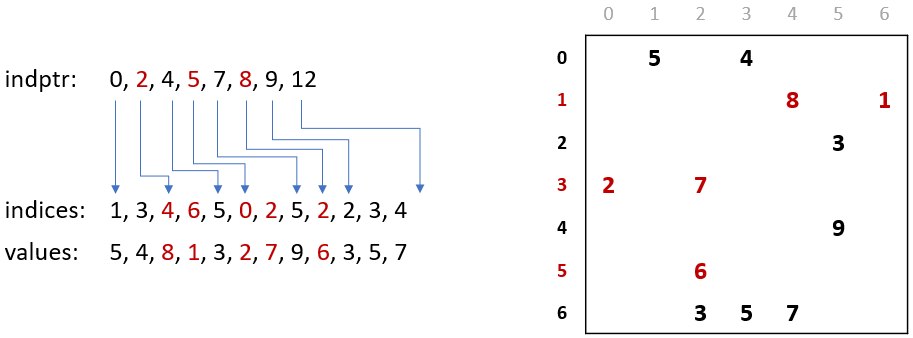
\includegraphics[width=4.5in]{GrB_CSR_FORMAT.png}
    \end{center}
    \caption{Data layout for CSR format.}
    \label{Fig:CSR_format}
    \hrule
\end{figure}

\subsection{{\sf GrB\_CSC\_FORMAT}}

The {\sf GrB\_CSC\_FORMAT} format indicates that a matrix will be imported or 
exported using the compressed sparse column (CSC) format.  {\sf indptr} is a 
pointer to an array of {\sf GrB\_Index} of size ncols+1 elements, where
the i'th index will contain the starting index in the {\sf values}
and {\sf indices} arrays corresponding to the i'th column of the matrix.
{\sf indices} is a pointer to an array of number of
stored elements (each a {\sf GrB\_Index}), where each element contains the 
corresponding element's row index within a column of the matrix.
{\sf values} is a pointer to an array of number of
stored elements (each the size of the scalar stored in the matrix) containing 
the corresponding value.  The 
elements of each column are not required to be sorted by row index.

\begin{figure}[h]
    \hrule
    \begin{center}
        ~\\
        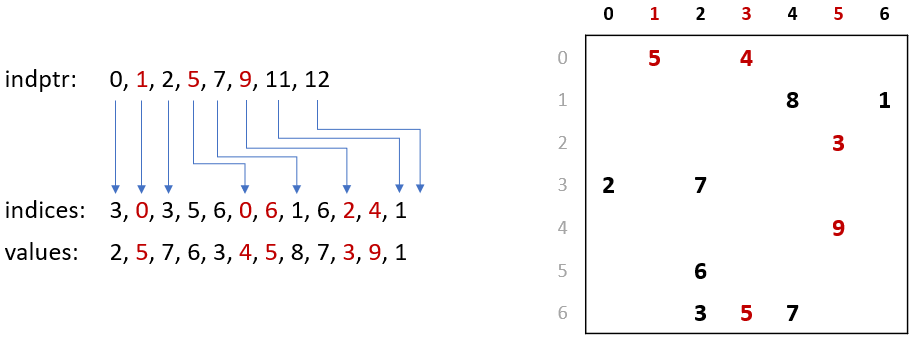
\includegraphics[width=4.5in]{GrB_CSC_FORMAT.png}
    \end{center}
    \vspace{-1em}
    \caption{Data layout for CSC format.}
    \label{Fig:CSC_format}
    \hrule
\end{figure}

\subsection{{\sf GrB\_COO\_FORMAT}}

The {\sf GrB\_COO\_FORMAT} format
indicates that a matrix will be imported or exported using the coordinate list
(COO) format.  {\sf indptr} is a pointer to an array of {\sf GrB\_Index} of size 
number of stored elements,
where each element contains the corresponding element's column index.
{\sf indices} will be a pointer to an array of {\sf GrB\_Index} of size 
number of stored elements, where each
element contains the corresponding element's row index.
{\sf values} will be a pointer to an array of size number of
stored elements (each the size of the scalar stored in the matrix) containing the corresponding value. Elements
are not required to be sorted in any order.

\begin{figure}[h]
    \hrule
    \begin{center}
        ~\\
        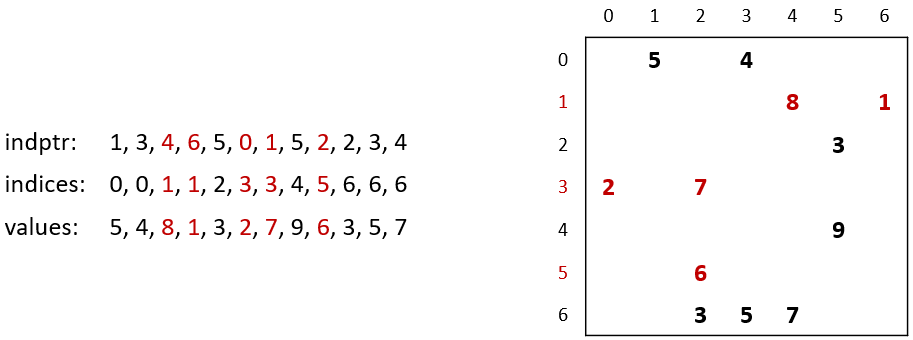
\includegraphics[width=4.5in]{GrB_COO_FORMAT.png}
    \end{center}
    \vspace{-1em}
    \caption{Data layout for COO format.}
    \label{Fig:COO_format}
    \hrule
\end{figure}

\comment{
\subsection{{\sf GrB\_DENSE\_ROW\_FORMAT}}

The {\sf GrB\_DENSE\_ROW\_FORMAT} format indicates that a matrix will be imported
or exported using the dense row-major format.  {\sf indptr} and {\sf indices} are unused,
and may be set to NULL, while {\sf values} will point to an array of size number of columns
times number of rows, where element i,j is located at index i*ncols + j. Elements will be
in the order they appear within each row, and rows will be in order.

\begin{figure}[h]
    \hrule
    \begin{center}
        ~\\
        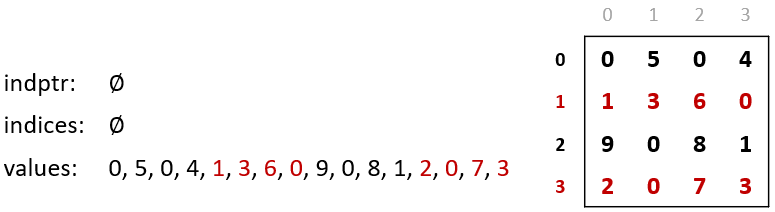
\includegraphics[width=4in]{GrB_DENSE_ROW_FORMAT.png}
    \end{center}
    \vspace{-1em}
    \caption{Data layout for the dense row-major format.}
    \label{Fig:DenseRow_format}
    \hrule
\end{figure}


\subsection{{\sf GrB\_DENSE\_COL\_FORMAT}}
The {\sf GrB\_DENSE\_COL\_FORMAT} format indicates that a matrix will be imported
or exported using the dense column-major format.  {\sf indptr} and {\sf indices} are unused,
and may be set to NULL, while {\sf values} will point to an array of size number of columns
times number of rows, where element i,j is located at index i + j*nrows. Elements will be
in the order they appear within each column, and columns will be in order.

\begin{figure}[h]
    \hrule
    \begin{center}
        ~\\
        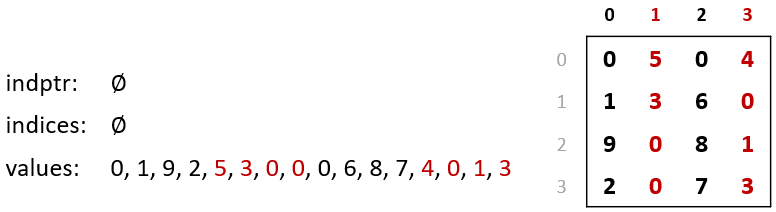
\includegraphics[width=4in]{GrB_DENSE_COLUMN_FORMAT.png}
    \end{center}
    \vspace{-1em}
    \caption{Data layout for the dense column-major format.}
    \label{Fig:DenseCol_format}
    \hrule
\end{figure}
}

%--------------------------------------------------------------
%--------------------------------------------------------------

\chapter{Examples}
\label{Chp:Examples}

\pagebreak
\nolinenumbers
\section{Example: Level breadth-first search (BFS) in GraphBLAS}
{\scriptsize
\lstinputlisting[language=C,numbers=left]{BFS5M.c}
}
\vfill

\pagebreak
\nolinenumbers
\section{Example: Level BFS in GraphBLAS using apply}
{\scriptsize
\lstinputlisting[language=C,numbers=left]{BFS6_apply.c}
}
\vfill

\pagebreak
\nolinenumbers
\section{Example: Parent BFS in GraphBLAS}
{\scriptsize
\lstinputlisting[language=C,numbers=left]{BFS7_parents.c}
}
\vfill

\pagebreak
\nolinenumbers
\section{Example: Betweenness centrality (BC) in GraphBLAS}
\label{App:BCnobatch}
{\scriptsize
\lstinputlisting[language=C,numbers=left]{BC1M_update.c}
}
\vfill

\pagebreak
\nolinenumbers
\section{Example: Batched BC in GraphBLAS}
{\scriptsize
\lstinputlisting[language=C,escapechar=|,numbers=left]{BC1_batch.c}
}
\vfill

\pagebreak
\nolinenumbers
\section{Example: Maximal independent set (MIS) in GraphBLAS}
{\scriptsize
\lstinputlisting[language=C,numbers=left]{MIS1.c}
}
\vfill

\pagebreak
\nolinenumbers
\section{Example: Counting triangles in GraphBLAS}
{\scriptsize
\lstinputlisting[language=C,numbers=left]{TC1.c}
}
\vfill
\pagebreak

\linenumbers


\end{document}
